\documentclass[letterpaper,10pt]{book}
% Change to 10 pt
\usepackage{pdfpages}
\usepackage{morewrites}			% to counteract the no write space problem
\setcounter{tocdepth}{6}

\usepackage[framemethod=TikZ]{mdframed}

\usepackage{fancyhdr}

\usepackage{paralist}
\usepackage{amsmath}
\usepackage{amsfonts}
\usepackage{amssymb}
\usepackage{graphicx}

\usepackage{datetime}
%\usepackage{ulem}

%\usepackage[nottoc]{toobibind}

\usepackage[inline]{enumitem}

% Outer margin at 2.50 is exacty correct to fit the ``corruption alert'' tables
\usepackage[inner=1.0in, outer=2.50in, top=2.54cm,bottom=2.54cm, marginparwidth=2.25in]{geometry}

\usepackage{marginnote}
\usepackage{longtable}
\usepackage{booktabs}
\usepackage{xcolor}

\usepackage{soul}

%%%%%%%%%%%%
\definecolor{ForestGreen}{rgb}{0.00,0.29,0.098}
%%%%%%%%%%%%

\usepackage{marginnote}

\usepackage{imakeidx} 
\usepackage[
	backref=true,
	style=numeric,
%	citestyle=numeric,
	backend=bibtex
	]{biblatex}
\usepackage[driverfallback=hypertex,colorlinks=True]{hyperref}
\usepackage{cleveref}

\makeindex[name=scripture,columnsep=20pt, columnseprule=True,columns=3, title=Scripture References]
\makeindex[name=speaker,columnsep=20pt, columnseprule=True,,columns=2, title=Sermon Creator]
\makeindex[name=series,columnsep=20pt, columnseprule=True,,columns=2, title=Sermon Series]
\makeindex[name=date,columnsep=20pt, columnseprule=True,columns=2, title=Sermon Date]
\makeindex[name=event,columnsep=20pt, columnseprule=True,columns=2, title=Event]
\makeindex[name=topic,columnsep=20pt, columnseprule=True,columns=2, title=Topic]
\makeindex[name=AWIP,columnsep=20pt, columnseprule=True,columns=3, title=All Words in Passage]
\makeindex[name=NWIV,columnsep=20pt, columnseprule=True,columns=3, title=Number of Words in Verse]
\makeindex[name=PNIP,columnsep=20pt, columnseprule=True,columns=3, title=Proper Names in Passage]
\makeindex[name=PEIP,columnsep=20pt, columnseprule=True,columns=2, title=Prophetic Events in Passage]
\makeindex[name=TWPAQ,columnsep=20pt, columnseprule=True,columns=1, title=13-Word Phrases and Quotes]
\makeindex[name=PFTTIS,columnsep=20pt, columnseprule=False,columns=3, title=Phrases found 13 times in scripture]
\makeindex[name=WFTTIS,columnsep=20pt, columnseprule=False,columns=3, title=Words found 13 times in scripture]
\makeindex[name=WFITV,columnsep=20pt, columnseprule=False,columns=3, title=Words found in exactly 13 verses]
\makeindex[name=EVENTS,columnsep=20pt, columnseprule=False,columns=2, title=Sermon Log by Place]
\makeindex[name=QUESTIONS,columnsep=20pt, columnseprule=False,columns=2, title=Bible Questions]
\makeindex[name=DOCTRINES,columnsep=20pt, columnseprule=False,columns=2, title=Doctrines]
\makeindex[name=SONGS,columnsep=20pt, columnseprule=False,columns=1, title=Songs]
\makeindex[name=LOCATION,columnsep=20pt, columnseprule=False,columns= 2, title=Location]
\makeindex[name=FACEBOOK,columnsep=20pt, columnseprule=False,columns=2, title=Facebook]
\makeindex[name=DEVOTIONAL,columnsep=20pt, columnseprule=False,columns=2, title=Devotional Items]
%%%%%%%%%%%%%%%%% EXTRA COLORS
\definecolor{champagne}{rgb}{0.97,0.91,0.81}
\definecolor{bone}{rgb}{0.89,0.85,0.79}
\pagestyle{fancy}
\fancyhf{}
\fancyhead[LE,RO]{\today}
\fancyhead[RE,LO]{Daily Bible Reading}
\fancyhead[CE,CO]{-page \thepage  - }

\fancyfoot[CO,CE]{\leftmark}
%\fancyfoot[LE,RO]{CSCE 692, HW1}

\title{DBR\\
Daily \\ Reads}
\author{Keith Anthony \\
\today }
%+/ffffff +   \pagenumbering{gobble}
\bibliography{Bibliographies/All20220122}

\setlength{\fboxsep}{1.0pt}

\usepackage[utf8]{inputenc}
\usepackage{tikz}

\begin{document}
%%%%%%%%%%%% Tile Page

\begin{titlepage}

\begin{flushright}
\rightskip=-2.5cm
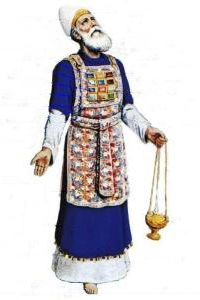
\includegraphics[width=50mm,scale=1.5]{Extras/Melchisedec.jpg}
\vspace{0.4in}  % Create a title for the document and write it in bold font
\LARGE{\textbf{\date}} % Again, do a line break
\linebreak 
% Create a subtitle \large{with Outlines, Statistics, Cross References, and Notes}
\vspace{0.5in}
\begin{flushleft}
\LARGE{Day \#68: Wednesday, 9 March 2022  \\}\vspace{0.25in}
\LARGE{Joshua 10-12 Psalm 68 Proverb 9}
\end{flushleft}
\vspace{0.6in}
\bigskip

\normalsize{Xenia, Oh.\\}
\normalsize{created: \today}
\vspace{1.3in}

\end{flushright}
\end{titlepage}

\newpage 
\tableofcontents\hypertarget{TOC}{}
\listoffigures
\listoftables

\hyphenation{A-bim-e-lech bre-thren E-phra-im  Gib-e-o-nites Jer-u-sa-lem through-out Phil-i-stines The-o-phil-us Am-a-le-kites ven-geance Mesh-el-e-mi-ah onan-ism Phar-a-oh thoughts grev-ous-ness Hach-a-liah adul-ter-er Shad-rach}

%%%%%%%%%%%%%%%%% EXTRA COLORS
%%%%%%%%%%%%%%%%% EXTRA COLORS
%%%%%%%%%%%%%%%%% EXTRA COLORS
\definecolor{champagne}{rgb}{0.97,0.91,0.81}
\definecolor{bone}{rgb}{0.89,0.85,0.79}

\definecolor{ForestGreen}{rgb}{0.00,0.29,0.098}
\definecolor{GIVING}{cmyk}{1,0.0,0.72,.1}

\definecolor{MLPE}{cmyk}{1,1,0,.45}
\definecolor{SOCCER}{cmyk}{.77, 0, .42, .49}
\definecolor{PAYBILL}{cmyk}{0,0.83,0.76,0.07}
\definecolor{SERMON}{cmyk}{.14,.9,0,.30} % aka seance \href{http://www.flatuicolorpicker.com/purple-cmyk-color-model/}{seance}
\definecolor{BIBLE}{cmyk}{0,.17,.74,.17}
\definecolor{WORKBLUE}{cmyk}{1, .5, 0, .6}
\definecolor{myOrange}{cmyk}{0, .4, .98, .03}
\definecolor{myTan}{cmyk}{0.0,.07,.17,.10}
\definecolor{myRed}{cmyk}{0,1,1,0}
\definecolor{myWhite}{cmyk}{0,0,0,0}
\definecolor{BLUESoD}{cmyk}{.97,.84,0,.04}
\definecolor{WHITE}{cmyk}{0,0,0,0}
\definecolor{OLDGOLD}{cmyk}{0.05,0.3,1.00,0}
\definecolor{CASTLETON}{cmyk}{1,0,0.31,0.66}
\definecolor{cadmiumgreen}{rgb}{0.0, 0.42, 0.24}
\definecolor{jungle}{rgb}{0.203,0.4882,0.1718}
\definecolor{MYGOLD}{rgb}{1,.84,0}

\definecolor{MYLIGHTGRAY}{rgb}{.85,.85,.85}

\definecolor{codegreen}{rgb}{0,0.6,0}
\definecolor{codegray}{rgb}{0.5,0.5,0.5}
\definecolor{codepurple}{rgb}{0.58,0,0.82}
\definecolor{backcolour}{rgb}{0.95,0.95,0.92}


\mdfdefinestyle{MyFrame}{%
    linecolor=blue,
    outerlinewidth=2pt,
    roundcorner=5pt,
    innertopmargin=\baselineskip,
    innerbottommargin=\baselineskip,
    innerrightmargin=10pt,
    innerleftmargin=10pt,
    backgroundcolor=gray!25!white}


\mdfdefinestyle{MyFrame2}{%
    linecolor=black,
    outerlinewidth=2pt,
    roundcorner=5pt,
    innertopmargin=\baselineskip,
    innerbottommargin=\baselineskip,
    innerrightmargin=10pt,
    innerleftmargin=10pt,
    backgroundcolor=yellow!25!white}


%%%%%
%% for PFTTIS list
%%%%%

%%% And Joseph said unto
\index[PFTTIS]{And Joseph said unto!Genesis!Gen 40:008}
\index[PFTTIS]{And Joseph said unto!Genesis!Gen 40:012}
\index[PFTTIS]{And Joseph said unto!Genesis!Gen 41:025}
\index[PFTTIS]{And Joseph said unto!Genesis!Gen 42:014}
\index[PFTTIS]{And Joseph said unto!Genesis!Gen 42:018}
\index[PFTTIS]{And Joseph said unto!Genesis!Gen 44:015}
\index[PFTTIS]{And Joseph said unto!Genesis!Gen 45:003}
\index[PFTTIS]{And Joseph said unto!Genesis!Gen 45:004}
\index[PFTTIS]{And Joseph said unto!Genesis!Gen 46:031}
\index[PFTTIS]{And Joseph said unto!Genesis!Gen 48:009}
\index[PFTTIS]{And Joseph said unto!Genesis!Gen 48:018}
\index[PFTTIS]{And Joseph said unto!Genesis!Gen 50:019}
\index[PFTTIS]{And Joseph said unto!Genesis!Gen 50:024}


%%% a shadow
\index[PFTTIS]{a shadow!1Chronicles!1Chr 029:15}
\index[PFTTIS]{a shadow!Job!Job 008:09}
\index[PFTTIS]{a shadow!Job!Job 014:02}
\index[PFTTIS]{a shadow!Job!Job 017:07}
\index[PFTTIS]{a shadow!Psalm!Psa 102:011}
\index[PFTTIS]{a shadow!Psalm!Psa 144:004}
\index[PFTTIS]{a shadow!Ecclesiastes!Eccl 006:012}
\index[PFTTIS]{a shadow!Ecclesiastes!Eccl 008:013}
\index[PFTTIS]{a shadow!Isaiah!Isa 04:006}
\index[PFTTIS]{a shadow!Isaiah!Isa 25:004}
\index[PFTTIS]{a shadow!Jonah!Jnh 04:06}
\index[PFTTIS]{a shadow!Colossians!Col 02:017}
\index[PFTTIS]{a shadow!Hebews!Heb 10:001}

%%% blessed is the man
\index[PFTTIS]{blessed is the man!Psalm!Psa 001:001}
\index[PFTTIS]{blessed is the man!Psalm!Psa 032:002}
\index[PFTTIS]{blessed is the man!Psalm!Psa 034:008}
\index[PFTTIS]{blessed is the man!Psalm!Psa 065:004}
\index[PFTTIS]{blessed is the man!Psalm!Psa 084:005}
\index[PFTTIS]{blessed is the man!Psalm!Psa 084:012}
\index[PFTTIS]{blessed is the man!Psalm!Psa 094:012}
\index[PFTTIS]{blessed is the man!Psalm!Psa 112:001}
\index[PFTTIS]{blessed is the man!Proverbs!Pro 008:034}
\index[PFTTIS]{blessed is the man!Isaiah!Isa 056:002}
\index[PFTTIS]{blessed is the man!Jeremiah!Jer 017:007}
\index[PFTTIS]{blessed is the man!Romans!Rom 004:008}
\index[PFTTIS]{blessed is the man!James!Jam 001:012}


%%% carry them
\index[PFTTIS]{carry them!Leviticus!Lev 14:045}
\index[PFTTIS]{carry them!Numbers!Num 11:012}
\index[PFTTIS]{carry them!Joshua!Jsh 04:003}
\index[PFTTIS]{carry them!1Samuel!1Sam 20:040}
\index[PFTTIS]{carry them!1Kings!1Kng 08:046}
\index[PFTTIS]{carry them!2Chronicles!2Chr 06:036}
\index[PFTTIS]{carry them!Ezra!Ezra 05:015}
\index[PFTTIS]{carry them!Isaiah!Isa 40:011}
\index[PFTTIS]{carry them!Isaiah!Isa 41:016}
\index[PFTTIS]{carry them!Isaiah!Isa 57:013}
\index[PFTTIS]{carry them!Jeremiah!Jer 20:004}
\index[PFTTIS]{carry them!Jeremiah!Jer 20:005}
\index[PFTTIS]{carry them!Jeremiah!Jer 43:012}


\index[PFTTIS]{good tidings!2Samuel!2Sam 18:027}
\index[PFTTIS]{good tidings!1Kings!1Ki 01:042}
\index[PFTTIS]{good tidings!2Kings!2Ki 07:009 (2x)}
\index[PFTTIS]{good tidings!Isaiah!Isa 40:009 (2x)}
\index[PFTTIS]{good tidings!Isaiah!Isa 41:007}
\index[PFTTIS]{good tidings!Isaiah!Isa 52:007}
\index[PFTTIS]{good tidings!Isaiah!Isa 61:001}
\index[PFTTIS]{good tidings!Nahum!Nah 01:005}
\index[PFTTIS]{good tidings!Luke!Lk 02:010}
\index[PFTTIS]{good tidings!1Thessalonians!1Thess 03:006}


%%% dead body
\index[PFTTIS]{dead body!Leviticus!Lev 21:011}
\index[PFTTIS]{dead body!Numbers!Num 06:006}
\index[PFTTIS]{dead body!Numbers!Num 09:006}
\index[PFTTIS]{dead body!Numbers!Num 09:007}
\index[PFTTIS]{dead body!Numbers!Num 09:010}
\index[PFTTIS]{dead body!Numbers!Num 09:011}
\index[PFTTIS]{dead body!Numbers!Num 09:013}
\index[PFTTIS]{dead body!Numbers!Num 09:016}
\index[PFTTIS]{dead body!2Kings!2Ki 08:005}
\index[PFTTIS]{dead body!Isaiah!Isa 26:019}
\index[PFTTIS]{dead body!Jeremiah!Jer 26:023}
\index[PFTTIS]{dead body!Jeremiah!Jer 36:030}
\index[PFTTIS]{dead body!Haggai!Hag 02:013}

%%% great sea
\index[PFTTIS]{great sea!Numbers!Num 34:006}
\index[PFTTIS]{great sea!Numbers!Num 34:007}
\index[PFTTIS]{great sea!Joshua!Jos 01:004}
\index[PFTTIS]{great sea!Joshua!Jos 09:001}
\index[PFTTIS]{great sea!Joshua!Jos 15:012}
\index[PFTTIS]{great sea!Joshua!Jos 15:047}
\index[PFTTIS]{great sea!Joshua!Jos 23:004}
\index[PFTTIS]{great sea!Ezekiel!Eze 47:010}
\index[PFTTIS]{great sea!Ezekiel!Eze 47:015}
\index[PFTTIS]{great sea!Ezekiel!Eze 47:019}
\index[PFTTIS]{great sea!Ezekiel!Eze 47:020}
\index[PFTTIS]{great sea!Ezekiel!Eze 48:028}
\index[PFTTIS]{great sea!Daniel!Dan 07:002}


%%% have forsaken me
\index[PFTTIS]{have forsaken me!Judges!Jdg 10:013}
\index[PFTTIS]{have forsaken me!1Samuel!1Sam 08:008}
\index[PFTTIS]{have forsaken me!1Kings!1Ki 11:033}
\index[PFTTIS]{have forsaken me!2Kings!2Ki 22:017}
\index[PFTTIS]{have forsaken me!2Chronicles!2Chr 12:005}
\index[PFTTIS]{have forsaken me!2Chronicles!2Chr 34:025}
\index[PFTTIS]{have forsaken me!Jeremiah!Jer 01:016}
\index[PFTTIS]{have forsaken me!Jeremiah!Jer 02:013}
\index[PFTTIS]{have forsaken me!Jeremiah!Jer 05:007}
\index[PFTTIS]{have forsaken me!Jeremiah!Jer 05:019}
\index[PFTTIS]{have forsaken me!Jeremiah!Jer 16:011 (2x)}
\index[PFTTIS]{have forsaken me!Jeremiah!Jer 19:004}

%%% no king
\index[PFTTIS]{no king!Judges!Jdg 17:06}
\index[PFTTIS]{no king!Judges!Jdg 18:01}
\index[PFTTIS]{no king!Judges!Jdg 19:01}
\index[PFTTIS]{no king!Judges!Jdg 21:25}
\index[PFTTIS]{no king!1Kings!1Ki 22:47}
\index[PFTTIS]{no king!2Kings!2Ki 23:25}
\index[PFTTIS]{no king!Nehemiah!Neh 13:26}
\index[PFTTIS]{no king!Psalms!Psa 033:016}
\index[PFTTIS]{no king!Proverbs!Pro 30:27}
\index[PFTTIS]{no king!Daniel!Dan 02:10}
\index[PFTTIS]{no king!Hosea!Hos 10:03}
\index[PFTTIS]{no king!Micah!Mic 04:09}
\index[PFTTIS]{no king!John!Jhn 19:15}


%%% rebellious house
\index[PFTTIS]{rebellious house!Exodus!Exo 02:005}
\index[PFTTIS]{rebellious house!Exodus!Exo 02:006}
\index[PFTTIS]{rebellious house!Exodus!Exo 02:008}
\index[PFTTIS]{rebellious house!Exodus!Exo 03:009}
\index[PFTTIS]{rebellious house!Exodus!Exo 03:026}
\index[PFTTIS]{rebellious house!Exodus!Exo 03:027}
\index[PFTTIS]{rebellious house!Exodus!Exo 12:002 (2x)}
\index[PFTTIS]{rebellious house!Exodus!Exo 12:003}
\index[PFTTIS]{rebellious house!Exodus!Exo 12:009}
\index[PFTTIS]{rebellious house!Exodus!Exo 12:025}
\index[PFTTIS]{rebellious house!Exodus!Exo 17:012}
\index[PFTTIS]{rebellious house!Exodus!Exo 24:003}

%%% seek him
\index[PFTTIS]{seek him!Deuteronomy!Deu 04:029}\index[PFTTIS]{seek him!1Samuel!1Sam 23:025}
\index[PFTTIS]{seek him!1Chronicles!1Chr 28:009}
\index[PFTTIS]{seek him!2Chronicles!1Chr 15:002}
\index[PFTTIS]{seek him!Ezra!Ezr 08:022}
\index[PFTTIS]{seek him!Psalms!Psa 022:026}
\index[PFTTIS]{seek him!Psalms!Psa 024:006}
\index[PFTTIS]{seek him!Psalms!Psa 119:002}
\index[PFTTIS]{seek him!SoS!SoS 03:002}
\index[PFTTIS]{seek him!SoS!SoS 06:001}
\index[PFTTIS]{seek him!Hosea!Hos 07:010}
\index[PFTTIS]{seek him!Amos!Amo 05:008}
\index[PFTTIS]{seek him!Hebrews!Heb 11:0063}


%%% seek ye
\index[PFTTIS]{seek ye!Isaiah!Isa 34:016}
\index[PFTTIS]{seek ye!Isaiah!Isa 45:019}
\index[PFTTIS]{seek ye!Isaiah!Isa 55:006}
\index[PFTTIS]{seek ye!Amos!Amos 5:004}
\index[PFTTIS]{seek ye!John!John 1:38}
\index[PFTTIS]{seek ye!John!John 18:4}
\index[PFTTIS]{seek ye!John!John 18:7}
\index[PFTTIS]{seek ye!Matthew!Matt 6:33}
\index[PFTTIS]{seek ye!Numbers!Num 16:10}
\index[PFTTIS]{seek ye!Luke!Luke 12:31}
\index[PFTTIS]{seek ye!Luke!Luke 24:5}
\index[PFTTIS]{seek ye!Psalm!Psa 27:8}
\index[PFTTIS]{seek ye!Zephaniah!Zeph 2:3}

%%% the uncircumcised
\index[PFTTIS]{the uncircumcised!Genesis!Gen 17:014}
\index[PFTTIS]{the uncircumcised!Judges!Jdg 14:003}
\index[PFTTIS]{the uncircumcised!Judges!Jdg 15:018}
\index[PFTTIS]{the uncircumcised!2Samuel!2Sam 01:020}
\index[PFTTIS]{the uncircumcised!Isaiah!Isa 02:001}
\index[PFTTIS]{the uncircumcised!Jeremiah!Jer 09:025}
\index[PFTTIS]{the uncircumcised!Ezekiel!Eze 28:010}
\index[PFTTIS]{the uncircumcised!Ezekiel!Eze 31:018}
\index[PFTTIS]{the uncircumcised!Ezekiel!Eze 32:019}
\index[PFTTIS]{the uncircumcised!Ezekiel!Eze 32:027}
\index[PFTTIS]{the uncircumcised!Ezekiel!Eze 32:028}
\index[PFTTIS]{the uncircumcised!Ezekiel!Eze 32:029}
\index[PFTTIS]{the uncircumcised!Ezekiel!Eze 32:032}

%%% worship him
\index[PFTTIS]{worship him!Psalms!Psa 97:007}
\index[PFTTIS]{worship him!Zephaniah!Zeph 02:011}
\index[PFTTIS]{worship him!Matthew!Matt 02:002}
\index[PFTTIS]{worship him!Matthew!Matt 02:008}
\index[PFTTIS]{worship him!John!John 04:023}
\index[PFTTIS]{worship him!John!John 04:024 (2x)} 
\index[PFTTIS]{worship him!Acts!Acts 17:023}
\index[PFTTIS]{worship him!Hebrews!Heb 01:006}
\index[PFTTIS]{worship him!Revelation!Rev 04:010}
\index[PFTTIS]{worship him!Revelation!Rev 13:008}
\index[PFTTIS]{worship him!Revelation!Rev 14:007}
\index[PFTTIS]{worship him!Revelation!Rev 19:010}


%%%%%
%% for PFTTIS list
%%%%%

%%% afflictions
\index[WFTTIS]{afflictions!Psalms!Psa 34:019}
\index[WFTTIS]{afflictions!Psalms!Psa 132:001}
\index[WFTTIS]{afflictions!Acts!Acts 07:010}
\index[WFTTIS]{afflictions!Acts!Acts 20:023}
\index[WFTTIS]{afflictions!2Corinthians!2Cor 06:004}
\index[WFTTIS]{afflictions!Colossians!Col 01:024}
\index[WFTTIS]{afflictions!1Thessalonians!1Thess 03:003}
\index[WFTTIS]{afflictions!2Timothy!2Tim 01:008}
\index[WFTTIS]{afflictions!2Timothy!2Tim 03:011}
\index[WFTTIS]{afflictions!2Timothy!2Tim 04:005}
\index[WFTTIS]{afflictions!Hebrews!Heb 10:032}
\index[WFTTIS]{afflictions!Hebrews!Heb 10:033}
\index[WFTTIS]{afflictions!1Peter!1Pet 05:009}

%%% acsend
\index[WFTTIS]{acsend!Joshua!Jos 06:05}
\index[WFTTIS]{acsend!Psalm!Psa 024:003}
\index[WFTTIS]{acsend!Psalm!Psa 135:007}
\index[WFTTIS]{acsend!Psalm!Psa 139:008}
\index[WFTTIS]{acsend!Isaiah!Isa 14:013}
\index[WFTTIS]{acsend!Isaiah!Isa 14:014}
\index[WFTTIS]{acsend!Jeremiah!Jer 10:013}
\index[WFTTIS]{acsend!Jeremiah!Jer 51:016}
\index[WFTTIS]{acsend!Ezekiel!Eze 38:009}
\index[WFTTIS]{acsend!John!John 06:062}
\index[WFTTIS]{acsend!John!John 20:017}
\index[WFTTIS]{acsend!Romans!Rom 10:006}
\index[WFTTIS]{acsend!Revelation!Rev 17:008}

%%% Assyrian
\index[WFTTIS]{Assyrian!Isaiah!Isa 10:005}
\index[WFTTIS]{Assyrian!Isaiah!Isa 10:024}
\index[WFTTIS]{Assyrian!Isaiah!Isa 14:025}
\index[WFTTIS]{Assyrian!Isaiah!Isa 19:023}
\index[WFTTIS]{Assyrian!Isaiah!Isa 23:013}
\index[WFTTIS]{Assyrian!Isaiah!Isa 30:031}
\index[WFTTIS]{Assyrian!Isaiah!Isa 31:008}
\index[WFTTIS]{Assyrian!Isaiah!Isa 52:004}
\index[WFTTIS]{Assyrian!Ezekiel!Eze 31:003}
\index[WFTTIS]{Assyrian!Hosea!Hos 05:013}
\index[WFTTIS]{Assyrian!Hosea!Hos 11:005}
\index[WFTTIS]{Assyrian!Micah!Hos 05:005}
\index[WFTTIS]{Assyrian!Micah!Hos 05:006}

%%% blot
\index[WFTTIS]{blot!Exodus!Exo 32:032}
\index[WFTTIS]{blot!Exodus!Exo 32:033}
\index[WFTTIS]{blot!Numbers!Num 05:026}
\index[WFTTIS]{blot!Deuteronomy!Deut 09:014}
\index[WFTTIS]{blot!Deuteronomy!Deut 25:019}
\index[WFTTIS]{blot!Deuteronomy!Deut 29:020}
\index[WFTTIS]{blot!2Kings!2Ki 14:027}
\index[WFTTIS]{blot!Job!Job 31:007}
\index[WFTTIS]{blot!Psalms!Psa 51:001}
\index[WFTTIS]{blot!Psalms!Psa 51:009}
\index[WFTTIS]{blot!Proverbs!Pro 09:007}
\index[WFTTIS]{blot!Jeremiah!Jer 18:023}
\index[WFTTIS]{blot!Revelation!Rev 03:005}


%%% chain
\index[WFTTIS]{chain!Genesis!Gen 41:042}
\index[WFTTIS]{chain!1Kings!1Ki 07:017}
\index[WFTTIS]{chain!Psalms!Psa 73:006}
\index[WFTTIS]{chain!SoS!Sos 04:009}
\index[WFTTIS]{chain!Lamentations!Lam 03:007}
\index[WFTTIS]{chain!Ezekiel!Eze 07:023}
\index[WFTTIS]{chain!Ezekiel!Eze 16:011}
\index[WFTTIS]{chain!Daniel!Dan 05:007}
\index[WFTTIS]{chain!Daniel!Dan 05:016}
\index[WFTTIS]{chain!Daniel!Dan 05:029}
\index[WFTTIS]{chain!Acts!Acts 28:020}
\index[WFTTIS]{chain!2Timothy!2Tim 01:016}
\index[WFTTIS]{chain!Revelation!Rev 20:001}


%%% controversy
\index[WFTTIS]{controversy!Deuteronomy!Deu 17:008}
\index[WFTTIS]{controversy!Deuteronomy!Deu 19:017}
\index[WFTTIS]{controversy!Deuteronomy!Deu 21:005}
\index[WFTTIS]{controversy!Deuteronomy!Deu 25:001}
\index[WFTTIS]{controversy!2Samuel!2Sam 15:002}
\index[WFTTIS]{controversy!Isaiah!Isa 34:008}
\index[WFTTIS]{controversy!Jeremiah!Jer 25:031}
\index[WFTTIS]{controversy!Ezekiel!Eze 44:024}
\index[WFTTIS]{controversy!Hosea!Hos 04:001}
\index[WFTTIS]{controversy!Hosea!Hos 12:002}
\index[WFTTIS]{controversy!Micah!Mic 06:002 (2x)}
\index[WFTTIS]{controversy!1Timothy!1Tim 03:016}


%%% Dagon/Dagon's
\index[WFTTIS]{Dagon!Judges!Jdg 16:023}
\index[WFTTIS]{Dagon!1Samuel!1Sam 05:002 (2x)}
\index[WFTTIS]{Dagon!1Samuel!1Sam 05:003 (2x)}
\index[WFTTIS]{Dagon!1Samuel!1Sam 05:004 (3x)}
\index[WFTTIS]{Dagon!1Samuel!1Sam 05:005 (3x)}
\index[WFTTIS]{Dagon!1Samuel!1Sam 05:007}
\index[WFTTIS]{Dagon!1Chronicles!1Chr 10:010}

%%% disobedient
\index[WFTTIS]{disobedient!1Kings!1Ki 13:026}
\index[WFTTIS]{disobedient!Nehemiah!Neh 09:026}
\index[WFTTIS]{disobedient!Luke!Luke 01:017}
\index[WFTTIS]{disobedient!Acts!Acts 26:019}
\index[WFTTIS]{disobedient!Romans!Rom 01:030}
\index[WFTTIS]{disobedient!Romans!Rom 10:021}
\index[WFTTIS]{disobedient!1Timothy!1Tim 01:009}
\index[WFTTIS]{disobedient!2Timothy!2Tim 03:002}
\index[WFTTIS]{disobedient!Titus!Titus 01:016}
\index[WFTTIS]{disobedient!Titus!Titus 03:003}
\index[WFTTIS]{disobedient!1Peter!1Pet 02:007}
\index[WFTTIS]{disobedient!1Peter!1Pet 02:008}
\index[WFTTIS]{disobedient!1Peter!1Pet 03:020}


%%% doubt
\index[WFTTIS]{doubt!Genesis!Gen 37:033}
\index[WFTTIS]{doubt!Deuteronomy!Deu 28:066}
\index[WFTTIS]{doubt!Job!Job 12:002}
\index[WFTTIS]{doubt!Matthew!Matt 14:031}
\index[WFTTIS]{doubt!Matthew!Matt 21:021}
\index[WFTTIS]{doubt!Mark!Mk 11:023}
\index[WFTTIS]{doubt!Luke!Lk 11:020}
\index[WFTTIS]{doubt!John!Jhn 10:024}
\index[WFTTIS]{doubt!Acts!Acts 02:012}
\index[WFTTIS]{doubt!Acts!Acts 28:004}
\index[WFTTIS]{doubt!1Corinthians!1Cor 09:010}
\index[WFTTIS]{doubt!Galatians!Gal 04:020}
\index[WFTTIS]{doubt!1John!1Jhn 02:019}


%%% dungeon
\index[WFTTIS]{dungeon!Genesis!Gen 40:015}
\index[WFTTIS]{dungeon!Genesis!Gen 41:014}
\index[WFTTIS]{dungeon!Exodus!Exo 12:029}
\index[WFTTIS]{dungeon!Jeremiah!Jer 37:016}
\index[WFTTIS]{dungeon!Jeremiah!Jer 38:006 (2x)}
\index[WFTTIS]{dungeon!Jeremiah!Jer 38:007}
\index[WFTTIS]{dungeon!Jeremiah!Jer 38:009}
\index[WFTTIS]{dungeon!Jeremiah!Jer 38:010}
\index[WFTTIS]{dungeon!Jeremiah!Jer 38:011}
\index[WFTTIS]{dungeon!Jeremiah!Jer 38:013}
\index[WFTTIS]{dungeon!Lamentations!Lam 03:053}
\index[WFTTIS]{dungeon!Lamentations!Lam 03:055}


%%% error
\index[WFTTIS]{error!2Samuel!2Sam 06:007}
\index[WFTTIS]{error!Job!Job 19:004}
\index[WFTTIS]{error!Ecclesiastes!Ecc 05:006}
\index[WFTTIS]{error!Ecclesiastes!Ecc 10:005}
\index[WFTTIS]{error!Isaiah!Isa 32:006}
\index[WFTTIS]{error!Daniel!Dan 06:004}
\index[WFTTIS]{error!Matthew!Matt 27:064}
\index[WFTTIS]{error!Romans!Rom 01:027}
\index[WFTTIS]{error!James!Jam 05:020}
\index[WFTTIS]{error!2Peter!2Pet 02:018}
\index[WFTTIS]{error!2Peter!2Pet 03:017}
\index[WFTTIS]{error!1John!1Jn 04:006}
\index[WFTTIS]{error!Jude!Jude 01:011}

%%% fourish
\index[WFTTIS]{fourish!Psalms!Psa 072:007}
\index[WFTTIS]{fourish!Psalms!Psa 072:016}
\index[WFTTIS]{fourish!Psalms!Psa 092:007}
\index[WFTTIS]{fourish!Psalms!Psa 092:012}
\index[WFTTIS]{fourish!Psalms!Psa 092:013}
\index[WFTTIS]{fourish!Psalms!Psa 132:018}
\index[WFTTIS]{fourish!Proverbs!Pro 11:28}
\index[WFTTIS]{fourish!Proverbs!Pro 14:11}
\index[WFTTIS]{fourish!Ecclesiastes!Ecc 12:05}
\index[WFTTIS]{fourish!SongOfSolomon!SOS 07:12}
\index[WFTTIS]{fourish!Isaiah!Isa 17:11}
\index[WFTTIS]{fourish!Isaiah!Isa 66:14}
\index[WFTTIS]{fourish!Ezekiel!Eze 17:24}




%%% giants
\index[WFTTIS]{giants!Genesis!Gen 06:004}
\index[WFTTIS]{giants!Numbers!Num 13:033}
\index[WFTTIS]{giants!Deuteronomy!Deut 02:011}
\index[WFTTIS]{giants!Deuteronomy!Deut 02:021}
\index[WFTTIS]{giants!Deuteronomy!Deut 03:011}
\index[WFTTIS]{giants!Deuteronomy!Deut 03:013}
\index[WFTTIS]{giants!Joshua!Josh 12:004}
\index[WFTTIS]{giants!Joshua!Josh 13:012}
\index[WFTTIS]{giants!Joshua!Josh 15:008}
\index[WFTTIS]{giants!Joshua!Josh 17:015}
\index[WFTTIS]{giants!Joshua!Josh 16:016}

%%% good man
\index[WFTTIS]{good man!2 Samuel!2Sa 18:27}
%(1) Psalms 37:23 [5]
%(1) Psalms 112:5 [2]
%(1) Proverbs 12:2 [2]
%(1) Proverbs 13:22 [2]
%(1) Proverbs 14:14 [14]
%(1) Micah 7:2 [2]
%(1) Matthew 12:35 [2]
%(1) Luke 6:45 [2]
%(1) Luke 23:50 [15]
%(1) John 7:12 [17]
%(1) Acts 11:24 [5]
%(1) Romans 5:7 [14]

%%% Hinnom
\index[WFTTIS]{Hinnom!Joshua!Jsh 15:008}
\index[WFTTIS]{Hinnom!Joshua!Jsh 18:016}
\index[WFTTIS]{Hinnom!2Kings!2Ki 23:010}
\index[WFTTIS]{Hinnom!2Chronicles!2Chr 28:003}
\index[WFTTIS]{Hinnom!2Chronicles!2Chr 33:006}
\index[WFTTIS]{Hinnom!Nehemiah!Neh 11:030}
\index[WFTTIS]{Hinnom!Jeremiah!Jer 07:031}
\index[WFTTIS]{Hinnom!Jeremiah!Jer 07:032}
\index[WFTTIS]{Hinnom!Jeremiah!Jer 19:002}
\index[WFTTIS]{Hinnom!Jeremiah!Jer 19:006}
\index[WFTTIS]{Hinnom!Jeremiah!Jer 32:035}

%%% inclined
\index[WFTTIS]{inclined!Judges!Jdg 09:003}
\index[WFTTIS]{inclined!Psalms!Psa 040:001}
\index[WFTTIS]{inclined!Psalms!Psa 116:002}
\index[WFTTIS]{inclined!Psalms!Psa 119:112}
\index[WFTTIS]{inclined!Proverbs!Pro 05:13}
\index[WFTTIS]{inclined!Jeremiah!Jer 07:24}
\index[WFTTIS]{inclined!Jeremiah!Jer 07:26}
\index[WFTTIS]{inclined!Jeremiah!Jer 11:08}
\index[WFTTIS]{inclined!Jeremiah!Jer 17:23}
\index[WFTTIS]{inclined!Jeremiah!Jer 25:04}
\index[WFTTIS]{inclined!Jeremiah!Jer 34:14}
\index[WFTTIS]{inclined!Jeremiah!Jer 35:15}
\index[WFTTIS]{inclined!Jeremiah!Jer 44:05}


%%% laughed
\index[WFTTIS]{laughed!Genesis!Gen 17:017}
\index[WFTTIS]{laughed!Genesis!Gen 18:012}
\index[WFTTIS]{laughed!Genesis!Gen 18:015}
\index[WFTTIS]{laughed!2Kings!2Ki 19:021}
\index[WFTTIS]{laughed!2Chronicles!2Chr 30:010}
\index[WFTTIS]{laughed!Nehemiah!Neh 02:019}
\index[WFTTIS]{laughed!Job!Job 12:004}
\index[WFTTIS]{laughed!Job!Job 29:024}
\index[WFTTIS]{laughed!Isaiah!Isa 37:022}
\index[WFTTIS]{laughed!Ezekiel!Ezek 23:032}
\index[WFTTIS]{laughed!Matthew!Matt 09:024}
\index[WFTTIS]{laughed!Mark!Mk 05:040}
\index[WFTTIS]{laughed!Luke!Lk 08:053}

%%% liar
\index[WFTTIS]{liar!Job!Job 24:025}
\index[WFTTIS]{liar!Proverbs!Pro 17:004}
\index[WFTTIS]{liar!Proverbs!Pro 19:022}
\index[WFTTIS]{liar!Proverbs!Pro 30:006}
\index[WFTTIS]{liar!Jeremiah!Jer 15:018}
\index[WFTTIS]{liar!John!Jhn 08:044}
\index[WFTTIS]{liar!John!Jhn 08:055}
\index[WFTTIS]{liar!Romans!Rom 03:004}
\index[WFTTIS]{liar!1John!1Jhn 01:010}
\index[WFTTIS]{liar!1John!1Jhn 02:004}
\index[WFTTIS]{liar!1John!1Jhn 02:022}
\index[WFTTIS]{liar!1John!1Jhn 04:020}
\index[WFTTIS]{liar!1John!1Jhn 05:010}

%%% palsy
\index[WFTTIS]{palsy!Matthew!Matt 04:024}
\index[WFTTIS]{palsy!Matthew!Matt 08:006}
\index[WFTTIS]{palsy!Matthew!Matt 09:002}
\index[WFTTIS]{palsy!Matthew!Matt 09:006}
\index[WFTTIS]{palsy!Mark!Mk 02:003}
\index[WFTTIS]{palsy!Mark!Mk 02:004}
\index[WFTTIS]{palsy!Mark!Mk 02:005}
\index[WFTTIS]{palsy!Mark!Mk 02:009}
\index[WFTTIS]{palsy!Mark!Mk 02:010}
\index[WFTTIS]{palsy!Luke!Lk 05:018}
\index[WFTTIS]{palsy!Luke!Lk 05:024}
\index[WFTTIS]{palsy!Acts!Acts 09:033}

%%% Profitable
\index[WFTTIS]{profitable!Job!Job 22:002 (2x)}
\index[WFTTIS]{profitable!Ecclesiastes!Ecc 10:010}
\index[WFTTIS]{profitable!Isaiah!Isa 44:010}
\index[WFTTIS]{profitable!Jeremiah!Jer 13:007}
\index[WFTTIS]{profitable!Matthew!Matt 05:029}
\index[WFTTIS]{profitable!Matthew!Matt 05:030}
\index[WFTTIS]{profitable!Acts!Acts 20:020}
\index[WFTTIS]{profitable!1Timothy!1Tim 04:008}
\index[WFTTIS]{profitable!2Timothy!2Tim 03:016}
\index[WFTTIS]{profitable!2Timothy!2Tim 04:011}
\index[WFTTIS]{profitable!Titus!Titus 03:008}
\index[WFTTIS]{profitable!Philemon!Phlm 01:011}

%%% Rechab
\index[WFTTIS]{Rechab!2Samuel!2Sam 04:002}
\index[WFTTIS]{Rechab!2Samuel!2Sam 04:005}
\index[WFTTIS]{Rechab!2Samuel!2Sam 04:006}
\index[WFTTIS]{Rechab!2Samuel!2Sam 04:009}
\index[WFTTIS]{Rechab!2KIngs!2Ki 10:015}
\index[WFTTIS]{Rechab!2KIngs!2Ki 10:023}
\index[WFTTIS]{Rechab!1Chronicles!1Chr 02:055}
\index[WFTTIS]{Rechab!Nehemiah!Neh 03:014}
\index[WFTTIS]{Rechab!Jeremiah!Jer 35:006}
\index[WFTTIS]{Rechab!Jeremiah!Jer 35:008}
\index[WFTTIS]{Rechab!Jeremiah!Jer 35:014}
\index[WFTTIS]{Rechab!Jeremiah!Jer 35:016}
\index[WFTTIS]{Rechab!Jeremiah!Jer 35:019}

%%% serpents
\index[WFTTIS]{serpents!Exodus!Exo 07:012}
\index[WFTTIS]{serpents!Numbers!Num 21:006}
\index[WFTTIS]{serpents!Numbers!Num 21:007}
\index[WFTTIS]{serpents!Deuteronomy!Deu 08:015}
\index[WFTTIS]{serpents!Deuteronomy!Deu 32:024}
\index[WFTTIS]{serpents!Jeremiah!Jer 08:017}
\index[WFTTIS]{serpents!Matthew!Matt 10:016}
\index[WFTTIS]{serpents!Matthew!Matt 23:033}
\index[WFTTIS]{serpents!Mark!Mk 16:018}
\index[WFTTIS]{serpents!Luke!Lk 10:019}
\index[WFTTIS]{serpents!1Corinthians!1Cor 10:009}
\index[WFTTIS]{serpents!James!Jas 03:007}
\index[WFTTIS]{serpents!Revelation!Rev 09:019}

%%% short
\index[WFTTIS]{short!Numbers!Num 11:023}
\index[WFTTIS]{short!2Kings!2Ki 10:032}
\index[WFTTIS]{short!Job!Job 17:012}
\index[WFTTIS]{short!Job!Job 20:005}
\index[WFTTIS]{short!Psalms!Psa 89:047}
\index[WFTTIS]{short!Romans!Rom 03:023}
\index[WFTTIS]{short!Romans!Rom 09:028  (2x)}
\index[WFTTIS]{short!1Corinthians!1Cor 07:029}
\index[WFTTIS]{short!1Thessalonians!1Thess 02:017}
\index[WFTTIS]{short!Hebrews!Heb 04:001}
\index[WFTTIS]{short!Revelation!Rev 12:012}
\index[WFTTIS]{short!Revelation!Rev 17:010}

%%% smiteth
\index[WFTTIS]{smiteth!Exodus!Exo 21:012}
\index[WFTTIS]{smiteth!Exodus!Exo 21:15}
\index[WFTTIS]{smiteth!Deuteronomy!Dt 25:11}
\index[WFTTIS]{smiteth!Deuteronomy!Dt 27:24}
\index[WFTTIS]{smiteth!Joshua!Jsh 15:16}
\index[WFTTIS]{smiteth!Judges!Jdg 15:16}
\index[WFTTIS]{smiteth!2 Samuel!2Sa 05:08}
\index[WFTTIS]{smiteth!1Chronicles!1Chr 11:06}
\index[WFTTIS]{smiteth!Job!1Chr 26:12}
\index[WFTTIS]{smiteth!Isaiah!Isa 09:13}
\index[WFTTIS]{smiteth!Lamentations!Lam 03:30}
\index[WFTTIS]{smiteth!Ezekiel!Eze 07:09}
\index[WFTTIS]{smiteth!Luke!Lk 06:29}



%%% vanities
\index[WFTTIS]{vanities!Deuteronomy!Deut 21:021}
\index[WFTTIS]{vanities!1Kings!1Ki 16:013}
\index[WFTTIS]{vanities!1Kings!1Ki 16:026}
\index[WFTTIS]{vanities!Psalms!Psa 031:006}
\index[WFTTIS]{vanities!Ecclesiastes!Ecc 01:002 (2x)}
\index[WFTTIS]{vanities!Ecclesiastes!Ecc 05:007}
\index[WFTTIS]{vanities!Ecclesiastes!Ecc 12:008}
\index[WFTTIS]{vanities!Jeremiah!Jer 08:019}
\index[WFTTIS]{vanities!Jeremiah!Jer 10:008}
\index[WFTTIS]{vanities!Jeremiah!Jer 14:022}
\index[WFTTIS]{vanities!Jonah!Jnh 02:008}
\index[WFTTIS]{vanities!Acts!Acts 14:015}



%%%%%
%% for PFTTIS list
%%%%%

%%% worm
\index[WFITV]{worm!Exodus!Exo 16:024}
\index[WFITV]{worm!Job!Job 17:014}
\index[WFITV]{worm!Job!Job 24:029}
\index[WFITV]{worm!Job!Job 25:005 (2x)}
\index[WFITV]{worm!Psalms!Psa 022:006}
\index[WFITV]{worm!Isaiah!Isa 14:011}
\index[WFITV]{worm!Isaiah!Isa 41:014}
\index[WFITV]{worm!Isaiah!Isa 51:008}
\index[WFITV]{worm!Isaiah!Isa 66:024}
\index[WFITV]{worm!Jonah!Jnh 04:007}
\index[WFITV]{worm!Mark!Mk 09:044}
\index[WFITV]{worm!Mark!Mk 09:046}
\index[WFITV]{worm!Mark!Mk 09:048}


%\subsubsection{Title}
%\textbf{Introduction:} Isaiah 46 
%\index[speaker]{Speaker!Isaiah 49 (Title}
%\index[series]{Book (Speaker)!IPassage (Title)}
%\index[date]{2017/07/09!Isaiah 49 (Title)}
%\begin{compactenum}[I.]
%    \item  \textbf{Point} \index[scripture]{Isaiah!IPassage} (IPassage)
%\end{compactenum}




  


%\input{02OT-Exodus/ExodusIntroduction}

%\newpage
%\begin{figure}
%\begin{center}
%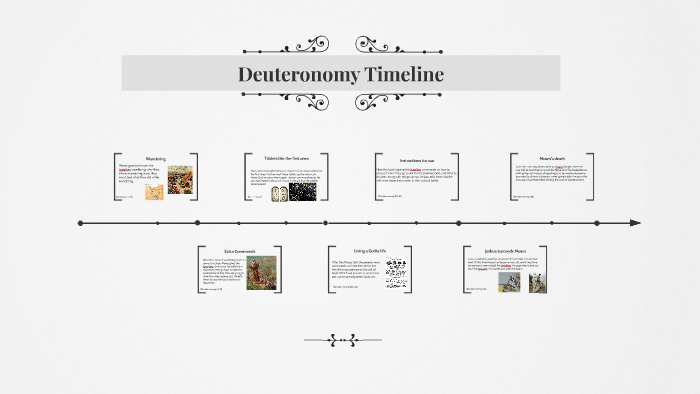
\includegraphics[scale=.7, angle=0]{05OT-Deuteronomy/References/AndrewSmithDeuteronomyTimeline.png}
%\caption[Deuteronomy Timeline by Andrew Smith]{Deuteronomy Timeline by Andrew %Smith}
%\label{fig:Deuteronomy Timeline by Andrew Smith}
%\end{center}
%\end{figure}

\newpage
\begin{figure}
\begin{center}
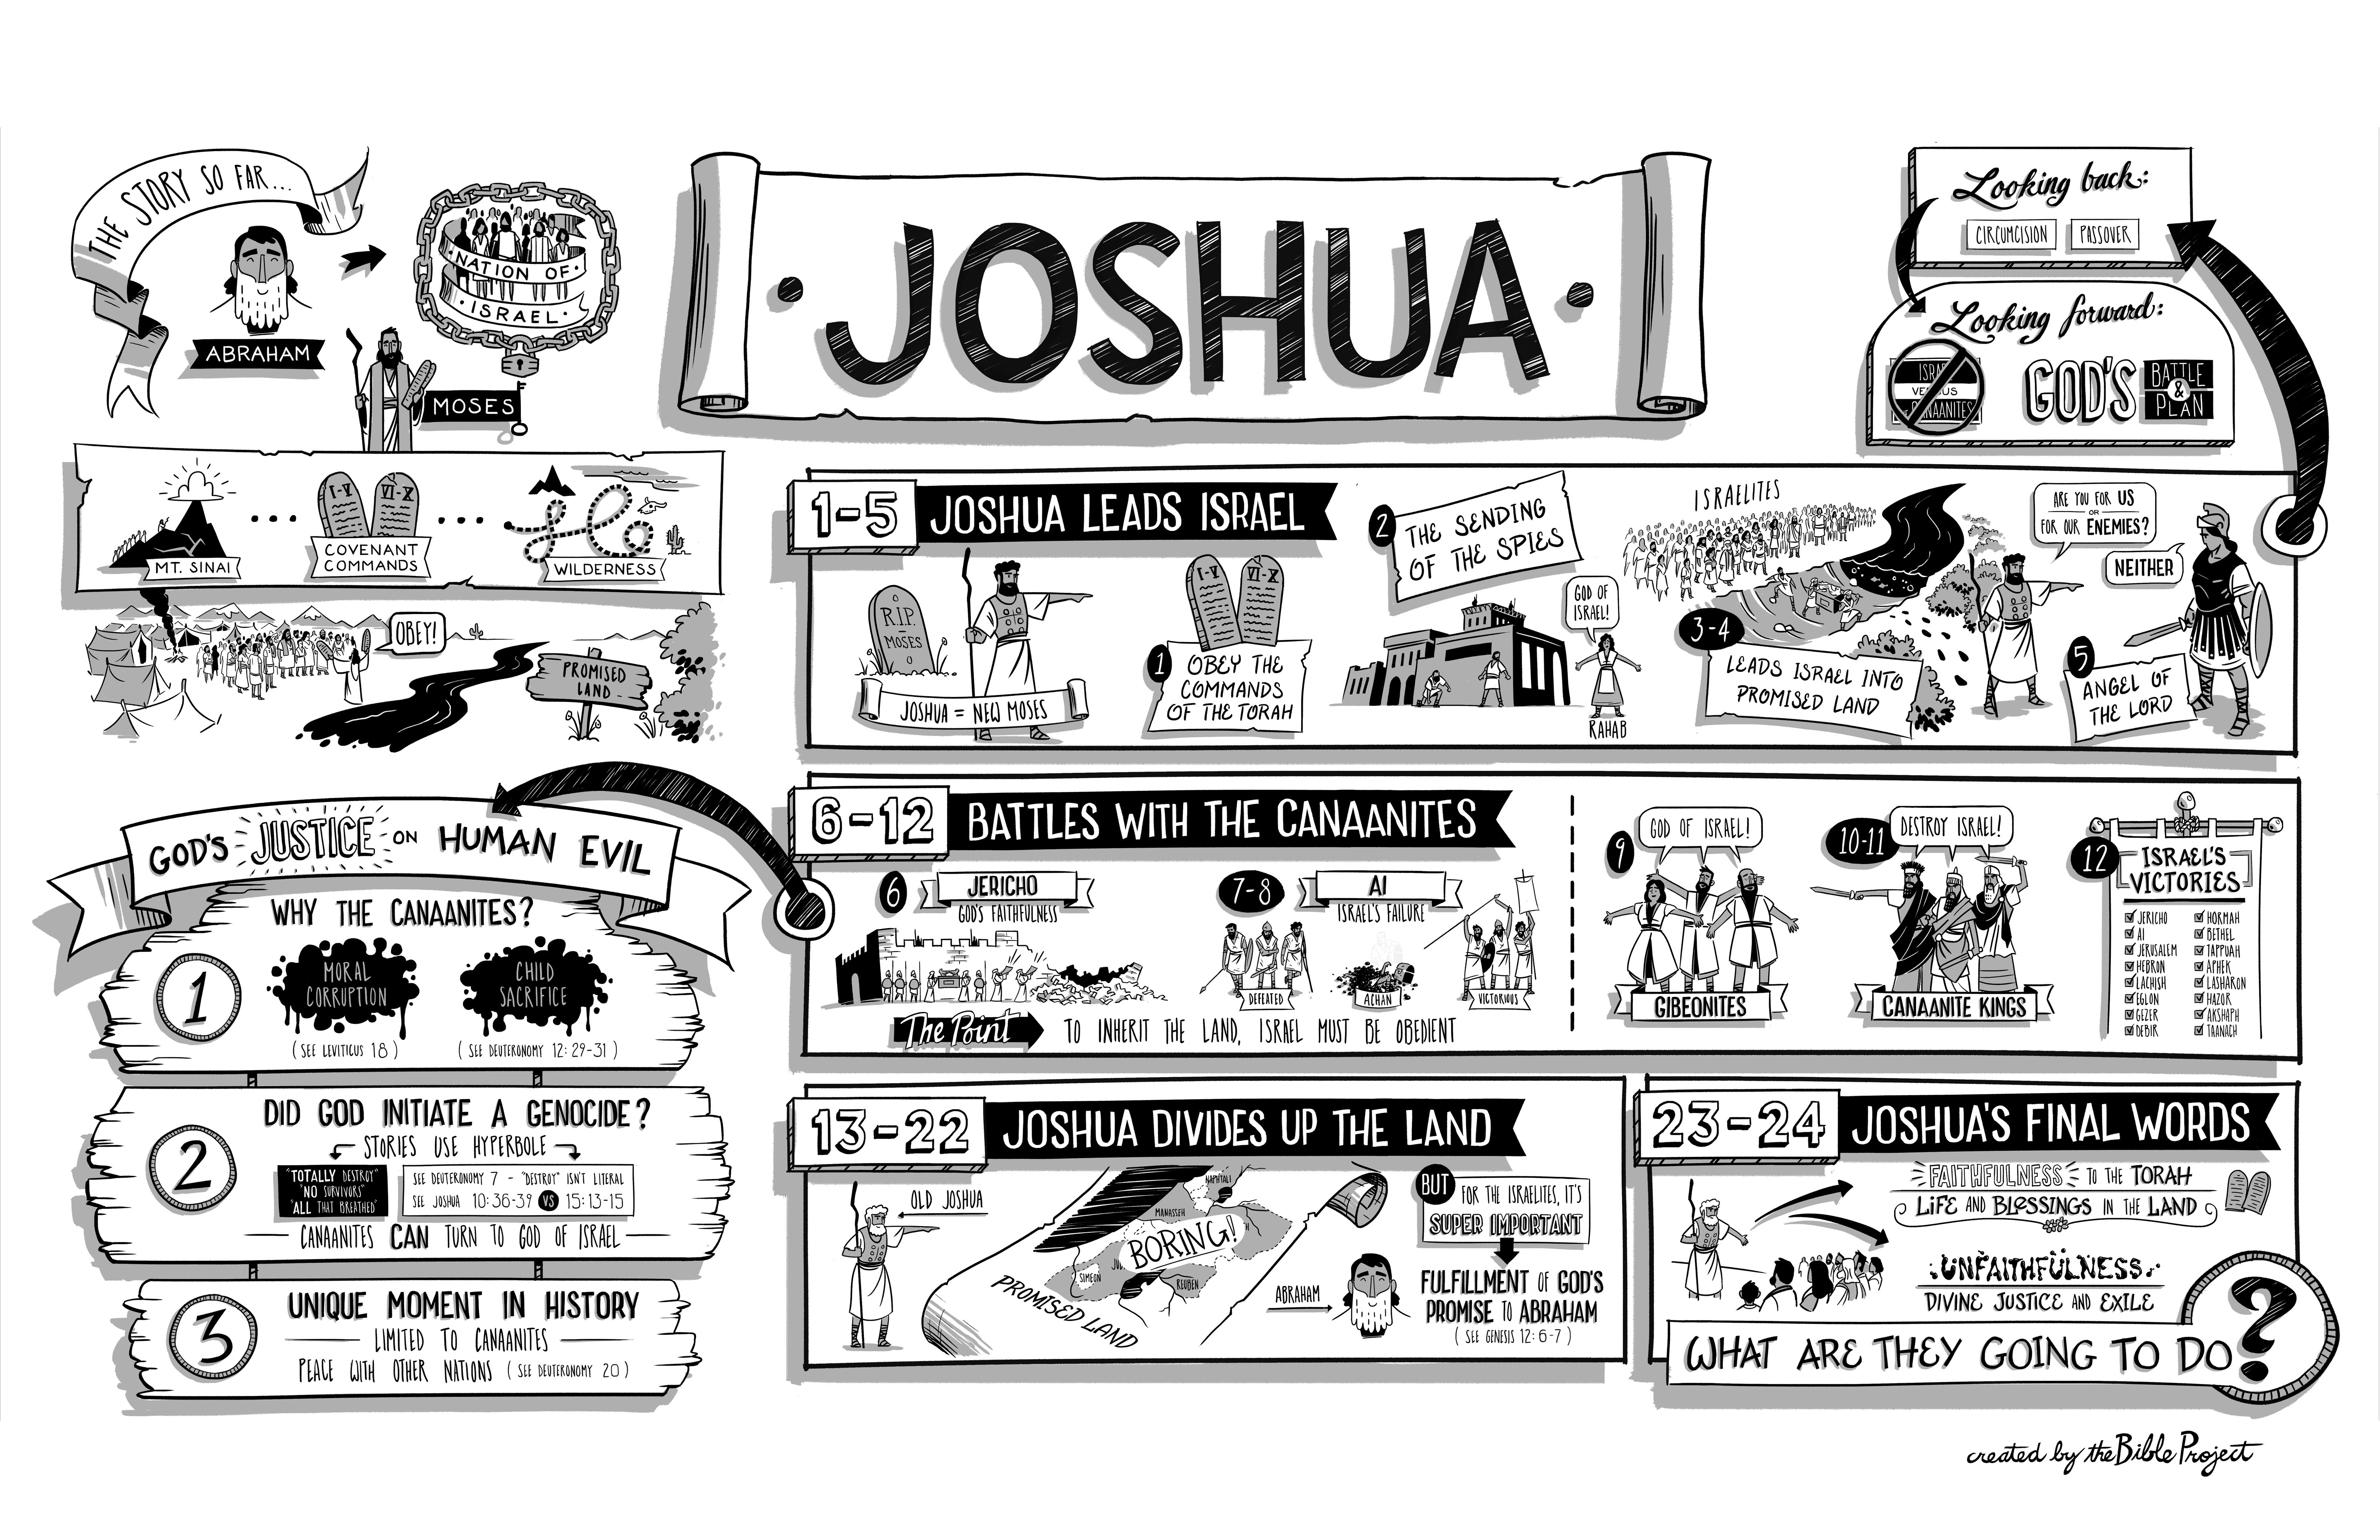
\includegraphics[scale=0.5, angle=90]{06OT-Joshua/References/1.BibleProject-Joshua.jpg}
\caption[Joshua from the Bible Project]{Joshua from the Bible Project}
\label{fig:Joshua from the Bible Project}
\end{center}
\end{figure}

\newpage
\begin{figure}
\begin{center}
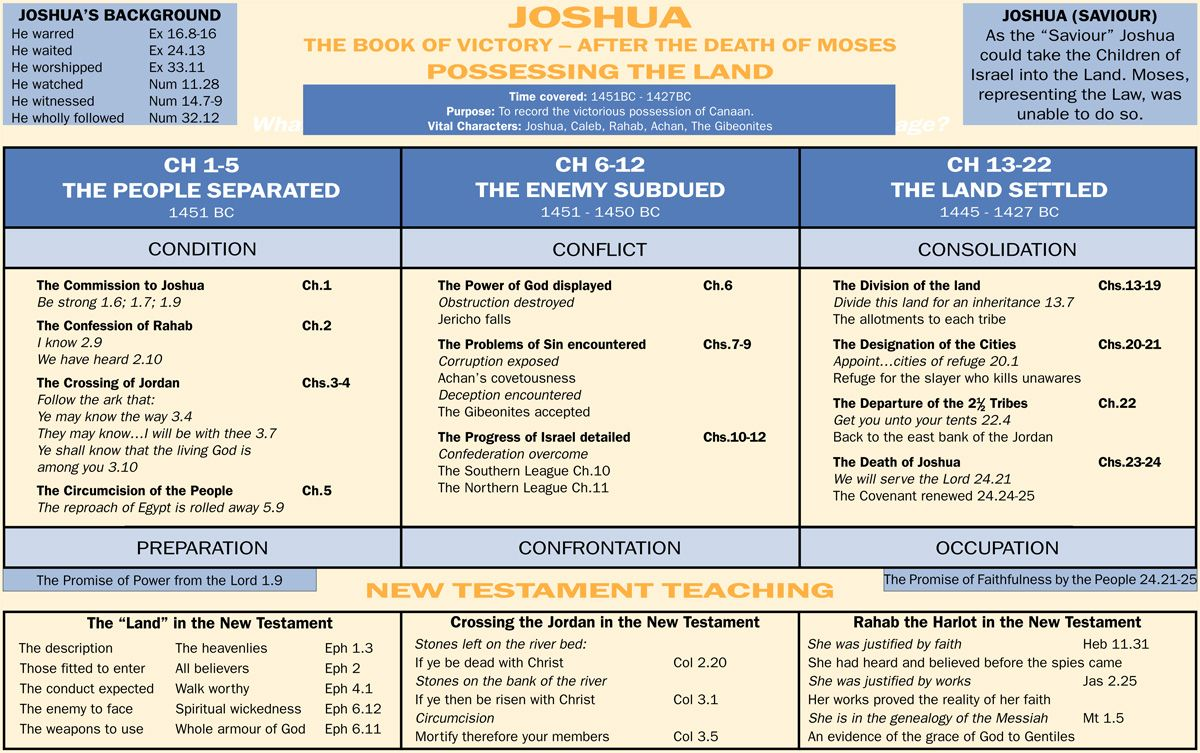
\includegraphics[scale=0.5, angle=90]{06OT-Joshua/References/2.JohnGrant-Joshua.jpg}
\caption[Joshua from John Grant]{Joshua from John Grant}
\label{fig:Joshua from John Grant}
\end{center}
\end{figure}

\newpage
\begin{figure}
\begin{center}
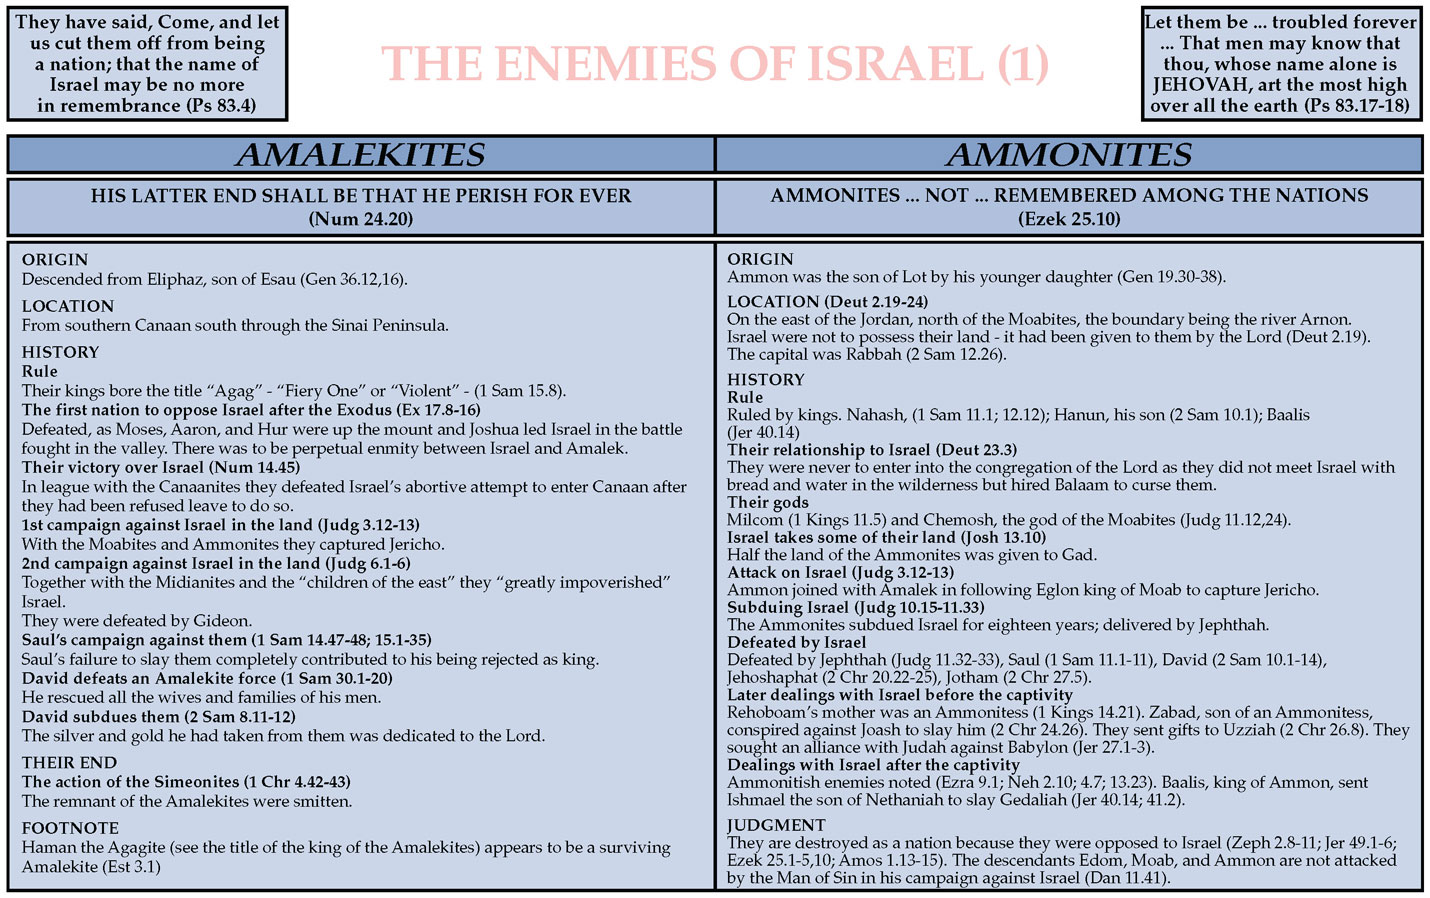
\includegraphics[scale=0.4, angle=90]{06OT-Joshua/References/3.EnemiesOfIsrael1.jpg}
\caption[Enemies of Israel 1]{Enemies of Israel 1}
\label{fig:Enemies of Israel 1}
\end{center}
\end{figure}

\newpage
\begin{figure}
\begin{center}
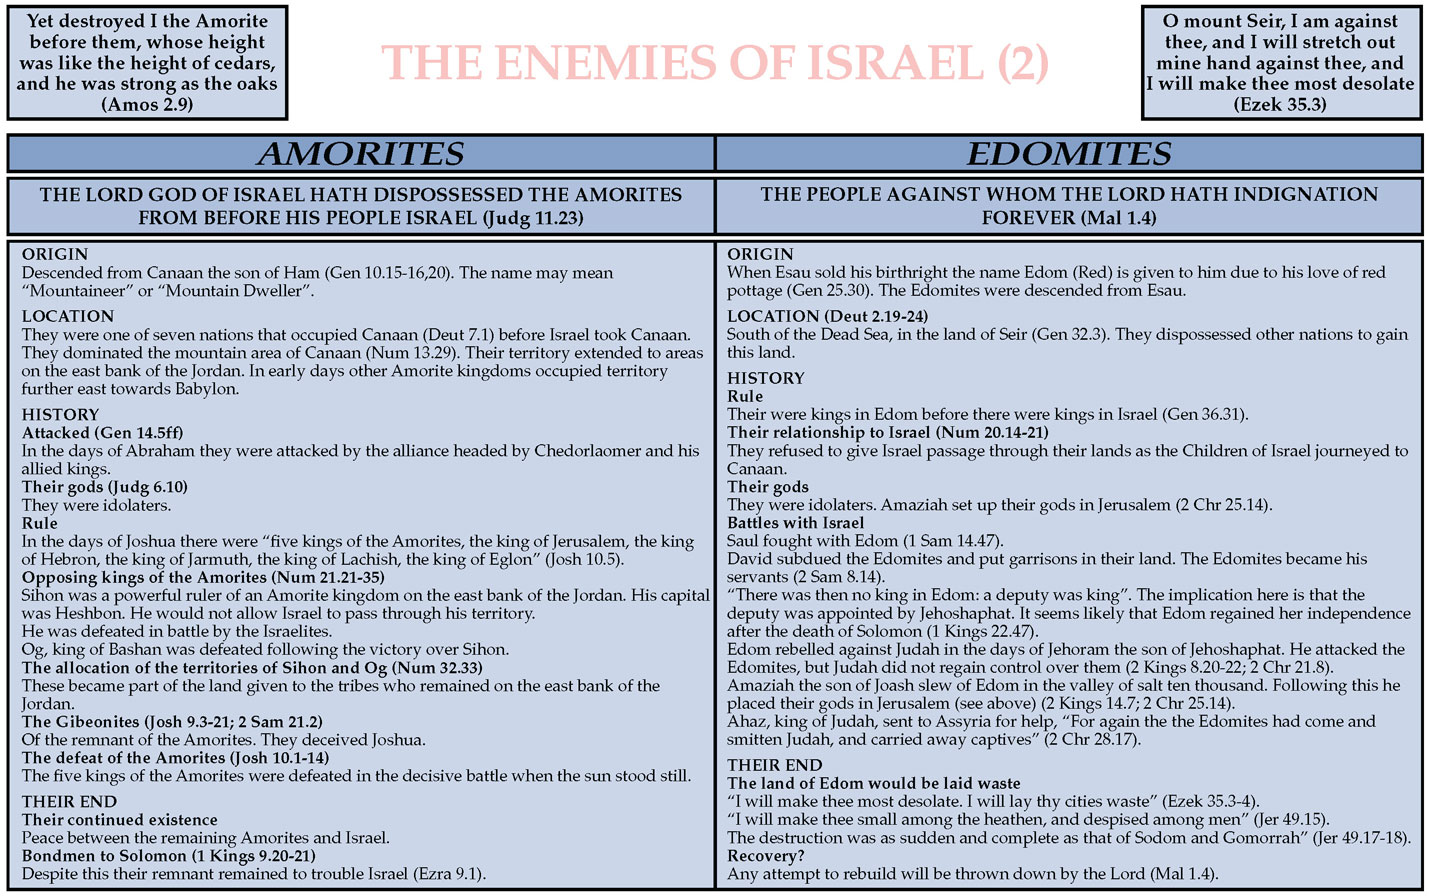
\includegraphics[scale=0.4, angle=90]{06OT-Joshua/References/4.EnemiesOfIsrael2.jpg}
\caption[Enemies of Israel 2]{Enemies of Israel 2}
\label{fig:Enemies of Israel 2}
\end{center}
\end{figure}

\newpage
\begin{figure}
\begin{center}
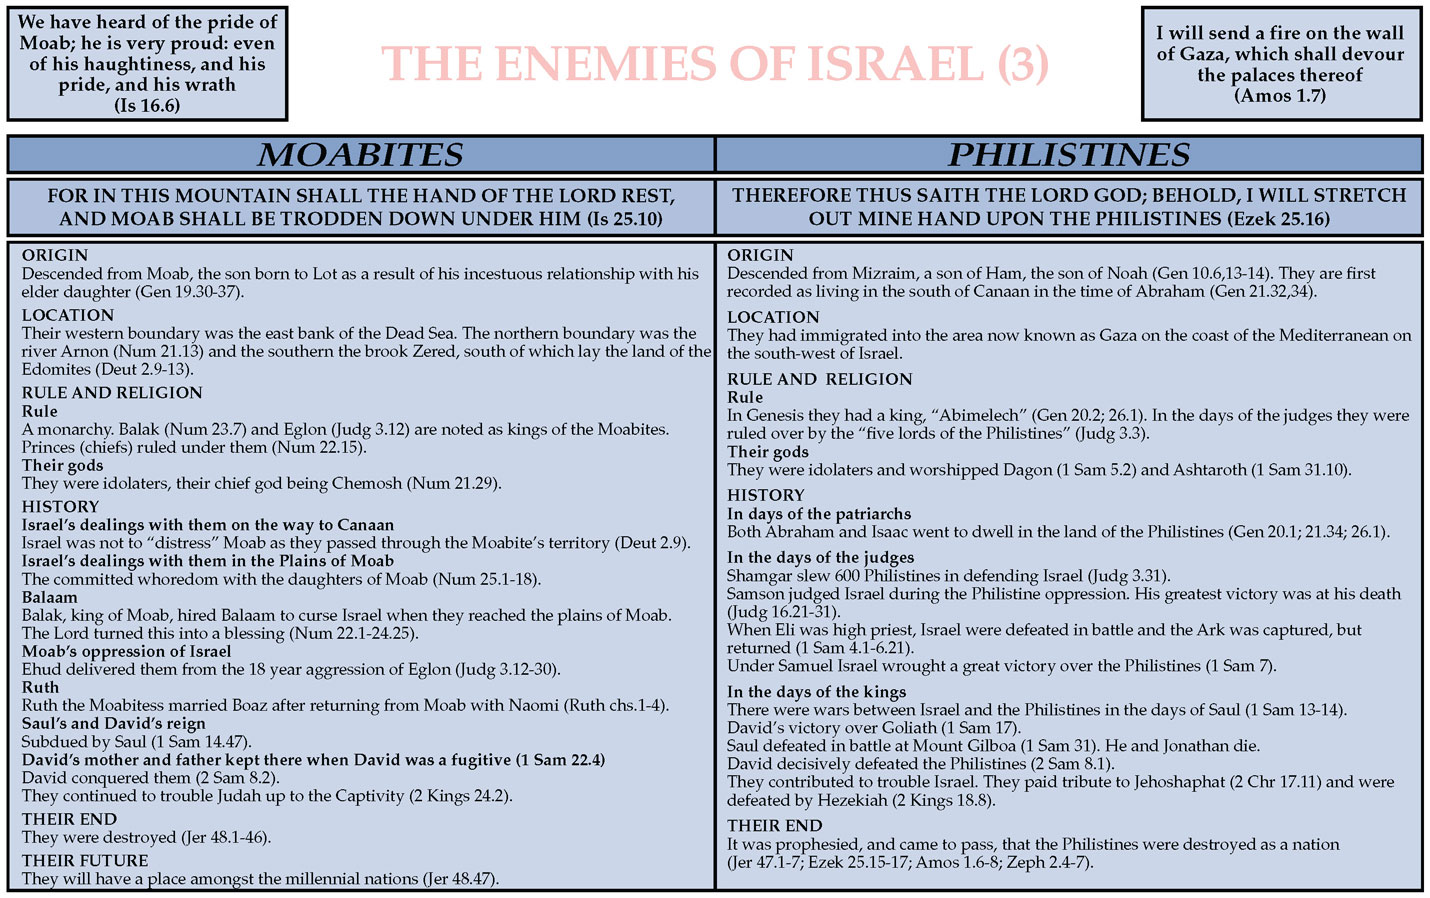
\includegraphics[scale=0.4, angle=90]{06OT-Joshua/References/5.EnemiesOfIsrael3.jpg}
\caption[Enemies of Israel 3]{Enemies of Israel 3}
\label{fig:Enemies of Israel 3}
\end{center}
\end{figure}

\newpage
\begin{figure}
\begin{center}
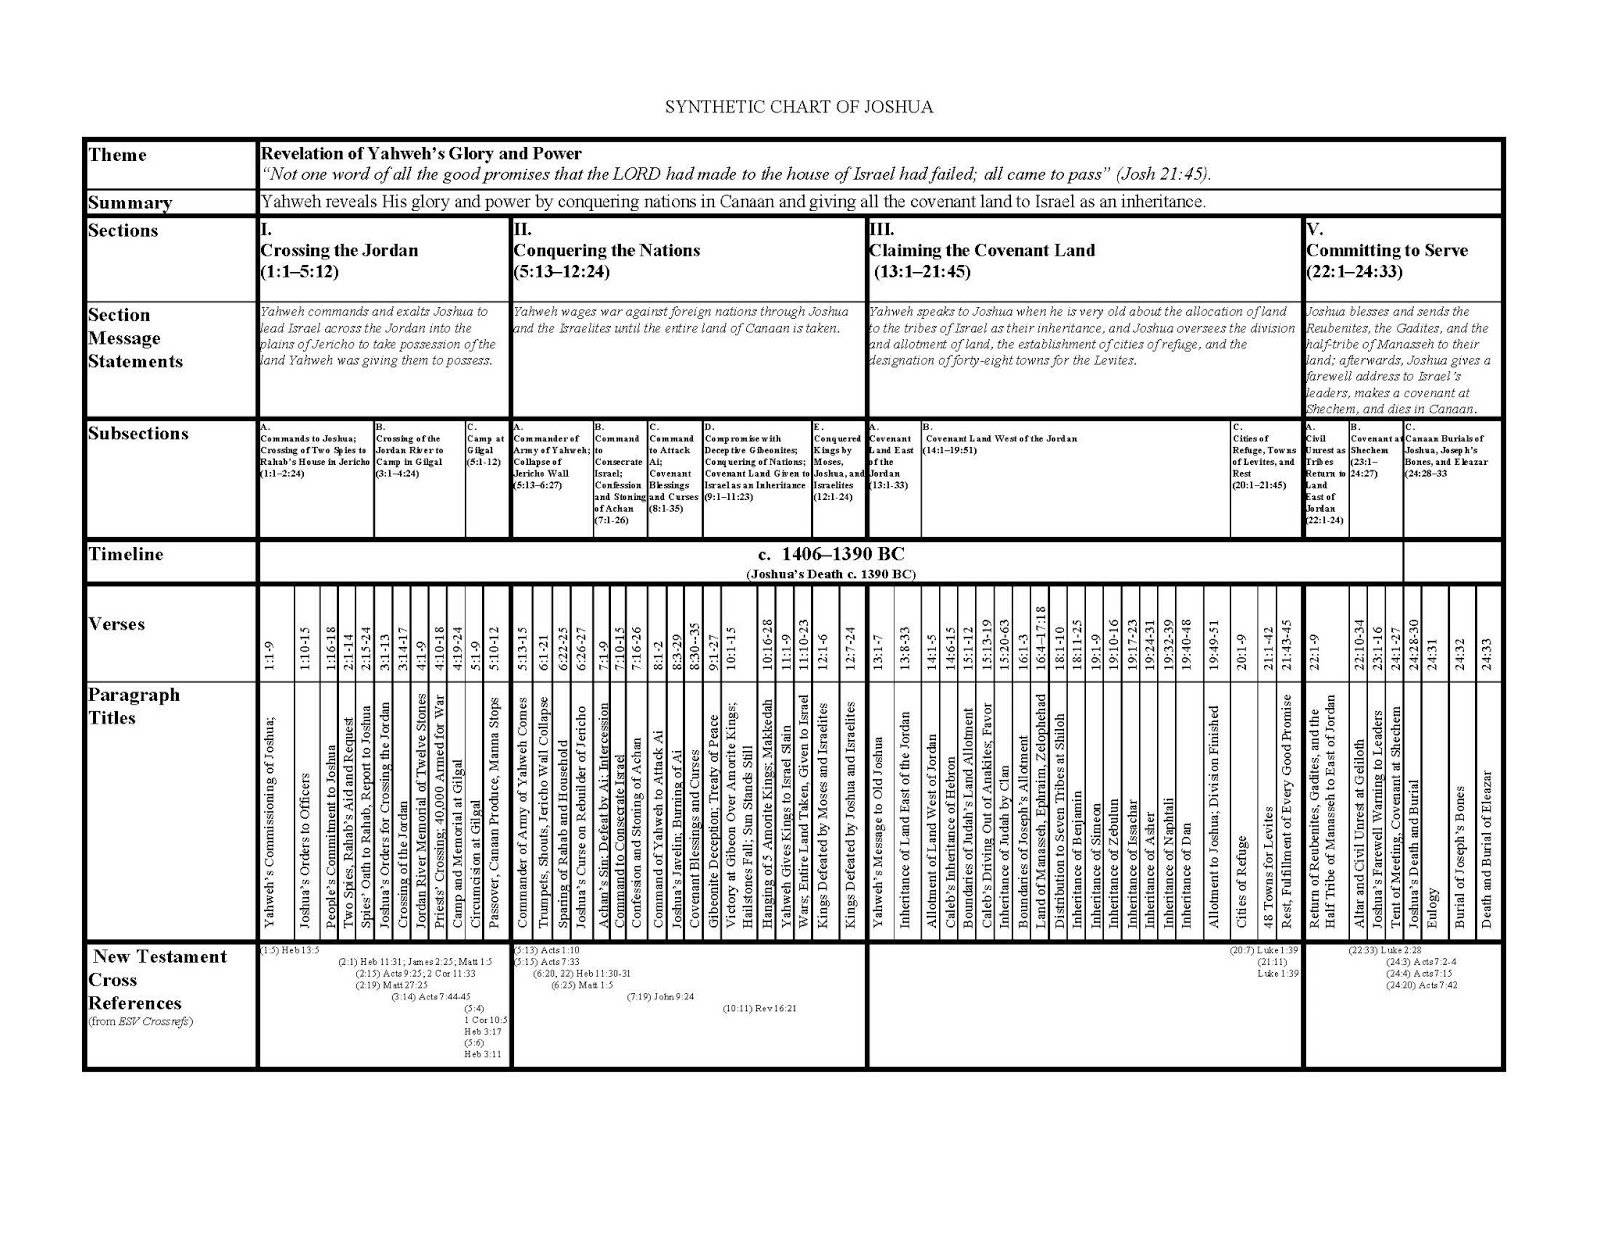
\includegraphics[scale=.4, angle=90]{06OT-Joshua/References/6.SyntheticChartofJoshua.jpg}
\caption[Synthetic Chart of Joshua]{Synthetic Chart of Joshua}
\label{fig:Synthetic Chart of Joshua}
\end{center}
\end{figure}


\newpage
\begin{figure}
\begin{center}
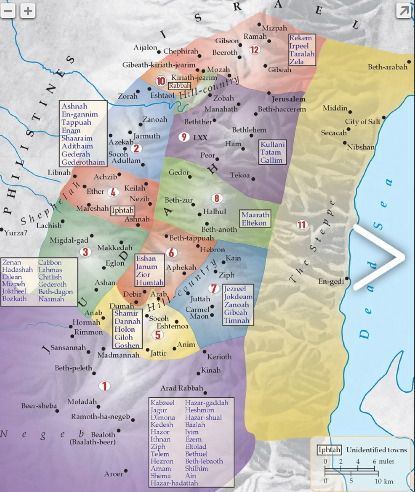
\includegraphics[scale=1, angle=0]{06OT-Joshua/References/7.WestSideOfDeadSea.jpg}
\caption[The West Side of the Dead Sea]{The West Side of the Dead Sea}
\label{fig:The West Side of the Dead Sea}
\end{center}
\end{figure}


\newpage
\begin{figure}
\begin{center}
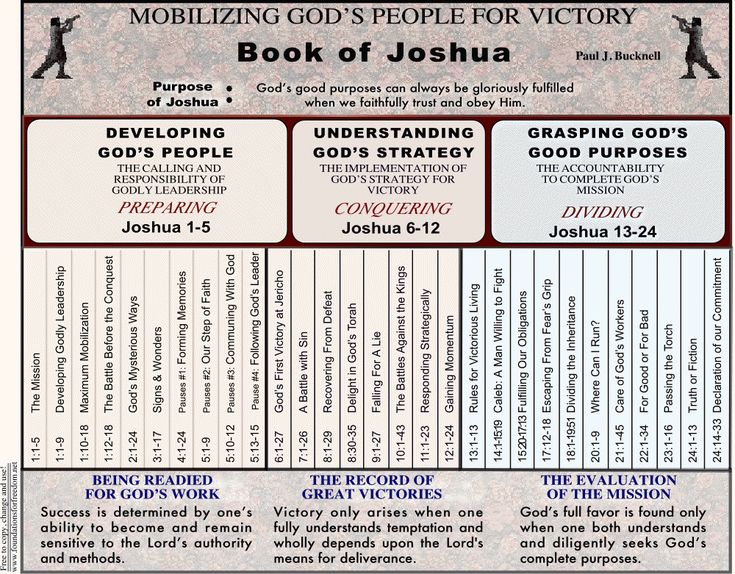
\includegraphics[scale=0.75, angle=90]{06OT-Joshua/References/8.Bucknell-Joshua.jpg}
\caption[Joshua from Bucknell]{Joshua from Bucknell}
\label{fig:Joshua from Bucknell}
\end{center}
\end{figure}


\newpage
\begin{figure}
\begin{center}
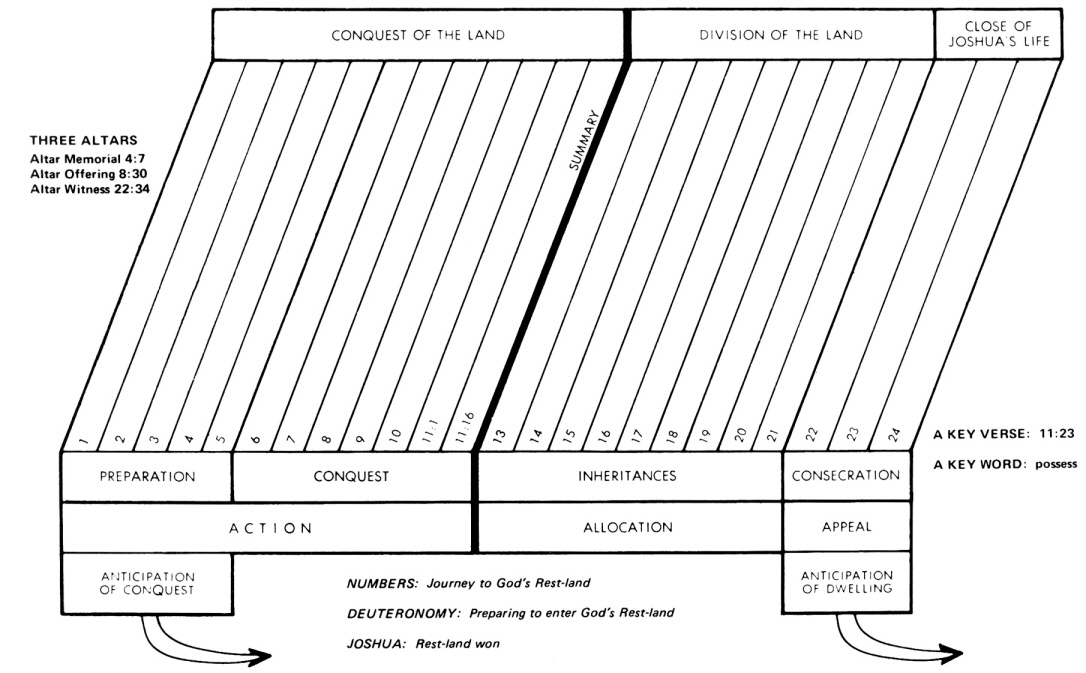
\includegraphics[scale=2, angle=90]{06OT-Joshua/References/9.Jensen-Joshua.png}
\caption[Joshua from Jensen]{Joshua from Jensen}
\label{fig:Joshua from Jensen}
\end{center}
\end{figure}


\newpage
\begin{figure}
\begin{center}
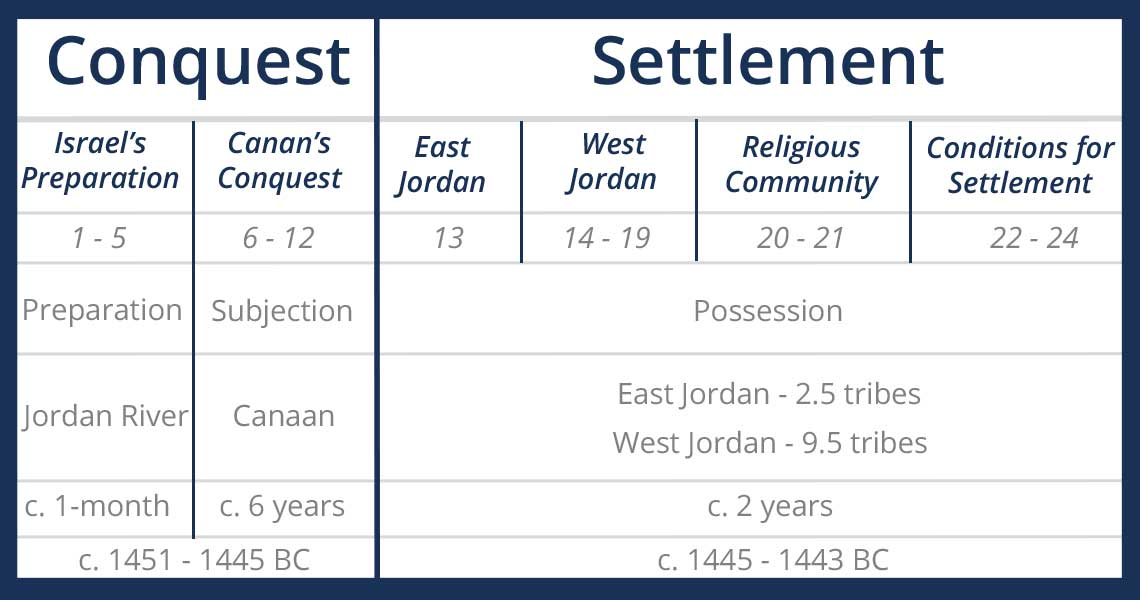
\includegraphics[scale=.5, angle=90]{06OT-Joshua/References/10.Bible-Brief-Joshua.jpg}
\caption[Bible Brief for Joshua]{Bible Brief for Joshua}
\label{fig:Bible Brief for Joshua}
\end{center}
\end{figure}

\newpage
\begin{figure}
\begin{center}
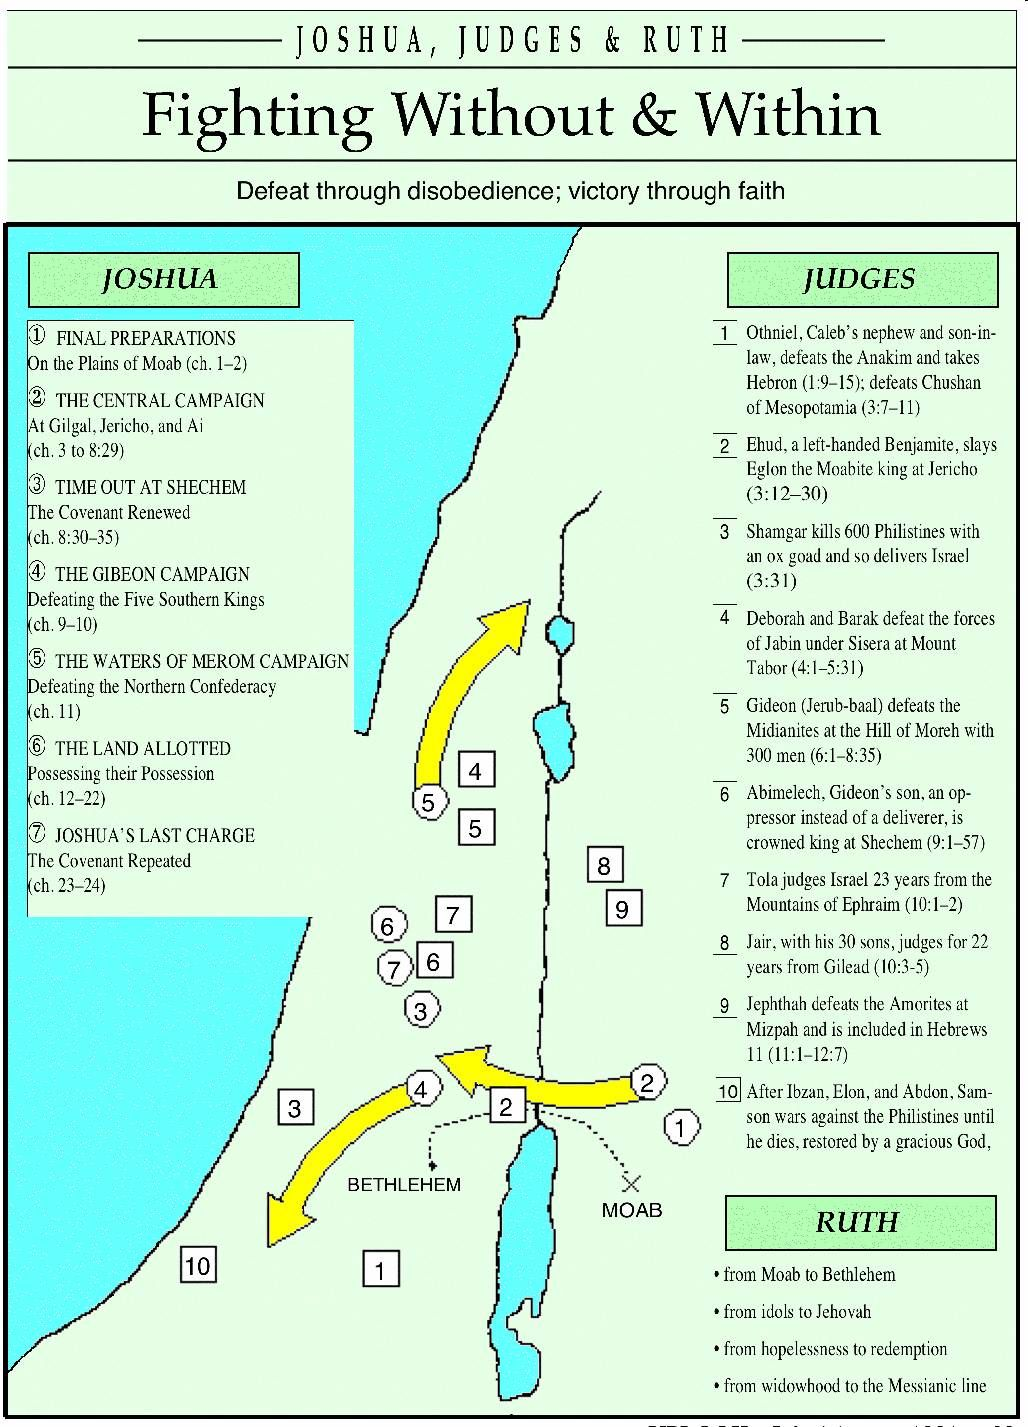
\includegraphics[scale=.5, angle=0]{06OT-Joshua/References/11.FightingInJoshuaAndJudges.jpg}
\caption[The Fighting in Joshua and Judges]{The Fighting in Joshua and Judges}
\label{fig:The Fighting in Joshua and Judges}
\end{center}
\end{figure}

\newpage
\begin{figure}
\begin{center}
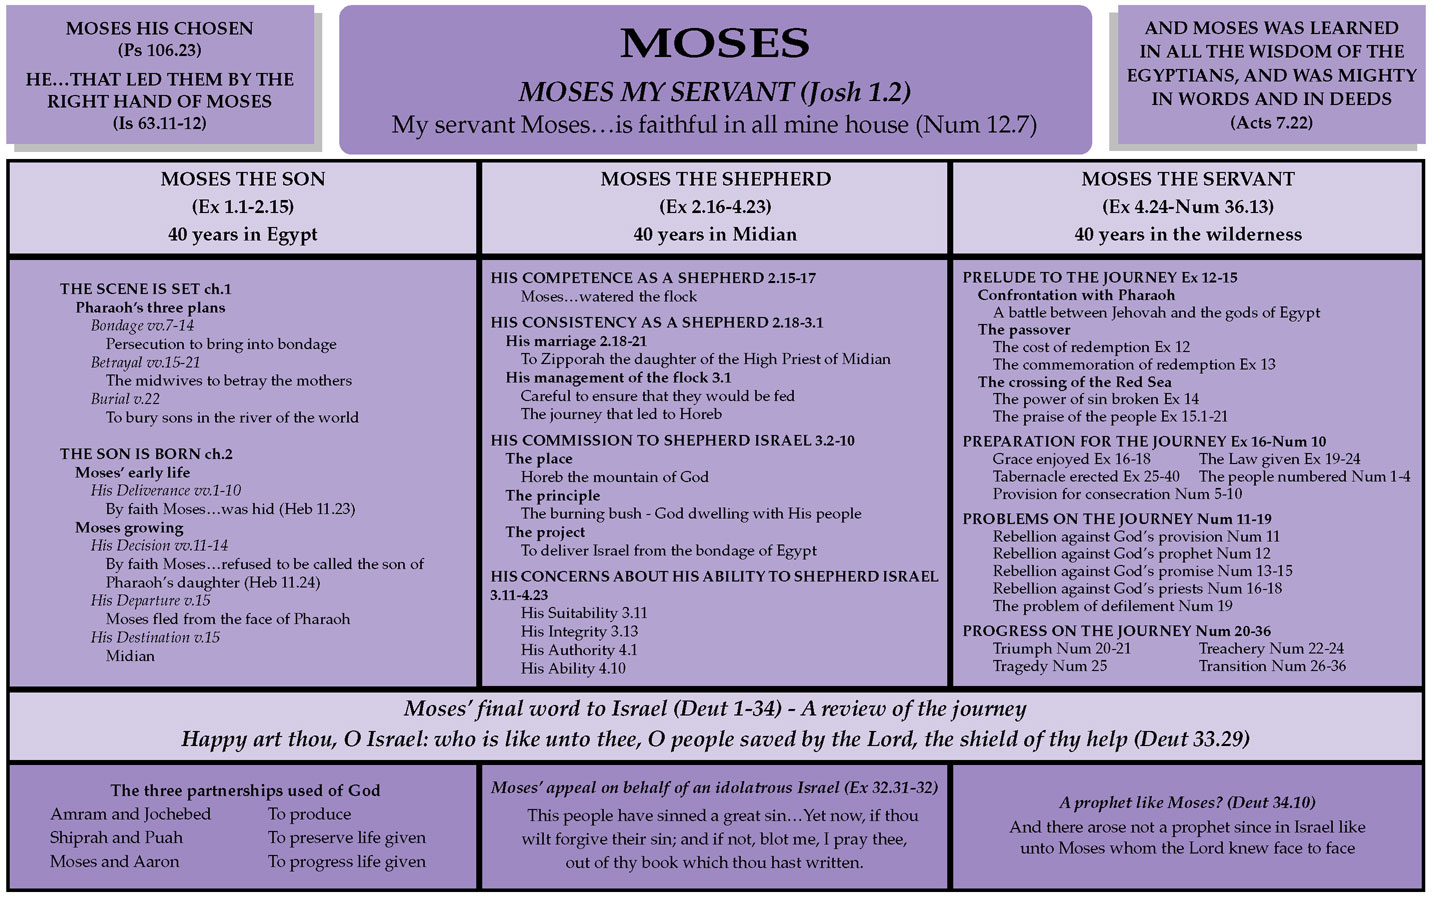
\includegraphics[scale=.4, angle=90]{06OT-Joshua/References/12.JohnGrantMoses.jpg}
\caption[Moses from John Grant]{Moses from John Grant}
\label{fig:Moses from John Grant}
\end{center}
\end{figure}








\chapter{Joshua 10}

\begin{figure}
  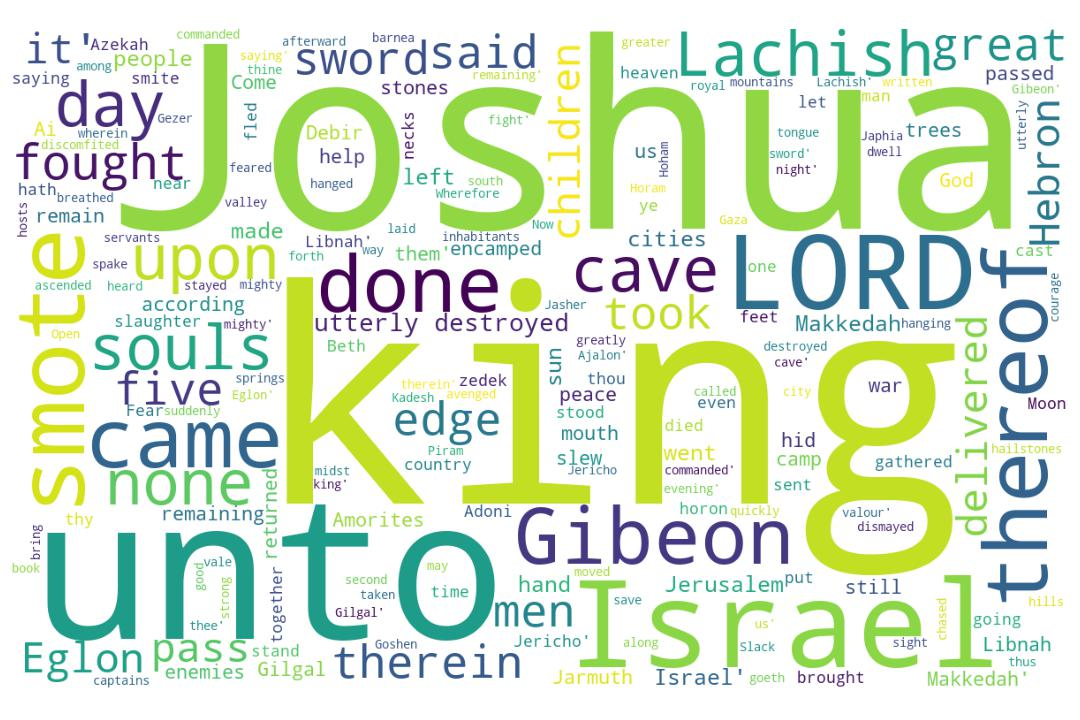
\includegraphics[width=\linewidth]{06OT-Joshua/Joshua10-WordCloud.jpg}
  \caption{Joshua 10 Word Cloud}
  \label{fig:Joshua 10 Word Cloud}
\end{figure}

\marginpar{\scriptsize \centering \fcolorbox{bone}{lime}{\textbf{THE SOUTHERN CAMPAIGN}}\\ (Joshua 10:1-43) \begin{compactenum}[I.][8]
	\item A \textbf{Strategic Advantage} \index[scripture]{Joshua!Jsh 10:01}  (Jsh 10:1) 
	\item \textbf{Solidarity} of the 5 enemy kings \index[scripture]{Joshua!Jsh 10:05}  (Jsh 10:5) 
	\item A \textbf{Surprise Attack} \index[scripture]{Joshua!Jsh 10:09}  (Jsh 10:9) 
	\item A \textbf{Slaughter} at Gibeon\index[scripture]{Joshua!Jsh 10:10}  (Jsh 10:10) 
	\item A \textbf{Stones} from heaven \index[scripture]{Joshua!Jsh 10:11}  (Jsh 10:11) 
	\item The \textbf{Stopping of the Sun} \index[scripture]{Joshua!Jsh 10:12--12}  (Jsh 10:12--13) 
	\item \textbf{Sealed} in a Cave \index[scripture]{Joshua!Jsh 10:18}  (Jsh 10:18) 
\end{compactenum}}



\footnote{\textcolor[cmyk]{0.99998,1,0,0}{\hyperlink{TOC}{Return to end of Table of Contents.}}}\footnote{\href{https://audiobible.com/bible/joshua_10.html}{\textcolor[cmyk]{0.99998,1,0,0}{Joshua 10 Audio}}}\textcolor[cmyk]{0.99998,1,0,0}{Now it came to pass, when Adoni-zedek king of Jerusalem had heard how Joshua had taken Ai, and had utterly destroyed it; as he had done to Jericho and her king, so he had done to Ai and her king; and how the inhabitants of Gibeon had made peace with Israel, and were among them;}
[2] \textcolor[cmyk]{0.99998,1,0,0}{That they feared greatly, because Gibeon \emph{was} a great city, as one of the royal cities, and because it \emph{was} greater than Ai, and all the men thereof \emph{were} mighty.}
[3] \textcolor[cmyk]{0.99998,1,0,0}{Wherefore Adoni-zedek king of Jerusalem sent unto Hoham king of Hebron, and unto Piram king of Jarmuth, and unto Japhia king of Lachish, and unto Debir king of Eglon, saying,}
[4] \textcolor[cmyk]{0.99998,1,0,0}{Come up unto me, and help me, that we may smite Gibeon: for it hath made peace with Joshua and with the children of Israel.}
[5] \textcolor[cmyk]{0.99998,1,0,0}{Therefore the five kings of the Amorites, \fcolorbox{bone}{bone}{the king of} Jerusalem, \fcolorbox{bone}{bone}{the king of} Hebron, \fcolorbox{bone}{bone}{the king of} Jarmuth, \fcolorbox{bone}{bone}{the king of} Lachish, \fcolorbox{bone}{bone}{the king of} Eglon, gathered themselves together, and went up, they and all their hosts, and encamped before Gibeon, and made war against it.}\\
\\
\P \textcolor[cmyk]{0.99998,1,0,0}{And the men of Gibeon sent unto Joshua to the camp to Gilgal, saying, Slack not thy hand from thy servants; come up to us quickly, and save us, and help us: for all the kings of the Amorites that dwell in the mountains are gathered together against us.}
[7] \textcolor[cmyk]{0.99998,1,0,0}{So Joshua ascended from Gilgal, he, and all the people of war with him, and all the mighty men of valour.}\\
\\
\P \textcolor[cmyk]{0.99998,1,0,0}{And the \fcolorbox{bone}{bone}{LORD} said unto Joshua, Fear them not: for I have delivered them into thine hand; there shall not a man of them stand before thee.}
[9] \textcolor[cmyk]{0.99998,1,0,0}{Joshua therefore came unto them suddenly, \emph{and} went up from Gilgal all night.}
[10] \textcolor[cmyk]{0.99998,1,0,0}{And the \fcolorbox{bone}{bone}{LORD} discomfited them before Israel, and slew them with a great slaughter at Gibeon, and chased them along the way that goeth up to Beth-horon, and smote them to Azekah, and unto Makkedah.}
[11] \textcolor[cmyk]{0.99998,1,0,0}{And it came to pass, as they fled from before Israel, \emph{and} were in the going down to Beth-horon, that the \fcolorbox{bone}{bone}{LORD} cast down great stones from heaven upon them unto Azekah, and they died: \emph{they} \emph{were} more which died with hailstones than \emph{they} whom the children of Israel slew with the sword.}\\
\\
\P \textcolor[cmyk]{0.99998,1,0,0}{Then spake Joshua to the \fcolorbox{bone}{bone}{LORD} in the day when the \fcolorbox{bone}{bone}{LORD} delivered up the Amorites before the children of Israel, and he said in the sight of Israel, Sun, stand thou still upon Gibeon; and thou, Moon, in the valley of Ajalon.}
[13] \textcolor[cmyk]{0.99998,1,0,0}{And the sun stood still, and the moon stayed, until the people had avenged themselves upon their enemies. \emph{Is} not this written in the book of Jasher? So the sun stood still in the midst of heaven, and hasted not to go down about a whole day.}
[14] \textcolor[cmyk]{0.99998,1,0,0}{And there was no day like that before it or after it, that the \fcolorbox{bone}{bone}{LORD} hearkened unto the voice of a man: for the \fcolorbox{bone}{bone}{LORD} fought for Israel.}\\
\\
\P \textcolor[cmyk]{0.99998,1,0,0}{And Joshua returned, and all Israel with him, unto the camp to Gilgal.}
[16] \textcolor[cmyk]{0.99998,1,0,0}{But these five kings fled, and hid themselves in a cave at Makkedah.}
[17] \textcolor[cmyk]{0.99998,1,0,0}{And it was told Joshua, saying, The five kings are found hid in a cave at Makkedah.}
[18] \textcolor[cmyk]{0.99998,1,0,0}{And Joshua said, Roll great stones upon the mouth of the cave, and set men by it for to keep them:}
[19] \textcolor[cmyk]{0.99998,1,0,0}{And stay ye not, \emph{but} pursue after your enemies, and smite the hindmost of them; suffer them not to enter into their cities: for the \fcolorbox{bone}{bone}{LORD} your God hath delivered them into your hand.}
[20] \textcolor[cmyk]{0.99998,1,0,0}{And it came to pass, when Joshua and the children of Israel had made an end of slaying them with a very great slaughter, till they were consumed, that the rest \emph{which} remained of them entered into fenced cities.}
[21] \textcolor[cmyk]{0.99998,1,0,0}{And all the people returned to the camp to Joshua at Makkedah in peace: none moved his tongue against any of the children of Israel.}
[22] \textcolor[cmyk]{0.99998,1,0,0}{Then said Joshua, Open the mouth of the cave, and bring out those five kings unto me out of the cave.}
[23] \textcolor[cmyk]{0.99998,1,0,0}{And they did so, and brought forth those five kings unto him out of the cave, \fcolorbox{bone}{bone}{the king of} Jerusalem, \fcolorbox{bone}{bone}{the king of} Hebron, \fcolorbox{bone}{bone}{the king of} Jarmuth, \fcolorbox{bone}{bone}{the king of} Lachish, \emph{and} \fcolorbox{bone}{bone}{the king of} Eglon.}
[24] \textcolor[cmyk]{0.99998,1,0,0}{And it came to pass, when they brought out those kings unto Joshua, that Joshua called for all the men of Israel, and said unto the captains of the men of war which went with him, Come near, put your feet upon the necks of these kings. And they came near, and put their feet upon the necks of them.}
[25] \textcolor[cmyk]{0.99998,1,0,0}{And Joshua said unto them, Fear not, nor be dismayed, be strong and of good courage: for thus shall the \fcolorbox{bone}{bone}{LORD} do to all your enemies against whom ye fight.}
[26] \textcolor[cmyk]{0.99998,1,0,0}{And afterward Joshua smote them, and slew them, and hanged them on five trees: and they were hanging upon the trees until the evening.}
[27] \textcolor[cmyk]{0.99998,1,0,0}{And it came to pass at the time of the going down of the sun, \emph{that} Joshua commanded, and they took them down off the trees, and cast them into the cave wherein they had been hid, and laid great stones in the cave's mouth, \emph{which} \emph{remain} until this very day.}\\
\\
\P \textcolor[cmyk]{0.99998,1,0,0}{And that day Joshua took Makkedah, and smote it with the edge of the sword, and the king thereof he utterly destroyed, them, and all the souls that \emph{were} therein; he let none remain: and he did to \fcolorbox{bone}{bone}{the king of} Makkedah as he did unto \fcolorbox{bone}{bone}{the king of} Jericho.}
[29] \textcolor[cmyk]{0.99998,1,0,0}{Then Joshua passed from Makkedah, and all Israel with him, unto Libnah, and fought against Libnah:}
[30] \textcolor[cmyk]{0.99998,1,0,0}{And the \fcolorbox{bone}{bone}{LORD} delivered it also, and the king thereof, into the hand of Israel; and he smote it with the edge of the sword, and all the souls that \emph{were} therein; he let none remain in it; but did unto the king thereof as he did unto \fcolorbox{bone}{bone}{the king of} Jericho.}\\
\\
\P \textcolor[cmyk]{0.99998,1,0,0}{And Joshua passed from Libnah, and all Israel with him, unto Lachish, and encamped against it, and fought against it:}
[32] \textcolor[cmyk]{0.99998,1,0,0}{And the \fcolorbox{bone}{bone}{LORD} delivered Lachish into the hand of Israel, which took it on the second day, and smote it with the edge of the sword, and all the souls that \emph{were} therein, according to all that he had done to Libnah.}\\
\\
\P \textcolor[cmyk]{0.99998,1,0,0}{Then Horam king of Gezer came up to help Lachish; and Joshua smote him and his people, until he had left him none remaining.}\\
\\
\P \textcolor[cmyk]{0.99998,1,0,0}{And from Lachish Joshua passed unto Eglon, and all Israel with him; and they encamped against it, and fought against it:}
[35] \textcolor[cmyk]{0.99998,1,0,0}{And they took it on that day, and smote it with the edge of the sword, and all the souls that \emph{were} therein he utterly destroyed that day, according to all that he had done to Lachish.}
[36] \textcolor[cmyk]{0.99998,1,0,0}{And Joshua went up from Eglon, and all Israel with him, unto Hebron; and they fought against it:}
[37] \textcolor[cmyk]{0.99998,1,0,0}{And they took it, and smote it with the edge of the sword, and the king thereof, and all the cities thereof, and all the souls that \emph{were} therein; he left none remaining, according to all that he had done to Eglon; but destroyed it utterly, and all the souls that \emph{were} therein.}\\
\\
\P \textcolor[cmyk]{0.99998,1,0,0}{And Joshua returned, and all Israel with him, to Debir; and fought against it:}
[39] \textcolor[cmyk]{0.99998,1,0,0}{And he took it, and the king thereof, and all the cities thereof; and they smote them with the edge of the sword, and utterly destroyed all the souls that \emph{were} therein; he left none remaining: as he had done to Hebron, so he did to Debir, and to the king thereof; as he had done also to Libnah, and to her king.}\\
\\
\P \textcolor[cmyk]{0.99998,1,0,0}{So Joshua smote all the country of the hills, and of the south, and of the vale, and of the springs, and all their kings: he left none remaining, but utterly destroyed all that breathed, as the \fcolorbox{bone}{bone}{LORD} God of Israel commanded.}
[41] \textcolor[cmyk]{0.99998,1,0,0}{And Joshua smote them from Kadesh-barnea even unto Gaza, and all the country of Goshen, even unto Gibeon.}
[42] \textcolor[cmyk]{0.99998,1,0,0}{And all these kings and their land did Joshua take at one time, because the \fcolorbox{bone}{bone}{LORD} God of Israel fought for Israel.}
[43] \textcolor[cmyk]{0.99998,1,0,0}{And Joshua returned, and all Israel with him, unto the camp to Gilgal.}

\index[NWIV]{55!Joshua!Jos 10:1}\index[AWIP]{Now!Joshua!Jos 10:1}\index[AWIP]{it!Joshua!Jos 10:1}\index[AWIP]{it!Joshua!Jos 10:1 (2)}\index[AWIP]{came!Joshua!Jos 10:1}\index[AWIP]{to!Joshua!Jos 10:1}\index[AWIP]{to!Joshua!Jos 10:1 (2)}\index[AWIP]{to!Joshua!Jos 10:1 (3)}\index[AWIP]{pass!Joshua!Jos 10:1}\index[AWIP]{when!Joshua!Jos 10:1}\index[AWIP]{Adoni-zedek!Joshua!Jos 10:1}\index[AWIP]{king!Joshua!Jos 10:1}\index[AWIP]{king!Joshua!Jos 10:1 (2)}\index[AWIP]{king!Joshua!Jos 10:1 (3)}\index[AWIP]{of!Joshua!Jos 10:1}\index[AWIP]{of!Joshua!Jos 10:1 (2)}\index[AWIP]{Jerusalem!Joshua!Jos 10:1}\index[AWIP]{had!Joshua!Jos 10:1}\index[AWIP]{had!Joshua!Jos 10:1 (2)}\index[AWIP]{had!Joshua!Jos 10:1 (3)}\index[AWIP]{had!Joshua!Jos 10:1 (4)}\index[AWIP]{had!Joshua!Jos 10:1 (5)}\index[AWIP]{had!Joshua!Jos 10:1 (6)}\index[AWIP]{heard!Joshua!Jos 10:1}\index[AWIP]{how!Joshua!Jos 10:1}\index[AWIP]{how!Joshua!Jos 10:1 (2)}\index[AWIP]{Joshua!Joshua!Jos 10:1}\index[AWIP]{taken!Joshua!Jos 10:1}\index[AWIP]{Ai!Joshua!Jos 10:1}\index[AWIP]{Ai!Joshua!Jos 10:1 (2)}\index[AWIP]{and!Joshua!Jos 10:1}\index[AWIP]{and!Joshua!Jos 10:1 (2)}\index[AWIP]{and!Joshua!Jos 10:1 (3)}\index[AWIP]{and!Joshua!Jos 10:1 (4)}\index[AWIP]{and!Joshua!Jos 10:1 (5)}\index[AWIP]{utterly!Joshua!Jos 10:1}\index[AWIP]{destroyed!Joshua!Jos 10:1}\index[AWIP]{as!Joshua!Jos 10:1}\index[AWIP]{he!Joshua!Jos 10:1}\index[AWIP]{he!Joshua!Jos 10:1 (2)}\index[AWIP]{done!Joshua!Jos 10:1}\index[AWIP]{done!Joshua!Jos 10:1 (2)}\index[AWIP]{Jericho!Joshua!Jos 10:1}\index[AWIP]{her!Joshua!Jos 10:1}\index[AWIP]{her!Joshua!Jos 10:1 (2)}\index[AWIP]{so!Joshua!Jos 10:1}\index[AWIP]{the!Joshua!Jos 10:1}\index[AWIP]{inhabitants!Joshua!Jos 10:1}\index[AWIP]{Gibeon!Joshua!Jos 10:1}\index[AWIP]{made!Joshua!Jos 10:1}\index[AWIP]{peace!Joshua!Jos 10:1}\index[AWIP]{with!Joshua!Jos 10:1}\index[AWIP]{Israel!Joshua!Jos 10:1}\index[AWIP]{were!Joshua!Jos 10:1}\index[AWIP]{among!Joshua!Jos 10:1}\index[AWIP]{them!Joshua!Jos 10:1}

\index[NWIV]{30!Joshua!Jos 10:2}\index[AWIP]{That!Joshua!Jos 10:2}\index[AWIP]{they!Joshua!Jos 10:2}\index[AWIP]{feared!Joshua!Jos 10:2}\index[AWIP]{greatly!Joshua!Jos 10:2}\index[AWIP]{because!Joshua!Jos 10:2}\index[AWIP]{because!Joshua!Jos 10:2 (2)}\index[AWIP]{Gibeon!Joshua!Jos 10:2}\index[AWIP]{\emph{was}!Joshua!Jos 10:2}\index[AWIP]{\emph{was}!Joshua!Jos 10:2 (2)}\index[AWIP]{a!Joshua!Jos 10:2}\index[AWIP]{great!Joshua!Jos 10:2}\index[AWIP]{city!Joshua!Jos 10:2}\index[AWIP]{as!Joshua!Jos 10:2}\index[AWIP]{one!Joshua!Jos 10:2}\index[AWIP]{of!Joshua!Jos 10:2}\index[AWIP]{the!Joshua!Jos 10:2}\index[AWIP]{the!Joshua!Jos 10:2 (2)}\index[AWIP]{royal!Joshua!Jos 10:2}\index[AWIP]{cities!Joshua!Jos 10:2}\index[AWIP]{and!Joshua!Jos 10:2}\index[AWIP]{and!Joshua!Jos 10:2 (2)}\index[AWIP]{it!Joshua!Jos 10:2}\index[AWIP]{greater!Joshua!Jos 10:2}\index[AWIP]{than!Joshua!Jos 10:2}\index[AWIP]{Ai!Joshua!Jos 10:2}\index[AWIP]{all!Joshua!Jos 10:2}\index[AWIP]{men!Joshua!Jos 10:2}\index[AWIP]{thereof!Joshua!Jos 10:2}\index[AWIP]{\emph{were}!Joshua!Jos 10:2}\index[AWIP]{mighty!Joshua!Jos 10:2}\index[AWIP]{\emph{was}!Joshua!Jos 10:2}\index[AWIP]{\emph{was}!Joshua!Jos 10:2 (2)}\index[AWIP]{\emph{were}!Joshua!Jos 10:2}

\index[NWIV]{30!Joshua!Jos 10:3}\index[AWIP]{Wherefore!Joshua!Jos 10:3}\index[AWIP]{Adoni-zedek!Joshua!Jos 10:3}\index[AWIP]{king!Joshua!Jos 10:3}\index[AWIP]{king!Joshua!Jos 10:3 (2)}\index[AWIP]{king!Joshua!Jos 10:3 (3)}\index[AWIP]{king!Joshua!Jos 10:3 (4)}\index[AWIP]{king!Joshua!Jos 10:3 (5)}\index[AWIP]{of!Joshua!Jos 10:3}\index[AWIP]{of!Joshua!Jos 10:3 (2)}\index[AWIP]{of!Joshua!Jos 10:3 (3)}\index[AWIP]{of!Joshua!Jos 10:3 (4)}\index[AWIP]{of!Joshua!Jos 10:3 (5)}\index[AWIP]{Jerusalem!Joshua!Jos 10:3}\index[AWIP]{sent!Joshua!Jos 10:3}\index[AWIP]{unto!Joshua!Jos 10:3}\index[AWIP]{unto!Joshua!Jos 10:3 (2)}\index[AWIP]{unto!Joshua!Jos 10:3 (3)}\index[AWIP]{unto!Joshua!Jos 10:3 (4)}\index[AWIP]{Hoham!Joshua!Jos 10:3}\index[AWIP]{Hebron!Joshua!Jos 10:3}\index[AWIP]{and!Joshua!Jos 10:3}\index[AWIP]{and!Joshua!Jos 10:3 (2)}\index[AWIP]{and!Joshua!Jos 10:3 (3)}\index[AWIP]{Piram!Joshua!Jos 10:3}\index[AWIP]{Jarmuth!Joshua!Jos 10:3}\index[AWIP]{Japhia!Joshua!Jos 10:3}\index[AWIP]{Lachish!Joshua!Jos 10:3}\index[AWIP]{Debir!Joshua!Jos 10:3}\index[AWIP]{Eglon!Joshua!Jos 10:3}\index[AWIP]{saying!Joshua!Jos 10:3}

\index[NWIV]{25!Joshua!Jos 10:4}\index[AWIP]{Come!Joshua!Jos 10:4}\index[AWIP]{up!Joshua!Jos 10:4}\index[AWIP]{unto!Joshua!Jos 10:4}\index[AWIP]{me!Joshua!Jos 10:4}\index[AWIP]{me!Joshua!Jos 10:4 (2)}\index[AWIP]{and!Joshua!Jos 10:4}\index[AWIP]{and!Joshua!Jos 10:4 (2)}\index[AWIP]{help!Joshua!Jos 10:4}\index[AWIP]{that!Joshua!Jos 10:4}\index[AWIP]{we!Joshua!Jos 10:4}\index[AWIP]{may!Joshua!Jos 10:4}\index[AWIP]{smite!Joshua!Jos 10:4}\index[AWIP]{Gibeon!Joshua!Jos 10:4}\index[AWIP]{for!Joshua!Jos 10:4}\index[AWIP]{it!Joshua!Jos 10:4}\index[AWIP]{hath!Joshua!Jos 10:4}\index[AWIP]{made!Joshua!Jos 10:4}\index[AWIP]{peace!Joshua!Jos 10:4}\index[AWIP]{with!Joshua!Jos 10:4}\index[AWIP]{with!Joshua!Jos 10:4 (2)}\index[AWIP]{Joshua!Joshua!Jos 10:4}\index[AWIP]{the!Joshua!Jos 10:4}\index[AWIP]{children!Joshua!Jos 10:4}\index[AWIP]{of!Joshua!Jos 10:4}\index[AWIP]{Israel!Joshua!Jos 10:4}

\index[NWIV]{47!Joshua!Jos 10:5}\index[AWIP]{Therefore!Joshua!Jos 10:5}\index[AWIP]{the!Joshua!Jos 10:5}\index[AWIP]{the!Joshua!Jos 10:5 (2)}\index[AWIP]{the!Joshua!Jos 10:5 (3)}\index[AWIP]{the!Joshua!Jos 10:5 (4)}\index[AWIP]{the!Joshua!Jos 10:5 (5)}\index[AWIP]{the!Joshua!Jos 10:5 (6)}\index[AWIP]{the!Joshua!Jos 10:5 (7)}\index[AWIP]{five!Joshua!Jos 10:5}\index[AWIP]{kings!Joshua!Jos 10:5}\index[AWIP]{of!Joshua!Jos 10:5}\index[AWIP]{of!Joshua!Jos 10:5 (2)}\index[AWIP]{of!Joshua!Jos 10:5 (3)}\index[AWIP]{of!Joshua!Jos 10:5 (4)}\index[AWIP]{of!Joshua!Jos 10:5 (5)}\index[AWIP]{of!Joshua!Jos 10:5 (6)}\index[AWIP]{Amorites!Joshua!Jos 10:5}\index[AWIP]{king!Joshua!Jos 10:5}\index[AWIP]{king!Joshua!Jos 10:5 (2)}\index[AWIP]{king!Joshua!Jos 10:5 (3)}\index[AWIP]{king!Joshua!Jos 10:5 (4)}\index[AWIP]{king!Joshua!Jos 10:5 (5)}\index[AWIP]{Jerusalem!Joshua!Jos 10:5}\index[AWIP]{Hebron!Joshua!Jos 10:5}\index[AWIP]{Jarmuth!Joshua!Jos 10:5}\index[AWIP]{Lachish!Joshua!Jos 10:5}\index[AWIP]{Eglon!Joshua!Jos 10:5}\index[AWIP]{gathered!Joshua!Jos 10:5}\index[AWIP]{themselves!Joshua!Jos 10:5}\index[AWIP]{together!Joshua!Jos 10:5}\index[AWIP]{and!Joshua!Jos 10:5}\index[AWIP]{and!Joshua!Jos 10:5 (2)}\index[AWIP]{and!Joshua!Jos 10:5 (3)}\index[AWIP]{and!Joshua!Jos 10:5 (4)}\index[AWIP]{went!Joshua!Jos 10:5}\index[AWIP]{up!Joshua!Jos 10:5}\index[AWIP]{they!Joshua!Jos 10:5}\index[AWIP]{all!Joshua!Jos 10:5}\index[AWIP]{their!Joshua!Jos 10:5}\index[AWIP]{hosts!Joshua!Jos 10:5}\index[AWIP]{encamped!Joshua!Jos 10:5}\index[AWIP]{before!Joshua!Jos 10:5}\index[AWIP]{Gibeon!Joshua!Jos 10:5}\index[AWIP]{made!Joshua!Jos 10:5}\index[AWIP]{war!Joshua!Jos 10:5}\index[AWIP]{against!Joshua!Jos 10:5}\index[AWIP]{it!Joshua!Jos 10:5}

\index[NWIV]{49!Joshua!Jos 10:6}\index[AWIP]{And!Joshua!Jos 10:6}\index[AWIP]{the!Joshua!Jos 10:6}\index[AWIP]{the!Joshua!Jos 10:6 (2)}\index[AWIP]{the!Joshua!Jos 10:6 (3)}\index[AWIP]{the!Joshua!Jos 10:6 (4)}\index[AWIP]{the!Joshua!Jos 10:6 (5)}\index[AWIP]{men!Joshua!Jos 10:6}\index[AWIP]{of!Joshua!Jos 10:6}\index[AWIP]{of!Joshua!Jos 10:6 (2)}\index[AWIP]{Gibeon!Joshua!Jos 10:6}\index[AWIP]{sent!Joshua!Jos 10:6}\index[AWIP]{unto!Joshua!Jos 10:6}\index[AWIP]{Joshua!Joshua!Jos 10:6}\index[AWIP]{to!Joshua!Jos 10:6}\index[AWIP]{to!Joshua!Jos 10:6 (2)}\index[AWIP]{to!Joshua!Jos 10:6 (3)}\index[AWIP]{camp!Joshua!Jos 10:6}\index[AWIP]{Gilgal!Joshua!Jos 10:6}\index[AWIP]{saying!Joshua!Jos 10:6}\index[AWIP]{Slack!Joshua!Jos 10:6}\index[AWIP]{not!Joshua!Jos 10:6}\index[AWIP]{thy!Joshua!Jos 10:6}\index[AWIP]{thy!Joshua!Jos 10:6 (2)}\index[AWIP]{hand!Joshua!Jos 10:6}\index[AWIP]{from!Joshua!Jos 10:6}\index[AWIP]{servants!Joshua!Jos 10:6}\index[AWIP]{come!Joshua!Jos 10:6}\index[AWIP]{up!Joshua!Jos 10:6}\index[AWIP]{us!Joshua!Jos 10:6}\index[AWIP]{us!Joshua!Jos 10:6 (2)}\index[AWIP]{us!Joshua!Jos 10:6 (3)}\index[AWIP]{us!Joshua!Jos 10:6 (4)}\index[AWIP]{quickly!Joshua!Jos 10:6}\index[AWIP]{and!Joshua!Jos 10:6}\index[AWIP]{and!Joshua!Jos 10:6 (2)}\index[AWIP]{save!Joshua!Jos 10:6}\index[AWIP]{help!Joshua!Jos 10:6}\index[AWIP]{for!Joshua!Jos 10:6}\index[AWIP]{all!Joshua!Jos 10:6}\index[AWIP]{kings!Joshua!Jos 10:6}\index[AWIP]{Amorites!Joshua!Jos 10:6}\index[AWIP]{that!Joshua!Jos 10:6}\index[AWIP]{dwell!Joshua!Jos 10:6}\index[AWIP]{in!Joshua!Jos 10:6}\index[AWIP]{mountains!Joshua!Jos 10:6}\index[AWIP]{are!Joshua!Jos 10:6}\index[AWIP]{gathered!Joshua!Jos 10:6}\index[AWIP]{together!Joshua!Jos 10:6}\index[AWIP]{against!Joshua!Jos 10:6}

\index[NWIV]{21!Joshua!Jos 10:7}\index[AWIP]{So!Joshua!Jos 10:7}\index[AWIP]{Joshua!Joshua!Jos 10:7}\index[AWIP]{ascended!Joshua!Jos 10:7}\index[AWIP]{from!Joshua!Jos 10:7}\index[AWIP]{Gilgal!Joshua!Jos 10:7}\index[AWIP]{he!Joshua!Jos 10:7}\index[AWIP]{and!Joshua!Jos 10:7}\index[AWIP]{and!Joshua!Jos 10:7 (2)}\index[AWIP]{all!Joshua!Jos 10:7}\index[AWIP]{all!Joshua!Jos 10:7 (2)}\index[AWIP]{the!Joshua!Jos 10:7}\index[AWIP]{the!Joshua!Jos 10:7 (2)}\index[AWIP]{people!Joshua!Jos 10:7}\index[AWIP]{of!Joshua!Jos 10:7}\index[AWIP]{of!Joshua!Jos 10:7 (2)}\index[AWIP]{war!Joshua!Jos 10:7}\index[AWIP]{with!Joshua!Jos 10:7}\index[AWIP]{him!Joshua!Jos 10:7}\index[AWIP]{mighty!Joshua!Jos 10:7}\index[AWIP]{men!Joshua!Jos 10:7}\index[AWIP]{valour!Joshua!Jos 10:7}

\index[NWIV]{27!Joshua!Jos 10:8}\index[AWIP]{And!Joshua!Jos 10:8}\index[AWIP]{the!Joshua!Jos 10:8}\index[AWIP]{LORD!Joshua!Jos 10:8}\index[AWIP]{said!Joshua!Jos 10:8}\index[AWIP]{unto!Joshua!Jos 10:8}\index[AWIP]{Joshua!Joshua!Jos 10:8}\index[AWIP]{Fear!Joshua!Jos 10:8}\index[AWIP]{them!Joshua!Jos 10:8}\index[AWIP]{them!Joshua!Jos 10:8 (2)}\index[AWIP]{them!Joshua!Jos 10:8 (3)}\index[AWIP]{not!Joshua!Jos 10:8}\index[AWIP]{not!Joshua!Jos 10:8 (2)}\index[AWIP]{for!Joshua!Jos 10:8}\index[AWIP]{I!Joshua!Jos 10:8}\index[AWIP]{have!Joshua!Jos 10:8}\index[AWIP]{delivered!Joshua!Jos 10:8}\index[AWIP]{into!Joshua!Jos 10:8}\index[AWIP]{thine!Joshua!Jos 10:8}\index[AWIP]{hand!Joshua!Jos 10:8}\index[AWIP]{there!Joshua!Jos 10:8}\index[AWIP]{shall!Joshua!Jos 10:8}\index[AWIP]{a!Joshua!Jos 10:8}\index[AWIP]{man!Joshua!Jos 10:8}\index[AWIP]{of!Joshua!Jos 10:8}\index[AWIP]{stand!Joshua!Jos 10:8}\index[AWIP]{before!Joshua!Jos 10:8}\index[AWIP]{thee!Joshua!Jos 10:8}

\index[NWIV]{13!Joshua!Jos 10:9}\index[AWIP]{Joshua!Joshua!Jos 10:9}\index[AWIP]{therefore!Joshua!Jos 10:9}\index[AWIP]{came!Joshua!Jos 10:9}\index[AWIP]{unto!Joshua!Jos 10:9}\index[AWIP]{them!Joshua!Jos 10:9}\index[AWIP]{suddenly!Joshua!Jos 10:9}\index[AWIP]{\emph{and}!Joshua!Jos 10:9}\index[AWIP]{went!Joshua!Jos 10:9}\index[AWIP]{up!Joshua!Jos 10:9}\index[AWIP]{from!Joshua!Jos 10:9}\index[AWIP]{Gilgal!Joshua!Jos 10:9}\index[AWIP]{all!Joshua!Jos 10:9}\index[AWIP]{night!Joshua!Jos 10:9}\index[AWIP]{\emph{and}!Joshua!Jos 10:9}

\index[NWIV]{35!Joshua!Jos 10:10}\index[AWIP]{And!Joshua!Jos 10:10}\index[AWIP]{the!Joshua!Jos 10:10}\index[AWIP]{the!Joshua!Jos 10:10 (2)}\index[AWIP]{LORD!Joshua!Jos 10:10}\index[AWIP]{discomfited!Joshua!Jos 10:10}\index[AWIP]{them!Joshua!Jos 10:10}\index[AWIP]{them!Joshua!Jos 10:10 (2)}\index[AWIP]{them!Joshua!Jos 10:10 (3)}\index[AWIP]{them!Joshua!Jos 10:10 (4)}\index[AWIP]{before!Joshua!Jos 10:10}\index[AWIP]{Israel!Joshua!Jos 10:10}\index[AWIP]{and!Joshua!Jos 10:10}\index[AWIP]{and!Joshua!Jos 10:10 (2)}\index[AWIP]{and!Joshua!Jos 10:10 (3)}\index[AWIP]{and!Joshua!Jos 10:10 (4)}\index[AWIP]{slew!Joshua!Jos 10:10}\index[AWIP]{with!Joshua!Jos 10:10}\index[AWIP]{a!Joshua!Jos 10:10}\index[AWIP]{great!Joshua!Jos 10:10}\index[AWIP]{slaughter!Joshua!Jos 10:10}\index[AWIP]{at!Joshua!Jos 10:10}\index[AWIP]{Gibeon!Joshua!Jos 10:10}\index[AWIP]{chased!Joshua!Jos 10:10}\index[AWIP]{along!Joshua!Jos 10:10}\index[AWIP]{way!Joshua!Jos 10:10}\index[AWIP]{that!Joshua!Jos 10:10}\index[AWIP]{goeth!Joshua!Jos 10:10}\index[AWIP]{up!Joshua!Jos 10:10}\index[AWIP]{to!Joshua!Jos 10:10}\index[AWIP]{to!Joshua!Jos 10:10 (2)}\index[AWIP]{Beth-horon!Joshua!Jos 10:10}\index[AWIP]{smote!Joshua!Jos 10:10}\index[AWIP]{Azekah!Joshua!Jos 10:10}\index[AWIP]{unto!Joshua!Jos 10:10}\index[AWIP]{Makkedah!Joshua!Jos 10:10}

\index[NWIV]{53!Joshua!Jos 10:11}\index[AWIP]{And!Joshua!Jos 10:11}\index[AWIP]{it!Joshua!Jos 10:11}\index[AWIP]{came!Joshua!Jos 10:11}\index[AWIP]{to!Joshua!Jos 10:11}\index[AWIP]{to!Joshua!Jos 10:11 (2)}\index[AWIP]{pass!Joshua!Jos 10:11}\index[AWIP]{as!Joshua!Jos 10:11}\index[AWIP]{they!Joshua!Jos 10:11}\index[AWIP]{they!Joshua!Jos 10:11 (2)}\index[AWIP]{fled!Joshua!Jos 10:11}\index[AWIP]{from!Joshua!Jos 10:11}\index[AWIP]{from!Joshua!Jos 10:11 (2)}\index[AWIP]{before!Joshua!Jos 10:11}\index[AWIP]{Israel!Joshua!Jos 10:11}\index[AWIP]{Israel!Joshua!Jos 10:11 (2)}\index[AWIP]{\emph{and}!Joshua!Jos 10:11}\index[AWIP]{were!Joshua!Jos 10:11}\index[AWIP]{in!Joshua!Jos 10:11}\index[AWIP]{the!Joshua!Jos 10:11}\index[AWIP]{the!Joshua!Jos 10:11 (2)}\index[AWIP]{the!Joshua!Jos 10:11 (3)}\index[AWIP]{the!Joshua!Jos 10:11 (4)}\index[AWIP]{going!Joshua!Jos 10:11}\index[AWIP]{down!Joshua!Jos 10:11}\index[AWIP]{down!Joshua!Jos 10:11 (2)}\index[AWIP]{Beth-horon!Joshua!Jos 10:11}\index[AWIP]{that!Joshua!Jos 10:11}\index[AWIP]{LORD!Joshua!Jos 10:11}\index[AWIP]{cast!Joshua!Jos 10:11}\index[AWIP]{great!Joshua!Jos 10:11}\index[AWIP]{stones!Joshua!Jos 10:11}\index[AWIP]{heaven!Joshua!Jos 10:11}\index[AWIP]{upon!Joshua!Jos 10:11}\index[AWIP]{them!Joshua!Jos 10:11}\index[AWIP]{unto!Joshua!Jos 10:11}\index[AWIP]{Azekah!Joshua!Jos 10:11}\index[AWIP]{and!Joshua!Jos 10:11}\index[AWIP]{died!Joshua!Jos 10:11}\index[AWIP]{died!Joshua!Jos 10:11 (2)}\index[AWIP]{\emph{they}!Joshua!Jos 10:11}\index[AWIP]{\emph{they}!Joshua!Jos 10:11 (2)}\index[AWIP]{\emph{were}!Joshua!Jos 10:11}\index[AWIP]{more!Joshua!Jos 10:11}\index[AWIP]{which!Joshua!Jos 10:11}\index[AWIP]{with!Joshua!Jos 10:11}\index[AWIP]{with!Joshua!Jos 10:11 (2)}\index[AWIP]{hailstones!Joshua!Jos 10:11}\index[AWIP]{than!Joshua!Jos 10:11}\index[AWIP]{whom!Joshua!Jos 10:11}\index[AWIP]{children!Joshua!Jos 10:11}\index[AWIP]{of!Joshua!Jos 10:11}\index[AWIP]{slew!Joshua!Jos 10:11}\index[AWIP]{sword!Joshua!Jos 10:11}\index[AWIP]{\emph{and}!Joshua!Jos 10:11}\index[AWIP]{\emph{they}!Joshua!Jos 10:11}\index[AWIP]{\emph{they}!Joshua!Jos 10:11 (2)}\index[AWIP]{\emph{were}!Joshua!Jos 10:11}

\index[NWIV]{43!Joshua!Jos 10:12}\index[AWIP]{Then!Joshua!Jos 10:12}\index[AWIP]{spake!Joshua!Jos 10:12}\index[AWIP]{Joshua!Joshua!Jos 10:12}\index[AWIP]{to!Joshua!Jos 10:12}\index[AWIP]{the!Joshua!Jos 10:12}\index[AWIP]{the!Joshua!Jos 10:12 (2)}\index[AWIP]{the!Joshua!Jos 10:12 (3)}\index[AWIP]{the!Joshua!Jos 10:12 (4)}\index[AWIP]{the!Joshua!Jos 10:12 (5)}\index[AWIP]{the!Joshua!Jos 10:12 (6)}\index[AWIP]{the!Joshua!Jos 10:12 (7)}\index[AWIP]{LORD!Joshua!Jos 10:12}\index[AWIP]{LORD!Joshua!Jos 10:12 (2)}\index[AWIP]{in!Joshua!Jos 10:12}\index[AWIP]{in!Joshua!Jos 10:12 (2)}\index[AWIP]{in!Joshua!Jos 10:12 (3)}\index[AWIP]{day!Joshua!Jos 10:12}\index[AWIP]{when!Joshua!Jos 10:12}\index[AWIP]{delivered!Joshua!Jos 10:12}\index[AWIP]{up!Joshua!Jos 10:12}\index[AWIP]{Amorites!Joshua!Jos 10:12}\index[AWIP]{before!Joshua!Jos 10:12}\index[AWIP]{children!Joshua!Jos 10:12}\index[AWIP]{of!Joshua!Jos 10:12}\index[AWIP]{of!Joshua!Jos 10:12 (2)}\index[AWIP]{of!Joshua!Jos 10:12 (3)}\index[AWIP]{Israel!Joshua!Jos 10:12}\index[AWIP]{Israel!Joshua!Jos 10:12 (2)}\index[AWIP]{and!Joshua!Jos 10:12}\index[AWIP]{and!Joshua!Jos 10:12 (2)}\index[AWIP]{he!Joshua!Jos 10:12}\index[AWIP]{said!Joshua!Jos 10:12}\index[AWIP]{sight!Joshua!Jos 10:12}\index[AWIP]{Sun!Joshua!Jos 10:12}\index[AWIP]{stand!Joshua!Jos 10:12}\index[AWIP]{thou!Joshua!Jos 10:12}\index[AWIP]{thou!Joshua!Jos 10:12 (2)}\index[AWIP]{still!Joshua!Jos 10:12}\index[AWIP]{upon!Joshua!Jos 10:12}\index[AWIP]{Gibeon!Joshua!Jos 10:12}\index[AWIP]{Moon!Joshua!Jos 10:12}\index[AWIP]{valley!Joshua!Jos 10:12}\index[AWIP]{Ajalon!Joshua!Jos 10:12}

\index[NWIV]{47!Joshua!Jos 10:13}\index[AWIP]{And!Joshua!Jos 10:13}\index[AWIP]{the!Joshua!Jos 10:13}\index[AWIP]{the!Joshua!Jos 10:13 (2)}\index[AWIP]{the!Joshua!Jos 10:13 (3)}\index[AWIP]{the!Joshua!Jos 10:13 (4)}\index[AWIP]{the!Joshua!Jos 10:13 (5)}\index[AWIP]{the!Joshua!Jos 10:13 (6)}\index[AWIP]{sun!Joshua!Jos 10:13}\index[AWIP]{sun!Joshua!Jos 10:13 (2)}\index[AWIP]{stood!Joshua!Jos 10:13}\index[AWIP]{stood!Joshua!Jos 10:13 (2)}\index[AWIP]{still!Joshua!Jos 10:13}\index[AWIP]{still!Joshua!Jos 10:13 (2)}\index[AWIP]{and!Joshua!Jos 10:13}\index[AWIP]{and!Joshua!Jos 10:13 (2)}\index[AWIP]{moon!Joshua!Jos 10:13}\index[AWIP]{stayed!Joshua!Jos 10:13}\index[AWIP]{until!Joshua!Jos 10:13}\index[AWIP]{people!Joshua!Jos 10:13}\index[AWIP]{had!Joshua!Jos 10:13}\index[AWIP]{avenged!Joshua!Jos 10:13}\index[AWIP]{themselves!Joshua!Jos 10:13}\index[AWIP]{upon!Joshua!Jos 10:13}\index[AWIP]{their!Joshua!Jos 10:13}\index[AWIP]{enemies!Joshua!Jos 10:13}\index[AWIP]{\emph{Is}!Joshua!Jos 10:13}\index[AWIP]{not!Joshua!Jos 10:13}\index[AWIP]{not!Joshua!Jos 10:13 (2)}\index[AWIP]{this!Joshua!Jos 10:13}\index[AWIP]{written!Joshua!Jos 10:13}\index[AWIP]{in!Joshua!Jos 10:13}\index[AWIP]{in!Joshua!Jos 10:13 (2)}\index[AWIP]{book!Joshua!Jos 10:13}\index[AWIP]{of!Joshua!Jos 10:13}\index[AWIP]{of!Joshua!Jos 10:13 (2)}\index[AWIP]{Jasher?!Joshua!Jos 10:13}\index[AWIP]{So!Joshua!Jos 10:13}\index[AWIP]{midst!Joshua!Jos 10:13}\index[AWIP]{heaven!Joshua!Jos 10:13}\index[AWIP]{hasted!Joshua!Jos 10:13}\index[AWIP]{to!Joshua!Jos 10:13}\index[AWIP]{go!Joshua!Jos 10:13}\index[AWIP]{down!Joshua!Jos 10:13}\index[AWIP]{about!Joshua!Jos 10:13}\index[AWIP]{a!Joshua!Jos 10:13}\index[AWIP]{whole!Joshua!Jos 10:13}\index[AWIP]{day!Joshua!Jos 10:13}\index[AWIP]{\emph{Is}!Joshua!Jos 10:13}

\index[NWIV]{28!Joshua!Jos 10:14}\index[AWIP]{And!Joshua!Jos 10:14}\index[AWIP]{there!Joshua!Jos 10:14}\index[AWIP]{was!Joshua!Jos 10:14}\index[AWIP]{no!Joshua!Jos 10:14}\index[AWIP]{day!Joshua!Jos 10:14}\index[AWIP]{like!Joshua!Jos 10:14}\index[AWIP]{that!Joshua!Jos 10:14}\index[AWIP]{that!Joshua!Jos 10:14 (2)}\index[AWIP]{before!Joshua!Jos 10:14}\index[AWIP]{it!Joshua!Jos 10:14}\index[AWIP]{it!Joshua!Jos 10:14 (2)}\index[AWIP]{or!Joshua!Jos 10:14}\index[AWIP]{after!Joshua!Jos 10:14}\index[AWIP]{the!Joshua!Jos 10:14}\index[AWIP]{the!Joshua!Jos 10:14 (2)}\index[AWIP]{the!Joshua!Jos 10:14 (3)}\index[AWIP]{LORD!Joshua!Jos 10:14}\index[AWIP]{LORD!Joshua!Jos 10:14 (2)}\index[AWIP]{hearkened!Joshua!Jos 10:14}\index[AWIP]{unto!Joshua!Jos 10:14}\index[AWIP]{voice!Joshua!Jos 10:14}\index[AWIP]{of!Joshua!Jos 10:14}\index[AWIP]{a!Joshua!Jos 10:14}\index[AWIP]{man!Joshua!Jos 10:14}\index[AWIP]{for!Joshua!Jos 10:14}\index[AWIP]{for!Joshua!Jos 10:14 (2)}\index[AWIP]{fought!Joshua!Jos 10:14}\index[AWIP]{Israel!Joshua!Jos 10:14}

\index[NWIV]{13!Joshua!Jos 10:15}\index[AWIP]{And!Joshua!Jos 10:15}\index[AWIP]{Joshua!Joshua!Jos 10:15}\index[AWIP]{returned!Joshua!Jos 10:15}\index[AWIP]{and!Joshua!Jos 10:15}\index[AWIP]{all!Joshua!Jos 10:15}\index[AWIP]{Israel!Joshua!Jos 10:15}\index[AWIP]{with!Joshua!Jos 10:15}\index[AWIP]{him!Joshua!Jos 10:15}\index[AWIP]{unto!Joshua!Jos 10:15}\index[AWIP]{the!Joshua!Jos 10:15}\index[AWIP]{camp!Joshua!Jos 10:15}\index[AWIP]{to!Joshua!Jos 10:15}\index[AWIP]{Gilgal!Joshua!Jos 10:15}

\index[NWIV]{13!Joshua!Jos 10:16}\index[AWIP]{But!Joshua!Jos 10:16}\index[AWIP]{these!Joshua!Jos 10:16}\index[AWIP]{five!Joshua!Jos 10:16}\index[AWIP]{kings!Joshua!Jos 10:16}\index[AWIP]{fled!Joshua!Jos 10:16}\index[AWIP]{and!Joshua!Jos 10:16}\index[AWIP]{hid!Joshua!Jos 10:16}\index[AWIP]{themselves!Joshua!Jos 10:16}\index[AWIP]{in!Joshua!Jos 10:16}\index[AWIP]{a!Joshua!Jos 10:16}\index[AWIP]{cave!Joshua!Jos 10:16}\index[AWIP]{at!Joshua!Jos 10:16}\index[AWIP]{Makkedah!Joshua!Jos 10:16}

\index[NWIV]{17!Joshua!Jos 10:17}\index[AWIP]{And!Joshua!Jos 10:17}\index[AWIP]{it!Joshua!Jos 10:17}\index[AWIP]{was!Joshua!Jos 10:17}\index[AWIP]{told!Joshua!Jos 10:17}\index[AWIP]{Joshua!Joshua!Jos 10:17}\index[AWIP]{saying!Joshua!Jos 10:17}\index[AWIP]{The!Joshua!Jos 10:17}\index[AWIP]{five!Joshua!Jos 10:17}\index[AWIP]{kings!Joshua!Jos 10:17}\index[AWIP]{are!Joshua!Jos 10:17}\index[AWIP]{found!Joshua!Jos 10:17}\index[AWIP]{hid!Joshua!Jos 10:17}\index[AWIP]{in!Joshua!Jos 10:17}\index[AWIP]{a!Joshua!Jos 10:17}\index[AWIP]{cave!Joshua!Jos 10:17}\index[AWIP]{at!Joshua!Jos 10:17}\index[AWIP]{Makkedah!Joshua!Jos 10:17}

\index[NWIV]{21!Joshua!Jos 10:18}\index[AWIP]{And!Joshua!Jos 10:18}\index[AWIP]{Joshua!Joshua!Jos 10:18}\index[AWIP]{said!Joshua!Jos 10:18}\index[AWIP]{Roll!Joshua!Jos 10:18}\index[AWIP]{great!Joshua!Jos 10:18}\index[AWIP]{stones!Joshua!Jos 10:18}\index[AWIP]{upon!Joshua!Jos 10:18}\index[AWIP]{the!Joshua!Jos 10:18}\index[AWIP]{the!Joshua!Jos 10:18 (2)}\index[AWIP]{mouth!Joshua!Jos 10:18}\index[AWIP]{of!Joshua!Jos 10:18}\index[AWIP]{cave!Joshua!Jos 10:18}\index[AWIP]{and!Joshua!Jos 10:18}\index[AWIP]{set!Joshua!Jos 10:18}\index[AWIP]{men!Joshua!Jos 10:18}\index[AWIP]{by!Joshua!Jos 10:18}\index[AWIP]{it!Joshua!Jos 10:18}\index[AWIP]{for!Joshua!Jos 10:18}\index[AWIP]{to!Joshua!Jos 10:18}\index[AWIP]{keep!Joshua!Jos 10:18}\index[AWIP]{them!Joshua!Jos 10:18}

\index[NWIV]{34!Joshua!Jos 10:19}\index[AWIP]{And!Joshua!Jos 10:19}\index[AWIP]{stay!Joshua!Jos 10:19}\index[AWIP]{ye!Joshua!Jos 10:19}\index[AWIP]{not!Joshua!Jos 10:19}\index[AWIP]{not!Joshua!Jos 10:19 (2)}\index[AWIP]{\emph{but}!Joshua!Jos 10:19}\index[AWIP]{pursue!Joshua!Jos 10:19}\index[AWIP]{after!Joshua!Jos 10:19}\index[AWIP]{your!Joshua!Jos 10:19}\index[AWIP]{your!Joshua!Jos 10:19 (2)}\index[AWIP]{your!Joshua!Jos 10:19 (3)}\index[AWIP]{enemies!Joshua!Jos 10:19}\index[AWIP]{and!Joshua!Jos 10:19}\index[AWIP]{smite!Joshua!Jos 10:19}\index[AWIP]{the!Joshua!Jos 10:19}\index[AWIP]{the!Joshua!Jos 10:19 (2)}\index[AWIP]{hindmost!Joshua!Jos 10:19}\index[AWIP]{of!Joshua!Jos 10:19}\index[AWIP]{them!Joshua!Jos 10:19}\index[AWIP]{them!Joshua!Jos 10:19 (2)}\index[AWIP]{them!Joshua!Jos 10:19 (3)}\index[AWIP]{suffer!Joshua!Jos 10:19}\index[AWIP]{to!Joshua!Jos 10:19}\index[AWIP]{enter!Joshua!Jos 10:19}\index[AWIP]{into!Joshua!Jos 10:19}\index[AWIP]{into!Joshua!Jos 10:19 (2)}\index[AWIP]{their!Joshua!Jos 10:19}\index[AWIP]{cities!Joshua!Jos 10:19}\index[AWIP]{for!Joshua!Jos 10:19}\index[AWIP]{LORD!Joshua!Jos 10:19}\index[AWIP]{God!Joshua!Jos 10:19}\index[AWIP]{hath!Joshua!Jos 10:19}\index[AWIP]{delivered!Joshua!Jos 10:19}\index[AWIP]{hand!Joshua!Jos 10:19}\index[AWIP]{\emph{but}!Joshua!Jos 10:19}

\index[NWIV]{39!Joshua!Jos 10:20}\index[AWIP]{And!Joshua!Jos 10:20}\index[AWIP]{it!Joshua!Jos 10:20}\index[AWIP]{came!Joshua!Jos 10:20}\index[AWIP]{to!Joshua!Jos 10:20}\index[AWIP]{pass!Joshua!Jos 10:20}\index[AWIP]{when!Joshua!Jos 10:20}\index[AWIP]{Joshua!Joshua!Jos 10:20}\index[AWIP]{and!Joshua!Jos 10:20}\index[AWIP]{the!Joshua!Jos 10:20}\index[AWIP]{the!Joshua!Jos 10:20 (2)}\index[AWIP]{children!Joshua!Jos 10:20}\index[AWIP]{of!Joshua!Jos 10:20}\index[AWIP]{of!Joshua!Jos 10:20 (2)}\index[AWIP]{of!Joshua!Jos 10:20 (3)}\index[AWIP]{Israel!Joshua!Jos 10:20}\index[AWIP]{had!Joshua!Jos 10:20}\index[AWIP]{made!Joshua!Jos 10:20}\index[AWIP]{an!Joshua!Jos 10:20}\index[AWIP]{end!Joshua!Jos 10:20}\index[AWIP]{slaying!Joshua!Jos 10:20}\index[AWIP]{them!Joshua!Jos 10:20}\index[AWIP]{them!Joshua!Jos 10:20 (2)}\index[AWIP]{with!Joshua!Jos 10:20}\index[AWIP]{a!Joshua!Jos 10:20}\index[AWIP]{very!Joshua!Jos 10:20}\index[AWIP]{great!Joshua!Jos 10:20}\index[AWIP]{slaughter!Joshua!Jos 10:20}\index[AWIP]{till!Joshua!Jos 10:20}\index[AWIP]{they!Joshua!Jos 10:20}\index[AWIP]{were!Joshua!Jos 10:20}\index[AWIP]{consumed!Joshua!Jos 10:20}\index[AWIP]{that!Joshua!Jos 10:20}\index[AWIP]{rest!Joshua!Jos 10:20}\index[AWIP]{\emph{which}!Joshua!Jos 10:20}\index[AWIP]{remained!Joshua!Jos 10:20}\index[AWIP]{entered!Joshua!Jos 10:20}\index[AWIP]{into!Joshua!Jos 10:20}\index[AWIP]{fenced!Joshua!Jos 10:20}\index[AWIP]{cities!Joshua!Jos 10:20}\index[AWIP]{\emph{which}!Joshua!Jos 10:20}

\index[NWIV]{25!Joshua!Jos 10:21}\index[AWIP]{And!Joshua!Jos 10:21}\index[AWIP]{all!Joshua!Jos 10:21}\index[AWIP]{the!Joshua!Jos 10:21}\index[AWIP]{the!Joshua!Jos 10:21 (2)}\index[AWIP]{the!Joshua!Jos 10:21 (3)}\index[AWIP]{people!Joshua!Jos 10:21}\index[AWIP]{returned!Joshua!Jos 10:21}\index[AWIP]{to!Joshua!Jos 10:21}\index[AWIP]{to!Joshua!Jos 10:21 (2)}\index[AWIP]{camp!Joshua!Jos 10:21}\index[AWIP]{Joshua!Joshua!Jos 10:21}\index[AWIP]{at!Joshua!Jos 10:21}\index[AWIP]{Makkedah!Joshua!Jos 10:21}\index[AWIP]{in!Joshua!Jos 10:21}\index[AWIP]{peace!Joshua!Jos 10:21}\index[AWIP]{none!Joshua!Jos 10:21}\index[AWIP]{moved!Joshua!Jos 10:21}\index[AWIP]{his!Joshua!Jos 10:21}\index[AWIP]{tongue!Joshua!Jos 10:21}\index[AWIP]{against!Joshua!Jos 10:21}\index[AWIP]{any!Joshua!Jos 10:21}\index[AWIP]{of!Joshua!Jos 10:21}\index[AWIP]{of!Joshua!Jos 10:21 (2)}\index[AWIP]{children!Joshua!Jos 10:21}\index[AWIP]{Israel!Joshua!Jos 10:21}

\index[NWIV]{21!Joshua!Jos 10:22}\index[AWIP]{Then!Joshua!Jos 10:22}\index[AWIP]{said!Joshua!Jos 10:22}\index[AWIP]{Joshua!Joshua!Jos 10:22}\index[AWIP]{Open!Joshua!Jos 10:22}\index[AWIP]{the!Joshua!Jos 10:22}\index[AWIP]{the!Joshua!Jos 10:22 (2)}\index[AWIP]{the!Joshua!Jos 10:22 (3)}\index[AWIP]{mouth!Joshua!Jos 10:22}\index[AWIP]{of!Joshua!Jos 10:22}\index[AWIP]{of!Joshua!Jos 10:22 (2)}\index[AWIP]{cave!Joshua!Jos 10:22}\index[AWIP]{cave!Joshua!Jos 10:22 (2)}\index[AWIP]{and!Joshua!Jos 10:22}\index[AWIP]{bring!Joshua!Jos 10:22}\index[AWIP]{out!Joshua!Jos 10:22}\index[AWIP]{out!Joshua!Jos 10:22 (2)}\index[AWIP]{those!Joshua!Jos 10:22}\index[AWIP]{five!Joshua!Jos 10:22}\index[AWIP]{kings!Joshua!Jos 10:22}\index[AWIP]{unto!Joshua!Jos 10:22}\index[AWIP]{me!Joshua!Jos 10:22}

\index[NWIV]{37!Joshua!Jos 10:23}\index[AWIP]{And!Joshua!Jos 10:23}\index[AWIP]{they!Joshua!Jos 10:23}\index[AWIP]{did!Joshua!Jos 10:23}\index[AWIP]{so!Joshua!Jos 10:23}\index[AWIP]{and!Joshua!Jos 10:23}\index[AWIP]{brought!Joshua!Jos 10:23}\index[AWIP]{forth!Joshua!Jos 10:23}\index[AWIP]{those!Joshua!Jos 10:23}\index[AWIP]{five!Joshua!Jos 10:23}\index[AWIP]{kings!Joshua!Jos 10:23}\index[AWIP]{unto!Joshua!Jos 10:23}\index[AWIP]{him!Joshua!Jos 10:23}\index[AWIP]{out!Joshua!Jos 10:23}\index[AWIP]{of!Joshua!Jos 10:23}\index[AWIP]{of!Joshua!Jos 10:23 (2)}\index[AWIP]{of!Joshua!Jos 10:23 (3)}\index[AWIP]{of!Joshua!Jos 10:23 (4)}\index[AWIP]{of!Joshua!Jos 10:23 (5)}\index[AWIP]{of!Joshua!Jos 10:23 (6)}\index[AWIP]{the!Joshua!Jos 10:23}\index[AWIP]{the!Joshua!Jos 10:23 (2)}\index[AWIP]{the!Joshua!Jos 10:23 (3)}\index[AWIP]{the!Joshua!Jos 10:23 (4)}\index[AWIP]{the!Joshua!Jos 10:23 (5)}\index[AWIP]{the!Joshua!Jos 10:23 (6)}\index[AWIP]{cave!Joshua!Jos 10:23}\index[AWIP]{king!Joshua!Jos 10:23}\index[AWIP]{king!Joshua!Jos 10:23 (2)}\index[AWIP]{king!Joshua!Jos 10:23 (3)}\index[AWIP]{king!Joshua!Jos 10:23 (4)}\index[AWIP]{king!Joshua!Jos 10:23 (5)}\index[AWIP]{Jerusalem!Joshua!Jos 10:23}\index[AWIP]{Hebron!Joshua!Jos 10:23}\index[AWIP]{Jarmuth!Joshua!Jos 10:23}\index[AWIP]{Lachish!Joshua!Jos 10:23}\index[AWIP]{\emph{and}!Joshua!Jos 10:23}\index[AWIP]{Eglon!Joshua!Jos 10:23}\index[AWIP]{\emph{and}!Joshua!Jos 10:23}

\index[NWIV]{60!Joshua!Jos 10:24}\index[AWIP]{And!Joshua!Jos 10:24}\index[AWIP]{And!Joshua!Jos 10:24 (2)}\index[AWIP]{it!Joshua!Jos 10:24}\index[AWIP]{came!Joshua!Jos 10:24}\index[AWIP]{came!Joshua!Jos 10:24 (2)}\index[AWIP]{to!Joshua!Jos 10:24}\index[AWIP]{pass!Joshua!Jos 10:24}\index[AWIP]{when!Joshua!Jos 10:24}\index[AWIP]{they!Joshua!Jos 10:24}\index[AWIP]{they!Joshua!Jos 10:24 (2)}\index[AWIP]{brought!Joshua!Jos 10:24}\index[AWIP]{out!Joshua!Jos 10:24}\index[AWIP]{those!Joshua!Jos 10:24}\index[AWIP]{kings!Joshua!Jos 10:24}\index[AWIP]{kings!Joshua!Jos 10:24 (2)}\index[AWIP]{unto!Joshua!Jos 10:24}\index[AWIP]{unto!Joshua!Jos 10:24 (2)}\index[AWIP]{Joshua!Joshua!Jos 10:24}\index[AWIP]{Joshua!Joshua!Jos 10:24 (2)}\index[AWIP]{that!Joshua!Jos 10:24}\index[AWIP]{called!Joshua!Jos 10:24}\index[AWIP]{for!Joshua!Jos 10:24}\index[AWIP]{all!Joshua!Jos 10:24}\index[AWIP]{the!Joshua!Jos 10:24}\index[AWIP]{the!Joshua!Jos 10:24 (2)}\index[AWIP]{the!Joshua!Jos 10:24 (3)}\index[AWIP]{the!Joshua!Jos 10:24 (4)}\index[AWIP]{the!Joshua!Jos 10:24 (5)}\index[AWIP]{men!Joshua!Jos 10:24}\index[AWIP]{men!Joshua!Jos 10:24 (2)}\index[AWIP]{of!Joshua!Jos 10:24}\index[AWIP]{of!Joshua!Jos 10:24 (2)}\index[AWIP]{of!Joshua!Jos 10:24 (3)}\index[AWIP]{of!Joshua!Jos 10:24 (4)}\index[AWIP]{of!Joshua!Jos 10:24 (5)}\index[AWIP]{Israel!Joshua!Jos 10:24}\index[AWIP]{and!Joshua!Jos 10:24}\index[AWIP]{and!Joshua!Jos 10:24 (2)}\index[AWIP]{said!Joshua!Jos 10:24}\index[AWIP]{captains!Joshua!Jos 10:24}\index[AWIP]{war!Joshua!Jos 10:24}\index[AWIP]{which!Joshua!Jos 10:24}\index[AWIP]{went!Joshua!Jos 10:24}\index[AWIP]{with!Joshua!Jos 10:24}\index[AWIP]{him!Joshua!Jos 10:24}\index[AWIP]{Come!Joshua!Jos 10:24}\index[AWIP]{near!Joshua!Jos 10:24}\index[AWIP]{near!Joshua!Jos 10:24 (2)}\index[AWIP]{put!Joshua!Jos 10:24}\index[AWIP]{put!Joshua!Jos 10:24 (2)}\index[AWIP]{your!Joshua!Jos 10:24}\index[AWIP]{feet!Joshua!Jos 10:24}\index[AWIP]{feet!Joshua!Jos 10:24 (2)}\index[AWIP]{upon!Joshua!Jos 10:24}\index[AWIP]{upon!Joshua!Jos 10:24 (2)}\index[AWIP]{necks!Joshua!Jos 10:24}\index[AWIP]{necks!Joshua!Jos 10:24 (2)}\index[AWIP]{these!Joshua!Jos 10:24}\index[AWIP]{their!Joshua!Jos 10:24}\index[AWIP]{them!Joshua!Jos 10:24}

\index[NWIV]{30!Joshua!Jos 10:25}\index[AWIP]{And!Joshua!Jos 10:25}\index[AWIP]{Joshua!Joshua!Jos 10:25}\index[AWIP]{said!Joshua!Jos 10:25}\index[AWIP]{unto!Joshua!Jos 10:25}\index[AWIP]{them!Joshua!Jos 10:25}\index[AWIP]{Fear!Joshua!Jos 10:25}\index[AWIP]{not!Joshua!Jos 10:25}\index[AWIP]{nor!Joshua!Jos 10:25}\index[AWIP]{be!Joshua!Jos 10:25}\index[AWIP]{be!Joshua!Jos 10:25 (2)}\index[AWIP]{dismayed!Joshua!Jos 10:25}\index[AWIP]{strong!Joshua!Jos 10:25}\index[AWIP]{and!Joshua!Jos 10:25}\index[AWIP]{of!Joshua!Jos 10:25}\index[AWIP]{good!Joshua!Jos 10:25}\index[AWIP]{courage!Joshua!Jos 10:25}\index[AWIP]{for!Joshua!Jos 10:25}\index[AWIP]{thus!Joshua!Jos 10:25}\index[AWIP]{shall!Joshua!Jos 10:25}\index[AWIP]{the!Joshua!Jos 10:25}\index[AWIP]{LORD!Joshua!Jos 10:25}\index[AWIP]{do!Joshua!Jos 10:25}\index[AWIP]{to!Joshua!Jos 10:25}\index[AWIP]{all!Joshua!Jos 10:25}\index[AWIP]{your!Joshua!Jos 10:25}\index[AWIP]{enemies!Joshua!Jos 10:25}\index[AWIP]{against!Joshua!Jos 10:25}\index[AWIP]{whom!Joshua!Jos 10:25}\index[AWIP]{ye!Joshua!Jos 10:25}\index[AWIP]{fight!Joshua!Jos 10:25}

\index[NWIV]{24!Joshua!Jos 10:26}\index[AWIP]{And!Joshua!Jos 10:26}\index[AWIP]{afterward!Joshua!Jos 10:26}\index[AWIP]{Joshua!Joshua!Jos 10:26}\index[AWIP]{smote!Joshua!Jos 10:26}\index[AWIP]{them!Joshua!Jos 10:26}\index[AWIP]{them!Joshua!Jos 10:26 (2)}\index[AWIP]{them!Joshua!Jos 10:26 (3)}\index[AWIP]{and!Joshua!Jos 10:26}\index[AWIP]{and!Joshua!Jos 10:26 (2)}\index[AWIP]{and!Joshua!Jos 10:26 (3)}\index[AWIP]{slew!Joshua!Jos 10:26}\index[AWIP]{hanged!Joshua!Jos 10:26}\index[AWIP]{on!Joshua!Jos 10:26}\index[AWIP]{five!Joshua!Jos 10:26}\index[AWIP]{trees!Joshua!Jos 10:26}\index[AWIP]{trees!Joshua!Jos 10:26 (2)}\index[AWIP]{they!Joshua!Jos 10:26}\index[AWIP]{were!Joshua!Jos 10:26}\index[AWIP]{hanging!Joshua!Jos 10:26}\index[AWIP]{upon!Joshua!Jos 10:26}\index[AWIP]{the!Joshua!Jos 10:26}\index[AWIP]{the!Joshua!Jos 10:26 (2)}\index[AWIP]{until!Joshua!Jos 10:26}\index[AWIP]{evening!Joshua!Jos 10:26}

\index[NWIV]{51!Joshua!Jos 10:27}\index[AWIP]{And!Joshua!Jos 10:27}\index[AWIP]{it!Joshua!Jos 10:27}\index[AWIP]{came!Joshua!Jos 10:27}\index[AWIP]{to!Joshua!Jos 10:27}\index[AWIP]{pass!Joshua!Jos 10:27}\index[AWIP]{at!Joshua!Jos 10:27}\index[AWIP]{the!Joshua!Jos 10:27}\index[AWIP]{the!Joshua!Jos 10:27 (2)}\index[AWIP]{the!Joshua!Jos 10:27 (3)}\index[AWIP]{the!Joshua!Jos 10:27 (4)}\index[AWIP]{the!Joshua!Jos 10:27 (5)}\index[AWIP]{the!Joshua!Jos 10:27 (6)}\index[AWIP]{time!Joshua!Jos 10:27}\index[AWIP]{of!Joshua!Jos 10:27}\index[AWIP]{of!Joshua!Jos 10:27 (2)}\index[AWIP]{going!Joshua!Jos 10:27}\index[AWIP]{down!Joshua!Jos 10:27}\index[AWIP]{down!Joshua!Jos 10:27 (2)}\index[AWIP]{sun!Joshua!Jos 10:27}\index[AWIP]{\emph{that}!Joshua!Jos 10:27}\index[AWIP]{Joshua!Joshua!Jos 10:27}\index[AWIP]{commanded!Joshua!Jos 10:27}\index[AWIP]{and!Joshua!Jos 10:27}\index[AWIP]{and!Joshua!Jos 10:27 (2)}\index[AWIP]{and!Joshua!Jos 10:27 (3)}\index[AWIP]{they!Joshua!Jos 10:27}\index[AWIP]{they!Joshua!Jos 10:27 (2)}\index[AWIP]{took!Joshua!Jos 10:27}\index[AWIP]{them!Joshua!Jos 10:27}\index[AWIP]{them!Joshua!Jos 10:27 (2)}\index[AWIP]{off!Joshua!Jos 10:27}\index[AWIP]{trees!Joshua!Jos 10:27}\index[AWIP]{cast!Joshua!Jos 10:27}\index[AWIP]{into!Joshua!Jos 10:27}\index[AWIP]{cave!Joshua!Jos 10:27}\index[AWIP]{wherein!Joshua!Jos 10:27}\index[AWIP]{had!Joshua!Jos 10:27}\index[AWIP]{been!Joshua!Jos 10:27}\index[AWIP]{hid!Joshua!Jos 10:27}\index[AWIP]{laid!Joshua!Jos 10:27}\index[AWIP]{great!Joshua!Jos 10:27}\index[AWIP]{stones!Joshua!Jos 10:27}\index[AWIP]{in!Joshua!Jos 10:27}\index[AWIP]{cave's!Joshua!Jos 10:27}\index[AWIP]{mouth!Joshua!Jos 10:27}\index[AWIP]{\emph{which}!Joshua!Jos 10:27}\index[AWIP]{\emph{remain}!Joshua!Jos 10:27}\index[AWIP]{until!Joshua!Jos 10:27}\index[AWIP]{this!Joshua!Jos 10:27}\index[AWIP]{very!Joshua!Jos 10:27}\index[AWIP]{day!Joshua!Jos 10:27}\index[AWIP]{\emph{that}!Joshua!Jos 10:27}\index[AWIP]{\emph{which}!Joshua!Jos 10:27}\index[AWIP]{\emph{remain}!Joshua!Jos 10:27}

\index[NWIV]{50!Joshua!Jos 10:28}\index[AWIP]{And!Joshua!Jos 10:28}\index[AWIP]{that!Joshua!Jos 10:28}\index[AWIP]{that!Joshua!Jos 10:28 (2)}\index[AWIP]{day!Joshua!Jos 10:28}\index[AWIP]{Joshua!Joshua!Jos 10:28}\index[AWIP]{took!Joshua!Jos 10:28}\index[AWIP]{Makkedah!Joshua!Jos 10:28}\index[AWIP]{Makkedah!Joshua!Jos 10:28 (2)}\index[AWIP]{and!Joshua!Jos 10:28}\index[AWIP]{and!Joshua!Jos 10:28 (2)}\index[AWIP]{and!Joshua!Jos 10:28 (3)}\index[AWIP]{and!Joshua!Jos 10:28 (4)}\index[AWIP]{smote!Joshua!Jos 10:28}\index[AWIP]{it!Joshua!Jos 10:28}\index[AWIP]{with!Joshua!Jos 10:28}\index[AWIP]{the!Joshua!Jos 10:28}\index[AWIP]{the!Joshua!Jos 10:28 (2)}\index[AWIP]{the!Joshua!Jos 10:28 (3)}\index[AWIP]{the!Joshua!Jos 10:28 (4)}\index[AWIP]{the!Joshua!Jos 10:28 (5)}\index[AWIP]{the!Joshua!Jos 10:28 (6)}\index[AWIP]{edge!Joshua!Jos 10:28}\index[AWIP]{of!Joshua!Jos 10:28}\index[AWIP]{of!Joshua!Jos 10:28 (2)}\index[AWIP]{of!Joshua!Jos 10:28 (3)}\index[AWIP]{sword!Joshua!Jos 10:28}\index[AWIP]{king!Joshua!Jos 10:28}\index[AWIP]{king!Joshua!Jos 10:28 (2)}\index[AWIP]{king!Joshua!Jos 10:28 (3)}\index[AWIP]{thereof!Joshua!Jos 10:28}\index[AWIP]{he!Joshua!Jos 10:28}\index[AWIP]{he!Joshua!Jos 10:28 (2)}\index[AWIP]{he!Joshua!Jos 10:28 (3)}\index[AWIP]{he!Joshua!Jos 10:28 (4)}\index[AWIP]{utterly!Joshua!Jos 10:28}\index[AWIP]{destroyed!Joshua!Jos 10:28}\index[AWIP]{them!Joshua!Jos 10:28}\index[AWIP]{all!Joshua!Jos 10:28}\index[AWIP]{souls!Joshua!Jos 10:28}\index[AWIP]{\emph{were}!Joshua!Jos 10:28}\index[AWIP]{therein!Joshua!Jos 10:28}\index[AWIP]{let!Joshua!Jos 10:28}\index[AWIP]{none!Joshua!Jos 10:28}\index[AWIP]{remain!Joshua!Jos 10:28}\index[AWIP]{did!Joshua!Jos 10:28}\index[AWIP]{did!Joshua!Jos 10:28 (2)}\index[AWIP]{to!Joshua!Jos 10:28}\index[AWIP]{as!Joshua!Jos 10:28}\index[AWIP]{unto!Joshua!Jos 10:28}\index[AWIP]{Jericho!Joshua!Jos 10:28}\index[AWIP]{\emph{were}!Joshua!Jos 10:28}

\index[NWIV]{16!Joshua!Jos 10:29}\index[AWIP]{Then!Joshua!Jos 10:29}\index[AWIP]{Joshua!Joshua!Jos 10:29}\index[AWIP]{passed!Joshua!Jos 10:29}\index[AWIP]{from!Joshua!Jos 10:29}\index[AWIP]{Makkedah!Joshua!Jos 10:29}\index[AWIP]{and!Joshua!Jos 10:29}\index[AWIP]{and!Joshua!Jos 10:29 (2)}\index[AWIP]{all!Joshua!Jos 10:29}\index[AWIP]{Israel!Joshua!Jos 10:29}\index[AWIP]{with!Joshua!Jos 10:29}\index[AWIP]{him!Joshua!Jos 10:29}\index[AWIP]{unto!Joshua!Jos 10:29}\index[AWIP]{Libnah!Joshua!Jos 10:29}\index[AWIP]{Libnah!Joshua!Jos 10:29 (2)}\index[AWIP]{fought!Joshua!Jos 10:29}\index[AWIP]{against!Joshua!Jos 10:29}

\index[NWIV]{52!Joshua!Jos 10:30}\index[AWIP]{And!Joshua!Jos 10:30}\index[AWIP]{the!Joshua!Jos 10:30}\index[AWIP]{the!Joshua!Jos 10:30 (2)}\index[AWIP]{the!Joshua!Jos 10:30 (3)}\index[AWIP]{the!Joshua!Jos 10:30 (4)}\index[AWIP]{the!Joshua!Jos 10:30 (5)}\index[AWIP]{the!Joshua!Jos 10:30 (6)}\index[AWIP]{the!Joshua!Jos 10:30 (7)}\index[AWIP]{the!Joshua!Jos 10:30 (8)}\index[AWIP]{LORD!Joshua!Jos 10:30}\index[AWIP]{delivered!Joshua!Jos 10:30}\index[AWIP]{it!Joshua!Jos 10:30}\index[AWIP]{it!Joshua!Jos 10:30 (2)}\index[AWIP]{it!Joshua!Jos 10:30 (3)}\index[AWIP]{also!Joshua!Jos 10:30}\index[AWIP]{and!Joshua!Jos 10:30}\index[AWIP]{and!Joshua!Jos 10:30 (2)}\index[AWIP]{and!Joshua!Jos 10:30 (3)}\index[AWIP]{king!Joshua!Jos 10:30}\index[AWIP]{king!Joshua!Jos 10:30 (2)}\index[AWIP]{king!Joshua!Jos 10:30 (3)}\index[AWIP]{thereof!Joshua!Jos 10:30}\index[AWIP]{thereof!Joshua!Jos 10:30 (2)}\index[AWIP]{into!Joshua!Jos 10:30}\index[AWIP]{hand!Joshua!Jos 10:30}\index[AWIP]{of!Joshua!Jos 10:30}\index[AWIP]{of!Joshua!Jos 10:30 (2)}\index[AWIP]{of!Joshua!Jos 10:30 (3)}\index[AWIP]{Israel!Joshua!Jos 10:30}\index[AWIP]{he!Joshua!Jos 10:30}\index[AWIP]{he!Joshua!Jos 10:30 (2)}\index[AWIP]{he!Joshua!Jos 10:30 (3)}\index[AWIP]{smote!Joshua!Jos 10:30}\index[AWIP]{with!Joshua!Jos 10:30}\index[AWIP]{edge!Joshua!Jos 10:30}\index[AWIP]{sword!Joshua!Jos 10:30}\index[AWIP]{all!Joshua!Jos 10:30}\index[AWIP]{souls!Joshua!Jos 10:30}\index[AWIP]{that!Joshua!Jos 10:30}\index[AWIP]{\emph{were}!Joshua!Jos 10:30}\index[AWIP]{therein!Joshua!Jos 10:30}\index[AWIP]{let!Joshua!Jos 10:30}\index[AWIP]{none!Joshua!Jos 10:30}\index[AWIP]{remain!Joshua!Jos 10:30}\index[AWIP]{in!Joshua!Jos 10:30}\index[AWIP]{but!Joshua!Jos 10:30}\index[AWIP]{did!Joshua!Jos 10:30}\index[AWIP]{did!Joshua!Jos 10:30 (2)}\index[AWIP]{unto!Joshua!Jos 10:30}\index[AWIP]{unto!Joshua!Jos 10:30 (2)}\index[AWIP]{as!Joshua!Jos 10:30}\index[AWIP]{Jericho!Joshua!Jos 10:30}\index[AWIP]{\emph{were}!Joshua!Jos 10:30}

\index[NWIV]{20!Joshua!Jos 10:31}\index[AWIP]{And!Joshua!Jos 10:31}\index[AWIP]{Joshua!Joshua!Jos 10:31}\index[AWIP]{passed!Joshua!Jos 10:31}\index[AWIP]{from!Joshua!Jos 10:31}\index[AWIP]{Libnah!Joshua!Jos 10:31}\index[AWIP]{and!Joshua!Jos 10:31}\index[AWIP]{and!Joshua!Jos 10:31 (2)}\index[AWIP]{and!Joshua!Jos 10:31 (3)}\index[AWIP]{all!Joshua!Jos 10:31}\index[AWIP]{Israel!Joshua!Jos 10:31}\index[AWIP]{with!Joshua!Jos 10:31}\index[AWIP]{him!Joshua!Jos 10:31}\index[AWIP]{unto!Joshua!Jos 10:31}\index[AWIP]{Lachish!Joshua!Jos 10:31}\index[AWIP]{encamped!Joshua!Jos 10:31}\index[AWIP]{against!Joshua!Jos 10:31}\index[AWIP]{against!Joshua!Jos 10:31 (2)}\index[AWIP]{it!Joshua!Jos 10:31}\index[AWIP]{it!Joshua!Jos 10:31 (2)}\index[AWIP]{fought!Joshua!Jos 10:31}

\index[NWIV]{42!Joshua!Jos 10:32}\index[AWIP]{And!Joshua!Jos 10:32}\index[AWIP]{the!Joshua!Jos 10:32}\index[AWIP]{the!Joshua!Jos 10:32 (2)}\index[AWIP]{the!Joshua!Jos 10:32 (3)}\index[AWIP]{the!Joshua!Jos 10:32 (4)}\index[AWIP]{the!Joshua!Jos 10:32 (5)}\index[AWIP]{the!Joshua!Jos 10:32 (6)}\index[AWIP]{LORD!Joshua!Jos 10:32}\index[AWIP]{delivered!Joshua!Jos 10:32}\index[AWIP]{Lachish!Joshua!Jos 10:32}\index[AWIP]{into!Joshua!Jos 10:32}\index[AWIP]{hand!Joshua!Jos 10:32}\index[AWIP]{of!Joshua!Jos 10:32}\index[AWIP]{of!Joshua!Jos 10:32 (2)}\index[AWIP]{Israel!Joshua!Jos 10:32}\index[AWIP]{which!Joshua!Jos 10:32}\index[AWIP]{took!Joshua!Jos 10:32}\index[AWIP]{it!Joshua!Jos 10:32}\index[AWIP]{it!Joshua!Jos 10:32 (2)}\index[AWIP]{on!Joshua!Jos 10:32}\index[AWIP]{second!Joshua!Jos 10:32}\index[AWIP]{day!Joshua!Jos 10:32}\index[AWIP]{and!Joshua!Jos 10:32}\index[AWIP]{and!Joshua!Jos 10:32 (2)}\index[AWIP]{smote!Joshua!Jos 10:32}\index[AWIP]{with!Joshua!Jos 10:32}\index[AWIP]{edge!Joshua!Jos 10:32}\index[AWIP]{sword!Joshua!Jos 10:32}\index[AWIP]{all!Joshua!Jos 10:32}\index[AWIP]{all!Joshua!Jos 10:32 (2)}\index[AWIP]{souls!Joshua!Jos 10:32}\index[AWIP]{that!Joshua!Jos 10:32}\index[AWIP]{that!Joshua!Jos 10:32 (2)}\index[AWIP]{\emph{were}!Joshua!Jos 10:32}\index[AWIP]{therein!Joshua!Jos 10:32}\index[AWIP]{according!Joshua!Jos 10:32}\index[AWIP]{to!Joshua!Jos 10:32}\index[AWIP]{to!Joshua!Jos 10:32 (2)}\index[AWIP]{he!Joshua!Jos 10:32}\index[AWIP]{had!Joshua!Jos 10:32}\index[AWIP]{done!Joshua!Jos 10:32}\index[AWIP]{Libnah!Joshua!Jos 10:32}\index[AWIP]{\emph{were}!Joshua!Jos 10:32}

\index[NWIV]{24!Joshua!Jos 10:33}\index[AWIP]{Then!Joshua!Jos 10:33}\index[AWIP]{Horam!Joshua!Jos 10:33}\index[AWIP]{king!Joshua!Jos 10:33}\index[AWIP]{of!Joshua!Jos 10:33}\index[AWIP]{Gezer!Joshua!Jos 10:33}\index[AWIP]{came!Joshua!Jos 10:33}\index[AWIP]{up!Joshua!Jos 10:33}\index[AWIP]{to!Joshua!Jos 10:33}\index[AWIP]{help!Joshua!Jos 10:33}\index[AWIP]{Lachish!Joshua!Jos 10:33}\index[AWIP]{and!Joshua!Jos 10:33}\index[AWIP]{and!Joshua!Jos 10:33 (2)}\index[AWIP]{Joshua!Joshua!Jos 10:33}\index[AWIP]{smote!Joshua!Jos 10:33}\index[AWIP]{him!Joshua!Jos 10:33}\index[AWIP]{him!Joshua!Jos 10:33 (2)}\index[AWIP]{his!Joshua!Jos 10:33}\index[AWIP]{people!Joshua!Jos 10:33}\index[AWIP]{until!Joshua!Jos 10:33}\index[AWIP]{he!Joshua!Jos 10:33}\index[AWIP]{had!Joshua!Jos 10:33}\index[AWIP]{left!Joshua!Jos 10:33}\index[AWIP]{none!Joshua!Jos 10:33}\index[AWIP]{remaining!Joshua!Jos 10:33}

\index[NWIV]{21!Joshua!Jos 10:34}\index[AWIP]{And!Joshua!Jos 10:34}\index[AWIP]{from!Joshua!Jos 10:34}\index[AWIP]{Lachish!Joshua!Jos 10:34}\index[AWIP]{Joshua!Joshua!Jos 10:34}\index[AWIP]{passed!Joshua!Jos 10:34}\index[AWIP]{unto!Joshua!Jos 10:34}\index[AWIP]{Eglon!Joshua!Jos 10:34}\index[AWIP]{and!Joshua!Jos 10:34}\index[AWIP]{and!Joshua!Jos 10:34 (2)}\index[AWIP]{and!Joshua!Jos 10:34 (3)}\index[AWIP]{all!Joshua!Jos 10:34}\index[AWIP]{Israel!Joshua!Jos 10:34}\index[AWIP]{with!Joshua!Jos 10:34}\index[AWIP]{him!Joshua!Jos 10:34}\index[AWIP]{they!Joshua!Jos 10:34}\index[AWIP]{encamped!Joshua!Jos 10:34}\index[AWIP]{against!Joshua!Jos 10:34}\index[AWIP]{against!Joshua!Jos 10:34 (2)}\index[AWIP]{it!Joshua!Jos 10:34}\index[AWIP]{it!Joshua!Jos 10:34 (2)}\index[AWIP]{fought!Joshua!Jos 10:34}

\index[NWIV]{37!Joshua!Jos 10:35}\index[AWIP]{And!Joshua!Jos 10:35}\index[AWIP]{they!Joshua!Jos 10:35}\index[AWIP]{took!Joshua!Jos 10:35}\index[AWIP]{it!Joshua!Jos 10:35}\index[AWIP]{it!Joshua!Jos 10:35 (2)}\index[AWIP]{on!Joshua!Jos 10:35}\index[AWIP]{that!Joshua!Jos 10:35}\index[AWIP]{that!Joshua!Jos 10:35 (2)}\index[AWIP]{that!Joshua!Jos 10:35 (3)}\index[AWIP]{that!Joshua!Jos 10:35 (4)}\index[AWIP]{day!Joshua!Jos 10:35}\index[AWIP]{day!Joshua!Jos 10:35 (2)}\index[AWIP]{and!Joshua!Jos 10:35}\index[AWIP]{and!Joshua!Jos 10:35 (2)}\index[AWIP]{smote!Joshua!Jos 10:35}\index[AWIP]{with!Joshua!Jos 10:35}\index[AWIP]{the!Joshua!Jos 10:35}\index[AWIP]{the!Joshua!Jos 10:35 (2)}\index[AWIP]{the!Joshua!Jos 10:35 (3)}\index[AWIP]{edge!Joshua!Jos 10:35}\index[AWIP]{of!Joshua!Jos 10:35}\index[AWIP]{sword!Joshua!Jos 10:35}\index[AWIP]{all!Joshua!Jos 10:35}\index[AWIP]{all!Joshua!Jos 10:35 (2)}\index[AWIP]{souls!Joshua!Jos 10:35}\index[AWIP]{\emph{were}!Joshua!Jos 10:35}\index[AWIP]{therein!Joshua!Jos 10:35}\index[AWIP]{he!Joshua!Jos 10:35}\index[AWIP]{he!Joshua!Jos 10:35 (2)}\index[AWIP]{utterly!Joshua!Jos 10:35}\index[AWIP]{destroyed!Joshua!Jos 10:35}\index[AWIP]{according!Joshua!Jos 10:35}\index[AWIP]{to!Joshua!Jos 10:35}\index[AWIP]{to!Joshua!Jos 10:35 (2)}\index[AWIP]{had!Joshua!Jos 10:35}\index[AWIP]{done!Joshua!Jos 10:35}\index[AWIP]{Lachish!Joshua!Jos 10:35}\index[AWIP]{\emph{were}!Joshua!Jos 10:35}

\index[NWIV]{18!Joshua!Jos 10:36}\index[AWIP]{And!Joshua!Jos 10:36}\index[AWIP]{Joshua!Joshua!Jos 10:36}\index[AWIP]{went!Joshua!Jos 10:36}\index[AWIP]{up!Joshua!Jos 10:36}\index[AWIP]{from!Joshua!Jos 10:36}\index[AWIP]{Eglon!Joshua!Jos 10:36}\index[AWIP]{and!Joshua!Jos 10:36}\index[AWIP]{and!Joshua!Jos 10:36 (2)}\index[AWIP]{all!Joshua!Jos 10:36}\index[AWIP]{Israel!Joshua!Jos 10:36}\index[AWIP]{with!Joshua!Jos 10:36}\index[AWIP]{him!Joshua!Jos 10:36}\index[AWIP]{unto!Joshua!Jos 10:36}\index[AWIP]{Hebron!Joshua!Jos 10:36}\index[AWIP]{they!Joshua!Jos 10:36}\index[AWIP]{fought!Joshua!Jos 10:36}\index[AWIP]{against!Joshua!Jos 10:36}\index[AWIP]{it!Joshua!Jos 10:36}

\index[NWIV]{53!Joshua!Jos 10:37}\index[AWIP]{And!Joshua!Jos 10:37}\index[AWIP]{they!Joshua!Jos 10:37}\index[AWIP]{took!Joshua!Jos 10:37}\index[AWIP]{it!Joshua!Jos 10:37}\index[AWIP]{it!Joshua!Jos 10:37 (2)}\index[AWIP]{it!Joshua!Jos 10:37 (3)}\index[AWIP]{and!Joshua!Jos 10:37}\index[AWIP]{and!Joshua!Jos 10:37 (2)}\index[AWIP]{and!Joshua!Jos 10:37 (3)}\index[AWIP]{and!Joshua!Jos 10:37 (4)}\index[AWIP]{and!Joshua!Jos 10:37 (5)}\index[AWIP]{smote!Joshua!Jos 10:37}\index[AWIP]{with!Joshua!Jos 10:37}\index[AWIP]{the!Joshua!Jos 10:37}\index[AWIP]{the!Joshua!Jos 10:37 (2)}\index[AWIP]{the!Joshua!Jos 10:37 (3)}\index[AWIP]{the!Joshua!Jos 10:37 (4)}\index[AWIP]{the!Joshua!Jos 10:37 (5)}\index[AWIP]{the!Joshua!Jos 10:37 (6)}\index[AWIP]{edge!Joshua!Jos 10:37}\index[AWIP]{of!Joshua!Jos 10:37}\index[AWIP]{sword!Joshua!Jos 10:37}\index[AWIP]{king!Joshua!Jos 10:37}\index[AWIP]{thereof!Joshua!Jos 10:37}\index[AWIP]{thereof!Joshua!Jos 10:37 (2)}\index[AWIP]{all!Joshua!Jos 10:37}\index[AWIP]{all!Joshua!Jos 10:37 (2)}\index[AWIP]{all!Joshua!Jos 10:37 (3)}\index[AWIP]{all!Joshua!Jos 10:37 (4)}\index[AWIP]{cities!Joshua!Jos 10:37}\index[AWIP]{souls!Joshua!Jos 10:37}\index[AWIP]{souls!Joshua!Jos 10:37 (2)}\index[AWIP]{that!Joshua!Jos 10:37}\index[AWIP]{that!Joshua!Jos 10:37 (2)}\index[AWIP]{that!Joshua!Jos 10:37 (3)}\index[AWIP]{\emph{were}!Joshua!Jos 10:37}\index[AWIP]{\emph{were}!Joshua!Jos 10:37 (2)}\index[AWIP]{therein!Joshua!Jos 10:37}\index[AWIP]{therein!Joshua!Jos 10:37 (2)}\index[AWIP]{he!Joshua!Jos 10:37}\index[AWIP]{he!Joshua!Jos 10:37 (2)}\index[AWIP]{left!Joshua!Jos 10:37}\index[AWIP]{none!Joshua!Jos 10:37}\index[AWIP]{remaining!Joshua!Jos 10:37}\index[AWIP]{according!Joshua!Jos 10:37}\index[AWIP]{to!Joshua!Jos 10:37}\index[AWIP]{to!Joshua!Jos 10:37 (2)}\index[AWIP]{had!Joshua!Jos 10:37}\index[AWIP]{done!Joshua!Jos 10:37}\index[AWIP]{Eglon!Joshua!Jos 10:37}\index[AWIP]{but!Joshua!Jos 10:37}\index[AWIP]{destroyed!Joshua!Jos 10:37}\index[AWIP]{utterly!Joshua!Jos 10:37}\index[AWIP]{\emph{were}!Joshua!Jos 10:37}\index[AWIP]{\emph{were}!Joshua!Jos 10:37 (2)}

\index[NWIV]{14!Joshua!Jos 10:38}\index[AWIP]{And!Joshua!Jos 10:38}\index[AWIP]{Joshua!Joshua!Jos 10:38}\index[AWIP]{returned!Joshua!Jos 10:38}\index[AWIP]{and!Joshua!Jos 10:38}\index[AWIP]{and!Joshua!Jos 10:38 (2)}\index[AWIP]{all!Joshua!Jos 10:38}\index[AWIP]{Israel!Joshua!Jos 10:38}\index[AWIP]{with!Joshua!Jos 10:38}\index[AWIP]{him!Joshua!Jos 10:38}\index[AWIP]{to!Joshua!Jos 10:38}\index[AWIP]{Debir!Joshua!Jos 10:38}\index[AWIP]{fought!Joshua!Jos 10:38}\index[AWIP]{against!Joshua!Jos 10:38}\index[AWIP]{it!Joshua!Jos 10:38}

\index[NWIV]{63!Joshua!Jos 10:39}\index[AWIP]{And!Joshua!Jos 10:39}\index[AWIP]{he!Joshua!Jos 10:39}\index[AWIP]{he!Joshua!Jos 10:39 (2)}\index[AWIP]{he!Joshua!Jos 10:39 (3)}\index[AWIP]{he!Joshua!Jos 10:39 (4)}\index[AWIP]{he!Joshua!Jos 10:39 (5)}\index[AWIP]{took!Joshua!Jos 10:39}\index[AWIP]{it!Joshua!Jos 10:39}\index[AWIP]{and!Joshua!Jos 10:39}\index[AWIP]{and!Joshua!Jos 10:39 (2)}\index[AWIP]{and!Joshua!Jos 10:39 (3)}\index[AWIP]{and!Joshua!Jos 10:39 (4)}\index[AWIP]{and!Joshua!Jos 10:39 (5)}\index[AWIP]{and!Joshua!Jos 10:39 (6)}\index[AWIP]{the!Joshua!Jos 10:39}\index[AWIP]{the!Joshua!Jos 10:39 (2)}\index[AWIP]{the!Joshua!Jos 10:39 (3)}\index[AWIP]{the!Joshua!Jos 10:39 (4)}\index[AWIP]{the!Joshua!Jos 10:39 (5)}\index[AWIP]{the!Joshua!Jos 10:39 (6)}\index[AWIP]{king!Joshua!Jos 10:39}\index[AWIP]{king!Joshua!Jos 10:39 (2)}\index[AWIP]{king!Joshua!Jos 10:39 (3)}\index[AWIP]{thereof!Joshua!Jos 10:39}\index[AWIP]{thereof!Joshua!Jos 10:39 (2)}\index[AWIP]{thereof!Joshua!Jos 10:39 (3)}\index[AWIP]{all!Joshua!Jos 10:39}\index[AWIP]{all!Joshua!Jos 10:39 (2)}\index[AWIP]{cities!Joshua!Jos 10:39}\index[AWIP]{they!Joshua!Jos 10:39}\index[AWIP]{smote!Joshua!Jos 10:39}\index[AWIP]{them!Joshua!Jos 10:39}\index[AWIP]{with!Joshua!Jos 10:39}\index[AWIP]{edge!Joshua!Jos 10:39}\index[AWIP]{of!Joshua!Jos 10:39}\index[AWIP]{sword!Joshua!Jos 10:39}\index[AWIP]{utterly!Joshua!Jos 10:39}\index[AWIP]{destroyed!Joshua!Jos 10:39}\index[AWIP]{souls!Joshua!Jos 10:39}\index[AWIP]{that!Joshua!Jos 10:39}\index[AWIP]{\emph{were}!Joshua!Jos 10:39}\index[AWIP]{therein!Joshua!Jos 10:39}\index[AWIP]{left!Joshua!Jos 10:39}\index[AWIP]{none!Joshua!Jos 10:39}\index[AWIP]{remaining!Joshua!Jos 10:39}\index[AWIP]{as!Joshua!Jos 10:39}\index[AWIP]{as!Joshua!Jos 10:39 (2)}\index[AWIP]{had!Joshua!Jos 10:39}\index[AWIP]{had!Joshua!Jos 10:39 (2)}\index[AWIP]{done!Joshua!Jos 10:39}\index[AWIP]{done!Joshua!Jos 10:39 (2)}\index[AWIP]{to!Joshua!Jos 10:39}\index[AWIP]{to!Joshua!Jos 10:39 (2)}\index[AWIP]{to!Joshua!Jos 10:39 (3)}\index[AWIP]{to!Joshua!Jos 10:39 (4)}\index[AWIP]{to!Joshua!Jos 10:39 (5)}\index[AWIP]{Hebron!Joshua!Jos 10:39}\index[AWIP]{so!Joshua!Jos 10:39}\index[AWIP]{did!Joshua!Jos 10:39}\index[AWIP]{Debir!Joshua!Jos 10:39}\index[AWIP]{also!Joshua!Jos 10:39}\index[AWIP]{Libnah!Joshua!Jos 10:39}\index[AWIP]{her!Joshua!Jos 10:39}\index[AWIP]{\emph{were}!Joshua!Jos 10:39}

\index[NWIV]{42!Joshua!Jos 10:40}\index[AWIP]{So!Joshua!Jos 10:40}\index[AWIP]{Joshua!Joshua!Jos 10:40}\index[AWIP]{smote!Joshua!Jos 10:40}\index[AWIP]{all!Joshua!Jos 10:40}\index[AWIP]{all!Joshua!Jos 10:40 (2)}\index[AWIP]{all!Joshua!Jos 10:40 (3)}\index[AWIP]{the!Joshua!Jos 10:40}\index[AWIP]{the!Joshua!Jos 10:40 (2)}\index[AWIP]{the!Joshua!Jos 10:40 (3)}\index[AWIP]{the!Joshua!Jos 10:40 (4)}\index[AWIP]{the!Joshua!Jos 10:40 (5)}\index[AWIP]{the!Joshua!Jos 10:40 (6)}\index[AWIP]{country!Joshua!Jos 10:40}\index[AWIP]{of!Joshua!Jos 10:40}\index[AWIP]{of!Joshua!Jos 10:40 (2)}\index[AWIP]{of!Joshua!Jos 10:40 (3)}\index[AWIP]{of!Joshua!Jos 10:40 (4)}\index[AWIP]{of!Joshua!Jos 10:40 (5)}\index[AWIP]{hills!Joshua!Jos 10:40}\index[AWIP]{and!Joshua!Jos 10:40}\index[AWIP]{and!Joshua!Jos 10:40 (2)}\index[AWIP]{and!Joshua!Jos 10:40 (3)}\index[AWIP]{and!Joshua!Jos 10:40 (4)}\index[AWIP]{south!Joshua!Jos 10:40}\index[AWIP]{vale!Joshua!Jos 10:40}\index[AWIP]{springs!Joshua!Jos 10:40}\index[AWIP]{their!Joshua!Jos 10:40}\index[AWIP]{kings!Joshua!Jos 10:40}\index[AWIP]{he!Joshua!Jos 10:40}\index[AWIP]{left!Joshua!Jos 10:40}\index[AWIP]{none!Joshua!Jos 10:40}\index[AWIP]{remaining!Joshua!Jos 10:40}\index[AWIP]{but!Joshua!Jos 10:40}\index[AWIP]{utterly!Joshua!Jos 10:40}\index[AWIP]{destroyed!Joshua!Jos 10:40}\index[AWIP]{that!Joshua!Jos 10:40}\index[AWIP]{breathed!Joshua!Jos 10:40}\index[AWIP]{as!Joshua!Jos 10:40}\index[AWIP]{LORD!Joshua!Jos 10:40}\index[AWIP]{God!Joshua!Jos 10:40}\index[AWIP]{Israel!Joshua!Jos 10:40}\index[AWIP]{commanded!Joshua!Jos 10:40}

\index[NWIV]{18!Joshua!Jos 10:41}\index[AWIP]{And!Joshua!Jos 10:41}\index[AWIP]{Joshua!Joshua!Jos 10:41}\index[AWIP]{smote!Joshua!Jos 10:41}\index[AWIP]{them!Joshua!Jos 10:41}\index[AWIP]{from!Joshua!Jos 10:41}\index[AWIP]{Kadesh-barnea!Joshua!Jos 10:41}\index[AWIP]{even!Joshua!Jos 10:41}\index[AWIP]{even!Joshua!Jos 10:41 (2)}\index[AWIP]{unto!Joshua!Jos 10:41}\index[AWIP]{unto!Joshua!Jos 10:41 (2)}\index[AWIP]{Gaza!Joshua!Jos 10:41}\index[AWIP]{and!Joshua!Jos 10:41}\index[AWIP]{all!Joshua!Jos 10:41}\index[AWIP]{the!Joshua!Jos 10:41}\index[AWIP]{country!Joshua!Jos 10:41}\index[AWIP]{of!Joshua!Jos 10:41}\index[AWIP]{Goshen!Joshua!Jos 10:41}\index[AWIP]{Gibeon!Joshua!Jos 10:41}

\index[NWIV]{22!Joshua!Jos 10:42}\index[AWIP]{And!Joshua!Jos 10:42}\index[AWIP]{all!Joshua!Jos 10:42}\index[AWIP]{these!Joshua!Jos 10:42}\index[AWIP]{kings!Joshua!Jos 10:42}\index[AWIP]{and!Joshua!Jos 10:42}\index[AWIP]{their!Joshua!Jos 10:42}\index[AWIP]{land!Joshua!Jos 10:42}\index[AWIP]{did!Joshua!Jos 10:42}\index[AWIP]{Joshua!Joshua!Jos 10:42}\index[AWIP]{take!Joshua!Jos 10:42}\index[AWIP]{at!Joshua!Jos 10:42}\index[AWIP]{one!Joshua!Jos 10:42}\index[AWIP]{time!Joshua!Jos 10:42}\index[AWIP]{because!Joshua!Jos 10:42}\index[AWIP]{the!Joshua!Jos 10:42}\index[AWIP]{LORD!Joshua!Jos 10:42}\index[AWIP]{God!Joshua!Jos 10:42}\index[AWIP]{of!Joshua!Jos 10:42}\index[AWIP]{Israel!Joshua!Jos 10:42}\index[AWIP]{Israel!Joshua!Jos 10:42 (2)}\index[AWIP]{fought!Joshua!Jos 10:42}\index[AWIP]{for!Joshua!Jos 10:42}

\index[NWIV]{13!Joshua!Jos 10:43}\index[AWIP]{And!Joshua!Jos 10:43}\index[AWIP]{Joshua!Joshua!Jos 10:43}\index[AWIP]{returned!Joshua!Jos 10:43}\index[AWIP]{and!Joshua!Jos 10:43}\index[AWIP]{all!Joshua!Jos 10:43}\index[AWIP]{Israel!Joshua!Jos 10:43}\index[AWIP]{with!Joshua!Jos 10:43}\index[AWIP]{him!Joshua!Jos 10:43}\index[AWIP]{unto!Joshua!Jos 10:43}\index[AWIP]{the!Joshua!Jos 10:43}\index[AWIP]{camp!Joshua!Jos 10:43}\index[AWIP]{to!Joshua!Jos 10:43}\index[AWIP]{Gilgal!Joshua!Jos 10:43}


\section{Joshua 10 Outlines}

\subsection{My Outlines}

\subsubsection{The Southern Campaign}
\index[speaker]{Keith Anthony!Joshua 10 (The Southern Campaign}
\index[series]{Joshua (Keith Anthony)!Joshua 10 (The Southern Campaign)}
\index[date]{2018/03/08!Joshua 10 (The Southern Campaign (Keith Anthony)}
\begin{compactenum}[I.]
	\item A \textbf{Strategic Advantage} \index[scripture]{Joshua!Jsh 10:01}  (Jsh 10:1) 
	\item \textbf{Solidarity} of the 5 enemy kings \index[scripture]{Joshua!Jsh 10:05}  (Jsh 10:5) 
	\item A \textbf{Surprise Attack} \index[scripture]{Joshua!Jsh 10:09}  (Jsh 10:9) 
	\item A \textbf{Slaughter} at Gibeon\index[scripture]{Joshua!Jsh 10:10}  (Jsh 10:10) 
	\item A \textbf{Stones} from heaven \index[scripture]{Joshua!Jsh 10:11}  (Jsh 10:11) 
	\item The \textbf{Stopping of the Sun} \index[scripture]{Joshua!Jsh 10:12--12}  (Jsh 10:12--13) 
	\item \textbf{Sealed} in a Cave \index[scripture]{Joshua!Jsh 10:18}  (Jsh 10:18) 
\end{compactenum}
\subsection{My Outlines from Others}


\section{Joshua 10 Comments}

\subsection{Numeric Nuggets}
\textbf{13: } Verses 9, 15, 16, and 43 have 13 words. Verses 9, 15, 16, 38, and 43 have 13 unique words. The word ``LORD'' is used 13 times in the chapter. The phrases ``the king of'' and ``the LORD'' are used 13 times in the chapter.
\subsection{Joshua 10 Repeated Phrases}


%%%%%%%%%%
%%%%%%%%%%
\normalsize
 
\begin{center}
\begin{longtable}{|p{3.0in}|p{0.5in}|}
\caption[Joshua 10 Repeated Phrases]{Joshua 10 Repeated Phrases}\label{table:Repeated Phrases Joshua 10} \\
\hline \multicolumn{1}{|c|}{\textbf{Phrase}} & \multicolumn{1}{c|}{\textbf{Frequency}} \\ \hline 
\endfirsthead
 
\multicolumn{2}{c}
{{\bfseries \tablename\ \thetable{} -- continued from previous page}} \\  
\hline \multicolumn{1}{|c|}{\textbf{Phrase}} & \multicolumn{1}{c|}{\textbf{Frequency}} \\ \hline 
\endhead
 
\hline \multicolumn{2}{c}{{ }} \\ \hline
\endfoot 
of the & 21\\ \hline 
and all & 21\\ \hline 
king of & 20\\ \hline 
the king & 19\\ \hline 
all the & 17\\ \hline 
the king of & 13\\ \hline 
the LORD & 13\\ \hline 
and all the & 12\\ \hline 
of Israel & 11\\ \hline 
with him & 9\\ \hline 
he had & 8\\ \hline 
with the & 8\\ \hline 
in the & 8\\ \hline 
And Joshua & 8\\ \hline 
he had done & 7\\ \hline 
had done & 7\\ \hline 
against it & 7\\ \hline 
the sword & 7\\ \hline 
unto the & 7\\ \hline 
and all Israel & 7\\ \hline 
and all Israel with & 7\\ \hline 
and all Israel with him & 7\\ \hline 
all Israel & 7\\ \hline 
all Israel with & 7\\ \hline 
all Israel with him & 7\\ \hline 
Israel with & 7\\ \hline 
Israel with him & 7\\ \hline 
all the souls & 7\\ \hline 
all the souls that & 7\\ \hline 
all the souls that \emph{were} & 7\\ \hline 
all the souls that \emph{were} therein & 7\\ \hline 
the souls & 7\\ \hline 
the souls that & 7\\ \hline 
the souls that \emph{were} & 7\\ \hline 
the souls that \emph{were} therein & 7\\ \hline 
souls that & 7\\ \hline 
souls that \emph{were} & 7\\ \hline 
souls that \emph{were} therein & 7\\ \hline 
that \emph{were} & 7\\ \hline 
that \emph{were} therein & 7\\ \hline 
\emph{were} therein & 7\\ \hline 
he had done to & 6\\ \hline 
had done to & 6\\ \hline 
done to & 6\\ \hline 
And the & 6\\ \hline 
and they & 6\\ \hline 
and the & 6\\ \hline 
with the edge & 6\\ \hline 
with the edge of & 6\\ \hline 
with the edge of the & 6\\ \hline 
with the edge of the sword & 6\\ \hline 
with the edge of the sword and & 6\\ \hline 
the edge & 6\\ \hline 
the edge of & 6\\ \hline 
the edge of the & 6\\ \hline 
the edge of the sword & 6\\ \hline 
the edge of the sword and & 6\\ \hline 
edge of & 6\\ \hline 
edge of the & 6\\ \hline 
edge of the sword & 6\\ \hline 
edge of the sword and & 6\\ \hline 
of the sword & 6\\ \hline 
of the sword and & 6\\ \hline 
the sword and & 6\\ \hline 
sword and & 6\\ \hline 
the king thereof & 6\\ \hline 
king thereof & 6\\ \hline 
and all the souls & 6\\ \hline 
and all the souls that & 6\\ \hline 
and all the souls that \emph{were} & 6\\ \hline 
and all the souls that \emph{were} therein & 6\\ \hline 
it came & 5\\ \hline 
it came to & 5\\ \hline 
it came to pass & 5\\ \hline 
came to & 5\\ \hline 
came to pass & 5\\ \hline 
to pass & 5\\ \hline 
utterly destroyed & 5\\ \hline 
as he & 5\\ \hline 
Israel and & 5\\ \hline 
the children & 5\\ \hline 
the children of & 5\\ \hline 
the children of Israel & 5\\ \hline 
children of & 5\\ \hline 
children of Israel & 5\\ \hline 
five kings & 5\\ \hline 
to the & 5\\ \hline 
and smote & 5\\ \hline 
And it & 5\\ \hline 
and all Israel with him unto & 5\\ \hline 
all Israel with him unto & 5\\ \hline 
Israel with him unto & 5\\ \hline 
with him unto & 5\\ \hline 
him unto & 5\\ \hline 
the cave & 5\\ \hline 
smote it & 5\\ \hline 
smote it with & 5\\ \hline 
smote it with the & 5\\ \hline 
smote it with the edge & 5\\ \hline 
smote it with the edge of & 5\\ \hline 
smote it with the edge of the & 5\\ \hline 
smote it with the edge of the sword & 5\\ \hline 
smote it with the edge of the sword and & 5\\ \hline 
it with & 5\\ \hline 
it with the & 5\\ \hline 
it with the edge & 5\\ \hline 
it with the edge of & 5\\ \hline 
it with the edge of the & 5\\ \hline 
it with the edge of the sword & 5\\ \hline 
it with the edge of the sword and & 5\\ \hline 
all the souls that \emph{were} therein he & 5\\ \hline 
the souls that \emph{were} therein he & 5\\ \hline 
souls that \emph{were} therein he & 5\\ \hline 
that \emph{were} therein he & 5\\ \hline 
\emph{were} therein he & 5\\ \hline 
therein he & 5\\ \hline 
fought against & 5\\ \hline 
king of Jerusalem & 4\\ \hline 
of Jerusalem & 4\\ \hline 
the men & 4\\ \hline 
and unto & 4\\ \hline 
men of & 4\\ \hline 
the camp & 4\\ \hline 
the camp to & 4\\ \hline 
camp to & 4\\ \hline 
And the LORD & 4\\ \hline 
of them & 4\\ \hline 
smote them & 4\\ \hline 
And it came & 4\\ \hline 
And it came to & 4\\ \hline 
And it came to pass & 4\\ \hline 
upon the & 4\\ \hline 
of the cave & 4\\ \hline 
And they & 4\\ \hline 
and of & 4\\ \hline 
to all & 4\\ \hline 
Joshua smote & 4\\ \hline 
and smote it & 4\\ \hline 
and smote it with & 4\\ \hline 
and smote it with the & 4\\ \hline 
and smote it with the edge & 4\\ \hline 
and smote it with the edge of & 4\\ \hline 
and smote it with the edge of the & 4\\ \hline 
and smote it with the edge of the sword & 4\\ \hline 
and smote it with the edge of the sword and & 4\\ \hline 
and the king & 4\\ \hline 
and the king thereof & 4\\ \hline 
and all the souls that \emph{were} therein he & 4\\ \hline 
he did & 4\\ \hline 
and fought & 4\\ \hline 
and fought against & 4\\ \hline 
it and & 4\\ \hline 
fought against it & 4\\ \hline 
took it & 4\\ \hline 
all that & 4\\ \hline 
none remaining & 4\\ \hline 
thereof and & 4\\ \hline 
it came to pass when & 3\\ \hline 
came to pass when & 3\\ \hline 
to pass when & 3\\ \hline 
pass when & 3\\ \hline 
Ai and & 3\\ \hline 
as he had & 3\\ \hline 
as he had done & 3\\ \hline 
her king & 3\\ \hline 
king of Hebron & 3\\ \hline 
of Hebron & 3\\ \hline 
king of Jarmuth & 3\\ \hline 
of Jarmuth & 3\\ \hline 
king of Lachish & 3\\ \hline 
of Lachish & 3\\ \hline 
Lachish and & 3\\ \hline 
king of Eglon & 3\\ \hline 
of Eglon & 3\\ \hline 
the Amorites & 3\\ \hline 
went up & 3\\ \hline 
Gibeon and & 3\\ \hline 
the men of & 3\\ \hline 
unto Joshua & 3\\ \hline 
the camp to Gilgal & 3\\ \hline 
camp to Gilgal & 3\\ \hline 
to Gilgal & 3\\ \hline 
up to & 3\\ \hline 
the people & 3\\ \hline 
him and & 3\\ \hline 
said unto & 3\\ \hline 
them into & 3\\ \hline 
them with & 3\\ \hline 
that the & 3\\ \hline 
great stones & 3\\ \hline 
the LORD delivered & 3\\ \hline 
LORD delivered & 3\\ \hline 
of Israel and & 3\\ \hline 
and he & 3\\ \hline 
the sun & 3\\ \hline 
And Joshua returned & 3\\ \hline 
And Joshua returned and & 3\\ \hline 
And Joshua returned and all & 3\\ \hline 
And Joshua returned and all Israel & 3\\ \hline 
And Joshua returned and all Israel with & 3\\ \hline 
And Joshua returned and all Israel with him & 3\\ \hline 
Joshua returned & 3\\ \hline 
Joshua returned and & 3\\ \hline 
Joshua returned and all & 3\\ \hline 
Joshua returned and all Israel & 3\\ \hline 
Joshua returned and all Israel with & 3\\ \hline 
Joshua returned and all Israel with him & 3\\ \hline 
returned and & 3\\ \hline 
returned and all & 3\\ \hline 
returned and all Israel & 3\\ \hline 
returned and all Israel with & 3\\ \hline 
returned and all Israel with him & 3\\ \hline 
at Makkedah & 3\\ \hline 
kings unto & 3\\ \hline 
them and & 3\\ \hline 
they took & 3\\ \hline 
into the & 3\\ \hline 
that day & 3\\ \hline 
did unto & 3\\ \hline 
did unto the & 3\\ \hline 
did unto the king & 3\\ \hline 
unto the king & 3\\ \hline 
Joshua passed & 3\\ \hline 
Libnah and & 3\\ \hline 
smote it with the edge of the sword and all & 3\\ \hline 
smote it with the edge of the sword and all the & 3\\ \hline 
smote it with the edge of the sword and all the souls & 3\\ \hline 
smote it with the edge of the sword and all the souls that & 3\\ \hline 
smote it with the edge of the sword and all the souls that \emph{were} & 3\\ \hline 
smote it with the edge of the sword and all the souls that \emph{were} therein & 3\\ \hline 
it with the edge of the sword and all & 3\\ \hline 
it with the edge of the sword and all the & 3\\ \hline 
it with the edge of the sword and all the souls & 3\\ \hline 
it with the edge of the sword and all the souls that & 3\\ \hline 
it with the edge of the sword and all the souls that \emph{were} & 3\\ \hline 
it with the edge of the sword and all the souls that \emph{were} therein & 3\\ \hline 
with the edge of the sword and all & 3\\ \hline 
with the edge of the sword and all the & 3\\ \hline 
with the edge of the sword and all the souls & 3\\ \hline 
with the edge of the sword and all the souls that & 3\\ \hline 
with the edge of the sword and all the souls that \emph{were} & 3\\ \hline 
with the edge of the sword and all the souls that \emph{were} therein & 3\\ \hline 
the edge of the sword and all & 3\\ \hline 
the edge of the sword and all the & 3\\ \hline 
the edge of the sword and all the souls & 3\\ \hline 
the edge of the sword and all the souls that & 3\\ \hline 
the edge of the sword and all the souls that \emph{were} & 3\\ \hline 
the edge of the sword and all the souls that \emph{were} therein & 3\\ \hline 
edge of the sword and all & 3\\ \hline 
edge of the sword and all the & 3\\ \hline 
edge of the sword and all the souls & 3\\ \hline 
edge of the sword and all the souls that & 3\\ \hline 
edge of the sword and all the souls that \emph{were} & 3\\ \hline 
edge of the sword and all the souls that \emph{were} therein & 3\\ \hline 
of the sword and all & 3\\ \hline 
of the sword and all the & 3\\ \hline 
of the sword and all the souls & 3\\ \hline 
of the sword and all the souls that & 3\\ \hline 
of the sword and all the souls that \emph{were} & 3\\ \hline 
of the sword and all the souls that \emph{were} therein & 3\\ \hline 
the sword and all & 3\\ \hline 
the sword and all the & 3\\ \hline 
the sword and all the souls & 3\\ \hline 
the sword and all the souls that & 3\\ \hline 
the sword and all the souls that \emph{were} & 3\\ \hline 
the sword and all the souls that \emph{were} therein & 3\\ \hline 
sword and all & 3\\ \hline 
sword and all the & 3\\ \hline 
sword and all the souls & 3\\ \hline 
sword and all the souls that & 3\\ \hline 
sword and all the souls that \emph{were} & 3\\ \hline 
sword and all the souls that \emph{were} therein & 3\\ \hline 
and fought against it & 3\\ \hline 
according to & 3\\ \hline 
according to all & 3\\ \hline 
according to all that & 3\\ \hline 
according to all that he & 3\\ \hline 
according to all that he had & 3\\ \hline 
according to all that he had done & 3\\ \hline 
according to all that he had done to & 3\\ \hline 
to all that & 3\\ \hline 
to all that he & 3\\ \hline 
to all that he had & 3\\ \hline 
to all that he had done & 3\\ \hline 
to all that he had done to & 3\\ \hline 
all that he & 3\\ \hline 
all that he had & 3\\ \hline 
all that he had done & 3\\ \hline 
all that he had done to & 3\\ \hline 
that he & 3\\ \hline 
that he had & 3\\ \hline 
that he had done & 3\\ \hline 
that he had done to & 3\\ \hline 
thereof and all & 3\\ \hline 
thereof and all the & 3\\ \hline 
he left & 3\\ \hline 
he left none & 3\\ \hline 
he left none remaining & 3\\ \hline 
left none & 3\\ \hline 
left none remaining & 3\\ \hline 
and of the & 3\\ \hline 
\end{longtable}
\end{center}



%%%%%%%%%%
%%%%%%%%%%



\section{Joshua 10 Statistics}

%%%%%%%%%%%%%%%%%%%%%%%%%%%
%%%%% Word Statistics
%%%%%%%%%%%%%%%%%%%%%%%%%%


\normalsize



\subsection{Chapter Word Statistics}


%%%%%%%%%%
%%%%%%%%%%
 
\begin{center}
\begin{longtable}{l|c|c|c|c}
\caption[Stats for Joshua 10]{Stats for Joshua 10} \label{table:Stats for Joshua 10} \\ 
\hline \multicolumn{1}{|c|}{\textbf{Verse(s)}} & \multicolumn{1}{|c|}{\textbf{Count}} & \multicolumn{1}{|c|}{\textbf{Unique}} & \multicolumn{1}{|c|}{\textbf{Italics}} & \multicolumn{1}{|c|}{\textbf{Uniq Italic}}  \\ \hline 
\endfirsthead
 
\multicolumn{5}{c}
{{\bfseries \tablename\ \thetable{} -- continued from previous page}} \\  
\hline \multicolumn{1}{|c|}{\textbf{Verse(s)}} & \multicolumn{1}{|c|}{\textbf{Count}} & \multicolumn{1}{|c|}{\textbf{Unique}} & \multicolumn{1}{|c|}{\textbf{Italics}} & \multicolumn{1}{|c|}{\textbf{Uniq Italic}}  \\ \hline 
\endhead
 
\hline \multicolumn{5}{|r|}{{Continued if needed}} \\ \hline
\endfoot 
1 & 55 & 35 & 0 & 0\\ \hline
2 & 30 & 26 & 3 & 2\\ \hline
3 & 30 & 17 & 0 & 0\\ \hline
4 & 25 & 22 & 0 & 0\\ \hline
5 & 47 & 29 & 0 & 0\\ \hline
6 & 49 & 37 & 0 & 0\\ \hline
7 & 21 & 17 & 0 & 0\\ \hline
8 & 27 & 24 & 0 & 0\\ \hline
9 & 13 & 13 & 1 & 1\\ \hline
10 & 35 & 27 & 0 & 0\\ \hline
11 & 53 & 42 & 4 & 3\\ \hline
12 & 43 & 29 & 0 & 0\\ \hline
13 & 47 & 35 & 1 & 1\\ \hline
14 & 28 & 22 & 0 & 0\\ \hline
15 & 13 & 13 & 0 & 0\\ \hline
16 & 13 & 13 & 0 & 0\\ \hline
17 & 17 & 17 & 0 & 0\\ \hline
18 & 21 & 20 & 0 & 0\\ \hline
19 & 34 & 27 & 1 & 1\\ \hline
20 & 39 & 35 & 1 & 1\\ \hline
21 & 25 & 21 & 0 & 0\\ \hline
22 & 21 & 16 & 0 & 0\\ \hline
23 & 37 & 23 & 1 & 1\\ \hline
24 & 60 & 39 & 0 & 0\\ \hline
25 & 30 & 29 & 0 & 0\\ \hline
26 & 24 & 18 & 0 & 0\\ \hline
27 & 51 & 40 & 3 & 3\\ \hline
28 & 50 & 32 & 1 & 1\\ \hline
29 & 16 & 14 & 0 & 0\\ \hline
30 & 52 & 32 & 1 & 1\\ \hline
31 & 20 & 16 & 0 & 0\\ \hline
32 & 42 & 31 & 1 & 1\\ \hline
33 & 24 & 22 & 0 & 0\\ \hline
34 & 21 & 17 & 0 & 0\\ \hline
35 & 37 & 26 & 1 & 1\\ \hline
36 & 18 & 17 & 0 & 0\\ \hline
37 & 53 & 31 & 2 & 1\\ \hline
38 & 14 & 13 & 0 & 0\\ \hline
39 & 63 & 37 & 1 & 1\\ \hline
40 & 42 & 28 & 0 & 0\\ \hline
41 & 18 & 16 & 0 & 0\\ \hline
42 & 22 & 21 & 0 & 0\\ \hline
43 & 13 & 13 & 0 & 0\\ \hline
\hline \hline
Total & 1393 & 294 & 22 & 9



\end{longtable}
\end{center}

%%%%%%%%%%
%%%%%%%%%%
 
\subsection{Words by Frequency}

\begin{center}
\begin{longtable}{l|r}
\caption[Word Frequencies in Joshua 10]{Word Frequencies in Joshua 10} \label{table:WordsIn-Joshua-10} \\ 
\hline \multicolumn{1}{|c|}{\textbf{Word}} & \multicolumn{1}{c|}{\textbf{Frequency}} \\ \hline 
\endfirsthead
 
\multicolumn{2}{c}
{{\bfseries \tablename\ \thetable{} -- continued from previous page}} \\ 
\hline \multicolumn{1}{|c|}{\textbf{Word}} & \multicolumn{1}{c|}{\textbf{Frequency}} \\ \hline 
\endhead
 
\hline \multicolumn{2}{|r|}{{Continued if needed}} \\ \hline
\endfoot
 
\hline \hline
\endlastfoot
the & 118 \\ \hline
and & 88 \\ \hline
of & 69 \\ \hline
to & 36 \\ \hline
all & 33 \\ \hline
it & 31 \\ \hline
And & 31 \\ \hline
king & 29 \\ \hline
Joshua & 29 \\ \hline
unto & 27 \\ \hline
them & 26 \\ \hline
he & 23 \\ \hline
Israel & 23 \\ \hline
with & 22 \\ \hline
that & 22 \\ \hline
they & 16 \\ \hline
had & 15 \\ \hline
LORD & 13 \\ \hline
in & 12 \\ \hline
him & 12 \\ \hline
against & 11 \\ \hline
smote & 11 \\ \hline
for & 10 \\ \hline
kings & 10 \\ \hline
from & 10 \\ \hline
thereof & 9 \\ \hline
\emph{were} & 9 \\ \hline
came & 8 \\ \hline
as & 8 \\ \hline
Gibeon & 8 \\ \hline
a & 8 \\ \hline
Lachish & 8 \\ \hline
up & 8 \\ \hline
not & 8 \\ \hline
day & 8 \\ \hline
done & 7 \\ \hline
into & 7 \\ \hline
Makkedah & 7 \\ \hline
upon & 7 \\ \hline
sword & 7 \\ \hline
fought & 7 \\ \hline
cave & 7 \\ \hline
none & 7 \\ \hline
did & 7 \\ \hline
souls & 7 \\ \hline
therein & 7 \\ \hline
utterly & 6 \\ \hline
destroyed & 6 \\ \hline
great & 6 \\ \hline
men & 6 \\ \hline
Eglon & 6 \\ \hline
five & 6 \\ \hline
their & 6 \\ \hline
before & 6 \\ \hline
said & 6 \\ \hline
at & 6 \\ \hline
took & 6 \\ \hline
edge & 6 \\ \hline
pass & 5 \\ \hline
cities & 5 \\ \hline
Hebron & 5 \\ \hline
children & 5 \\ \hline
Gilgal & 5 \\ \hline
hand & 5 \\ \hline
delivered & 5 \\ \hline
down & 5 \\ \hline
your & 5 \\ \hline
Libnah & 5 \\ \hline
when & 4 \\ \hline
Jerusalem & 4 \\ \hline
made & 4 \\ \hline
were & 4 \\ \hline
went & 4 \\ \hline
camp & 4 \\ \hline
us & 4 \\ \hline
people & 4 \\ \hline
Then & 4 \\ \hline
until & 4 \\ \hline
returned & 4 \\ \hline
out & 4 \\ \hline
left & 4 \\ \hline
remaining & 4 \\ \hline
Ai & 3 \\ \hline
Jericho & 3 \\ \hline
her & 3 \\ \hline
so & 3 \\ \hline
peace & 3 \\ \hline
because & 3 \\ \hline
Jarmuth & 3 \\ \hline
Debir & 3 \\ \hline
saying & 3 \\ \hline
me & 3 \\ \hline
help & 3 \\ \hline
Amorites & 3 \\ \hline
themselves & 3 \\ \hline
encamped & 3 \\ \hline
war & 3 \\ \hline
So & 3 \\ \hline
\emph{and} & 3 \\ \hline
slew & 3 \\ \hline
stones & 3 \\ \hline
which & 3 \\ \hline
still & 3 \\ \hline
sun & 3 \\ \hline
enemies & 3 \\ \hline
these & 3 \\ \hline
hid & 3 \\ \hline
mouth & 3 \\ \hline
God & 3 \\ \hline
those & 3 \\ \hline
on & 3 \\ \hline
trees & 3 \\ \hline
passed & 3 \\ \hline
but & 3 \\ \hline
according & 3 \\ \hline
Adoni-zedek & 2 \\ \hline
how & 2 \\ \hline
\emph{was} & 2 \\ \hline
one & 2 \\ \hline
than & 2 \\ \hline
mighty & 2 \\ \hline
sent & 2 \\ \hline
Come & 2 \\ \hline
smite & 2 \\ \hline
hath & 2 \\ \hline
gathered & 2 \\ \hline
together & 2 \\ \hline
thy & 2 \\ \hline
are & 2 \\ \hline
Fear & 2 \\ \hline
there & 2 \\ \hline
shall & 2 \\ \hline
man & 2 \\ \hline
stand & 2 \\ \hline
slaughter & 2 \\ \hline
Beth-horon & 2 \\ \hline
Azekah & 2 \\ \hline
fled & 2 \\ \hline
going & 2 \\ \hline
cast & 2 \\ \hline
heaven & 2 \\ \hline
died & 2 \\ \hline
\emph{they} & 2 \\ \hline
whom & 2 \\ \hline
thou & 2 \\ \hline
stood & 2 \\ \hline
this & 2 \\ \hline
was & 2 \\ \hline
after & 2 \\ \hline
ye & 2 \\ \hline
very & 2 \\ \hline
\emph{which} & 2 \\ \hline
his & 2 \\ \hline
brought & 2 \\ \hline
near & 2 \\ \hline
put & 2 \\ \hline
feet & 2 \\ \hline
necks & 2 \\ \hline
be & 2 \\ \hline
time & 2 \\ \hline
commanded & 2 \\ \hline
let & 2 \\ \hline
remain & 2 \\ \hline
also & 2 \\ \hline
country & 2 \\ \hline
even & 2 \\ \hline
Now & 1 \\ \hline
heard & 1 \\ \hline
taken & 1 \\ \hline
inhabitants & 1 \\ \hline
among & 1 \\ \hline
That & 1 \\ \hline
feared & 1 \\ \hline
greatly & 1 \\ \hline
city & 1 \\ \hline
royal & 1 \\ \hline
greater & 1 \\ \hline
Wherefore & 1 \\ \hline
Hoham & 1 \\ \hline
Piram & 1 \\ \hline
Japhia & 1 \\ \hline
we & 1 \\ \hline
may & 1 \\ \hline
Therefore & 1 \\ \hline
hosts & 1 \\ \hline
Slack & 1 \\ \hline
servants & 1 \\ \hline
come & 1 \\ \hline
quickly & 1 \\ \hline
save & 1 \\ \hline
dwell & 1 \\ \hline
mountains & 1 \\ \hline
ascended & 1 \\ \hline
valour & 1 \\ \hline
I & 1 \\ \hline
have & 1 \\ \hline
thine & 1 \\ \hline
thee & 1 \\ \hline
therefore & 1 \\ \hline
suddenly & 1 \\ \hline
night & 1 \\ \hline
discomfited & 1 \\ \hline
chased & 1 \\ \hline
along & 1 \\ \hline
way & 1 \\ \hline
goeth & 1 \\ \hline
more & 1 \\ \hline
hailstones & 1 \\ \hline
spake & 1 \\ \hline
sight & 1 \\ \hline
Sun & 1 \\ \hline
Moon & 1 \\ \hline
valley & 1 \\ \hline
Ajalon & 1 \\ \hline
moon & 1 \\ \hline
stayed & 1 \\ \hline
avenged & 1 \\ \hline
\emph{Is} & 1 \\ \hline
written & 1 \\ \hline
book & 1 \\ \hline
Jasher & 1 \\ \hline
midst & 1 \\ \hline
hasted & 1 \\ \hline
go & 1 \\ \hline
about & 1 \\ \hline
whole & 1 \\ \hline
no & 1 \\ \hline
like & 1 \\ \hline
or & 1 \\ \hline
hearkened & 1 \\ \hline
voice & 1 \\ \hline
But & 1 \\ \hline
told & 1 \\ \hline
The & 1 \\ \hline
found & 1 \\ \hline
Roll & 1 \\ \hline
set & 1 \\ \hline
by & 1 \\ \hline
keep & 1 \\ \hline
stay & 1 \\ \hline
\emph{but} & 1 \\ \hline
pursue & 1 \\ \hline
hindmost & 1 \\ \hline
suffer & 1 \\ \hline
enter & 1 \\ \hline
an & 1 \\ \hline
end & 1 \\ \hline
slaying & 1 \\ \hline
till & 1 \\ \hline
consumed & 1 \\ \hline
rest & 1 \\ \hline
remained & 1 \\ \hline
entered & 1 \\ \hline
fenced & 1 \\ \hline
moved & 1 \\ \hline
tongue & 1 \\ \hline
any & 1 \\ \hline
Open & 1 \\ \hline
bring & 1 \\ \hline
forth & 1 \\ \hline
called & 1 \\ \hline
captains & 1 \\ \hline
nor & 1 \\ \hline
dismayed & 1 \\ \hline
strong & 1 \\ \hline
good & 1 \\ \hline
courage & 1 \\ \hline
thus & 1 \\ \hline
do & 1 \\ \hline
fight & 1 \\ \hline
afterward & 1 \\ \hline
hanged & 1 \\ \hline
hanging & 1 \\ \hline
evening & 1 \\ \hline
\emph{that} & 1 \\ \hline
off & 1 \\ \hline
wherein & 1 \\ \hline
been & 1 \\ \hline
laid & 1 \\ \hline
cave's & 1 \\ \hline
\emph{remain} & 1 \\ \hline
second & 1 \\ \hline
Horam & 1 \\ \hline
Gezer & 1 \\ \hline
hills & 1 \\ \hline
south & 1 \\ \hline
vale & 1 \\ \hline
springs & 1 \\ \hline
breathed & 1 \\ \hline
Kadesh-barnea & 1 \\ \hline
Gaza & 1 \\ \hline
Goshen & 1 \\ \hline
land & 1 \\ \hline
take & 1 \\ \hline
\end{longtable}
\end{center}



\normalsize



\subsection{Words Alphabetically}

\begin{center}
\begin{longtable}{l|r}
\caption[Word Alphabetically in Joshua 10]{Word Alphabetically in Joshua 10} \label{table:WordsIn-Joshua-10} \\ 
\hline \multicolumn{1}{|c|}{\textbf{Word}} & \multicolumn{1}{c|}{\textbf{Frequency}} \\ \hline 
\endfirsthead
 
\multicolumn{2}{c}
{{\bfseries \tablename\ \thetable{} -- continued from previous page}} \\ 
\hline \multicolumn{1}{|c|}{\textbf{Word}} & \multicolumn{1}{c|}{\textbf{Frequency}} \\ \hline 
\endhead
 
\hline \multicolumn{2}{|r|}{{Continued if needed}} \\ \hline
\endfoot
 
\hline \hline
\endlastfoot
Adoni-zedek & 2 \\ \hline
Ai & 3 \\ \hline
Ajalon & 1 \\ \hline
Amorites & 3 \\ \hline
And & 31 \\ \hline
Azekah & 2 \\ \hline
Beth-horon & 2 \\ \hline
But & 1 \\ \hline
Come & 2 \\ \hline
Debir & 3 \\ \hline
Eglon & 6 \\ \hline
Fear & 2 \\ \hline
Gaza & 1 \\ \hline
Gezer & 1 \\ \hline
Gibeon & 8 \\ \hline
Gilgal & 5 \\ \hline
God & 3 \\ \hline
Goshen & 1 \\ \hline
Hebron & 5 \\ \hline
Hoham & 1 \\ \hline
Horam & 1 \\ \hline
I & 1 \\ \hline
Israel & 23 \\ \hline
Japhia & 1 \\ \hline
Jarmuth & 3 \\ \hline
Jasher & 1 \\ \hline
Jericho & 3 \\ \hline
Jerusalem & 4 \\ \hline
Joshua & 29 \\ \hline
Kadesh-barnea & 1 \\ \hline
LORD & 13 \\ \hline
Lachish & 8 \\ \hline
Libnah & 5 \\ \hline
Makkedah & 7 \\ \hline
Moon & 1 \\ \hline
Now & 1 \\ \hline
Open & 1 \\ \hline
Piram & 1 \\ \hline
Roll & 1 \\ \hline
Slack & 1 \\ \hline
So & 3 \\ \hline
Sun & 1 \\ \hline
That & 1 \\ \hline
The & 1 \\ \hline
Then & 4 \\ \hline
Therefore & 1 \\ \hline
Wherefore & 1 \\ \hline
\emph{Is} & 1 \\ \hline
\emph{and} & 3 \\ \hline
\emph{but} & 1 \\ \hline
\emph{remain} & 1 \\ \hline
\emph{that} & 1 \\ \hline
\emph{they} & 2 \\ \hline
\emph{was} & 2 \\ \hline
\emph{were} & 9 \\ \hline
\emph{which} & 2 \\ \hline
a & 8 \\ \hline
about & 1 \\ \hline
according & 3 \\ \hline
after & 2 \\ \hline
afterward & 1 \\ \hline
against & 11 \\ \hline
all & 33 \\ \hline
along & 1 \\ \hline
also & 2 \\ \hline
among & 1 \\ \hline
an & 1 \\ \hline
and & 88 \\ \hline
any & 1 \\ \hline
are & 2 \\ \hline
as & 8 \\ \hline
ascended & 1 \\ \hline
at & 6 \\ \hline
avenged & 1 \\ \hline
be & 2 \\ \hline
because & 3 \\ \hline
been & 1 \\ \hline
before & 6 \\ \hline
book & 1 \\ \hline
breathed & 1 \\ \hline
bring & 1 \\ \hline
brought & 2 \\ \hline
but & 3 \\ \hline
by & 1 \\ \hline
called & 1 \\ \hline
came & 8 \\ \hline
camp & 4 \\ \hline
captains & 1 \\ \hline
cast & 2 \\ \hline
cave & 7 \\ \hline
cave's & 1 \\ \hline
chased & 1 \\ \hline
children & 5 \\ \hline
cities & 5 \\ \hline
city & 1 \\ \hline
come & 1 \\ \hline
commanded & 2 \\ \hline
consumed & 1 \\ \hline
country & 2 \\ \hline
courage & 1 \\ \hline
day & 8 \\ \hline
delivered & 5 \\ \hline
destroyed & 6 \\ \hline
did & 7 \\ \hline
died & 2 \\ \hline
discomfited & 1 \\ \hline
dismayed & 1 \\ \hline
do & 1 \\ \hline
done & 7 \\ \hline
down & 5 \\ \hline
dwell & 1 \\ \hline
edge & 6 \\ \hline
encamped & 3 \\ \hline
end & 1 \\ \hline
enemies & 3 \\ \hline
enter & 1 \\ \hline
entered & 1 \\ \hline
even & 2 \\ \hline
evening & 1 \\ \hline
feared & 1 \\ \hline
feet & 2 \\ \hline
fenced & 1 \\ \hline
fight & 1 \\ \hline
five & 6 \\ \hline
fled & 2 \\ \hline
for & 10 \\ \hline
forth & 1 \\ \hline
fought & 7 \\ \hline
found & 1 \\ \hline
from & 10 \\ \hline
gathered & 2 \\ \hline
go & 1 \\ \hline
goeth & 1 \\ \hline
going & 2 \\ \hline
good & 1 \\ \hline
great & 6 \\ \hline
greater & 1 \\ \hline
greatly & 1 \\ \hline
had & 15 \\ \hline
hailstones & 1 \\ \hline
hand & 5 \\ \hline
hanged & 1 \\ \hline
hanging & 1 \\ \hline
hasted & 1 \\ \hline
hath & 2 \\ \hline
have & 1 \\ \hline
he & 23 \\ \hline
heard & 1 \\ \hline
hearkened & 1 \\ \hline
heaven & 2 \\ \hline
help & 3 \\ \hline
her & 3 \\ \hline
hid & 3 \\ \hline
hills & 1 \\ \hline
him & 12 \\ \hline
hindmost & 1 \\ \hline
his & 2 \\ \hline
hosts & 1 \\ \hline
how & 2 \\ \hline
in & 12 \\ \hline
inhabitants & 1 \\ \hline
into & 7 \\ \hline
it & 31 \\ \hline
keep & 1 \\ \hline
king & 29 \\ \hline
kings & 10 \\ \hline
laid & 1 \\ \hline
land & 1 \\ \hline
left & 4 \\ \hline
let & 2 \\ \hline
like & 1 \\ \hline
made & 4 \\ \hline
man & 2 \\ \hline
may & 1 \\ \hline
me & 3 \\ \hline
men & 6 \\ \hline
midst & 1 \\ \hline
mighty & 2 \\ \hline
moon & 1 \\ \hline
more & 1 \\ \hline
mountains & 1 \\ \hline
mouth & 3 \\ \hline
moved & 1 \\ \hline
near & 2 \\ \hline
necks & 2 \\ \hline
night & 1 \\ \hline
no & 1 \\ \hline
none & 7 \\ \hline
nor & 1 \\ \hline
not & 8 \\ \hline
of & 69 \\ \hline
off & 1 \\ \hline
on & 3 \\ \hline
one & 2 \\ \hline
or & 1 \\ \hline
out & 4 \\ \hline
pass & 5 \\ \hline
passed & 3 \\ \hline
peace & 3 \\ \hline
people & 4 \\ \hline
pursue & 1 \\ \hline
put & 2 \\ \hline
quickly & 1 \\ \hline
remain & 2 \\ \hline
remained & 1 \\ \hline
remaining & 4 \\ \hline
rest & 1 \\ \hline
returned & 4 \\ \hline
royal & 1 \\ \hline
said & 6 \\ \hline
save & 1 \\ \hline
saying & 3 \\ \hline
second & 1 \\ \hline
sent & 2 \\ \hline
servants & 1 \\ \hline
set & 1 \\ \hline
shall & 2 \\ \hline
sight & 1 \\ \hline
slaughter & 2 \\ \hline
slaying & 1 \\ \hline
slew & 3 \\ \hline
smite & 2 \\ \hline
smote & 11 \\ \hline
so & 3 \\ \hline
souls & 7 \\ \hline
south & 1 \\ \hline
spake & 1 \\ \hline
springs & 1 \\ \hline
stand & 2 \\ \hline
stay & 1 \\ \hline
stayed & 1 \\ \hline
still & 3 \\ \hline
stones & 3 \\ \hline
stood & 2 \\ \hline
strong & 1 \\ \hline
suddenly & 1 \\ \hline
suffer & 1 \\ \hline
sun & 3 \\ \hline
sword & 7 \\ \hline
take & 1 \\ \hline
taken & 1 \\ \hline
than & 2 \\ \hline
that & 22 \\ \hline
the & 118 \\ \hline
thee & 1 \\ \hline
their & 6 \\ \hline
them & 26 \\ \hline
themselves & 3 \\ \hline
there & 2 \\ \hline
therefore & 1 \\ \hline
therein & 7 \\ \hline
thereof & 9 \\ \hline
these & 3 \\ \hline
they & 16 \\ \hline
thine & 1 \\ \hline
this & 2 \\ \hline
those & 3 \\ \hline
thou & 2 \\ \hline
thus & 1 \\ \hline
thy & 2 \\ \hline
till & 1 \\ \hline
time & 2 \\ \hline
to & 36 \\ \hline
together & 2 \\ \hline
told & 1 \\ \hline
tongue & 1 \\ \hline
took & 6 \\ \hline
trees & 3 \\ \hline
until & 4 \\ \hline
unto & 27 \\ \hline
up & 8 \\ \hline
upon & 7 \\ \hline
us & 4 \\ \hline
utterly & 6 \\ \hline
vale & 1 \\ \hline
valley & 1 \\ \hline
valour & 1 \\ \hline
very & 2 \\ \hline
voice & 1 \\ \hline
war & 3 \\ \hline
was & 2 \\ \hline
way & 1 \\ \hline
we & 1 \\ \hline
went & 4 \\ \hline
were & 4 \\ \hline
when & 4 \\ \hline
wherein & 1 \\ \hline
which & 3 \\ \hline
whole & 1 \\ \hline
whom & 2 \\ \hline
with & 22 \\ \hline
written & 1 \\ \hline
ye & 2 \\ \hline
your & 5 \\ \hline
\end{longtable}
\end{center}



\normalsize



\subsection{Word Lengths in Chapter}
\normalsize
\begin{longtable}{l|p{3.75in}}
\caption[Words by Length in Joshua 10]{Words by Length in Joshua 10} \label{table:WordsIn-Joshua-10} \\ 
\hline \multicolumn{1}{|c|}{\textbf{Length}} & \multicolumn{1}{c|}{\textbf{Words}} \\ \hline 
\endfirsthead
 
\multicolumn{2}{c}
{{\bfseries \tablename\ \thetable{} -- continued from previous page}} \\ 
\hline \multicolumn{1}{|c|}{\textbf{Length}} & \multicolumn{1}{c|}{\textbf{Words}} \\ \hline 
\endhead
 
\hline \multicolumn{2}{|r|}{{Continued if needed}} \\ \hline
\endfoot
 
\hline \hline
\endlastfoot
1 & a, I \\ \hline
2 & it, to, of, Ai, as, he, so, up, me, we, us, in, So, at, \emph{Is}, go, no, or, by, ye, an, be, do, on \\ \hline
3 & Now, had, how, and, her, the, \emph{was}, one, all, men, may, for, war, And, not, thy, are, him, man, \emph{and}, way, day, Sun, sun, was, But, hid, The, set, \emph{but}, God, end, his, any, out, did, put, nor, off, let, but \\ \hline
4 & came, pass, when, king, done, made, with, were, them, That, they, city, than, \emph{were}, sent, unto, Come, help, that, hath, five, went, camp, hand, from, come, save, LORD, said, Fear, have, into, thee, slew, fled, down, cast, upon, died, \emph{they}, more, whom, Then, thou, Moon, moon, this, book, like, cave, told, Roll, keep, stay, your, very, till, rest, none, Open, near, feet, good, thus, time, \emph{that}, took, been, laid, edge, also, left, vale, even, Gaza, land, take \\ \hline
5 & heard, taken, peace, among, great, royal, Hoham, Piram, Debir, Eglon, smite, kings, their, hosts, Slack, dwell, thine, there, shall, stand, night, along, goeth, smote, going, which, sword, spake, sight, still, stood, until, midst, about, whole, after, voice, these, found, mouth, enter, \emph{which}, moved, bring, those, forth, necks, fight, trees, souls, Horam, Gezer, hills, south \\ \hline
6 & Joshua, Gibeon, Israel, feared, cities, mighty, Hebron, Japhia, saying, before, Gilgal, people, valour, chased, Azekah, stones, heaven, valley, Ajalon, stayed, Jasher, hasted, fought, pursue, suffer, fenced, tongue, called, strong, hanged, cave's, \emph{remain}, remain, passed, Libnah, second, Goshen \\ \hline
7 & utterly, Jericho, greatly, because, greater, thereof, Jarmuth, Lachish, against, quickly, avenged, enemies, written, slaying, entered, brought, courage, hanging, evening, wherein, therein, country, springs \\ \hline
8 & children, Amorites, gathered, together, encamped, servants, ascended, suddenly, Makkedah, returned, hindmost, consumed, remained, captains, dismayed, breathed \\ \hline
9 & Jerusalem, destroyed, Wherefore, Therefore, mountains, delivered, therefore, slaughter, hearkened, afterward, commanded, according, remaining \\ \hline
10 & themselves, Beth-horon, hailstones \\ \hline
11 & Adoni-zedek, inhabitants, discomfited \\ \hline
13 & Kadesh-barnea \\ \hline
\end{longtable}






%%%%%%%%%%
%%%%%%%%%%
 



%%%%%%%%%%
%%%%%%%%%%
\subsection{Verses with 13 Words in Chapter}
\normalsize
\begin{longtable}{l|p{3.75in}}
\caption[Verses with 13 Words  in Joshua 10]{Verses with 13 Words  in Joshua 10} \label{table:Verses with 13 Words in-Joshua-10} \\ 
\hline \multicolumn{1}{|c|}{\textbf{Reference}} & \multicolumn{1}{c|}{\textbf{Verse}} \\ \hline 
\endfirsthead
 
\multicolumn{2}{c}
{{\bfseries \tablename\ \thetable{} -- continued from previous page}} \\ 
\hline \multicolumn{1}{|c|}{\textbf{Reference}} & \multicolumn{1}{c|}{\textbf{Verse}} \\ \hline 
\endhead
 
\hline \multicolumn{2}{|r|}{{Continued if needed}} \\ \hline
\endfoot
 
\hline \hline
\endlastfoot
Joshua 10:9 & Joshua therefore came unto them suddenly, \emph{and} went up from Gilgal all night. \\ \hline
Joshua 10:15 & And Joshua returned, and all Israel with him, unto the camp to Gilgal. \\ \hline
Joshua 10:16 & But these five kings fled, and hid themselves in a cave at Makkedah. \\ \hline
Joshua 10:43 & And Joshua returned, and all Israel with him, unto the camp to Gilgal. \\ \hline
\end{longtable}






%%%%%%%%%%
%%%%%%%%%%
 



%%%%%%%%%%
%%%%%%%%%%
\subsection{Verses with 18 Words in Chapter}
\normalsize
\begin{longtable}{l|p{3.75in}}
\caption[Verses with 18 Words  in Joshua 10]{Verses with 18 Words  in Joshua 10} \label{table:Verses with 18 Words in-Joshua-10} \\ 
\hline \multicolumn{1}{|c|}{\textbf{Reference}} & \multicolumn{1}{c|}{\textbf{Verse}} \\ \hline 
\endfirsthead
 
\multicolumn{2}{c}
{{\bfseries \tablename\ \thetable{} -- continued from previous page}} \\ 
\hline \multicolumn{1}{|c|}{\textbf{Reference}} & \multicolumn{1}{c|}{\textbf{Verse}} \\ \hline 
\endhead
 
\hline \multicolumn{2}{|r|}{{Continued if needed}} \\ \hline
\endfoot
 
\hline \hline
\endlastfoot
Joshua 10:36 & And Joshua went up from Eglon, and all Israel with him, unto Hebron; and they fought against it: \\ \hline
Joshua 10:41 & And Joshua smote them from Kadesh-barnea even unto Gaza, and all the country of Goshen, even unto Gibeon. \\ \hline
\end{longtable}






%%%%%%%%%%
%%%%%%%%%%

\chapter{Joshua 11}

\begin{figure}
  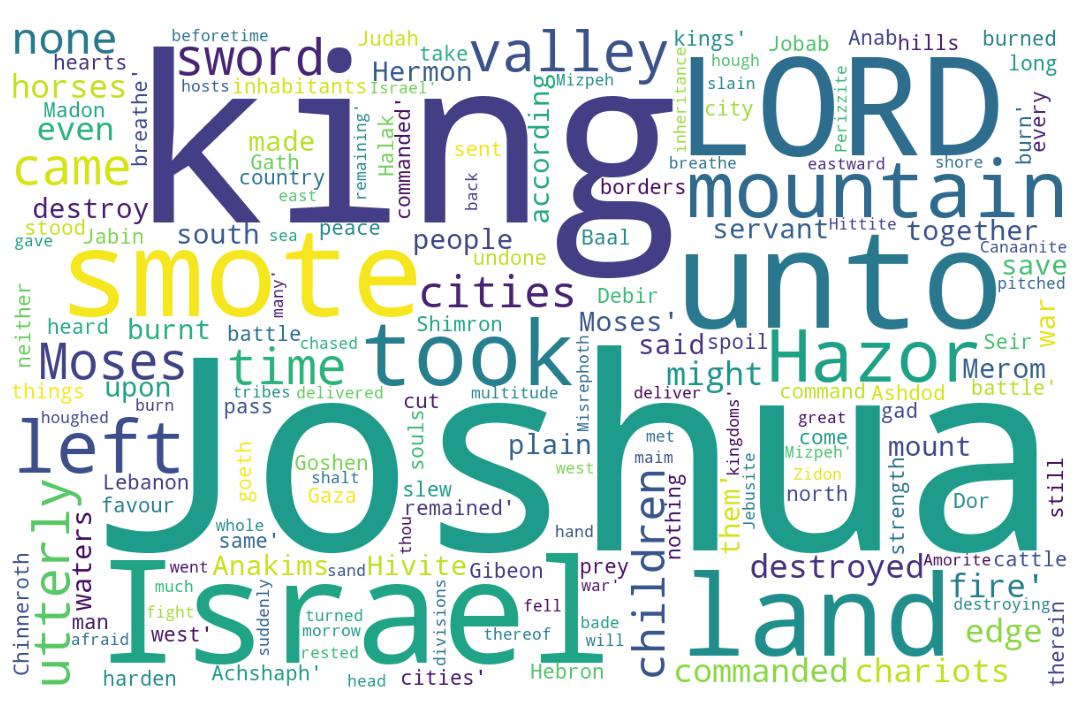
\includegraphics[width=\linewidth]{06OT-Joshua/Joshua11-WordCloud.jpg}
  \caption{Joshua 11 Word Cloud}
  \label{fig:Joshua 11 Word Cloud}
\end{figure}

\marginpar{\scriptsize \centering \fcolorbox{bone}{lime}{\textbf{THE SOUTHERN CAMPAIGN}}\\ (Joshua 11) \begin{compactenum}[I.][8]
	\item \textbf{Responisbility to Fight} \index[scripture]{Joshua!Jsh 11:01}  (Jsh 11:1) 
	\item The Enemy's \textbf{Resources} \index[scripture]{Joshua!Jsh 11:04}  (Jsh 11:4)
	\item The Enemy's \textbf{Resistance} \index[scripture]{Joshua!Jsh 11:05}  (Jsh 11:5)
	\item The \textbf{Readiness} to Fight the Long Battles \index[scripture]{Joshua!Jsh 11:18}  (Jsh 11:18)
	\item The \textbf{Reknowned} Giants \index[scripture]{Joshua!Jsh 11:21}  (Jsh 11:21)
	\item  Where the Enemy \textbf{Remained}  \index[scripture]{Joshua!Jsh 11:22}  (Jsh 11:22)
	\item  \textbf{Rest} in the Land \index[scripture]{Joshua!Jsh 11:23}  (Jsh 11:23)
\end{compactenum}}




\footnote{\textcolor[rgb]{0.00,0.25,0.00}{\hyperlink{TOC}{Return to end of Table of Contents.}}}\footnote{\href{https://audiobible.com/bible/joshua_11.html}{\textcolor[cmyk]{0.99998,1,0,0}{Joshua 11 Audio}}}\textcolor[cmyk]{0.99998,1,0,0}{\fcolorbox{bone}{bone}{And} it came \fcolorbox{bone}{bone}{to} pass, when Jabin king of Hazor had heard \emph{those} \emph{things}, that he sent \fcolorbox{bone}{bone}{to} Jobab king of Madon, and \fcolorbox{bone}{bone}{to} the king of Shimron, and \fcolorbox{bone}{bone}{to} the king of Achshaph,}
[2] \textcolor[cmyk]{0.99998,1,0,0}{\fcolorbox{bone}{bone}{And} \fcolorbox{bone}{bone}{to} the kings that \emph{were} on the north of the mountains, and of the plains south of Chinneroth, and \fcolorbox{bone}{bone}{in} the valley, and \fcolorbox{bone}{bone}{in} the borders of Dor on the west,}
[3] \textcolor[cmyk]{0.99998,1,0,0}{\emph{And} \emph{to} the Canaanite on the east and on the west, and \emph{to} the Amorite, and the Hittite, and the Perizzite, and the Jebusite \fcolorbox{bone}{bone}{in} the mountains, and \emph{to} the Hivite under Hermon \fcolorbox{bone}{bone}{in} the land of Mizpeh.}
[4] \textcolor[cmyk]{0.99998,1,0,0}{\fcolorbox{bone}{bone}{And} \fcolorbox{bone}{bone}{they} went out, \fcolorbox{bone}{bone}{they} and all their hosts \fcolorbox{bone}{bone}{with} them, much people, even as the sand that \emph{is} upon the sea shore \fcolorbox{bone}{bone}{in} multitude, \fcolorbox{bone}{bone}{with} horses and chariots very many.}
[5] \textcolor[cmyk]{0.99998,1,0,0}{\fcolorbox{bone}{bone}{And} when all these kings were met together, \fcolorbox{bone}{bone}{they} came and pitched together at the waters of Merom, \fcolorbox{bone}{bone}{to} fight against Israel.}\\
\\
\P \textcolor[cmyk]{0.99998,1,0,0}{\fcolorbox{bone}{bone}{And} the LORD said unto Joshua, Be not afraid because of them: for \fcolorbox{bone}{bone}{to} morrow about this time will I deliver them up all slain before Israel: thou shalt hough their horses, and burn their chariots \fcolorbox{bone}{bone}{with} fire.}
[7] \textcolor[cmyk]{0.99998,1,0,0}{So Joshua came, and all the people of war \fcolorbox{bone}{bone}{with} him, against them by the waters of Merom suddenly; and \fcolorbox{bone}{bone}{they} fell upon them.}
[8] \textcolor[cmyk]{0.99998,1,0,0}{\fcolorbox{bone}{bone}{And} the LORD delivered them into the hand of Israel, who smote them, and chased them unto great Zidon, and unto Misrephoth-maim, and unto the valley of Mizpeh eastward; and \fcolorbox{bone}{bone}{they} smote them, until \fcolorbox{bone}{bone}{they} left them none remaining.}
[9] \textcolor[cmyk]{0.99998,1,0,0}{\fcolorbox{bone}{bone}{And} Joshua did unto them as the LORD bade him: he houghed their horses, and burnt their chariots \fcolorbox{bone}{bone}{with} fire.}\\
\\
\P \textcolor[cmyk]{0.99998,1,0,0}{\fcolorbox{bone}{bone}{And} Joshua at that time turned back, and took Hazor, and smote the king thereof \fcolorbox{bone}{bone}{with} the sword: for Hazor beforetime was the head of all those kingdoms.}
[11] \textcolor[cmyk]{0.99998,1,0,0}{\fcolorbox{bone}{bone}{And} \fcolorbox{bone}{bone}{they} smote all the souls that \emph{were} therein \fcolorbox{bone}{bone}{with} the edge of the sword, utterly destroying \emph{them}: there was not any left \fcolorbox{bone}{bone}{to} breathe: and he burnt Hazor \fcolorbox{bone}{bone}{with} fire.}
[12] \textcolor[cmyk]{0.99998,1,0,0}{\fcolorbox{bone}{bone}{And} all the cities of those kings, and all the kings of them, did Joshua take, and smote them \fcolorbox{bone}{bone}{with} the edge of the sword, \emph{and} he utterly destroyed them, as Moses the servant of the LORD commanded.}
[13] \textcolor[cmyk]{0.99998,1,0,0}{But \emph{as} \emph{for} the cities that stood still \fcolorbox{bone}{bone}{in} their strength, Israel burned none of them, save Hazor only; \emph{that} did Joshua burn.}
[14] \textcolor[cmyk]{0.99998,1,0,0}{\fcolorbox{bone}{bone}{And} all the spoil of these cities, and the cattle, the children of Israel took for a prey unto themselves; but every man \fcolorbox{bone}{bone}{they} smote \fcolorbox{bone}{bone}{with} the edge of the sword, until \fcolorbox{bone}{bone}{they} had destroyed them, neither left \fcolorbox{bone}{bone}{they} any \fcolorbox{bone}{bone}{to} breathe.}\\
\\
\P \textcolor[cmyk]{0.99998,1,0,0}{As the LORD commanded Moses his servant, so did Moses command Joshua, and so did Joshua; he left nothing undone of all that the LORD commanded Moses.}
[16] \textcolor[cmyk]{0.99998,1,0,0}{So Joshua took all that land, the hills, and all the south country, and all the land of Goshen, and the valley, and the plain, and the mountain of Israel, and the valley of the same;}
[17] \textcolor[cmyk]{0.99998,1,0,0}{\emph{Even} from the mount Halak, that goeth up \fcolorbox{bone}{bone}{to} Seir, even unto Baal-gad \fcolorbox{bone}{bone}{in} the valley of Lebanon under mount Hermon: and all their kings he took, and smote them, and slew them.}
[18] \textcolor[cmyk]{0.99998,1,0,0}{Joshua made war a long time \fcolorbox{bone}{bone}{with} all those kings.}
[19] \textcolor[cmyk]{0.99998,1,0,0}{There was not a city that made peace \fcolorbox{bone}{bone}{with} the children of Israel, save the Hivites the inhabitants of Gibeon: all \emph{other} \fcolorbox{bone}{bone}{they} took \fcolorbox{bone}{bone}{in} battle.}
[20] \textcolor[cmyk]{0.99998,1,0,0}{For it was of the LORD \fcolorbox{bone}{bone}{to} harden their hearts, that \fcolorbox{bone}{bone}{they} should come against Israel \fcolorbox{bone}{bone}{in} battle, that he might destroy them utterly, \emph{and} that \fcolorbox{bone}{bone}{they} might have no favour, but that he might destroy them, as the LORD commanded Moses.}\\
\\
\P \textcolor[cmyk]{0.99998,1,0,0}{\fcolorbox{bone}{bone}{And} at that time came Joshua, and cut off the Anakims from the mountains, from Hebron, from Debir, from Anab, and from all the mountains of Judah, and from all the mountains of Israel: Joshua destroyed them utterly \fcolorbox{bone}{bone}{with} their cities.}
[22] \textcolor[cmyk]{0.99998,1,0,0}{There was none of the Anakims left \fcolorbox{bone}{bone}{in} the land of the children of Israel: only \fcolorbox{bone}{bone}{in} Gaza, \fcolorbox{bone}{bone}{in} Gath, and \fcolorbox{bone}{bone}{in} Ashdod, there remained.}
[23] \textcolor[cmyk]{0.99998,1,0,0}{So Joshua took the whole land, according \fcolorbox{bone}{bone}{to} all that the LORD said unto Moses; and Joshua gave it for an inheritance unto Israel according \fcolorbox{bone}{bone}{to} their divisions by their tribes. \fcolorbox{bone}{bone}{And} the land rested from war.}
\index[NWIV]{34!Joshua!Jos 11:1}\index[AWIP]{And!Joshua!Jos 11:1}\index[AWIP]{it!Joshua!Jos 11:1}\index[AWIP]{came!Joshua!Jos 11:1}\index[AWIP]{to!Joshua!Jos 11:1}\index[AWIP]{to!Joshua!Jos 11:1 (2)}\index[AWIP]{to!Joshua!Jos 11:1 (3)}\index[AWIP]{to!Joshua!Jos 11:1 (4)}\index[AWIP]{pass!Joshua!Jos 11:1}\index[AWIP]{when!Joshua!Jos 11:1}\index[AWIP]{Jabin!Joshua!Jos 11:1}\index[AWIP]{king!Joshua!Jos 11:1}\index[AWIP]{king!Joshua!Jos 11:1 (2)}\index[AWIP]{king!Joshua!Jos 11:1 (3)}\index[AWIP]{king!Joshua!Jos 11:1 (4)}\index[AWIP]{of!Joshua!Jos 11:1}\index[AWIP]{of!Joshua!Jos 11:1 (2)}\index[AWIP]{of!Joshua!Jos 11:1 (3)}\index[AWIP]{of!Joshua!Jos 11:1 (4)}\index[AWIP]{Hazor!Joshua!Jos 11:1}\index[AWIP]{had!Joshua!Jos 11:1}\index[AWIP]{heard!Joshua!Jos 11:1}\index[AWIP]{\emph{those}!Joshua!Jos 11:1}\index[AWIP]{\emph{things}!Joshua!Jos 11:1}\index[AWIP]{that!Joshua!Jos 11:1}\index[AWIP]{he!Joshua!Jos 11:1}\index[AWIP]{sent!Joshua!Jos 11:1}\index[AWIP]{Jobab!Joshua!Jos 11:1}\index[AWIP]{Madon!Joshua!Jos 11:1}\index[AWIP]{and!Joshua!Jos 11:1}\index[AWIP]{and!Joshua!Jos 11:1 (2)}\index[AWIP]{the!Joshua!Jos 11:1}\index[AWIP]{the!Joshua!Jos 11:1 (2)}\index[AWIP]{Shimron!Joshua!Jos 11:1}\index[AWIP]{Achshaph!Joshua!Jos 11:1}\index[AWIP]{\emph{those}!Joshua!Jos 11:1}\index[AWIP]{\emph{things}!Joshua!Jos 11:1}

\index[NWIV]{32!Joshua!Jos 11:2}\index[AWIP]{And!Joshua!Jos 11:2}\index[AWIP]{to!Joshua!Jos 11:2}\index[AWIP]{the!Joshua!Jos 11:2}\index[AWIP]{the!Joshua!Jos 11:2 (2)}\index[AWIP]{the!Joshua!Jos 11:2 (3)}\index[AWIP]{the!Joshua!Jos 11:2 (4)}\index[AWIP]{the!Joshua!Jos 11:2 (5)}\index[AWIP]{the!Joshua!Jos 11:2 (6)}\index[AWIP]{the!Joshua!Jos 11:2 (7)}\index[AWIP]{kings!Joshua!Jos 11:2}\index[AWIP]{that!Joshua!Jos 11:2}\index[AWIP]{\emph{were}!Joshua!Jos 11:2}\index[AWIP]{on!Joshua!Jos 11:2}\index[AWIP]{on!Joshua!Jos 11:2 (2)}\index[AWIP]{north!Joshua!Jos 11:2}\index[AWIP]{of!Joshua!Jos 11:2}\index[AWIP]{of!Joshua!Jos 11:2 (2)}\index[AWIP]{of!Joshua!Jos 11:2 (3)}\index[AWIP]{of!Joshua!Jos 11:2 (4)}\index[AWIP]{mountains!Joshua!Jos 11:2}\index[AWIP]{and!Joshua!Jos 11:2}\index[AWIP]{and!Joshua!Jos 11:2 (2)}\index[AWIP]{and!Joshua!Jos 11:2 (3)}\index[AWIP]{plains!Joshua!Jos 11:2}\index[AWIP]{south!Joshua!Jos 11:2}\index[AWIP]{Chinneroth!Joshua!Jos 11:2}\index[AWIP]{in!Joshua!Jos 11:2}\index[AWIP]{in!Joshua!Jos 11:2 (2)}\index[AWIP]{valley!Joshua!Jos 11:2}\index[AWIP]{borders!Joshua!Jos 11:2}\index[AWIP]{Dor!Joshua!Jos 11:2}\index[AWIP]{west!Joshua!Jos 11:2}\index[AWIP]{\emph{were}!Joshua!Jos 11:2}

\index[NWIV]{38!Joshua!Jos 11:3}\index[AWIP]{\emph{And}!Joshua!Jos 11:3}\index[AWIP]{\emph{to}!Joshua!Jos 11:3}\index[AWIP]{\emph{to}!Joshua!Jos 11:3 (2)}\index[AWIP]{\emph{to}!Joshua!Jos 11:3 (3)}\index[AWIP]{the!Joshua!Jos 11:3}\index[AWIP]{the!Joshua!Jos 11:3 (2)}\index[AWIP]{the!Joshua!Jos 11:3 (3)}\index[AWIP]{the!Joshua!Jos 11:3 (4)}\index[AWIP]{the!Joshua!Jos 11:3 (5)}\index[AWIP]{the!Joshua!Jos 11:3 (6)}\index[AWIP]{the!Joshua!Jos 11:3 (7)}\index[AWIP]{the!Joshua!Jos 11:3 (8)}\index[AWIP]{the!Joshua!Jos 11:3 (9)}\index[AWIP]{the!Joshua!Jos 11:3 (10)}\index[AWIP]{Canaanite!Joshua!Jos 11:3}\index[AWIP]{on!Joshua!Jos 11:3}\index[AWIP]{on!Joshua!Jos 11:3 (2)}\index[AWIP]{east!Joshua!Jos 11:3}\index[AWIP]{and!Joshua!Jos 11:3}\index[AWIP]{and!Joshua!Jos 11:3 (2)}\index[AWIP]{and!Joshua!Jos 11:3 (3)}\index[AWIP]{and!Joshua!Jos 11:3 (4)}\index[AWIP]{and!Joshua!Jos 11:3 (5)}\index[AWIP]{and!Joshua!Jos 11:3 (6)}\index[AWIP]{west!Joshua!Jos 11:3}\index[AWIP]{Amorite!Joshua!Jos 11:3}\index[AWIP]{Hittite!Joshua!Jos 11:3}\index[AWIP]{Perizzite!Joshua!Jos 11:3}\index[AWIP]{Jebusite!Joshua!Jos 11:3}\index[AWIP]{in!Joshua!Jos 11:3}\index[AWIP]{in!Joshua!Jos 11:3 (2)}\index[AWIP]{mountains!Joshua!Jos 11:3}\index[AWIP]{Hivite!Joshua!Jos 11:3}\index[AWIP]{under!Joshua!Jos 11:3}\index[AWIP]{Hermon!Joshua!Jos 11:3}\index[AWIP]{land!Joshua!Jos 11:3}\index[AWIP]{of!Joshua!Jos 11:3}\index[AWIP]{Mizpeh!Joshua!Jos 11:3}\index[AWIP]{\emph{And}!Joshua!Jos 11:3}\index[AWIP]{\emph{to}!Joshua!Jos 11:3}\index[AWIP]{\emph{to}!Joshua!Jos 11:3 (2)}\index[AWIP]{\emph{to}!Joshua!Jos 11:3 (3)}

\index[NWIV]{31!Joshua!Jos 11:4}\index[AWIP]{And!Joshua!Jos 11:4}\index[AWIP]{they!Joshua!Jos 11:4}\index[AWIP]{they!Joshua!Jos 11:4 (2)}\index[AWIP]{went!Joshua!Jos 11:4}\index[AWIP]{out!Joshua!Jos 11:4}\index[AWIP]{and!Joshua!Jos 11:4}\index[AWIP]{and!Joshua!Jos 11:4 (2)}\index[AWIP]{all!Joshua!Jos 11:4}\index[AWIP]{their!Joshua!Jos 11:4}\index[AWIP]{hosts!Joshua!Jos 11:4}\index[AWIP]{with!Joshua!Jos 11:4}\index[AWIP]{with!Joshua!Jos 11:4 (2)}\index[AWIP]{them!Joshua!Jos 11:4}\index[AWIP]{much!Joshua!Jos 11:4}\index[AWIP]{people!Joshua!Jos 11:4}\index[AWIP]{even!Joshua!Jos 11:4}\index[AWIP]{as!Joshua!Jos 11:4}\index[AWIP]{the!Joshua!Jos 11:4}\index[AWIP]{the!Joshua!Jos 11:4 (2)}\index[AWIP]{sand!Joshua!Jos 11:4}\index[AWIP]{that!Joshua!Jos 11:4}\index[AWIP]{\emph{is}!Joshua!Jos 11:4}\index[AWIP]{upon!Joshua!Jos 11:4}\index[AWIP]{sea!Joshua!Jos 11:4}\index[AWIP]{shore!Joshua!Jos 11:4}\index[AWIP]{in!Joshua!Jos 11:4}\index[AWIP]{multitude!Joshua!Jos 11:4}\index[AWIP]{horses!Joshua!Jos 11:4}\index[AWIP]{chariots!Joshua!Jos 11:4}\index[AWIP]{very!Joshua!Jos 11:4}\index[AWIP]{many!Joshua!Jos 11:4}\index[AWIP]{\emph{is}!Joshua!Jos 11:4}

\index[NWIV]{22!Joshua!Jos 11:5}\index[AWIP]{And!Joshua!Jos 11:5}\index[AWIP]{when!Joshua!Jos 11:5}\index[AWIP]{all!Joshua!Jos 11:5}\index[AWIP]{these!Joshua!Jos 11:5}\index[AWIP]{kings!Joshua!Jos 11:5}\index[AWIP]{were!Joshua!Jos 11:5}\index[AWIP]{met!Joshua!Jos 11:5}\index[AWIP]{together!Joshua!Jos 11:5}\index[AWIP]{together!Joshua!Jos 11:5 (2)}\index[AWIP]{they!Joshua!Jos 11:5}\index[AWIP]{came!Joshua!Jos 11:5}\index[AWIP]{and!Joshua!Jos 11:5}\index[AWIP]{pitched!Joshua!Jos 11:5}\index[AWIP]{at!Joshua!Jos 11:5}\index[AWIP]{the!Joshua!Jos 11:5}\index[AWIP]{waters!Joshua!Jos 11:5}\index[AWIP]{of!Joshua!Jos 11:5}\index[AWIP]{Merom!Joshua!Jos 11:5}\index[AWIP]{to!Joshua!Jos 11:5}\index[AWIP]{fight!Joshua!Jos 11:5}\index[AWIP]{against!Joshua!Jos 11:5}\index[AWIP]{Israel!Joshua!Jos 11:5}

\index[NWIV]{38!Joshua!Jos 11:6}\index[AWIP]{And!Joshua!Jos 11:6}\index[AWIP]{the!Joshua!Jos 11:6}\index[AWIP]{LORD!Joshua!Jos 11:6}\index[AWIP]{said!Joshua!Jos 11:6}\index[AWIP]{unto!Joshua!Jos 11:6}\index[AWIP]{Joshua!Joshua!Jos 11:6}\index[AWIP]{Be!Joshua!Jos 11:6}\index[AWIP]{not!Joshua!Jos 11:6}\index[AWIP]{afraid!Joshua!Jos 11:6}\index[AWIP]{because!Joshua!Jos 11:6}\index[AWIP]{of!Joshua!Jos 11:6}\index[AWIP]{them!Joshua!Jos 11:6}\index[AWIP]{them!Joshua!Jos 11:6 (2)}\index[AWIP]{for!Joshua!Jos 11:6}\index[AWIP]{to!Joshua!Jos 11:6}\index[AWIP]{morrow!Joshua!Jos 11:6}\index[AWIP]{about!Joshua!Jos 11:6}\index[AWIP]{this!Joshua!Jos 11:6}\index[AWIP]{time!Joshua!Jos 11:6}\index[AWIP]{will!Joshua!Jos 11:6}\index[AWIP]{I!Joshua!Jos 11:6}\index[AWIP]{deliver!Joshua!Jos 11:6}\index[AWIP]{up!Joshua!Jos 11:6}\index[AWIP]{all!Joshua!Jos 11:6}\index[AWIP]{slain!Joshua!Jos 11:6}\index[AWIP]{before!Joshua!Jos 11:6}\index[AWIP]{Israel!Joshua!Jos 11:6}\index[AWIP]{thou!Joshua!Jos 11:6}\index[AWIP]{shalt!Joshua!Jos 11:6}\index[AWIP]{hough!Joshua!Jos 11:6}\index[AWIP]{their!Joshua!Jos 11:6}\index[AWIP]{their!Joshua!Jos 11:6 (2)}\index[AWIP]{horses!Joshua!Jos 11:6}\index[AWIP]{and!Joshua!Jos 11:6}\index[AWIP]{burn!Joshua!Jos 11:6}\index[AWIP]{chariots!Joshua!Jos 11:6}\index[AWIP]{with!Joshua!Jos 11:6}\index[AWIP]{fire!Joshua!Jos 11:6}

\index[NWIV]{24!Joshua!Jos 11:7}\index[AWIP]{So!Joshua!Jos 11:7}\index[AWIP]{Joshua!Joshua!Jos 11:7}\index[AWIP]{came!Joshua!Jos 11:7}\index[AWIP]{and!Joshua!Jos 11:7}\index[AWIP]{and!Joshua!Jos 11:7 (2)}\index[AWIP]{all!Joshua!Jos 11:7}\index[AWIP]{the!Joshua!Jos 11:7}\index[AWIP]{the!Joshua!Jos 11:7 (2)}\index[AWIP]{people!Joshua!Jos 11:7}\index[AWIP]{of!Joshua!Jos 11:7}\index[AWIP]{of!Joshua!Jos 11:7 (2)}\index[AWIP]{war!Joshua!Jos 11:7}\index[AWIP]{with!Joshua!Jos 11:7}\index[AWIP]{him!Joshua!Jos 11:7}\index[AWIP]{against!Joshua!Jos 11:7}\index[AWIP]{them!Joshua!Jos 11:7}\index[AWIP]{them!Joshua!Jos 11:7 (2)}\index[AWIP]{by!Joshua!Jos 11:7}\index[AWIP]{waters!Joshua!Jos 11:7}\index[AWIP]{Merom!Joshua!Jos 11:7}\index[AWIP]{suddenly!Joshua!Jos 11:7}\index[AWIP]{they!Joshua!Jos 11:7}\index[AWIP]{fell!Joshua!Jos 11:7}\index[AWIP]{upon!Joshua!Jos 11:7}

\index[NWIV]{39!Joshua!Jos 11:8}\index[AWIP]{And!Joshua!Jos 11:8}\index[AWIP]{the!Joshua!Jos 11:8}\index[AWIP]{the!Joshua!Jos 11:8 (2)}\index[AWIP]{the!Joshua!Jos 11:8 (3)}\index[AWIP]{LORD!Joshua!Jos 11:8}\index[AWIP]{delivered!Joshua!Jos 11:8}\index[AWIP]{them!Joshua!Jos 11:8}\index[AWIP]{them!Joshua!Jos 11:8 (2)}\index[AWIP]{them!Joshua!Jos 11:8 (3)}\index[AWIP]{them!Joshua!Jos 11:8 (4)}\index[AWIP]{them!Joshua!Jos 11:8 (5)}\index[AWIP]{into!Joshua!Jos 11:8}\index[AWIP]{hand!Joshua!Jos 11:8}\index[AWIP]{of!Joshua!Jos 11:8}\index[AWIP]{of!Joshua!Jos 11:8 (2)}\index[AWIP]{Israel!Joshua!Jos 11:8}\index[AWIP]{who!Joshua!Jos 11:8}\index[AWIP]{smote!Joshua!Jos 11:8}\index[AWIP]{smote!Joshua!Jos 11:8 (2)}\index[AWIP]{and!Joshua!Jos 11:8}\index[AWIP]{and!Joshua!Jos 11:8 (2)}\index[AWIP]{and!Joshua!Jos 11:8 (3)}\index[AWIP]{and!Joshua!Jos 11:8 (4)}\index[AWIP]{chased!Joshua!Jos 11:8}\index[AWIP]{unto!Joshua!Jos 11:8}\index[AWIP]{unto!Joshua!Jos 11:8 (2)}\index[AWIP]{unto!Joshua!Jos 11:8 (3)}\index[AWIP]{great!Joshua!Jos 11:8}\index[AWIP]{Zidon!Joshua!Jos 11:8}\index[AWIP]{Misrephoth-maim!Joshua!Jos 11:8}\index[AWIP]{valley!Joshua!Jos 11:8}\index[AWIP]{Mizpeh!Joshua!Jos 11:8}\index[AWIP]{eastward!Joshua!Jos 11:8}\index[AWIP]{they!Joshua!Jos 11:8}\index[AWIP]{they!Joshua!Jos 11:8 (2)}\index[AWIP]{until!Joshua!Jos 11:8}\index[AWIP]{left!Joshua!Jos 11:8}\index[AWIP]{none!Joshua!Jos 11:8}\index[AWIP]{remaining!Joshua!Jos 11:8}

\index[NWIV]{20!Joshua!Jos 11:9}\index[AWIP]{And!Joshua!Jos 11:9}\index[AWIP]{Joshua!Joshua!Jos 11:9}\index[AWIP]{did!Joshua!Jos 11:9}\index[AWIP]{unto!Joshua!Jos 11:9}\index[AWIP]{them!Joshua!Jos 11:9}\index[AWIP]{as!Joshua!Jos 11:9}\index[AWIP]{the!Joshua!Jos 11:9}\index[AWIP]{LORD!Joshua!Jos 11:9}\index[AWIP]{bade!Joshua!Jos 11:9}\index[AWIP]{him!Joshua!Jos 11:9}\index[AWIP]{he!Joshua!Jos 11:9}\index[AWIP]{houghed!Joshua!Jos 11:9}\index[AWIP]{their!Joshua!Jos 11:9}\index[AWIP]{their!Joshua!Jos 11:9 (2)}\index[AWIP]{horses!Joshua!Jos 11:9}\index[AWIP]{and!Joshua!Jos 11:9}\index[AWIP]{burnt!Joshua!Jos 11:9}\index[AWIP]{chariots!Joshua!Jos 11:9}\index[AWIP]{with!Joshua!Jos 11:9}\index[AWIP]{fire!Joshua!Jos 11:9}

\index[NWIV]{28!Joshua!Jos 11:10}\index[AWIP]{And!Joshua!Jos 11:10}\index[AWIP]{Joshua!Joshua!Jos 11:10}\index[AWIP]{at!Joshua!Jos 11:10}\index[AWIP]{that!Joshua!Jos 11:10}\index[AWIP]{time!Joshua!Jos 11:10}\index[AWIP]{turned!Joshua!Jos 11:10}\index[AWIP]{back!Joshua!Jos 11:10}\index[AWIP]{and!Joshua!Jos 11:10}\index[AWIP]{and!Joshua!Jos 11:10 (2)}\index[AWIP]{took!Joshua!Jos 11:10}\index[AWIP]{Hazor!Joshua!Jos 11:10}\index[AWIP]{Hazor!Joshua!Jos 11:10 (2)}\index[AWIP]{smote!Joshua!Jos 11:10}\index[AWIP]{the!Joshua!Jos 11:10}\index[AWIP]{the!Joshua!Jos 11:10 (2)}\index[AWIP]{the!Joshua!Jos 11:10 (3)}\index[AWIP]{king!Joshua!Jos 11:10}\index[AWIP]{thereof!Joshua!Jos 11:10}\index[AWIP]{with!Joshua!Jos 11:10}\index[AWIP]{sword!Joshua!Jos 11:10}\index[AWIP]{for!Joshua!Jos 11:10}\index[AWIP]{beforetime!Joshua!Jos 11:10}\index[AWIP]{was!Joshua!Jos 11:10}\index[AWIP]{head!Joshua!Jos 11:10}\index[AWIP]{of!Joshua!Jos 11:10}\index[AWIP]{all!Joshua!Jos 11:10}\index[AWIP]{those!Joshua!Jos 11:10}\index[AWIP]{kingdoms!Joshua!Jos 11:10}

\index[NWIV]{31!Joshua!Jos 11:11}\index[AWIP]{And!Joshua!Jos 11:11}\index[AWIP]{they!Joshua!Jos 11:11}\index[AWIP]{smote!Joshua!Jos 11:11}\index[AWIP]{all!Joshua!Jos 11:11}\index[AWIP]{the!Joshua!Jos 11:11}\index[AWIP]{the!Joshua!Jos 11:11 (2)}\index[AWIP]{the!Joshua!Jos 11:11 (3)}\index[AWIP]{souls!Joshua!Jos 11:11}\index[AWIP]{that!Joshua!Jos 11:11}\index[AWIP]{\emph{were}!Joshua!Jos 11:11}\index[AWIP]{therein!Joshua!Jos 11:11}\index[AWIP]{with!Joshua!Jos 11:11}\index[AWIP]{with!Joshua!Jos 11:11 (2)}\index[AWIP]{edge!Joshua!Jos 11:11}\index[AWIP]{of!Joshua!Jos 11:11}\index[AWIP]{sword!Joshua!Jos 11:11}\index[AWIP]{utterly!Joshua!Jos 11:11}\index[AWIP]{destroying!Joshua!Jos 11:11}\index[AWIP]{\emph{them}!Joshua!Jos 11:11}\index[AWIP]{there!Joshua!Jos 11:11}\index[AWIP]{was!Joshua!Jos 11:11}\index[AWIP]{not!Joshua!Jos 11:11}\index[AWIP]{any!Joshua!Jos 11:11}\index[AWIP]{left!Joshua!Jos 11:11}\index[AWIP]{to!Joshua!Jos 11:11}\index[AWIP]{breathe!Joshua!Jos 11:11}\index[AWIP]{and!Joshua!Jos 11:11}\index[AWIP]{he!Joshua!Jos 11:11}\index[AWIP]{burnt!Joshua!Jos 11:11}\index[AWIP]{Hazor!Joshua!Jos 11:11}\index[AWIP]{fire!Joshua!Jos 11:11}\index[AWIP]{\emph{were}!Joshua!Jos 11:11}\index[AWIP]{\emph{them}!Joshua!Jos 11:11}

\index[NWIV]{38!Joshua!Jos 11:12}\index[AWIP]{And!Joshua!Jos 11:12}\index[AWIP]{all!Joshua!Jos 11:12}\index[AWIP]{all!Joshua!Jos 11:12 (2)}\index[AWIP]{the!Joshua!Jos 11:12}\index[AWIP]{the!Joshua!Jos 11:12 (2)}\index[AWIP]{the!Joshua!Jos 11:12 (3)}\index[AWIP]{the!Joshua!Jos 11:12 (4)}\index[AWIP]{the!Joshua!Jos 11:12 (5)}\index[AWIP]{the!Joshua!Jos 11:12 (6)}\index[AWIP]{cities!Joshua!Jos 11:12}\index[AWIP]{of!Joshua!Jos 11:12}\index[AWIP]{of!Joshua!Jos 11:12 (2)}\index[AWIP]{of!Joshua!Jos 11:12 (3)}\index[AWIP]{of!Joshua!Jos 11:12 (4)}\index[AWIP]{those!Joshua!Jos 11:12}\index[AWIP]{kings!Joshua!Jos 11:12}\index[AWIP]{kings!Joshua!Jos 11:12 (2)}\index[AWIP]{and!Joshua!Jos 11:12}\index[AWIP]{and!Joshua!Jos 11:12 (2)}\index[AWIP]{them!Joshua!Jos 11:12}\index[AWIP]{them!Joshua!Jos 11:12 (2)}\index[AWIP]{them!Joshua!Jos 11:12 (3)}\index[AWIP]{did!Joshua!Jos 11:12}\index[AWIP]{Joshua!Joshua!Jos 11:12}\index[AWIP]{take!Joshua!Jos 11:12}\index[AWIP]{smote!Joshua!Jos 11:12}\index[AWIP]{with!Joshua!Jos 11:12}\index[AWIP]{edge!Joshua!Jos 11:12}\index[AWIP]{sword!Joshua!Jos 11:12}\index[AWIP]{\emph{and}!Joshua!Jos 11:12}\index[AWIP]{he!Joshua!Jos 11:12}\index[AWIP]{utterly!Joshua!Jos 11:12}\index[AWIP]{destroyed!Joshua!Jos 11:12}\index[AWIP]{as!Joshua!Jos 11:12}\index[AWIP]{Moses!Joshua!Jos 11:12}\index[AWIP]{servant!Joshua!Jos 11:12}\index[AWIP]{LORD!Joshua!Jos 11:12}\index[AWIP]{commanded!Joshua!Jos 11:12}\index[AWIP]{\emph{and}!Joshua!Jos 11:12}

\index[NWIV]{23!Joshua!Jos 11:13}\index[AWIP]{But!Joshua!Jos 11:13}\index[AWIP]{\emph{as}!Joshua!Jos 11:13}\index[AWIP]{\emph{for}!Joshua!Jos 11:13}\index[AWIP]{the!Joshua!Jos 11:13}\index[AWIP]{cities!Joshua!Jos 11:13}\index[AWIP]{that!Joshua!Jos 11:13}\index[AWIP]{stood!Joshua!Jos 11:13}\index[AWIP]{still!Joshua!Jos 11:13}\index[AWIP]{in!Joshua!Jos 11:13}\index[AWIP]{their!Joshua!Jos 11:13}\index[AWIP]{strength!Joshua!Jos 11:13}\index[AWIP]{Israel!Joshua!Jos 11:13}\index[AWIP]{burned!Joshua!Jos 11:13}\index[AWIP]{none!Joshua!Jos 11:13}\index[AWIP]{of!Joshua!Jos 11:13}\index[AWIP]{them!Joshua!Jos 11:13}\index[AWIP]{save!Joshua!Jos 11:13}\index[AWIP]{Hazor!Joshua!Jos 11:13}\index[AWIP]{only!Joshua!Jos 11:13}\index[AWIP]{\emph{that}!Joshua!Jos 11:13}\index[AWIP]{did!Joshua!Jos 11:13}\index[AWIP]{Joshua!Joshua!Jos 11:13}\index[AWIP]{burn!Joshua!Jos 11:13}\index[AWIP]{\emph{as}!Joshua!Jos 11:13}\index[AWIP]{\emph{for}!Joshua!Jos 11:13}\index[AWIP]{\emph{that}!Joshua!Jos 11:13}

\index[NWIV]{42!Joshua!Jos 11:14}\index[AWIP]{And!Joshua!Jos 11:14}\index[AWIP]{all!Joshua!Jos 11:14}\index[AWIP]{the!Joshua!Jos 11:14}\index[AWIP]{the!Joshua!Jos 11:14 (2)}\index[AWIP]{the!Joshua!Jos 11:14 (3)}\index[AWIP]{the!Joshua!Jos 11:14 (4)}\index[AWIP]{the!Joshua!Jos 11:14 (5)}\index[AWIP]{spoil!Joshua!Jos 11:14}\index[AWIP]{of!Joshua!Jos 11:14}\index[AWIP]{of!Joshua!Jos 11:14 (2)}\index[AWIP]{of!Joshua!Jos 11:14 (3)}\index[AWIP]{these!Joshua!Jos 11:14}\index[AWIP]{cities!Joshua!Jos 11:14}\index[AWIP]{and!Joshua!Jos 11:14}\index[AWIP]{cattle!Joshua!Jos 11:14}\index[AWIP]{children!Joshua!Jos 11:14}\index[AWIP]{Israel!Joshua!Jos 11:14}\index[AWIP]{took!Joshua!Jos 11:14}\index[AWIP]{for!Joshua!Jos 11:14}\index[AWIP]{a!Joshua!Jos 11:14}\index[AWIP]{prey!Joshua!Jos 11:14}\index[AWIP]{unto!Joshua!Jos 11:14}\index[AWIP]{themselves!Joshua!Jos 11:14}\index[AWIP]{but!Joshua!Jos 11:14}\index[AWIP]{every!Joshua!Jos 11:14}\index[AWIP]{man!Joshua!Jos 11:14}\index[AWIP]{they!Joshua!Jos 11:14}\index[AWIP]{they!Joshua!Jos 11:14 (2)}\index[AWIP]{they!Joshua!Jos 11:14 (3)}\index[AWIP]{smote!Joshua!Jos 11:14}\index[AWIP]{with!Joshua!Jos 11:14}\index[AWIP]{edge!Joshua!Jos 11:14}\index[AWIP]{sword!Joshua!Jos 11:14}\index[AWIP]{until!Joshua!Jos 11:14}\index[AWIP]{had!Joshua!Jos 11:14}\index[AWIP]{destroyed!Joshua!Jos 11:14}\index[AWIP]{them!Joshua!Jos 11:14}\index[AWIP]{neither!Joshua!Jos 11:14}\index[AWIP]{left!Joshua!Jos 11:14}\index[AWIP]{any!Joshua!Jos 11:14}\index[AWIP]{to!Joshua!Jos 11:14}\index[AWIP]{breathe!Joshua!Jos 11:14}

\index[NWIV]{27!Joshua!Jos 11:15}\index[AWIP]{As!Joshua!Jos 11:15}\index[AWIP]{the!Joshua!Jos 11:15}\index[AWIP]{the!Joshua!Jos 11:15 (2)}\index[AWIP]{LORD!Joshua!Jos 11:15}\index[AWIP]{LORD!Joshua!Jos 11:15 (2)}\index[AWIP]{commanded!Joshua!Jos 11:15}\index[AWIP]{commanded!Joshua!Jos 11:15 (2)}\index[AWIP]{Moses!Joshua!Jos 11:15}\index[AWIP]{Moses!Joshua!Jos 11:15 (2)}\index[AWIP]{Moses!Joshua!Jos 11:15 (3)}\index[AWIP]{his!Joshua!Jos 11:15}\index[AWIP]{servant!Joshua!Jos 11:15}\index[AWIP]{so!Joshua!Jos 11:15}\index[AWIP]{so!Joshua!Jos 11:15 (2)}\index[AWIP]{did!Joshua!Jos 11:15}\index[AWIP]{did!Joshua!Jos 11:15 (2)}\index[AWIP]{command!Joshua!Jos 11:15}\index[AWIP]{Joshua!Joshua!Jos 11:15}\index[AWIP]{Joshua!Joshua!Jos 11:15 (2)}\index[AWIP]{and!Joshua!Jos 11:15}\index[AWIP]{he!Joshua!Jos 11:15}\index[AWIP]{left!Joshua!Jos 11:15}\index[AWIP]{nothing!Joshua!Jos 11:15}\index[AWIP]{undone!Joshua!Jos 11:15}\index[AWIP]{of!Joshua!Jos 11:15}\index[AWIP]{all!Joshua!Jos 11:15}\index[AWIP]{that!Joshua!Jos 11:15}

\index[NWIV]{36!Joshua!Jos 11:16}\index[AWIP]{So!Joshua!Jos 11:16}\index[AWIP]{Joshua!Joshua!Jos 11:16}\index[AWIP]{took!Joshua!Jos 11:16}\index[AWIP]{all!Joshua!Jos 11:16}\index[AWIP]{all!Joshua!Jos 11:16 (2)}\index[AWIP]{all!Joshua!Jos 11:16 (3)}\index[AWIP]{that!Joshua!Jos 11:16}\index[AWIP]{land!Joshua!Jos 11:16}\index[AWIP]{land!Joshua!Jos 11:16 (2)}\index[AWIP]{the!Joshua!Jos 11:16}\index[AWIP]{the!Joshua!Jos 11:16 (2)}\index[AWIP]{the!Joshua!Jos 11:16 (3)}\index[AWIP]{the!Joshua!Jos 11:16 (4)}\index[AWIP]{the!Joshua!Jos 11:16 (5)}\index[AWIP]{the!Joshua!Jos 11:16 (6)}\index[AWIP]{the!Joshua!Jos 11:16 (7)}\index[AWIP]{the!Joshua!Jos 11:16 (8)}\index[AWIP]{hills!Joshua!Jos 11:16}\index[AWIP]{and!Joshua!Jos 11:16}\index[AWIP]{and!Joshua!Jos 11:16 (2)}\index[AWIP]{and!Joshua!Jos 11:16 (3)}\index[AWIP]{and!Joshua!Jos 11:16 (4)}\index[AWIP]{and!Joshua!Jos 11:16 (5)}\index[AWIP]{and!Joshua!Jos 11:16 (6)}\index[AWIP]{south!Joshua!Jos 11:16}\index[AWIP]{country!Joshua!Jos 11:16}\index[AWIP]{of!Joshua!Jos 11:16}\index[AWIP]{of!Joshua!Jos 11:16 (2)}\index[AWIP]{of!Joshua!Jos 11:16 (3)}\index[AWIP]{Goshen!Joshua!Jos 11:16}\index[AWIP]{valley!Joshua!Jos 11:16}\index[AWIP]{valley!Joshua!Jos 11:16 (2)}\index[AWIP]{plain!Joshua!Jos 11:16}\index[AWIP]{mountain!Joshua!Jos 11:16}\index[AWIP]{Israel!Joshua!Jos 11:16}\index[AWIP]{same!Joshua!Jos 11:16}

\index[NWIV]{33!Joshua!Jos 11:17}\index[AWIP]{\emph{Even}!Joshua!Jos 11:17}\index[AWIP]{from!Joshua!Jos 11:17}\index[AWIP]{the!Joshua!Jos 11:17}\index[AWIP]{the!Joshua!Jos 11:17 (2)}\index[AWIP]{mount!Joshua!Jos 11:17}\index[AWIP]{mount!Joshua!Jos 11:17 (2)}\index[AWIP]{Halak!Joshua!Jos 11:17}\index[AWIP]{that!Joshua!Jos 11:17}\index[AWIP]{goeth!Joshua!Jos 11:17}\index[AWIP]{up!Joshua!Jos 11:17}\index[AWIP]{to!Joshua!Jos 11:17}\index[AWIP]{Seir!Joshua!Jos 11:17}\index[AWIP]{even!Joshua!Jos 11:17}\index[AWIP]{unto!Joshua!Jos 11:17}\index[AWIP]{Baal-gad!Joshua!Jos 11:17}\index[AWIP]{in!Joshua!Jos 11:17}\index[AWIP]{valley!Joshua!Jos 11:17}\index[AWIP]{of!Joshua!Jos 11:17}\index[AWIP]{Lebanon!Joshua!Jos 11:17}\index[AWIP]{under!Joshua!Jos 11:17}\index[AWIP]{Hermon!Joshua!Jos 11:17}\index[AWIP]{and!Joshua!Jos 11:17}\index[AWIP]{and!Joshua!Jos 11:17 (2)}\index[AWIP]{and!Joshua!Jos 11:17 (3)}\index[AWIP]{all!Joshua!Jos 11:17}\index[AWIP]{their!Joshua!Jos 11:17}\index[AWIP]{kings!Joshua!Jos 11:17}\index[AWIP]{he!Joshua!Jos 11:17}\index[AWIP]{took!Joshua!Jos 11:17}\index[AWIP]{smote!Joshua!Jos 11:17}\index[AWIP]{them!Joshua!Jos 11:17}\index[AWIP]{them!Joshua!Jos 11:17 (2)}\index[AWIP]{slew!Joshua!Jos 11:17}\index[AWIP]{\emph{Even}!Joshua!Jos 11:17}

\index[NWIV]{10!Joshua!Jos 11:18}\index[AWIP]{Joshua!Joshua!Jos 11:18}\index[AWIP]{made!Joshua!Jos 11:18}\index[AWIP]{war!Joshua!Jos 11:18}\index[AWIP]{a!Joshua!Jos 11:18}\index[AWIP]{long!Joshua!Jos 11:18}\index[AWIP]{time!Joshua!Jos 11:18}\index[AWIP]{with!Joshua!Jos 11:18}\index[AWIP]{all!Joshua!Jos 11:18}\index[AWIP]{those!Joshua!Jos 11:18}\index[AWIP]{kings!Joshua!Jos 11:18}

\index[NWIV]{26!Joshua!Jos 11:19}\index[AWIP]{There!Joshua!Jos 11:19}\index[AWIP]{was!Joshua!Jos 11:19}\index[AWIP]{not!Joshua!Jos 11:19}\index[AWIP]{a!Joshua!Jos 11:19}\index[AWIP]{city!Joshua!Jos 11:19}\index[AWIP]{that!Joshua!Jos 11:19}\index[AWIP]{made!Joshua!Jos 11:19}\index[AWIP]{peace!Joshua!Jos 11:19}\index[AWIP]{with!Joshua!Jos 11:19}\index[AWIP]{the!Joshua!Jos 11:19}\index[AWIP]{the!Joshua!Jos 11:19 (2)}\index[AWIP]{the!Joshua!Jos 11:19 (3)}\index[AWIP]{children!Joshua!Jos 11:19}\index[AWIP]{of!Joshua!Jos 11:19}\index[AWIP]{of!Joshua!Jos 11:19 (2)}\index[AWIP]{Israel!Joshua!Jos 11:19}\index[AWIP]{save!Joshua!Jos 11:19}\index[AWIP]{Hivites!Joshua!Jos 11:19}\index[AWIP]{inhabitants!Joshua!Jos 11:19}\index[AWIP]{Gibeon!Joshua!Jos 11:19}\index[AWIP]{all!Joshua!Jos 11:19}\index[AWIP]{\emph{other}!Joshua!Jos 11:19}\index[AWIP]{they!Joshua!Jos 11:19}\index[AWIP]{took!Joshua!Jos 11:19}\index[AWIP]{in!Joshua!Jos 11:19}\index[AWIP]{battle!Joshua!Jos 11:19}\index[AWIP]{\emph{other}!Joshua!Jos 11:19}

\index[NWIV]{42!Joshua!Jos 11:20}\index[AWIP]{For!Joshua!Jos 11:20}\index[AWIP]{it!Joshua!Jos 11:20}\index[AWIP]{was!Joshua!Jos 11:20}\index[AWIP]{of!Joshua!Jos 11:20}\index[AWIP]{the!Joshua!Jos 11:20}\index[AWIP]{the!Joshua!Jos 11:20 (2)}\index[AWIP]{LORD!Joshua!Jos 11:20}\index[AWIP]{LORD!Joshua!Jos 11:20 (2)}\index[AWIP]{to!Joshua!Jos 11:20}\index[AWIP]{harden!Joshua!Jos 11:20}\index[AWIP]{their!Joshua!Jos 11:20}\index[AWIP]{hearts!Joshua!Jos 11:20}\index[AWIP]{that!Joshua!Jos 11:20}\index[AWIP]{that!Joshua!Jos 11:20 (2)}\index[AWIP]{that!Joshua!Jos 11:20 (3)}\index[AWIP]{that!Joshua!Jos 11:20 (4)}\index[AWIP]{they!Joshua!Jos 11:20}\index[AWIP]{they!Joshua!Jos 11:20 (2)}\index[AWIP]{should!Joshua!Jos 11:20}\index[AWIP]{come!Joshua!Jos 11:20}\index[AWIP]{against!Joshua!Jos 11:20}\index[AWIP]{Israel!Joshua!Jos 11:20}\index[AWIP]{in!Joshua!Jos 11:20}\index[AWIP]{battle!Joshua!Jos 11:20}\index[AWIP]{he!Joshua!Jos 11:20}\index[AWIP]{he!Joshua!Jos 11:20 (2)}\index[AWIP]{might!Joshua!Jos 11:20}\index[AWIP]{might!Joshua!Jos 11:20 (2)}\index[AWIP]{might!Joshua!Jos 11:20 (3)}\index[AWIP]{destroy!Joshua!Jos 11:20}\index[AWIP]{destroy!Joshua!Jos 11:20 (2)}\index[AWIP]{them!Joshua!Jos 11:20}\index[AWIP]{them!Joshua!Jos 11:20 (2)}\index[AWIP]{utterly!Joshua!Jos 11:20}\index[AWIP]{\emph{and}!Joshua!Jos 11:20}\index[AWIP]{have!Joshua!Jos 11:20}\index[AWIP]{no!Joshua!Jos 11:20}\index[AWIP]{favour!Joshua!Jos 11:20}\index[AWIP]{but!Joshua!Jos 11:20}\index[AWIP]{as!Joshua!Jos 11:20}\index[AWIP]{commanded!Joshua!Jos 11:20}\index[AWIP]{Moses!Joshua!Jos 11:20}\index[AWIP]{\emph{and}!Joshua!Jos 11:20}

\index[NWIV]{41!Joshua!Jos 11:21}\index[AWIP]{And!Joshua!Jos 11:21}\index[AWIP]{at!Joshua!Jos 11:21}\index[AWIP]{that!Joshua!Jos 11:21}\index[AWIP]{time!Joshua!Jos 11:21}\index[AWIP]{came!Joshua!Jos 11:21}\index[AWIP]{Joshua!Joshua!Jos 11:21}\index[AWIP]{Joshua!Joshua!Jos 11:21 (2)}\index[AWIP]{and!Joshua!Jos 11:21}\index[AWIP]{and!Joshua!Jos 11:21 (2)}\index[AWIP]{and!Joshua!Jos 11:21 (3)}\index[AWIP]{cut!Joshua!Jos 11:21}\index[AWIP]{off!Joshua!Jos 11:21}\index[AWIP]{the!Joshua!Jos 11:21}\index[AWIP]{the!Joshua!Jos 11:21 (2)}\index[AWIP]{the!Joshua!Jos 11:21 (3)}\index[AWIP]{the!Joshua!Jos 11:21 (4)}\index[AWIP]{Anakims!Joshua!Jos 11:21}\index[AWIP]{from!Joshua!Jos 11:21}\index[AWIP]{from!Joshua!Jos 11:21 (2)}\index[AWIP]{from!Joshua!Jos 11:21 (3)}\index[AWIP]{from!Joshua!Jos 11:21 (4)}\index[AWIP]{from!Joshua!Jos 11:21 (5)}\index[AWIP]{from!Joshua!Jos 11:21 (6)}\index[AWIP]{mountains!Joshua!Jos 11:21}\index[AWIP]{mountains!Joshua!Jos 11:21 (2)}\index[AWIP]{mountains!Joshua!Jos 11:21 (3)}\index[AWIP]{Hebron!Joshua!Jos 11:21}\index[AWIP]{Debir!Joshua!Jos 11:21}\index[AWIP]{Anab!Joshua!Jos 11:21}\index[AWIP]{all!Joshua!Jos 11:21}\index[AWIP]{all!Joshua!Jos 11:21 (2)}\index[AWIP]{of!Joshua!Jos 11:21}\index[AWIP]{of!Joshua!Jos 11:21 (2)}\index[AWIP]{Judah!Joshua!Jos 11:21}\index[AWIP]{Israel!Joshua!Jos 11:21}\index[AWIP]{destroyed!Joshua!Jos 11:21}\index[AWIP]{them!Joshua!Jos 11:21}\index[AWIP]{utterly!Joshua!Jos 11:21}\index[AWIP]{with!Joshua!Jos 11:21}\index[AWIP]{their!Joshua!Jos 11:21}\index[AWIP]{cities!Joshua!Jos 11:21}

\index[NWIV]{25!Joshua!Jos 11:22}\index[AWIP]{There!Joshua!Jos 11:22}\index[AWIP]{was!Joshua!Jos 11:22}\index[AWIP]{none!Joshua!Jos 11:22}\index[AWIP]{of!Joshua!Jos 11:22}\index[AWIP]{of!Joshua!Jos 11:22 (2)}\index[AWIP]{of!Joshua!Jos 11:22 (3)}\index[AWIP]{the!Joshua!Jos 11:22}\index[AWIP]{the!Joshua!Jos 11:22 (2)}\index[AWIP]{the!Joshua!Jos 11:22 (3)}\index[AWIP]{Anakims!Joshua!Jos 11:22}\index[AWIP]{left!Joshua!Jos 11:22}\index[AWIP]{in!Joshua!Jos 11:22}\index[AWIP]{in!Joshua!Jos 11:22 (2)}\index[AWIP]{in!Joshua!Jos 11:22 (3)}\index[AWIP]{in!Joshua!Jos 11:22 (4)}\index[AWIP]{land!Joshua!Jos 11:22}\index[AWIP]{children!Joshua!Jos 11:22}\index[AWIP]{Israel!Joshua!Jos 11:22}\index[AWIP]{only!Joshua!Jos 11:22}\index[AWIP]{Gaza!Joshua!Jos 11:22}\index[AWIP]{Gath!Joshua!Jos 11:22}\index[AWIP]{and!Joshua!Jos 11:22}\index[AWIP]{Ashdod!Joshua!Jos 11:22}\index[AWIP]{there!Joshua!Jos 11:22}\index[AWIP]{remained!Joshua!Jos 11:22}

\index[NWIV]{37!Joshua!Jos 11:23}\index[AWIP]{So!Joshua!Jos 11:23}\index[AWIP]{Joshua!Joshua!Jos 11:23}\index[AWIP]{Joshua!Joshua!Jos 11:23 (2)}\index[AWIP]{took!Joshua!Jos 11:23}\index[AWIP]{the!Joshua!Jos 11:23}\index[AWIP]{the!Joshua!Jos 11:23 (2)}\index[AWIP]{the!Joshua!Jos 11:23 (3)}\index[AWIP]{whole!Joshua!Jos 11:23}\index[AWIP]{land!Joshua!Jos 11:23}\index[AWIP]{land!Joshua!Jos 11:23 (2)}\index[AWIP]{according!Joshua!Jos 11:23}\index[AWIP]{according!Joshua!Jos 11:23 (2)}\index[AWIP]{to!Joshua!Jos 11:23}\index[AWIP]{to!Joshua!Jos 11:23 (2)}\index[AWIP]{all!Joshua!Jos 11:23}\index[AWIP]{that!Joshua!Jos 11:23}\index[AWIP]{LORD!Joshua!Jos 11:23}\index[AWIP]{said!Joshua!Jos 11:23}\index[AWIP]{unto!Joshua!Jos 11:23}\index[AWIP]{unto!Joshua!Jos 11:23 (2)}\index[AWIP]{Moses!Joshua!Jos 11:23}\index[AWIP]{and!Joshua!Jos 11:23}\index[AWIP]{gave!Joshua!Jos 11:23}\index[AWIP]{it!Joshua!Jos 11:23}\index[AWIP]{for!Joshua!Jos 11:23}\index[AWIP]{an!Joshua!Jos 11:23}\index[AWIP]{inheritance!Joshua!Jos 11:23}\index[AWIP]{Israel!Joshua!Jos 11:23}\index[AWIP]{their!Joshua!Jos 11:23}\index[AWIP]{their!Joshua!Jos 11:23 (2)}\index[AWIP]{divisions!Joshua!Jos 11:23}\index[AWIP]{by!Joshua!Jos 11:23}\index[AWIP]{tribes!Joshua!Jos 11:23}\index[AWIP]{And!Joshua!Jos 11:23}\index[AWIP]{rested!Joshua!Jos 11:23}\index[AWIP]{from!Joshua!Jos 11:23}\index[AWIP]{war!Joshua!Jos 11:23}


\section{Joshua 11 Outlines}

\subsection{My Outlines}

\subsubsection{The Southern Campaign}
\index[speaker]{Keith Anthony!Joshua 11 (The Southern Campaign}
\index[series]{Joshua (Keith Anthony)!Joshua 11 (The Southern Campaign)}
\index[date]{2018/03/08!Joshua 11 (The Southern Campaign) (Keith Anthony)}
\begin{compactenum}[I.]
	\item \textbf{Responisbility to Fight} \index[scripture]{Joshua!Jsh 11:01}  (Jsh 11:1) 
	\item The Enemy's \textbf{Resources} \index[scripture]{Joshua!Jsh 11:04}  (Jsh 11:4)
	\item The Enemy's \textbf{Resistance} \index[scripture]{Joshua!Jsh 11:05}  (Jsh 11:5)
	\item The \textbf{Readiness} to Fight the Long Battles \index[scripture]{Joshua!Jsh 11:18}  (Jsh 11:18)
	\item The \textbf{Reknowned} Giants \index[scripture]{Joshua!Jsh 11:21}  (Jsh 11:21)
	\item  Where the Enemy \textbf{Remained}  \index[scripture]{Joshua!Jsh 11:22}  (Jsh 11:22)
	\item  \textbf{Rest} in the Land \index[scripture]{Joshua!Jsh 11:23}  (Jsh 11:23)
\end{compactenum}
\subsection{My Outlines from Others}


\section{Joshua 11 Comments}

\subsection{Numeric Nuggets}
\textbf{13: } The words ``And,'' ``to,'' ``in,'' ``they,'' and ``with'' are used 13 times in the chapter.
\subsection{Joshua 11 Repeated Phrases}


%%%%%%%%%%
%%%%%%%%%%
\normalsize
 
\begin{center}
\begin{longtable}{|p{3.0in}|p{0.5in}|}
\caption[Joshua 11 Repeated Phrases]{Joshua 11 Repeated Phrases}\label{table:Repeated Phrases Joshua 11} \\
\hline \multicolumn{1}{|c|}{\textbf{Phrase}} & \multicolumn{1}{c|}{\textbf{Frequency}} \\ \hline 
\endfirsthead
 
\multicolumn{2}{c}
{{\bfseries \tablename\ \thetable{} -- continued from previous page}} \\  
\hline \multicolumn{1}{|c|}{\textbf{Phrase}} & \multicolumn{1}{c|}{\textbf{Frequency}} \\ \hline 
\endhead
 
\hline \multicolumn{2}{c}{{ }} \\ \hline
\endfoot 
of the & 10\\ \hline 
the LORD & 9\\ \hline 
all the & 9\\ \hline 
and the & 8\\ \hline 
in the & 6\\ \hline 
and all & 6\\ \hline 
of Israel & 6\\ \hline 
the mountains & 5\\ \hline 
the valley & 5\\ \hline 
with the & 5\\ \hline 
king of & 4\\ \hline 
on the & 4\\ \hline 
the land & 4\\ \hline 
and all the & 4\\ \hline 
smote them & 4\\ \hline 
the sword & 4\\ \hline 
the LORD commanded & 4\\ \hline 
LORD commanded & 4\\ \hline 
that he & 3\\ \hline 
to the & 3\\ \hline 
the king & 3\\ \hline 
and in & 3\\ \hline 
\emph{to} the & 3\\ \hline 
the land of & 3\\ \hline 
land of & 3\\ \hline 
as the & 3\\ \hline 
horses and & 3\\ \hline 
And the & 3\\ \hline 
of them & 3\\ \hline 
with fire & 3\\ \hline 
So Joshua & 3\\ \hline 
the valley of & 3\\ \hline 
valley of & 3\\ \hline 
they smote & 3\\ \hline 
them as & 3\\ \hline 
and smote & 3\\ \hline 
with the edge & 3\\ \hline 
with the edge of & 3\\ \hline 
with the edge of the & 3\\ \hline 
with the edge of the sword & 3\\ \hline 
the edge & 3\\ \hline 
the edge of & 3\\ \hline 
the edge of the & 3\\ \hline 
the edge of the sword & 3\\ \hline 
edge of & 3\\ \hline 
edge of the & 3\\ \hline 
edge of the sword & 3\\ \hline 
of the sword & 3\\ \hline 
did Joshua & 3\\ \hline 
destroyed them & 3\\ \hline 
the children & 3\\ \hline 
the children of & 3\\ \hline 
the children of Israel & 3\\ \hline 
children of & 3\\ \hline 
children of Israel & 3\\ \hline 
the LORD commanded Moses & 3\\ \hline 
LORD commanded Moses & 3\\ \hline 
commanded Moses & 3\\ \hline 
all that & 3\\ \hline 
\end{longtable}
\end{center}



%%%%%%%%%%
%%%%%%%%%%



\section{Joshua 11 Statistics}

%%%%%%%%%%%%%%%%%%%%%%%%%%%
%%%%% Word Statistics
%%%%%%%%%%%%%%%%%%%%%%%%%%


\normalsize



\subsection{Chapter Word Statistics}


%%%%%%%%%%
%%%%%%%%%%
 
\begin{center}
\begin{longtable}{l|c|c|c|c}
\caption[Stats for Joshua 11]{Stats for Joshua 11} \label{table:Stats for Joshua 11} \\ 
\hline \multicolumn{1}{|c|}{\textbf{Verse(s)}} & \multicolumn{1}{|c|}{\textbf{Count}} & \multicolumn{1}{|c|}{\textbf{Unique}} & \multicolumn{1}{|c|}{\textbf{Italics}} & \multicolumn{1}{|c|}{\textbf{Uniq Italic}}  \\ \hline 
\endfirsthead
 
\multicolumn{5}{c}
{{\bfseries \tablename\ \thetable{} -- continued from previous page}} \\  
\hline \multicolumn{1}{|c|}{\textbf{Verse(s)}} & \multicolumn{1}{|c|}{\textbf{Count}} & \multicolumn{1}{|c|}{\textbf{Unique}} & \multicolumn{1}{|c|}{\textbf{Italics}} & \multicolumn{1}{|c|}{\textbf{Uniq Italic}}  \\ \hline 
\endhead
 
\hline \multicolumn{5}{|r|}{{Continued if needed}} \\ \hline
\endfoot 
1 & 34 & 23 & 2 & 2\\ \hline
2 & 32 & 19 & 1 & 1\\ \hline
3 & 38 & 20 & 4 & 2\\ \hline
4 & 31 & 27 & 1 & 1\\ \hline
5 & 22 & 21 & 0 & 0\\ \hline
6 & 38 & 36 & 0 & 0\\ \hline
7 & 24 & 20 & 0 & 0\\ \hline
8 & 39 & 25 & 0 & 0\\ \hline
9 & 20 & 19 & 0 & 0\\ \hline
10 & 28 & 24 & 0 & 0\\ \hline
11 & 31 & 28 & 2 & 2\\ \hline
12 & 38 & 25 & 1 & 1\\ \hline
13 & 23 & 23 & 3 & 3\\ \hline
14 & 42 & 34 & 0 & 0\\ \hline
15 & 27 & 19 & 0 & 0\\ \hline
16 & 36 & 18 & 0 & 0\\ \hline
17 & 33 & 28 & 1 & 1\\ \hline
18 & 10 & 10 & 0 & 0\\ \hline
19 & 26 & 23 & 1 & 1\\ \hline
20 & 42 & 31 & 1 & 1\\ \hline
21 & 41 & 26 & 0 & 0\\ \hline
22 & 25 & 18 & 0 & 0\\ \hline
23 & 37 & 29 & 0 & 0\\ \hline
\hline \hline
Total & 717 & 236 & 17 & 13



\end{longtable}
\end{center}

%%%%%%%%%%
%%%%%%%%%%
 
\subsection{Words by Frequency}

\begin{center}
\begin{longtable}{l|r}
\caption[Word Frequencies in Joshua 11]{Word Frequencies in Joshua 11} \label{table:WordsIn-Joshua-11} \\ 
\hline \multicolumn{1}{|c|}{\textbf{Word}} & \multicolumn{1}{c|}{\textbf{Frequency}} \\ \hline 
\endfirsthead
 
\multicolumn{2}{c}
{{\bfseries \tablename\ \thetable{} -- continued from previous page}} \\ 
\hline \multicolumn{1}{|c|}{\textbf{Word}} & \multicolumn{1}{c|}{\textbf{Frequency}} \\ \hline 
\endhead
 
\hline \multicolumn{2}{|r|}{{Continued if needed}} \\ \hline
\endfoot
 
\hline \hline
\endlastfoot
the & 74 \\ \hline
and & 43 \\ \hline
of & 38 \\ \hline
them & 21 \\ \hline
all & 19 \\ \hline
that & 16 \\ \hline
Joshua & 14 \\ \hline
And & 13 \\ \hline
to & 13 \\ \hline
in & 13 \\ \hline
they & 13 \\ \hline
with & 13 \\ \hline
their & 11 \\ \hline
Israel & 11 \\ \hline
LORD & 9 \\ \hline
unto & 9 \\ \hline
he & 8 \\ \hline
from & 8 \\ \hline
smote & 7 \\ \hline
kings & 6 \\ \hline
land & 6 \\ \hline
took & 6 \\ \hline
Moses & 6 \\ \hline
king & 5 \\ \hline
Hazor & 5 \\ \hline
mountains & 5 \\ \hline
valley & 5 \\ \hline
left & 5 \\ \hline
did & 5 \\ \hline
was & 5 \\ \hline
came & 4 \\ \hline
on & 4 \\ \hline
as & 4 \\ \hline
for & 4 \\ \hline
time & 4 \\ \hline
sword & 4 \\ \hline
utterly & 4 \\ \hline
cities & 4 \\ \hline
commanded & 4 \\ \hline
it & 3 \\ \hline
\emph{to} & 3 \\ \hline
horses & 3 \\ \hline
chariots & 3 \\ \hline
at & 3 \\ \hline
against & 3 \\ \hline
not & 3 \\ \hline
fire & 3 \\ \hline
So & 3 \\ \hline
war & 3 \\ \hline
none & 3 \\ \hline
those & 3 \\ \hline
edge & 3 \\ \hline
destroyed & 3 \\ \hline
children & 3 \\ \hline
a & 3 \\ \hline
might & 3 \\ \hline
when & 2 \\ \hline
had & 2 \\ \hline
\emph{were} & 2 \\ \hline
south & 2 \\ \hline
west & 2 \\ \hline
under & 2 \\ \hline
Hermon & 2 \\ \hline
Mizpeh & 2 \\ \hline
people & 2 \\ \hline
even & 2 \\ \hline
upon & 2 \\ \hline
these & 2 \\ \hline
together & 2 \\ \hline
waters & 2 \\ \hline
Merom & 2 \\ \hline
said & 2 \\ \hline
up & 2 \\ \hline
burn & 2 \\ \hline
him & 2 \\ \hline
by & 2 \\ \hline
until & 2 \\ \hline
burnt & 2 \\ \hline
there & 2 \\ \hline
any & 2 \\ \hline
breathe & 2 \\ \hline
\emph{and} & 2 \\ \hline
servant & 2 \\ \hline
save & 2 \\ \hline
only & 2 \\ \hline
but & 2 \\ \hline
so & 2 \\ \hline
mount & 2 \\ \hline
made & 2 \\ \hline
There & 2 \\ \hline
battle & 2 \\ \hline
destroy & 2 \\ \hline
Anakims & 2 \\ \hline
according & 2 \\ \hline
pass & 1 \\ \hline
Jabin & 1 \\ \hline
heard & 1 \\ \hline
\emph{those} & 1 \\ \hline
\emph{things} & 1 \\ \hline
sent & 1 \\ \hline
Jobab & 1 \\ \hline
Madon & 1 \\ \hline
Shimron & 1 \\ \hline
Achshaph & 1 \\ \hline
north & 1 \\ \hline
plains & 1 \\ \hline
Chinneroth & 1 \\ \hline
borders & 1 \\ \hline
Dor & 1 \\ \hline
\emph{And} & 1 \\ \hline
Canaanite & 1 \\ \hline
east & 1 \\ \hline
Amorite & 1 \\ \hline
Hittite & 1 \\ \hline
Perizzite & 1 \\ \hline
Jebusite & 1 \\ \hline
Hivite & 1 \\ \hline
went & 1 \\ \hline
out & 1 \\ \hline
hosts & 1 \\ \hline
much & 1 \\ \hline
sand & 1 \\ \hline
\emph{is} & 1 \\ \hline
sea & 1 \\ \hline
shore & 1 \\ \hline
multitude & 1 \\ \hline
very & 1 \\ \hline
many & 1 \\ \hline
were & 1 \\ \hline
met & 1 \\ \hline
pitched & 1 \\ \hline
fight & 1 \\ \hline
Be & 1 \\ \hline
afraid & 1 \\ \hline
because & 1 \\ \hline
morrow & 1 \\ \hline
about & 1 \\ \hline
this & 1 \\ \hline
will & 1 \\ \hline
I & 1 \\ \hline
deliver & 1 \\ \hline
slain & 1 \\ \hline
before & 1 \\ \hline
thou & 1 \\ \hline
shalt & 1 \\ \hline
hough & 1 \\ \hline
suddenly & 1 \\ \hline
fell & 1 \\ \hline
delivered & 1 \\ \hline
into & 1 \\ \hline
hand & 1 \\ \hline
who & 1 \\ \hline
chased & 1 \\ \hline
great & 1 \\ \hline
Zidon & 1 \\ \hline
Misrephoth-maim & 1 \\ \hline
eastward & 1 \\ \hline
remaining & 1 \\ \hline
bade & 1 \\ \hline
houghed & 1 \\ \hline
turned & 1 \\ \hline
back & 1 \\ \hline
thereof & 1 \\ \hline
beforetime & 1 \\ \hline
head & 1 \\ \hline
kingdoms & 1 \\ \hline
souls & 1 \\ \hline
therein & 1 \\ \hline
destroying & 1 \\ \hline
\emph{them} & 1 \\ \hline
take & 1 \\ \hline
But & 1 \\ \hline
\emph{as} & 1 \\ \hline
\emph{for} & 1 \\ \hline
stood & 1 \\ \hline
still & 1 \\ \hline
strength & 1 \\ \hline
burned & 1 \\ \hline
\emph{that} & 1 \\ \hline
spoil & 1 \\ \hline
cattle & 1 \\ \hline
prey & 1 \\ \hline
themselves & 1 \\ \hline
every & 1 \\ \hline
man & 1 \\ \hline
neither & 1 \\ \hline
As & 1 \\ \hline
his & 1 \\ \hline
command & 1 \\ \hline
nothing & 1 \\ \hline
undone & 1 \\ \hline
hills & 1 \\ \hline
country & 1 \\ \hline
Goshen & 1 \\ \hline
plain & 1 \\ \hline
mountain & 1 \\ \hline
same & 1 \\ \hline
\emph{Even} & 1 \\ \hline
Halak & 1 \\ \hline
goeth & 1 \\ \hline
Seir & 1 \\ \hline
Baal-gad & 1 \\ \hline
Lebanon & 1 \\ \hline
slew & 1 \\ \hline
long & 1 \\ \hline
city & 1 \\ \hline
peace & 1 \\ \hline
Hivites & 1 \\ \hline
inhabitants & 1 \\ \hline
Gibeon & 1 \\ \hline
\emph{other} & 1 \\ \hline
For & 1 \\ \hline
harden & 1 \\ \hline
hearts & 1 \\ \hline
should & 1 \\ \hline
come & 1 \\ \hline
have & 1 \\ \hline
no & 1 \\ \hline
favour & 1 \\ \hline
cut & 1 \\ \hline
off & 1 \\ \hline
Hebron & 1 \\ \hline
Debir & 1 \\ \hline
Anab & 1 \\ \hline
Judah & 1 \\ \hline
Gaza & 1 \\ \hline
Gath & 1 \\ \hline
Ashdod & 1 \\ \hline
remained & 1 \\ \hline
whole & 1 \\ \hline
gave & 1 \\ \hline
an & 1 \\ \hline
inheritance & 1 \\ \hline
divisions & 1 \\ \hline
tribes & 1 \\ \hline
rested & 1 \\ \hline
\end{longtable}
\end{center}



\normalsize



\subsection{Words Alphabetically}

\begin{center}
\begin{longtable}{l|r}
\caption[Word Alphabetically in Joshua 11]{Word Alphabetically in Joshua 11} \label{table:WordsIn-Joshua-11} \\ 
\hline \multicolumn{1}{|c|}{\textbf{Word}} & \multicolumn{1}{c|}{\textbf{Frequency}} \\ \hline 
\endfirsthead
 
\multicolumn{2}{c}
{{\bfseries \tablename\ \thetable{} -- continued from previous page}} \\ 
\hline \multicolumn{1}{|c|}{\textbf{Word}} & \multicolumn{1}{c|}{\textbf{Frequency}} \\ \hline 
\endhead
 
\hline \multicolumn{2}{|r|}{{Continued if needed}} \\ \hline
\endfoot
 
\hline \hline
\endlastfoot
Achshaph & 1 \\ \hline
Amorite & 1 \\ \hline
Anab & 1 \\ \hline
Anakims & 2 \\ \hline
And & 13 \\ \hline
As & 1 \\ \hline
Ashdod & 1 \\ \hline
Baal-gad & 1 \\ \hline
Be & 1 \\ \hline
But & 1 \\ \hline
Canaanite & 1 \\ \hline
Chinneroth & 1 \\ \hline
Debir & 1 \\ \hline
Dor & 1 \\ \hline
For & 1 \\ \hline
Gath & 1 \\ \hline
Gaza & 1 \\ \hline
Gibeon & 1 \\ \hline
Goshen & 1 \\ \hline
Halak & 1 \\ \hline
Hazor & 5 \\ \hline
Hebron & 1 \\ \hline
Hermon & 2 \\ \hline
Hittite & 1 \\ \hline
Hivite & 1 \\ \hline
Hivites & 1 \\ \hline
I & 1 \\ \hline
Israel & 11 \\ \hline
Jabin & 1 \\ \hline
Jebusite & 1 \\ \hline
Jobab & 1 \\ \hline
Joshua & 14 \\ \hline
Judah & 1 \\ \hline
LORD & 9 \\ \hline
Lebanon & 1 \\ \hline
Madon & 1 \\ \hline
Merom & 2 \\ \hline
Misrephoth-maim & 1 \\ \hline
Mizpeh & 2 \\ \hline
Moses & 6 \\ \hline
Perizzite & 1 \\ \hline
Seir & 1 \\ \hline
Shimron & 1 \\ \hline
So & 3 \\ \hline
There & 2 \\ \hline
Zidon & 1 \\ \hline
\emph{And} & 1 \\ \hline
\emph{Even} & 1 \\ \hline
\emph{and} & 2 \\ \hline
\emph{as} & 1 \\ \hline
\emph{for} & 1 \\ \hline
\emph{is} & 1 \\ \hline
\emph{other} & 1 \\ \hline
\emph{that} & 1 \\ \hline
\emph{them} & 1 \\ \hline
\emph{things} & 1 \\ \hline
\emph{those} & 1 \\ \hline
\emph{to} & 3 \\ \hline
\emph{were} & 2 \\ \hline
a & 3 \\ \hline
about & 1 \\ \hline
according & 2 \\ \hline
afraid & 1 \\ \hline
against & 3 \\ \hline
all & 19 \\ \hline
an & 1 \\ \hline
and & 43 \\ \hline
any & 2 \\ \hline
as & 4 \\ \hline
at & 3 \\ \hline
back & 1 \\ \hline
bade & 1 \\ \hline
battle & 2 \\ \hline
because & 1 \\ \hline
before & 1 \\ \hline
beforetime & 1 \\ \hline
borders & 1 \\ \hline
breathe & 2 \\ \hline
burn & 2 \\ \hline
burned & 1 \\ \hline
burnt & 2 \\ \hline
but & 2 \\ \hline
by & 2 \\ \hline
came & 4 \\ \hline
cattle & 1 \\ \hline
chariots & 3 \\ \hline
chased & 1 \\ \hline
children & 3 \\ \hline
cities & 4 \\ \hline
city & 1 \\ \hline
come & 1 \\ \hline
command & 1 \\ \hline
commanded & 4 \\ \hline
country & 1 \\ \hline
cut & 1 \\ \hline
deliver & 1 \\ \hline
delivered & 1 \\ \hline
destroy & 2 \\ \hline
destroyed & 3 \\ \hline
destroying & 1 \\ \hline
did & 5 \\ \hline
divisions & 1 \\ \hline
east & 1 \\ \hline
eastward & 1 \\ \hline
edge & 3 \\ \hline
even & 2 \\ \hline
every & 1 \\ \hline
favour & 1 \\ \hline
fell & 1 \\ \hline
fight & 1 \\ \hline
fire & 3 \\ \hline
for & 4 \\ \hline
from & 8 \\ \hline
gave & 1 \\ \hline
goeth & 1 \\ \hline
great & 1 \\ \hline
had & 2 \\ \hline
hand & 1 \\ \hline
harden & 1 \\ \hline
have & 1 \\ \hline
he & 8 \\ \hline
head & 1 \\ \hline
heard & 1 \\ \hline
hearts & 1 \\ \hline
hills & 1 \\ \hline
him & 2 \\ \hline
his & 1 \\ \hline
horses & 3 \\ \hline
hosts & 1 \\ \hline
hough & 1 \\ \hline
houghed & 1 \\ \hline
in & 13 \\ \hline
inhabitants & 1 \\ \hline
inheritance & 1 \\ \hline
into & 1 \\ \hline
it & 3 \\ \hline
king & 5 \\ \hline
kingdoms & 1 \\ \hline
kings & 6 \\ \hline
land & 6 \\ \hline
left & 5 \\ \hline
long & 1 \\ \hline
made & 2 \\ \hline
man & 1 \\ \hline
many & 1 \\ \hline
met & 1 \\ \hline
might & 3 \\ \hline
morrow & 1 \\ \hline
mount & 2 \\ \hline
mountain & 1 \\ \hline
mountains & 5 \\ \hline
much & 1 \\ \hline
multitude & 1 \\ \hline
neither & 1 \\ \hline
no & 1 \\ \hline
none & 3 \\ \hline
north & 1 \\ \hline
not & 3 \\ \hline
nothing & 1 \\ \hline
of & 38 \\ \hline
off & 1 \\ \hline
on & 4 \\ \hline
only & 2 \\ \hline
out & 1 \\ \hline
pass & 1 \\ \hline
peace & 1 \\ \hline
people & 2 \\ \hline
pitched & 1 \\ \hline
plain & 1 \\ \hline
plains & 1 \\ \hline
prey & 1 \\ \hline
remained & 1 \\ \hline
remaining & 1 \\ \hline
rested & 1 \\ \hline
said & 2 \\ \hline
same & 1 \\ \hline
sand & 1 \\ \hline
save & 2 \\ \hline
sea & 1 \\ \hline
sent & 1 \\ \hline
servant & 2 \\ \hline
shalt & 1 \\ \hline
shore & 1 \\ \hline
should & 1 \\ \hline
slain & 1 \\ \hline
slew & 1 \\ \hline
smote & 7 \\ \hline
so & 2 \\ \hline
souls & 1 \\ \hline
south & 2 \\ \hline
spoil & 1 \\ \hline
still & 1 \\ \hline
stood & 1 \\ \hline
strength & 1 \\ \hline
suddenly & 1 \\ \hline
sword & 4 \\ \hline
take & 1 \\ \hline
that & 16 \\ \hline
the & 74 \\ \hline
their & 11 \\ \hline
them & 21 \\ \hline
themselves & 1 \\ \hline
there & 2 \\ \hline
therein & 1 \\ \hline
thereof & 1 \\ \hline
these & 2 \\ \hline
they & 13 \\ \hline
this & 1 \\ \hline
those & 3 \\ \hline
thou & 1 \\ \hline
time & 4 \\ \hline
to & 13 \\ \hline
together & 2 \\ \hline
took & 6 \\ \hline
tribes & 1 \\ \hline
turned & 1 \\ \hline
under & 2 \\ \hline
undone & 1 \\ \hline
until & 2 \\ \hline
unto & 9 \\ \hline
up & 2 \\ \hline
upon & 2 \\ \hline
utterly & 4 \\ \hline
valley & 5 \\ \hline
very & 1 \\ \hline
war & 3 \\ \hline
was & 5 \\ \hline
waters & 2 \\ \hline
went & 1 \\ \hline
were & 1 \\ \hline
west & 2 \\ \hline
when & 2 \\ \hline
who & 1 \\ \hline
whole & 1 \\ \hline
will & 1 \\ \hline
with & 13 \\ \hline
\end{longtable}
\end{center}



\normalsize



\subsection{Word Lengths in Chapter}
\normalsize
\begin{longtable}{l|p{3.75in}}
\caption[Words by Length in Joshua 11]{Words by Length in Joshua 11} \label{table:WordsIn-Joshua-11} \\ 
\hline \multicolumn{1}{|c|}{\textbf{Length}} & \multicolumn{1}{c|}{\textbf{Words}} \\ \hline 
\endfirsthead
 
\multicolumn{2}{c}
{{\bfseries \tablename\ \thetable{} -- continued from previous page}} \\ 
\hline \multicolumn{1}{|c|}{\textbf{Length}} & \multicolumn{1}{c|}{\textbf{Words}} \\ \hline 
\endhead
 
\hline \multicolumn{2}{|r|}{{Continued if needed}} \\ \hline
\endfoot
 
\hline \hline
\endlastfoot
1 & I, a \\ \hline
2 & it, to, of, he, on, in, \emph{to}, as, \emph{is}, at, Be, up, So, by, \emph{as}, As, so, no, an \\ \hline
3 & And, had, and, the, Dor, \emph{And}, out, all, sea, met, not, for, war, him, who, did, was, any, \emph{and}, But, \emph{for}, but, man, his, For, cut, off \\ \hline
4 & came, pass, when, king, that, sent, \emph{were}, west, east, land, they, went, with, them, much, even, sand, upon, very, many, were, LORD, said, unto, this, time, will, thou, burn, fire, fell, into, hand, left, none, bade, back, took, head, edge, \emph{them}, take, save, only, \emph{that}, prey, same, \emph{Even}, from, Seir, slew, made, long, city, come, have, Anab, Gaza, Gath, gave \\ \hline
5 & Jabin, Hazor, heard, \emph{those}, Jobab, Madon, kings, north, south, under, their, hosts, shore, these, Merom, fight, about, slain, shalt, hough, smote, great, Zidon, until, burnt, sword, those, souls, there, Moses, stood, still, spoil, every, hills, plain, mount, Halak, goeth, There, peace, \emph{other}, might, Debir, Judah, whole \\ \hline
6 & \emph{things}, plains, valley, Hivite, Hermon, Mizpeh, people, horses, waters, Israel, Joshua, afraid, morrow, before, chased, turned, cities, burned, cattle, undone, Goshen, Gibeon, battle, harden, hearts, should, favour, Hebron, Ashdod, tribes, rested \\ \hline
7 & Shimron, borders, Amorite, Hittite, pitched, against, because, deliver, houghed, thereof, therein, utterly, breathe, servant, neither, command, nothing, country, Lebanon, Hivites, destroy, Anakims \\ \hline
8 & Achshaph, Jebusite, chariots, together, suddenly, eastward, kingdoms, strength, children, mountain, Baal-gad, remained \\ \hline
9 & mountains, Canaanite, Perizzite, multitude, delivered, remaining, destroyed, commanded, according, divisions \\ \hline
10 & Chinneroth, beforetime, destroying, themselves \\ \hline
11 & inhabitants, inheritance \\ \hline
15 & Misrephoth-maim \\ \hline
\end{longtable}






%%%%%%%%%%
%%%%%%%%%%

\chapter{Joshua 12}

\begin{figure}
  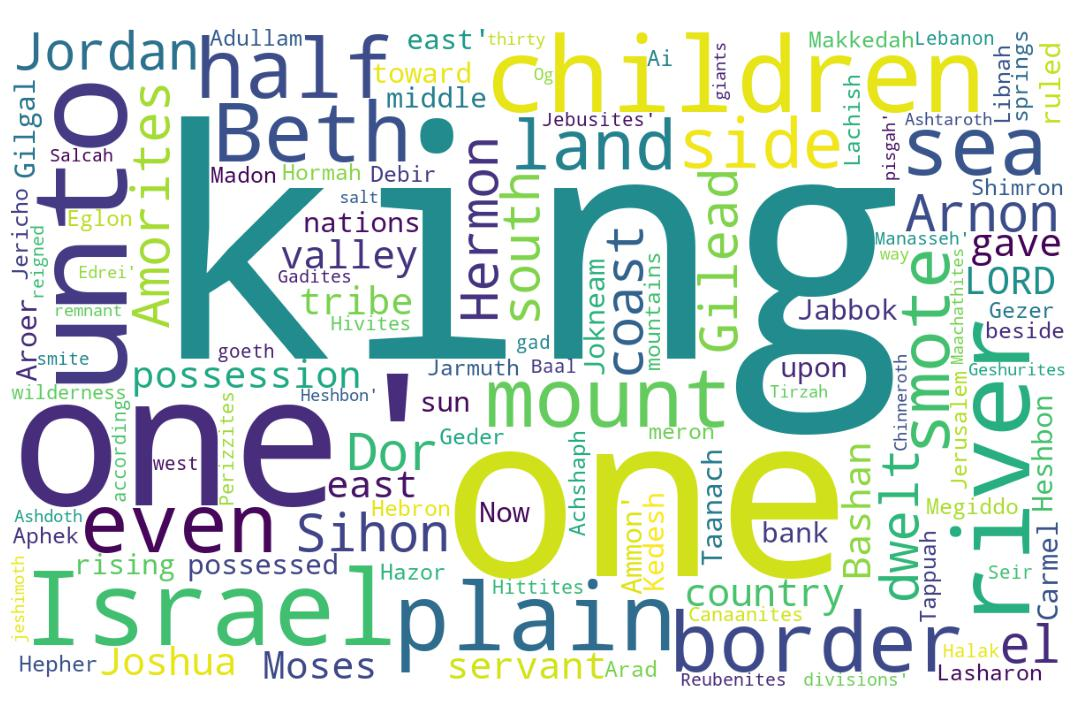
\includegraphics[width=\linewidth]{06OT-Joshua/Joshua12-WordCloud.jpg}
  \caption{Joshua 12 Word Cloud}
  \label{fig:Joshua 12 Word Cloud}
\end{figure}

\marginpar{\scriptsize \centering \fcolorbox{bone}{lime}{\textbf{A RECAP}}\\ (Joshua 12)

\begin{compactenum}[I.][8]

	\item \textbf{These} Ones Defeated  \index[scripture]{Joshua!Jsh 12:01}  (Jsh 12:1, 7) 
	\item \textbf{Tribes} On the Other Side  \index[scripture]{Joshua!Jsh 12:06}  (Jsh 12:6) 
	\item The \textbf{Terrain}  \index[scripture]{Joshua!Jsh 12:08}  (Jsh 12:8) 	
	\item \textbf{Thoughtful} Reflection -- take some time to consider the victories Gad has wrought in your life %\index[scripture]{Joshua!Jsh 12:24}  (Jsh 12:24) 
	\item \textbf{Thirty-One} Kings  \index[scripture]{Joshua!Jsh 12:10-24}  (Jsh 12:10-24) 

\end{compactenum}}





\footnote{\textcolor[cmyk]{0.99998,1,0,0}{\hyperlink{TOC}{Return to end of Table of Contents.}}}\footnote{\href{https://audiobible.com/bible/joshua_12.html}{\textcolor[cmyk]{0.99998,1,0,0}{Joshua 12 Audio}}}\textcolor[cmyk]{0.99998,1,0,0}{Now \fcolorbox{bone}{lime}{these} \emph{are} the kings of the land, which the children of Israel smote, and possessed their land on the other side Jordan toward the rising of the sun, from the river Arnon unto mount Hermon, and all the plain on the east:}
[2] \textcolor[cmyk]{0.99998,1,0,0}{Sihon king of the Amorites, who dwelt in Heshbon, \emph{and} ruled from Aroer, which \emph{is} upon the bank of the river Arnon, and from the middle of the river, and from half Gilead, even unto the river Jabbok, \emph{which} \emph{is} the border of the children of Ammon;}
[3] \textcolor[cmyk]{0.99998,1,0,0}{And from the plain to the sea of Chinneroth on the east, and unto the sea of the plain, \emph{even} the salt sea on the east, the way to Beth-jeshimoth; and from the south, under Ashdoth-pisgah:}\\
\\
\textcolor[cmyk]{0.99998,1,0,0}{And the coast of Og king of Bashan, \emph{which} \emph{was} of the remnant of the giants, that dwelt at Ashtaroth and at Edrei,}
[5] \textcolor[cmyk]{0.99998,1,0,0}{And reigned in mount Hermon, and in Salcah, and in all Bashan, unto the border of the Geshurites and the Maachathites, and half Gilead, the border of Sihon king of Heshbon.}
[6] \textcolor[cmyk]{0.99998,1,0,0}{Them did Moses the servant of the LORD and the children of Israel smite: and Moses the servant of the LORD gave it \emph{for} a possession unto the Reubenites, and the Gadites, and the half \fcolorbox{bone}{lime}{tribe} of Manasseh.}
[7] \textcolor[cmyk]{0.99998,1,0,0}{And \fcolorbox{bone}{lime}{these} \emph{are} the kings of the country which Joshua and the children of Israel smote on this side Jordan on the west, from Baal-gad in the valley of Lebanon even unto the mount Halak, that goeth up to Seir; which Joshua gave unto the tribes of Israel \emph{for} a possession according to their divisions;}
[8] \textcolor[cmyk]{0.99998,1,0,0}{In the \fcolorbox{bone}{lime}{mountains}, and in the \fcolorbox{bone}{lime}{valleys}, and in the \fcolorbox{bone}{lime}{plains}, and in the \fcolorbox{bone}{lime}{springs}, and in the \fcolorbox{bone}{lime}{wilderness}, and in the \fcolorbox{bone}{lime}{south country}; the Hittites, the Amorites, and the Canaanites, the Perizzites, the Hivites, and the Jebusites:}\\
\\
\textcolor[cmyk]{0.99998,1,0,0}{The king of Jericho, one; the king of Ai, which \emph{is} beside Beth-el, one;}
[10] \textcolor[cmyk]{0.99998,1,0,0}{The king of Jerusalem, one; the king of Hebron, one;}
[11] \textcolor[cmyk]{0.99998,1,0,0}{The king of Jarmuth, one; the king of Lachish, one;}
[12] \textcolor[cmyk]{0.99998,1,0,0}{The king of Eglon, one; the king of Gezer, one;}
[13] \textcolor[cmyk]{0.99998,1,0,0}{The king of Debir, one; the king of Geder, one;}
[14] \textcolor[cmyk]{0.99998,1,0,0}{The king of Hormah, one; the king of Arad, one;}
[15] \textcolor[cmyk]{0.99998,1,0,0}{The king of Libnah, one; the king of Adullam, one;}
[16] \textcolor[cmyk]{0.99998,1,0,0}{The king of Makkedah, one; the king of Beth-el, one;}
[17] \textcolor[cmyk]{0.99998,1,0,0}{The king of Tappuah, one; the king of Hepher, one;}
[18] \textcolor[cmyk]{0.99998,1,0,0}{The king of Aphek, one; the king of Lasharon, one;}
[19] \textcolor[cmyk]{0.99998,1,0,0}{The king of Madon, one; the king of Hazor, one;}
[20] \textcolor[cmyk]{0.99998,1,0,0}{The king of Shimron-meron, one; the king of Achshaph, one;}
[21] \textcolor[cmyk]{0.99998,1,0,0}{The king of Taanach, one; the king of Megiddo, one;}
[22] \textcolor[cmyk]{0.99998,1,0,0}{The king of Kedesh, one; the king of Jokneam of Carmel, one;}
[23] \textcolor[cmyk]{0.99998,1,0,0}{The king of Dor in the coast of Dor, one; the king of the nations of Gilgal, one;}
[24] \textcolor[cmyk]{0.99998,1,0,0}{The king of Tirzah, one: all the kings thirty and one.}
\index[NWIV]{43!Joshua!Jos 12:1}\index[AWIP]{Now!Joshua!Jos 12:1}\index[AWIP]{these!Joshua!Jos 12:1}\index[AWIP]{\emph{are}!Joshua!Jos 12:1}\index[AWIP]{the!Joshua!Jos 12:1}\index[AWIP]{the!Joshua!Jos 12:1 (2)}\index[AWIP]{the!Joshua!Jos 12:1 (3)}\index[AWIP]{the!Joshua!Jos 12:1 (4)}\index[AWIP]{the!Joshua!Jos 12:1 (5)}\index[AWIP]{the!Joshua!Jos 12:1 (6)}\index[AWIP]{the!Joshua!Jos 12:1 (7)}\index[AWIP]{the!Joshua!Jos 12:1 (8)}\index[AWIP]{the!Joshua!Jos 12:1 (9)}\index[AWIP]{kings!Joshua!Jos 12:1}\index[AWIP]{of!Joshua!Jos 12:1}\index[AWIP]{of!Joshua!Jos 12:1 (2)}\index[AWIP]{of!Joshua!Jos 12:1 (3)}\index[AWIP]{land!Joshua!Jos 12:1}\index[AWIP]{land!Joshua!Jos 12:1 (2)}\index[AWIP]{which!Joshua!Jos 12:1}\index[AWIP]{children!Joshua!Jos 12:1}\index[AWIP]{Israel!Joshua!Jos 12:1}\index[AWIP]{smote!Joshua!Jos 12:1}\index[AWIP]{and!Joshua!Jos 12:1}\index[AWIP]{and!Joshua!Jos 12:1 (2)}\index[AWIP]{possessed!Joshua!Jos 12:1}\index[AWIP]{their!Joshua!Jos 12:1}\index[AWIP]{on!Joshua!Jos 12:1}\index[AWIP]{on!Joshua!Jos 12:1 (2)}\index[AWIP]{other!Joshua!Jos 12:1}\index[AWIP]{side!Joshua!Jos 12:1}\index[AWIP]{Jordan!Joshua!Jos 12:1}\index[AWIP]{toward!Joshua!Jos 12:1}\index[AWIP]{rising!Joshua!Jos 12:1}\index[AWIP]{sun!Joshua!Jos 12:1}\index[AWIP]{from!Joshua!Jos 12:1}\index[AWIP]{river!Joshua!Jos 12:1}\index[AWIP]{Arnon!Joshua!Jos 12:1}\index[AWIP]{unto!Joshua!Jos 12:1}\index[AWIP]{mount!Joshua!Jos 12:1}\index[AWIP]{Hermon!Joshua!Jos 12:1}\index[AWIP]{all!Joshua!Jos 12:1}\index[AWIP]{plain!Joshua!Jos 12:1}\index[AWIP]{east!Joshua!Jos 12:1}\index[AWIP]{\emph{are}!Joshua!Jos 12:1}

\index[NWIV]{47!Joshua!Jos 12:2}\index[AWIP]{Sihon!Joshua!Jos 12:2}\index[AWIP]{king!Joshua!Jos 12:2}\index[AWIP]{of!Joshua!Jos 12:2}\index[AWIP]{of!Joshua!Jos 12:2 (2)}\index[AWIP]{of!Joshua!Jos 12:2 (3)}\index[AWIP]{of!Joshua!Jos 12:2 (4)}\index[AWIP]{of!Joshua!Jos 12:2 (5)}\index[AWIP]{the!Joshua!Jos 12:2}\index[AWIP]{the!Joshua!Jos 12:2 (2)}\index[AWIP]{the!Joshua!Jos 12:2 (3)}\index[AWIP]{the!Joshua!Jos 12:2 (4)}\index[AWIP]{the!Joshua!Jos 12:2 (5)}\index[AWIP]{the!Joshua!Jos 12:2 (6)}\index[AWIP]{the!Joshua!Jos 12:2 (7)}\index[AWIP]{the!Joshua!Jos 12:2 (8)}\index[AWIP]{Amorites!Joshua!Jos 12:2}\index[AWIP]{who!Joshua!Jos 12:2}\index[AWIP]{dwelt!Joshua!Jos 12:2}\index[AWIP]{in!Joshua!Jos 12:2}\index[AWIP]{Heshbon!Joshua!Jos 12:2}\index[AWIP]{\emph{and}!Joshua!Jos 12:2}\index[AWIP]{ruled!Joshua!Jos 12:2}\index[AWIP]{from!Joshua!Jos 12:2}\index[AWIP]{from!Joshua!Jos 12:2 (2)}\index[AWIP]{from!Joshua!Jos 12:2 (3)}\index[AWIP]{Aroer!Joshua!Jos 12:2}\index[AWIP]{which!Joshua!Jos 12:2}\index[AWIP]{\emph{is}!Joshua!Jos 12:2}\index[AWIP]{\emph{is}!Joshua!Jos 12:2 (2)}\index[AWIP]{upon!Joshua!Jos 12:2}\index[AWIP]{bank!Joshua!Jos 12:2}\index[AWIP]{river!Joshua!Jos 12:2}\index[AWIP]{river!Joshua!Jos 12:2 (2)}\index[AWIP]{river!Joshua!Jos 12:2 (3)}\index[AWIP]{Arnon!Joshua!Jos 12:2}\index[AWIP]{and!Joshua!Jos 12:2}\index[AWIP]{and!Joshua!Jos 12:2 (2)}\index[AWIP]{middle!Joshua!Jos 12:2}\index[AWIP]{half!Joshua!Jos 12:2}\index[AWIP]{Gilead!Joshua!Jos 12:2}\index[AWIP]{even!Joshua!Jos 12:2}\index[AWIP]{unto!Joshua!Jos 12:2}\index[AWIP]{Jabbok!Joshua!Jos 12:2}\index[AWIP]{\emph{which}!Joshua!Jos 12:2}\index[AWIP]{border!Joshua!Jos 12:2}\index[AWIP]{children!Joshua!Jos 12:2}\index[AWIP]{Ammon!Joshua!Jos 12:2}\index[AWIP]{\emph{and}!Joshua!Jos 12:2}\index[AWIP]{\emph{is}!Joshua!Jos 12:2}\index[AWIP]{\emph{is}!Joshua!Jos 12:2 (2)}\index[AWIP]{\emph{which}!Joshua!Jos 12:2}

\index[NWIV]{36!Joshua!Jos 12:3}\index[AWIP]{And!Joshua!Jos 12:3}\index[AWIP]{from!Joshua!Jos 12:3}\index[AWIP]{from!Joshua!Jos 12:3 (2)}\index[AWIP]{the!Joshua!Jos 12:3}\index[AWIP]{the!Joshua!Jos 12:3 (2)}\index[AWIP]{the!Joshua!Jos 12:3 (3)}\index[AWIP]{the!Joshua!Jos 12:3 (4)}\index[AWIP]{the!Joshua!Jos 12:3 (5)}\index[AWIP]{the!Joshua!Jos 12:3 (6)}\index[AWIP]{the!Joshua!Jos 12:3 (7)}\index[AWIP]{the!Joshua!Jos 12:3 (8)}\index[AWIP]{the!Joshua!Jos 12:3 (9)}\index[AWIP]{plain!Joshua!Jos 12:3}\index[AWIP]{plain!Joshua!Jos 12:3 (2)}\index[AWIP]{to!Joshua!Jos 12:3}\index[AWIP]{to!Joshua!Jos 12:3 (2)}\index[AWIP]{sea!Joshua!Jos 12:3}\index[AWIP]{sea!Joshua!Jos 12:3 (2)}\index[AWIP]{sea!Joshua!Jos 12:3 (3)}\index[AWIP]{of!Joshua!Jos 12:3}\index[AWIP]{of!Joshua!Jos 12:3 (2)}\index[AWIP]{Chinneroth!Joshua!Jos 12:3}\index[AWIP]{on!Joshua!Jos 12:3}\index[AWIP]{on!Joshua!Jos 12:3 (2)}\index[AWIP]{east!Joshua!Jos 12:3}\index[AWIP]{east!Joshua!Jos 12:3 (2)}\index[AWIP]{and!Joshua!Jos 12:3}\index[AWIP]{and!Joshua!Jos 12:3 (2)}\index[AWIP]{unto!Joshua!Jos 12:3}\index[AWIP]{\emph{even}!Joshua!Jos 12:3}\index[AWIP]{salt!Joshua!Jos 12:3}\index[AWIP]{way!Joshua!Jos 12:3}\index[AWIP]{Beth-jeshimoth!Joshua!Jos 12:3}\index[AWIP]{south!Joshua!Jos 12:3}\index[AWIP]{under!Joshua!Jos 12:3}\index[AWIP]{Ashdoth-pisgah!Joshua!Jos 12:3}\index[AWIP]{\emph{even}!Joshua!Jos 12:3}

\index[NWIV]{23!Joshua!Jos 12:4}\index[AWIP]{And!Joshua!Jos 12:4}\index[AWIP]{the!Joshua!Jos 12:4}\index[AWIP]{the!Joshua!Jos 12:4 (2)}\index[AWIP]{the!Joshua!Jos 12:4 (3)}\index[AWIP]{coast!Joshua!Jos 12:4}\index[AWIP]{of!Joshua!Jos 12:4}\index[AWIP]{of!Joshua!Jos 12:4 (2)}\index[AWIP]{of!Joshua!Jos 12:4 (3)}\index[AWIP]{of!Joshua!Jos 12:4 (4)}\index[AWIP]{Og!Joshua!Jos 12:4}\index[AWIP]{king!Joshua!Jos 12:4}\index[AWIP]{Bashan!Joshua!Jos 12:4}\index[AWIP]{\emph{which}!Joshua!Jos 12:4}\index[AWIP]{\emph{was}!Joshua!Jos 12:4}\index[AWIP]{remnant!Joshua!Jos 12:4}\index[AWIP]{giants!Joshua!Jos 12:4}\index[AWIP]{that!Joshua!Jos 12:4}\index[AWIP]{dwelt!Joshua!Jos 12:4}\index[AWIP]{at!Joshua!Jos 12:4}\index[AWIP]{at!Joshua!Jos 12:4 (2)}\index[AWIP]{Ashtaroth!Joshua!Jos 12:4}\index[AWIP]{and!Joshua!Jos 12:4}\index[AWIP]{Edrei!Joshua!Jos 12:4}\index[AWIP]{\emph{which}!Joshua!Jos 12:4}\index[AWIP]{\emph{was}!Joshua!Jos 12:4}

\index[NWIV]{31!Joshua!Jos 12:5}\index[AWIP]{And!Joshua!Jos 12:5}\index[AWIP]{reigned!Joshua!Jos 12:5}\index[AWIP]{in!Joshua!Jos 12:5}\index[AWIP]{in!Joshua!Jos 12:5 (2)}\index[AWIP]{in!Joshua!Jos 12:5 (3)}\index[AWIP]{mount!Joshua!Jos 12:5}\index[AWIP]{Hermon!Joshua!Jos 12:5}\index[AWIP]{and!Joshua!Jos 12:5}\index[AWIP]{and!Joshua!Jos 12:5 (2)}\index[AWIP]{and!Joshua!Jos 12:5 (3)}\index[AWIP]{and!Joshua!Jos 12:5 (4)}\index[AWIP]{Salcah!Joshua!Jos 12:5}\index[AWIP]{all!Joshua!Jos 12:5}\index[AWIP]{Bashan!Joshua!Jos 12:5}\index[AWIP]{unto!Joshua!Jos 12:5}\index[AWIP]{the!Joshua!Jos 12:5}\index[AWIP]{the!Joshua!Jos 12:5 (2)}\index[AWIP]{the!Joshua!Jos 12:5 (3)}\index[AWIP]{the!Joshua!Jos 12:5 (4)}\index[AWIP]{border!Joshua!Jos 12:5}\index[AWIP]{border!Joshua!Jos 12:5 (2)}\index[AWIP]{of!Joshua!Jos 12:5}\index[AWIP]{of!Joshua!Jos 12:5 (2)}\index[AWIP]{of!Joshua!Jos 12:5 (3)}\index[AWIP]{Geshurites!Joshua!Jos 12:5}\index[AWIP]{Maachathites!Joshua!Jos 12:5}\index[AWIP]{half!Joshua!Jos 12:5}\index[AWIP]{Gilead!Joshua!Jos 12:5}\index[AWIP]{Sihon!Joshua!Jos 12:5}\index[AWIP]{king!Joshua!Jos 12:5}\index[AWIP]{Heshbon!Joshua!Jos 12:5}

\index[NWIV]{38!Joshua!Jos 12:6}\index[AWIP]{Them!Joshua!Jos 12:6}\index[AWIP]{did!Joshua!Jos 12:6}\index[AWIP]{Moses!Joshua!Jos 12:6}\index[AWIP]{Moses!Joshua!Jos 12:6 (2)}\index[AWIP]{the!Joshua!Jos 12:6}\index[AWIP]{the!Joshua!Jos 12:6 (2)}\index[AWIP]{the!Joshua!Jos 12:6 (3)}\index[AWIP]{the!Joshua!Jos 12:6 (4)}\index[AWIP]{the!Joshua!Jos 12:6 (5)}\index[AWIP]{the!Joshua!Jos 12:6 (6)}\index[AWIP]{the!Joshua!Jos 12:6 (7)}\index[AWIP]{the!Joshua!Jos 12:6 (8)}\index[AWIP]{servant!Joshua!Jos 12:6}\index[AWIP]{servant!Joshua!Jos 12:6 (2)}\index[AWIP]{of!Joshua!Jos 12:6}\index[AWIP]{of!Joshua!Jos 12:6 (2)}\index[AWIP]{of!Joshua!Jos 12:6 (3)}\index[AWIP]{of!Joshua!Jos 12:6 (4)}\index[AWIP]{LORD!Joshua!Jos 12:6}\index[AWIP]{LORD!Joshua!Jos 12:6 (2)}\index[AWIP]{and!Joshua!Jos 12:6}\index[AWIP]{and!Joshua!Jos 12:6 (2)}\index[AWIP]{and!Joshua!Jos 12:6 (3)}\index[AWIP]{and!Joshua!Jos 12:6 (4)}\index[AWIP]{children!Joshua!Jos 12:6}\index[AWIP]{Israel!Joshua!Jos 12:6}\index[AWIP]{smite!Joshua!Jos 12:6}\index[AWIP]{gave!Joshua!Jos 12:6}\index[AWIP]{it!Joshua!Jos 12:6}\index[AWIP]{\emph{for}!Joshua!Jos 12:6}\index[AWIP]{a!Joshua!Jos 12:6}\index[AWIP]{possession!Joshua!Jos 12:6}\index[AWIP]{unto!Joshua!Jos 12:6}\index[AWIP]{Reubenites!Joshua!Jos 12:6}\index[AWIP]{Gadites!Joshua!Jos 12:6}\index[AWIP]{half!Joshua!Jos 12:6}\index[AWIP]{tribe!Joshua!Jos 12:6}\index[AWIP]{Manasseh!Joshua!Jos 12:6}\index[AWIP]{\emph{for}!Joshua!Jos 12:6}

\index[NWIV]{55!Joshua!Jos 12:7}\index[AWIP]{And!Joshua!Jos 12:7}\index[AWIP]{these!Joshua!Jos 12:7}\index[AWIP]{\emph{are}!Joshua!Jos 12:7}\index[AWIP]{the!Joshua!Jos 12:7}\index[AWIP]{the!Joshua!Jos 12:7 (2)}\index[AWIP]{the!Joshua!Jos 12:7 (3)}\index[AWIP]{the!Joshua!Jos 12:7 (4)}\index[AWIP]{the!Joshua!Jos 12:7 (5)}\index[AWIP]{the!Joshua!Jos 12:7 (6)}\index[AWIP]{the!Joshua!Jos 12:7 (7)}\index[AWIP]{kings!Joshua!Jos 12:7}\index[AWIP]{of!Joshua!Jos 12:7}\index[AWIP]{of!Joshua!Jos 12:7 (2)}\index[AWIP]{of!Joshua!Jos 12:7 (3)}\index[AWIP]{of!Joshua!Jos 12:7 (4)}\index[AWIP]{country!Joshua!Jos 12:7}\index[AWIP]{which!Joshua!Jos 12:7}\index[AWIP]{which!Joshua!Jos 12:7 (2)}\index[AWIP]{Joshua!Joshua!Jos 12:7}\index[AWIP]{Joshua!Joshua!Jos 12:7 (2)}\index[AWIP]{and!Joshua!Jos 12:7}\index[AWIP]{children!Joshua!Jos 12:7}\index[AWIP]{Israel!Joshua!Jos 12:7}\index[AWIP]{Israel!Joshua!Jos 12:7 (2)}\index[AWIP]{smote!Joshua!Jos 12:7}\index[AWIP]{on!Joshua!Jos 12:7}\index[AWIP]{on!Joshua!Jos 12:7 (2)}\index[AWIP]{this!Joshua!Jos 12:7}\index[AWIP]{side!Joshua!Jos 12:7}\index[AWIP]{Jordan!Joshua!Jos 12:7}\index[AWIP]{west!Joshua!Jos 12:7}\index[AWIP]{from!Joshua!Jos 12:7}\index[AWIP]{Baal-gad!Joshua!Jos 12:7}\index[AWIP]{in!Joshua!Jos 12:7}\index[AWIP]{valley!Joshua!Jos 12:7}\index[AWIP]{Lebanon!Joshua!Jos 12:7}\index[AWIP]{even!Joshua!Jos 12:7}\index[AWIP]{unto!Joshua!Jos 12:7}\index[AWIP]{unto!Joshua!Jos 12:7 (2)}\index[AWIP]{mount!Joshua!Jos 12:7}\index[AWIP]{Halak!Joshua!Jos 12:7}\index[AWIP]{that!Joshua!Jos 12:7}\index[AWIP]{goeth!Joshua!Jos 12:7}\index[AWIP]{up!Joshua!Jos 12:7}\index[AWIP]{to!Joshua!Jos 12:7}\index[AWIP]{to!Joshua!Jos 12:7 (2)}\index[AWIP]{Seir!Joshua!Jos 12:7}\index[AWIP]{gave!Joshua!Jos 12:7}\index[AWIP]{tribes!Joshua!Jos 12:7}\index[AWIP]{\emph{for}!Joshua!Jos 12:7}\index[AWIP]{a!Joshua!Jos 12:7}\index[AWIP]{possession!Joshua!Jos 12:7}\index[AWIP]{according!Joshua!Jos 12:7}\index[AWIP]{their!Joshua!Jos 12:7}\index[AWIP]{divisions!Joshua!Jos 12:7}\index[AWIP]{\emph{are}!Joshua!Jos 12:7}\index[AWIP]{\emph{for}!Joshua!Jos 12:7}

\index[NWIV]{38!Joshua!Jos 12:8}\index[AWIP]{In!Joshua!Jos 12:8}\index[AWIP]{the!Joshua!Jos 12:8}\index[AWIP]{the!Joshua!Jos 12:8 (2)}\index[AWIP]{the!Joshua!Jos 12:8 (3)}\index[AWIP]{the!Joshua!Jos 12:8 (4)}\index[AWIP]{the!Joshua!Jos 12:8 (5)}\index[AWIP]{the!Joshua!Jos 12:8 (6)}\index[AWIP]{the!Joshua!Jos 12:8 (7)}\index[AWIP]{the!Joshua!Jos 12:8 (8)}\index[AWIP]{the!Joshua!Jos 12:8 (9)}\index[AWIP]{the!Joshua!Jos 12:8 (10)}\index[AWIP]{the!Joshua!Jos 12:8 (11)}\index[AWIP]{the!Joshua!Jos 12:8 (12)}\index[AWIP]{mountains!Joshua!Jos 12:8}\index[AWIP]{and!Joshua!Jos 12:8}\index[AWIP]{and!Joshua!Jos 12:8 (2)}\index[AWIP]{and!Joshua!Jos 12:8 (3)}\index[AWIP]{and!Joshua!Jos 12:8 (4)}\index[AWIP]{and!Joshua!Jos 12:8 (5)}\index[AWIP]{and!Joshua!Jos 12:8 (6)}\index[AWIP]{and!Joshua!Jos 12:8 (7)}\index[AWIP]{in!Joshua!Jos 12:8}\index[AWIP]{in!Joshua!Jos 12:8 (2)}\index[AWIP]{in!Joshua!Jos 12:8 (3)}\index[AWIP]{in!Joshua!Jos 12:8 (4)}\index[AWIP]{in!Joshua!Jos 12:8 (5)}\index[AWIP]{valleys!Joshua!Jos 12:8}\index[AWIP]{plains!Joshua!Jos 12:8}\index[AWIP]{springs!Joshua!Jos 12:8}\index[AWIP]{wilderness!Joshua!Jos 12:8}\index[AWIP]{south!Joshua!Jos 12:8}\index[AWIP]{country!Joshua!Jos 12:8}\index[AWIP]{Hittites!Joshua!Jos 12:8}\index[AWIP]{Amorites!Joshua!Jos 12:8}\index[AWIP]{Canaanites!Joshua!Jos 12:8}\index[AWIP]{Perizzites!Joshua!Jos 12:8}\index[AWIP]{Hivites!Joshua!Jos 12:8}\index[AWIP]{Jebusites!Joshua!Jos 12:8}

\index[NWIV]{14!Joshua!Jos 12:9}\index[AWIP]{The!Joshua!Jos 12:9}\index[AWIP]{king!Joshua!Jos 12:9}\index[AWIP]{king!Joshua!Jos 12:9 (2)}\index[AWIP]{of!Joshua!Jos 12:9}\index[AWIP]{of!Joshua!Jos 12:9 (2)}\index[AWIP]{Jericho!Joshua!Jos 12:9}\index[AWIP]{one!Joshua!Jos 12:9}\index[AWIP]{one!Joshua!Jos 12:9 (2)}\index[AWIP]{the!Joshua!Jos 12:9}\index[AWIP]{Ai!Joshua!Jos 12:9}\index[AWIP]{which!Joshua!Jos 12:9}\index[AWIP]{\emph{is}!Joshua!Jos 12:9}\index[AWIP]{beside!Joshua!Jos 12:9}\index[AWIP]{Beth-el!Joshua!Jos 12:9}\index[AWIP]{\emph{is}!Joshua!Jos 12:9}

\index[NWIV]{10!Joshua!Jos 12:10}\index[AWIP]{The!Joshua!Jos 12:10}\index[AWIP]{king!Joshua!Jos 12:10}\index[AWIP]{king!Joshua!Jos 12:10 (2)}\index[AWIP]{of!Joshua!Jos 12:10}\index[AWIP]{of!Joshua!Jos 12:10 (2)}\index[AWIP]{Jerusalem!Joshua!Jos 12:10}\index[AWIP]{one!Joshua!Jos 12:10}\index[AWIP]{one!Joshua!Jos 12:10 (2)}\index[AWIP]{the!Joshua!Jos 12:10}\index[AWIP]{Hebron!Joshua!Jos 12:10}

\index[NWIV]{10!Joshua!Jos 12:11}\index[AWIP]{The!Joshua!Jos 12:11}\index[AWIP]{king!Joshua!Jos 12:11}\index[AWIP]{king!Joshua!Jos 12:11 (2)}\index[AWIP]{of!Joshua!Jos 12:11}\index[AWIP]{of!Joshua!Jos 12:11 (2)}\index[AWIP]{Jarmuth!Joshua!Jos 12:11}\index[AWIP]{one!Joshua!Jos 12:11}\index[AWIP]{one!Joshua!Jos 12:11 (2)}\index[AWIP]{the!Joshua!Jos 12:11}\index[AWIP]{Lachish!Joshua!Jos 12:11}

\index[NWIV]{10!Joshua!Jos 12:12}\index[AWIP]{The!Joshua!Jos 12:12}\index[AWIP]{king!Joshua!Jos 12:12}\index[AWIP]{king!Joshua!Jos 12:12 (2)}\index[AWIP]{of!Joshua!Jos 12:12}\index[AWIP]{of!Joshua!Jos 12:12 (2)}\index[AWIP]{Eglon!Joshua!Jos 12:12}\index[AWIP]{one!Joshua!Jos 12:12}\index[AWIP]{one!Joshua!Jos 12:12 (2)}\index[AWIP]{the!Joshua!Jos 12:12}\index[AWIP]{Gezer!Joshua!Jos 12:12}

\index[NWIV]{10!Joshua!Jos 12:13}\index[AWIP]{The!Joshua!Jos 12:13}\index[AWIP]{king!Joshua!Jos 12:13}\index[AWIP]{king!Joshua!Jos 12:13 (2)}\index[AWIP]{of!Joshua!Jos 12:13}\index[AWIP]{of!Joshua!Jos 12:13 (2)}\index[AWIP]{Debir!Joshua!Jos 12:13}\index[AWIP]{one!Joshua!Jos 12:13}\index[AWIP]{one!Joshua!Jos 12:13 (2)}\index[AWIP]{the!Joshua!Jos 12:13}\index[AWIP]{Geder!Joshua!Jos 12:13}

\index[NWIV]{10!Joshua!Jos 12:14}\index[AWIP]{The!Joshua!Jos 12:14}\index[AWIP]{king!Joshua!Jos 12:14}\index[AWIP]{king!Joshua!Jos 12:14 (2)}\index[AWIP]{of!Joshua!Jos 12:14}\index[AWIP]{of!Joshua!Jos 12:14 (2)}\index[AWIP]{Hormah!Joshua!Jos 12:14}\index[AWIP]{one!Joshua!Jos 12:14}\index[AWIP]{one!Joshua!Jos 12:14 (2)}\index[AWIP]{the!Joshua!Jos 12:14}\index[AWIP]{Arad!Joshua!Jos 12:14}

\index[NWIV]{10!Joshua!Jos 12:15}\index[AWIP]{The!Joshua!Jos 12:15}\index[AWIP]{king!Joshua!Jos 12:15}\index[AWIP]{king!Joshua!Jos 12:15 (2)}\index[AWIP]{of!Joshua!Jos 12:15}\index[AWIP]{of!Joshua!Jos 12:15 (2)}\index[AWIP]{Libnah!Joshua!Jos 12:15}\index[AWIP]{one!Joshua!Jos 12:15}\index[AWIP]{one!Joshua!Jos 12:15 (2)}\index[AWIP]{the!Joshua!Jos 12:15}\index[AWIP]{Adullam!Joshua!Jos 12:15}

\index[NWIV]{10!Joshua!Jos 12:16}\index[AWIP]{The!Joshua!Jos 12:16}\index[AWIP]{king!Joshua!Jos 12:16}\index[AWIP]{king!Joshua!Jos 12:16 (2)}\index[AWIP]{of!Joshua!Jos 12:16}\index[AWIP]{of!Joshua!Jos 12:16 (2)}\index[AWIP]{Makkedah!Joshua!Jos 12:16}\index[AWIP]{one!Joshua!Jos 12:16}\index[AWIP]{one!Joshua!Jos 12:16 (2)}\index[AWIP]{the!Joshua!Jos 12:16}\index[AWIP]{Beth-el!Joshua!Jos 12:16}

\index[NWIV]{10!Joshua!Jos 12:17}\index[AWIP]{The!Joshua!Jos 12:17}\index[AWIP]{king!Joshua!Jos 12:17}\index[AWIP]{king!Joshua!Jos 12:17 (2)}\index[AWIP]{of!Joshua!Jos 12:17}\index[AWIP]{of!Joshua!Jos 12:17 (2)}\index[AWIP]{Tappuah!Joshua!Jos 12:17}\index[AWIP]{one!Joshua!Jos 12:17}\index[AWIP]{one!Joshua!Jos 12:17 (2)}\index[AWIP]{the!Joshua!Jos 12:17}\index[AWIP]{Hepher!Joshua!Jos 12:17}

\index[NWIV]{10!Joshua!Jos 12:18}\index[AWIP]{The!Joshua!Jos 12:18}\index[AWIP]{king!Joshua!Jos 12:18}\index[AWIP]{king!Joshua!Jos 12:18 (2)}\index[AWIP]{of!Joshua!Jos 12:18}\index[AWIP]{of!Joshua!Jos 12:18 (2)}\index[AWIP]{Aphek!Joshua!Jos 12:18}\index[AWIP]{one!Joshua!Jos 12:18}\index[AWIP]{one!Joshua!Jos 12:18 (2)}\index[AWIP]{the!Joshua!Jos 12:18}\index[AWIP]{Lasharon!Joshua!Jos 12:18}

\index[NWIV]{10!Joshua!Jos 12:19}\index[AWIP]{The!Joshua!Jos 12:19}\index[AWIP]{king!Joshua!Jos 12:19}\index[AWIP]{king!Joshua!Jos 12:19 (2)}\index[AWIP]{of!Joshua!Jos 12:19}\index[AWIP]{of!Joshua!Jos 12:19 (2)}\index[AWIP]{Madon!Joshua!Jos 12:19}\index[AWIP]{one!Joshua!Jos 12:19}\index[AWIP]{one!Joshua!Jos 12:19 (2)}\index[AWIP]{the!Joshua!Jos 12:19}\index[AWIP]{Hazor!Joshua!Jos 12:19}

\index[NWIV]{10!Joshua!Jos 12:20}\index[AWIP]{The!Joshua!Jos 12:20}\index[AWIP]{king!Joshua!Jos 12:20}\index[AWIP]{king!Joshua!Jos 12:20 (2)}\index[AWIP]{of!Joshua!Jos 12:20}\index[AWIP]{of!Joshua!Jos 12:20 (2)}\index[AWIP]{Shimron-meron!Joshua!Jos 12:20}\index[AWIP]{one!Joshua!Jos 12:20}\index[AWIP]{one!Joshua!Jos 12:20 (2)}\index[AWIP]{the!Joshua!Jos 12:20}\index[AWIP]{Achshaph!Joshua!Jos 12:20}

\index[NWIV]{10!Joshua!Jos 12:21}\index[AWIP]{The!Joshua!Jos 12:21}\index[AWIP]{king!Joshua!Jos 12:21}\index[AWIP]{king!Joshua!Jos 12:21 (2)}\index[AWIP]{of!Joshua!Jos 12:21}\index[AWIP]{of!Joshua!Jos 12:21 (2)}\index[AWIP]{Taanach!Joshua!Jos 12:21}\index[AWIP]{one!Joshua!Jos 12:21}\index[AWIP]{one!Joshua!Jos 12:21 (2)}\index[AWIP]{the!Joshua!Jos 12:21}\index[AWIP]{Megiddo!Joshua!Jos 12:21}

\index[NWIV]{12!Joshua!Jos 12:22}\index[AWIP]{The!Joshua!Jos 12:22}\index[AWIP]{king!Joshua!Jos 12:22}\index[AWIP]{king!Joshua!Jos 12:22 (2)}\index[AWIP]{of!Joshua!Jos 12:22}\index[AWIP]{of!Joshua!Jos 12:22 (2)}\index[AWIP]{of!Joshua!Jos 12:22 (3)}\index[AWIP]{Kedesh!Joshua!Jos 12:22}\index[AWIP]{one!Joshua!Jos 12:22}\index[AWIP]{one!Joshua!Jos 12:22 (2)}\index[AWIP]{the!Joshua!Jos 12:22}\index[AWIP]{Jokneam!Joshua!Jos 12:22}\index[AWIP]{Carmel!Joshua!Jos 12:22}

\index[NWIV]{18!Joshua!Jos 12:23}\index[AWIP]{The!Joshua!Jos 12:23}\index[AWIP]{king!Joshua!Jos 12:23}\index[AWIP]{king!Joshua!Jos 12:23 (2)}\index[AWIP]{of!Joshua!Jos 12:23}\index[AWIP]{of!Joshua!Jos 12:23 (2)}\index[AWIP]{of!Joshua!Jos 12:23 (3)}\index[AWIP]{of!Joshua!Jos 12:23 (4)}\index[AWIP]{Dor!Joshua!Jos 12:23}\index[AWIP]{Dor!Joshua!Jos 12:23 (2)}\index[AWIP]{in!Joshua!Jos 12:23}\index[AWIP]{the!Joshua!Jos 12:23}\index[AWIP]{the!Joshua!Jos 12:23 (2)}\index[AWIP]{the!Joshua!Jos 12:23 (3)}\index[AWIP]{coast!Joshua!Jos 12:23}\index[AWIP]{one!Joshua!Jos 12:23}\index[AWIP]{one!Joshua!Jos 12:23 (2)}\index[AWIP]{nations!Joshua!Jos 12:23}\index[AWIP]{Gilgal!Joshua!Jos 12:23}

\index[NWIV]{11!Joshua!Jos 12:24}\index[AWIP]{The!Joshua!Jos 12:24}\index[AWIP]{king!Joshua!Jos 12:24}\index[AWIP]{of!Joshua!Jos 12:24}\index[AWIP]{Tirzah!Joshua!Jos 12:24}\index[AWIP]{one!Joshua!Jos 12:24}\index[AWIP]{one!Joshua!Jos 12:24 (2)}\index[AWIP]{all!Joshua!Jos 12:24}\index[AWIP]{the!Joshua!Jos 12:24}\index[AWIP]{kings!Joshua!Jos 12:24}\index[AWIP]{thirty!Joshua!Jos 12:24}\index[AWIP]{and!Joshua!Jos 12:24}


\section{Joshua 12 Outlines}

\subsection{My Outlines}

\subsubsection{A Recap}
\index[speaker]{Keith Anthony!Joshua 12 (A Recap}
\index[series]{Joshua (Keith Anthony)!Joshua 12 (A Recap)}
\index[date]{2018/03/08!Joshua 12 (A Recap) (Keith Anthony)}
\begin{compactenum}[I.]

	\item \textbf{These} Ones Defeated  \index[scripture]{Joshua!Jsh 12:01}  (Jsh 12:1, 7) 
	\item \textbf{Tribes} On the Other Side  \index[scripture]{Joshua!Jsh 12:06}  (Jsh 12:6) 
	\item The \textbf{Terrain}  \index[scripture]{Joshua!Jsh 12:08}  (Jsh 12:8) 
	\item \textbf{Thoughtful} Reflection -- take some time to consider the victories Gad has wrought in your life %\index[scripture]{Joshua!Jsh 12:24}  (Jsh 12:24) 
	\item \textbf{Thirty-One} Kings  \index[scripture]{Joshua!Jsh 12:10-24}  (Jsh 12:10-24) 

\end{compactenum}
\subsection{My Outlines from Others}


\section{Joshua 12 Comments}

\subsection{Numeric Nuggets}
\textbf{13: } The 13-character name ``Shimron-meron'' is found in the chapter (verse 20).
\subsection{Joshua 12 Repeated Phrases}


%%%%%%%%%%
%%%%%%%%%%
\normalsize
 
\begin{center}
\begin{longtable}{|p{3.0in}|p{0.5in}|}
\caption[Joshua 12 Repeated Phrases]{Joshua 12 Repeated Phrases}\label{table:Repeated Phrases Joshua 12} \\
\hline \multicolumn{1}{|c|}{\textbf{Phrase}} & \multicolumn{1}{c|}{\textbf{Frequency}} \\ \hline 
\endfirsthead
 
\multicolumn{2}{c}
{{\bfseries \tablename\ \thetable{} -- continued from previous page}} \\  
\hline \multicolumn{1}{|c|}{\textbf{Phrase}} & \multicolumn{1}{c|}{\textbf{Frequency}} \\ \hline 
\endhead
 
\hline \multicolumn{2}{c}{{ }} \\ \hline
\endfoot 
king of & 34\\ \hline 
The king & 16\\ \hline 
The king of & 16\\ \hline 
one the & 15\\ \hline 
one the king & 15\\ \hline 
one the king of & 15\\ \hline 
the king & 15\\ \hline 
the king of & 15\\ \hline 
of the & 14\\ \hline 
and in & 7\\ \hline 
and the & 7\\ \hline 
in the & 7\\ \hline 
unto the & 6\\ \hline 
on the & 5\\ \hline 
and in the & 5\\ \hline 
the children & 4\\ \hline 
the children of & 4\\ \hline 
children of & 4\\ \hline 
of Israel & 4\\ \hline 
from the & 4\\ \hline 
the river & 4\\ \hline 
the kings & 3\\ \hline 
the children of Israel & 3\\ \hline 
children of Israel & 3\\ \hline 
the plain & 3\\ \hline 
on the east & 3\\ \hline 
the east & 3\\ \hline 
and from & 3\\ \hline 
the border & 3\\ \hline 
the border of & 3\\ \hline 
border of & 3\\ \hline 
\end{longtable}
\end{center}



%%%%%%%%%%
%%%%%%%%%%



\section{Joshua 12 Statistics}

%%%%%%%%%%%%%%%%%%%%%%%%%%%
%%%%% Word Statistics
%%%%%%%%%%%%%%%%%%%%%%%%%%


\normalsize



\subsection{Chapter Word Statistics}


%%%%%%%%%%
%%%%%%%%%%
 
\begin{center}
\begin{longtable}{l|c|c|c|c}
\caption[Stats for Joshua 12]{Stats for Joshua 12} \label{table:Stats for Joshua 12} \\ 
\hline \multicolumn{1}{|c|}{\textbf{Verse(s)}} & \multicolumn{1}{|c|}{\textbf{Count}} & \multicolumn{1}{|c|}{\textbf{Unique}} & \multicolumn{1}{|c|}{\textbf{Italics}} & \multicolumn{1}{|c|}{\textbf{Uniq Italic}}  \\ \hline 
\endfirsthead
 
\multicolumn{5}{c}
{{\bfseries \tablename\ \thetable{} -- continued from previous page}} \\  
\hline \multicolumn{1}{|c|}{\textbf{Verse(s)}} & \multicolumn{1}{|c|}{\textbf{Count}} & \multicolumn{1}{|c|}{\textbf{Unique}} & \multicolumn{1}{|c|}{\textbf{Italics}} & \multicolumn{1}{|c|}{\textbf{Uniq Italic}}  \\ \hline 
\endhead
 
\hline \multicolumn{5}{|r|}{{Continued if needed}} \\ \hline
\endfoot 
1 & 43 & 30 & 1 & 1\\ \hline
2 & 47 & 30 & 4 & 3\\ \hline
3 & 36 & 19 & 1 & 1\\ \hline
4 & 23 & 17 & 2 & 2\\ \hline
5 & 31 & 20 & 0 & 0\\ \hline
6 & 38 & 22 & 1 & 1\\ \hline
7 & 55 & 40 & 2 & 2\\ \hline
8 & 38 & 17 & 0 & 0\\ \hline
9 & 14 & 11 & 1 & 1\\ \hline
10 & 10 & 7 & 0 & 0\\ \hline
11 & 10 & 7 & 0 & 0\\ \hline
12 & 10 & 7 & 0 & 0\\ \hline
13 & 10 & 7 & 0 & 0\\ \hline
14 & 10 & 7 & 0 & 0\\ \hline
15 & 10 & 7 & 0 & 0\\ \hline
16 & 10 & 7 & 0 & 0\\ \hline
17 & 10 & 7 & 0 & 0\\ \hline
18 & 10 & 7 & 0 & 0\\ \hline
19 & 10 & 7 & 0 & 0\\ \hline
20 & 10 & 7 & 0 & 0\\ \hline
21 & 10 & 7 & 0 & 0\\ \hline
22 & 12 & 8 & 0 & 0\\ \hline
23 & 18 & 10 & 0 & 0\\ \hline
24 & 11 & 10 & 0 & 0\\ \hline
\hline \hline
Total & 486 & 153 & 12 & 7



\end{longtable}
\end{center}

%%%%%%%%%%
%%%%%%%%%%
 
\subsection{Words by Frequency}

\begin{center}
\begin{longtable}{l|r}
\caption[Word Frequencies in Joshua 12]{Word Frequencies in Joshua 12} \label{table:WordsIn-Joshua-12} \\ 
\hline \multicolumn{1}{|c|}{\textbf{Word}} & \multicolumn{1}{c|}{\textbf{Frequency}} \\ \hline 
\endfirsthead
 
\multicolumn{2}{c}
{{\bfseries \tablename\ \thetable{} -- continued from previous page}} \\ 
\hline \multicolumn{1}{|c|}{\textbf{Word}} & \multicolumn{1}{c|}{\textbf{Frequency}} \\ \hline 
\endhead
 
\hline \multicolumn{2}{|r|}{{Continued if needed}} \\ \hline
\endfoot
 
\hline \hline
\endlastfoot
the & 78 \\ \hline
of & 59 \\ \hline
king & 34 \\ \hline
one & 32 \\ \hline
and & 24 \\ \hline
The & 16 \\ \hline
in & 11 \\ \hline
from & 7 \\ \hline
unto & 7 \\ \hline
on & 6 \\ \hline
which & 5 \\ \hline
children & 4 \\ \hline
Israel & 4 \\ \hline
river & 4 \\ \hline
And & 4 \\ \hline
to & 4 \\ \hline
kings & 3 \\ \hline
mount & 3 \\ \hline
all & 3 \\ \hline
plain & 3 \\ \hline
east & 3 \\ \hline
\emph{is} & 3 \\ \hline
half & 3 \\ \hline
border & 3 \\ \hline
sea & 3 \\ \hline
these & 2 \\ \hline
\emph{are} & 2 \\ \hline
land & 2 \\ \hline
smote & 2 \\ \hline
their & 2 \\ \hline
side & 2 \\ \hline
Jordan & 2 \\ \hline
Arnon & 2 \\ \hline
Hermon & 2 \\ \hline
Sihon & 2 \\ \hline
Amorites & 2 \\ \hline
dwelt & 2 \\ \hline
Heshbon & 2 \\ \hline
Gilead & 2 \\ \hline
even & 2 \\ \hline
\emph{which} & 2 \\ \hline
south & 2 \\ \hline
coast & 2 \\ \hline
Bashan & 2 \\ \hline
that & 2 \\ \hline
at & 2 \\ \hline
Moses & 2 \\ \hline
servant & 2 \\ \hline
LORD & 2 \\ \hline
gave & 2 \\ \hline
\emph{for} & 2 \\ \hline
a & 2 \\ \hline
possession & 2 \\ \hline
country & 2 \\ \hline
Joshua & 2 \\ \hline
Beth-el & 2 \\ \hline
Dor & 2 \\ \hline
Now & 1 \\ \hline
possessed & 1 \\ \hline
other & 1 \\ \hline
toward & 1 \\ \hline
rising & 1 \\ \hline
sun & 1 \\ \hline
who & 1 \\ \hline
\emph{and} & 1 \\ \hline
ruled & 1 \\ \hline
Aroer & 1 \\ \hline
upon & 1 \\ \hline
bank & 1 \\ \hline
middle & 1 \\ \hline
Jabbok & 1 \\ \hline
Ammon & 1 \\ \hline
Chinneroth & 1 \\ \hline
\emph{even} & 1 \\ \hline
salt & 1 \\ \hline
way & 1 \\ \hline
Beth-jeshimoth & 1 \\ \hline
under & 1 \\ \hline
Ashdoth-pisgah & 1 \\ \hline
Og & 1 \\ \hline
\emph{was} & 1 \\ \hline
remnant & 1 \\ \hline
giants & 1 \\ \hline
Ashtaroth & 1 \\ \hline
Edrei & 1 \\ \hline
reigned & 1 \\ \hline
Salcah & 1 \\ \hline
Geshurites & 1 \\ \hline
Maachathites & 1 \\ \hline
Them & 1 \\ \hline
did & 1 \\ \hline
smite & 1 \\ \hline
it & 1 \\ \hline
Reubenites & 1 \\ \hline
Gadites & 1 \\ \hline
tribe & 1 \\ \hline
Manasseh & 1 \\ \hline
this & 1 \\ \hline
west & 1 \\ \hline
Baal-gad & 1 \\ \hline
valley & 1 \\ \hline
Lebanon & 1 \\ \hline
Halak & 1 \\ \hline
goeth & 1 \\ \hline
up & 1 \\ \hline
Seir & 1 \\ \hline
tribes & 1 \\ \hline
according & 1 \\ \hline
divisions & 1 \\ \hline
In & 1 \\ \hline
mountains & 1 \\ \hline
valleys & 1 \\ \hline
plains & 1 \\ \hline
springs & 1 \\ \hline
wilderness & 1 \\ \hline
Hittites & 1 \\ \hline
Canaanites & 1 \\ \hline
Perizzites & 1 \\ \hline
Hivites & 1 \\ \hline
Jebusites & 1 \\ \hline
Jericho & 1 \\ \hline
Ai & 1 \\ \hline
beside & 1 \\ \hline
Jerusalem & 1 \\ \hline
Hebron & 1 \\ \hline
Jarmuth & 1 \\ \hline
Lachish & 1 \\ \hline
Eglon & 1 \\ \hline
Gezer & 1 \\ \hline
Debir & 1 \\ \hline
Geder & 1 \\ \hline
Hormah & 1 \\ \hline
Arad & 1 \\ \hline
Libnah & 1 \\ \hline
Adullam & 1 \\ \hline
Makkedah & 1 \\ \hline
Tappuah & 1 \\ \hline
Hepher & 1 \\ \hline
Aphek & 1 \\ \hline
Lasharon & 1 \\ \hline
Madon & 1 \\ \hline
Hazor & 1 \\ \hline
Shimron-meron & 1 \\ \hline
Achshaph & 1 \\ \hline
Taanach & 1 \\ \hline
Megiddo & 1 \\ \hline
Kedesh & 1 \\ \hline
Jokneam & 1 \\ \hline
Carmel & 1 \\ \hline
nations & 1 \\ \hline
Gilgal & 1 \\ \hline
Tirzah & 1 \\ \hline
thirty & 1 \\ \hline
\end{longtable}
\end{center}



\normalsize



\subsection{Words Alphabetically}

\begin{center}
\begin{longtable}{l|r}
\caption[Word Alphabetically in Joshua 12]{Word Alphabetically in Joshua 12} \label{table:WordsIn-Joshua-12} \\ 
\hline \multicolumn{1}{|c|}{\textbf{Word}} & \multicolumn{1}{c|}{\textbf{Frequency}} \\ \hline 
\endfirsthead
 
\multicolumn{2}{c}
{{\bfseries \tablename\ \thetable{} -- continued from previous page}} \\ 
\hline \multicolumn{1}{|c|}{\textbf{Word}} & \multicolumn{1}{c|}{\textbf{Frequency}} \\ \hline 
\endhead
 
\hline \multicolumn{2}{|r|}{{Continued if needed}} \\ \hline
\endfoot
 
\hline \hline
\endlastfoot
Achshaph & 1 \\ \hline
Adullam & 1 \\ \hline
Ai & 1 \\ \hline
Ammon & 1 \\ \hline
Amorites & 2 \\ \hline
And & 4 \\ \hline
Aphek & 1 \\ \hline
Arad & 1 \\ \hline
Arnon & 2 \\ \hline
Aroer & 1 \\ \hline
Ashdoth-pisgah & 1 \\ \hline
Ashtaroth & 1 \\ \hline
Baal-gad & 1 \\ \hline
Bashan & 2 \\ \hline
Beth-el & 2 \\ \hline
Beth-jeshimoth & 1 \\ \hline
Canaanites & 1 \\ \hline
Carmel & 1 \\ \hline
Chinneroth & 1 \\ \hline
Debir & 1 \\ \hline
Dor & 2 \\ \hline
Edrei & 1 \\ \hline
Eglon & 1 \\ \hline
Gadites & 1 \\ \hline
Geder & 1 \\ \hline
Geshurites & 1 \\ \hline
Gezer & 1 \\ \hline
Gilead & 2 \\ \hline
Gilgal & 1 \\ \hline
Halak & 1 \\ \hline
Hazor & 1 \\ \hline
Hebron & 1 \\ \hline
Hepher & 1 \\ \hline
Hermon & 2 \\ \hline
Heshbon & 2 \\ \hline
Hittites & 1 \\ \hline
Hivites & 1 \\ \hline
Hormah & 1 \\ \hline
In & 1 \\ \hline
Israel & 4 \\ \hline
Jabbok & 1 \\ \hline
Jarmuth & 1 \\ \hline
Jebusites & 1 \\ \hline
Jericho & 1 \\ \hline
Jerusalem & 1 \\ \hline
Jokneam & 1 \\ \hline
Jordan & 2 \\ \hline
Joshua & 2 \\ \hline
Kedesh & 1 \\ \hline
LORD & 2 \\ \hline
Lachish & 1 \\ \hline
Lasharon & 1 \\ \hline
Lebanon & 1 \\ \hline
Libnah & 1 \\ \hline
Maachathites & 1 \\ \hline
Madon & 1 \\ \hline
Makkedah & 1 \\ \hline
Manasseh & 1 \\ \hline
Megiddo & 1 \\ \hline
Moses & 2 \\ \hline
Now & 1 \\ \hline
Og & 1 \\ \hline
Perizzites & 1 \\ \hline
Reubenites & 1 \\ \hline
Salcah & 1 \\ \hline
Seir & 1 \\ \hline
Shimron-meron & 1 \\ \hline
Sihon & 2 \\ \hline
Taanach & 1 \\ \hline
Tappuah & 1 \\ \hline
The & 16 \\ \hline
Them & 1 \\ \hline
Tirzah & 1 \\ \hline
\emph{and} & 1 \\ \hline
\emph{are} & 2 \\ \hline
\emph{even} & 1 \\ \hline
\emph{for} & 2 \\ \hline
\emph{is} & 3 \\ \hline
\emph{was} & 1 \\ \hline
\emph{which} & 2 \\ \hline
a & 2 \\ \hline
according & 1 \\ \hline
all & 3 \\ \hline
and & 24 \\ \hline
at & 2 \\ \hline
bank & 1 \\ \hline
beside & 1 \\ \hline
border & 3 \\ \hline
children & 4 \\ \hline
coast & 2 \\ \hline
country & 2 \\ \hline
did & 1 \\ \hline
divisions & 1 \\ \hline
dwelt & 2 \\ \hline
east & 3 \\ \hline
even & 2 \\ \hline
from & 7 \\ \hline
gave & 2 \\ \hline
giants & 1 \\ \hline
goeth & 1 \\ \hline
half & 3 \\ \hline
in & 11 \\ \hline
it & 1 \\ \hline
king & 34 \\ \hline
kings & 3 \\ \hline
land & 2 \\ \hline
middle & 1 \\ \hline
mount & 3 \\ \hline
mountains & 1 \\ \hline
nations & 1 \\ \hline
of & 59 \\ \hline
on & 6 \\ \hline
one & 32 \\ \hline
other & 1 \\ \hline
plain & 3 \\ \hline
plains & 1 \\ \hline
possessed & 1 \\ \hline
possession & 2 \\ \hline
reigned & 1 \\ \hline
remnant & 1 \\ \hline
rising & 1 \\ \hline
river & 4 \\ \hline
ruled & 1 \\ \hline
salt & 1 \\ \hline
sea & 3 \\ \hline
servant & 2 \\ \hline
side & 2 \\ \hline
smite & 1 \\ \hline
smote & 2 \\ \hline
south & 2 \\ \hline
springs & 1 \\ \hline
sun & 1 \\ \hline
that & 2 \\ \hline
the & 78 \\ \hline
their & 2 \\ \hline
these & 2 \\ \hline
thirty & 1 \\ \hline
this & 1 \\ \hline
to & 4 \\ \hline
toward & 1 \\ \hline
tribe & 1 \\ \hline
tribes & 1 \\ \hline
under & 1 \\ \hline
unto & 7 \\ \hline
up & 1 \\ \hline
upon & 1 \\ \hline
valley & 1 \\ \hline
valleys & 1 \\ \hline
way & 1 \\ \hline
west & 1 \\ \hline
which & 5 \\ \hline
who & 1 \\ \hline
wilderness & 1 \\ \hline
\end{longtable}
\end{center}



\normalsize



\subsection{Word Lengths in Chapter}
\normalsize
\begin{longtable}{l|p{3.75in}}
\caption[Words by Length in Joshua 12]{Words by Length in Joshua 12} \label{table:WordsIn-Joshua-12} \\ 
\hline \multicolumn{1}{|c|}{\textbf{Length}} & \multicolumn{1}{c|}{\textbf{Words}} \\ \hline 
\endfirsthead
 
\multicolumn{2}{c}
{{\bfseries \tablename\ \thetable{} -- continued from previous page}} \\ 
\hline \multicolumn{1}{|c|}{\textbf{Length}} & \multicolumn{1}{c|}{\textbf{Words}} \\ \hline 
\endhead
 
\hline \multicolumn{2}{|r|}{{Continued if needed}} \\ \hline
\endfoot
 
\hline \hline
\endlastfoot
1 & a \\ \hline
2 & of, on, in, \emph{is}, to, Og, at, it, up, In, Ai \\ \hline
3 & Now, \emph{are}, the, and, sun, all, who, \emph{and}, And, sea, way, \emph{was}, did, \emph{for}, The, one, Dor \\ \hline
4 & land, side, from, unto, east, king, upon, bank, half, even, \emph{even}, salt, that, Them, LORD, gave, this, west, Seir, Arad \\ \hline
5 & these, kings, which, smote, their, other, river, Arnon, mount, plain, Sihon, dwelt, ruled, Aroer, \emph{which}, Ammon, south, under, coast, Edrei, Moses, smite, tribe, Halak, goeth, Eglon, Gezer, Debir, Geder, Aphek, Madon, Hazor \\ \hline
6 & Israel, Jordan, toward, rising, Hermon, middle, Gilead, Jabbok, border, Bashan, giants, Salcah, Joshua, valley, tribes, plains, beside, Hebron, Hormah, Libnah, Hepher, Kedesh, Carmel, Gilgal, Tirzah, thirty \\ \hline
7 & Heshbon, remnant, reigned, servant, Gadites, country, Lebanon, valleys, springs, Hivites, Jericho, Beth-el, Jarmuth, Lachish, Adullam, Tappuah, Taanach, Megiddo, Jokneam, nations \\ \hline
8 & children, Amorites, Manasseh, Baal-gad, Hittites, Makkedah, Lasharon, Achshaph \\ \hline
9 & possessed, Ashtaroth, according, divisions, mountains, Jebusites, Jerusalem \\ \hline
10 & Chinneroth, Geshurites, possession, Reubenites, wilderness, Canaanites, Perizzites \\ \hline
12 & Maachathites \\ \hline
13 & Shimron-meron \\ \hline
14 & Beth-jeshimoth, Ashdoth-pisgah \\ \hline
\end{longtable}






%%%%%%%%%%
%%%%%%%%%%
 



%%%%%%%%%%
%%%%%%%%%%
\subsection{Verses with 18 Words in Chapter}
\normalsize
\begin{longtable}{l|p{3.75in}}
\caption[Verses with 18 Words  in Joshua 12]{Verses with 18 Words  in Joshua 12} \label{table:Verses with 18 Words in-Joshua-12} \\ 
\hline \multicolumn{1}{|c|}{\textbf{Reference}} & \multicolumn{1}{c|}{\textbf{Verse}} \\ \hline 
\endfirsthead
 
\multicolumn{2}{c}
{{\bfseries \tablename\ \thetable{} -- continued from previous page}} \\ 
\hline \multicolumn{1}{|c|}{\textbf{Reference}} & \multicolumn{1}{c|}{\textbf{Verse}} \\ \hline 
\endhead
 
\hline \multicolumn{2}{|r|}{{Continued if needed}} \\ \hline
\endfoot
 
\hline \hline
\endlastfoot
Joshua 12:23 & The king of Dor in the coast of Dor, one; the king of the nations of Gilgal, one; \\ \hline
\end{longtable}






%%%%%%%%%%
%%%%%%%%%%

\chapter{Psalm 68}

\begin{figure}
  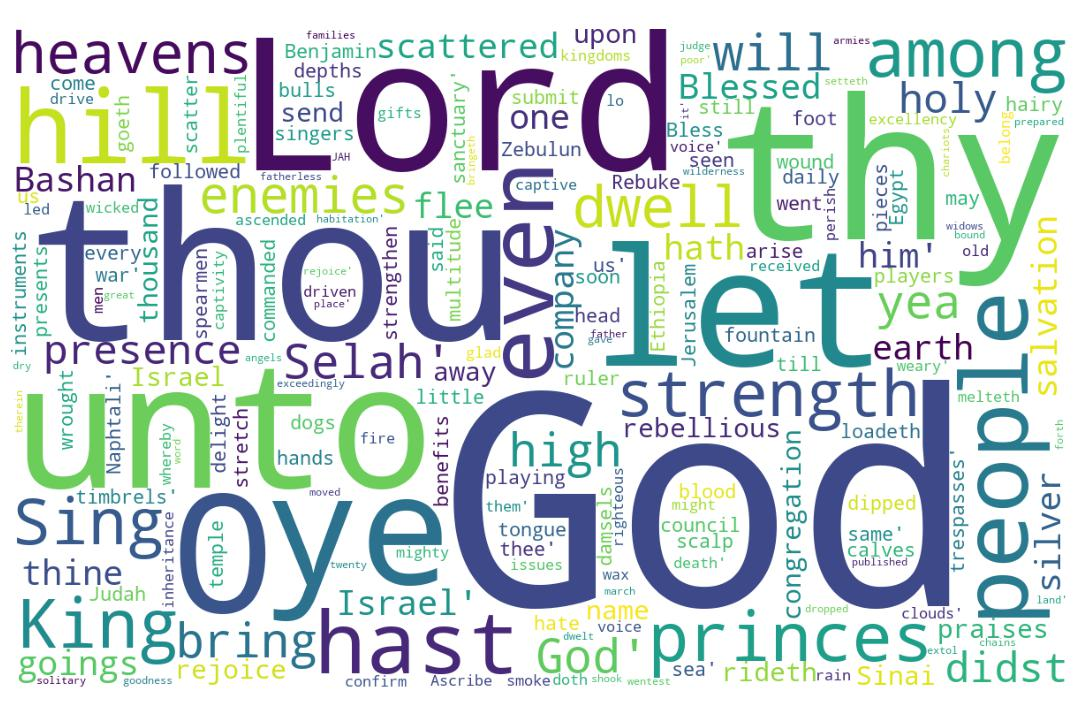
\includegraphics[width=\linewidth]{19OT-Psalms/Psalm68-WordCloud.jpg}
  \caption{Psalm 68 Word Cloud}
  \label{fig:Psalm 68 word Cloud}
\end{figure}

\marginpar{\scriptsize \centering \fcolorbox{bone}{lime}{\textbf{THINGS THAT BELONG TO GOD}}\\ (Psalm 68:1-35) \begin{compactenum}[I.][8]
    \item The \textbf{Removal} of his Enemies \index[scripture]{Psalms!Psa 068:02}(Psa 68:2)
    \item \textbf{Ministry}  \index[scripture]{Psalms!Psa 068:11}(Psa 68:11)
    \begin{compactenum}[A.]
    	\item To Captives \index[scripture]{Psalms!Psa 068:05}(Psa 68:5)
    	\item To Orphans \index[scripture]{Psalms!Psa 068:05}(Psa 68:5)
    	\item To Widows \index[scripture]{Psalms!Psa 068:05}(Psa 68:5)
    	\item To Sinners \index[scripture]{Psalms!Psa 068:20}(Psa 68:20)
    \end{compactenum}
    \item A \textbf{Message}  \index[scripture]{Psalms!Psa 068:11}(Psa 68:11)
    \item \textbf{Men}  \index[scripture]{Psalms!Psa 068:18}(Psa 68:18)
    \item Special \textbf{Music}  \index[scripture]{Psalms!Psa 068:25}(Psa 68:25)
    \item A \textbf{Millennial Reign}  \index[scripture]{Psalms!Psa 068:29}(Psa 68:29)
    \item A \textbf{Might Voice}  \index[scripture]{Psalms!Psa 068:33}(Psa 68:33)
\end{compactenum}}

\footnote{\textcolor[rgb]{0.00,0.25,0.00}{\hyperlink{TOC}{Return to end of Table of Contents.}}}\footnote{\href{https://audiobible.com/bible/psalms_68.html}{\textcolor[cmyk]{0.99998,1,0,0}{Psalm 68 Audio}}}\textcolor[cmyk]{0.99998,1,0,0}{To the chief Musician, A Psalm \emph{or} Song of David.}\\
\\
\textcolor[cmyk]{0.99998,1,0,0}{Let God arise, let his enemies be scattered: let them also that hate him flee before him.}
[2] \textcolor[cmyk]{0.99998,1,0,0}{As smoke is driven away, \emph{so} drive \emph{them} away: as wax melteth before the fire, \emph{so} let the wicked  \fcolorbox{bone}{lime}{perish} at the presence of God.}\footnote{\textbf{Psalm 97:5} - The hills melted like wax at the presence of the LORD, at the presence of the Lord of the whole earth.}\footnote{\textbf{Micah 1:4} - And the mountains shall be molten under him, and the valleys shall be cleft, as wax before the fire, and as the waters that are poured down a steep place.}
[3] \textcolor[cmyk]{0.99998,1,0,0}{But let the righteous be glad; let them rejoice before God: yea, let them exceedingly rejoice.}
[4] \textcolor[cmyk]{0.99998,1,0,0}{Sing unto God, sing praises to his name: extol him that rideth upon the heavens by his name JAH, and rejoice before him.}
[5] \textcolor[cmyk]{0.99998,1,0,0}{A father of the  \fcolorbox{bone}{lime}{fatherless}, and a judge of the  \fcolorbox{bone}{lime}{widows}, \emph{is} God in his holy habitation.}
[6] \textcolor[cmyk]{0.99998,1,0,0}{God setteth the solitary in families: he bringeth out those which are bound with chains: but the rebellious dwell in a dry \emph{land}.}
[7] \textcolor[cmyk]{0.99998,1,0,0}{O God, when thou wentest forth before thy people, when thou didst march through the wilderness; Selah:}
[8] \textcolor[cmyk]{0.99998,1,0,0}{The earth shook, the heavens also dropped at the presence of God: \emph{even} Sinai itself \emph{was} \emph{moved} at the presence of God, the God of Israel.}
[9] \textcolor[cmyk]{0.99998,1,0,0}{Thou, O God, didst send a plentiful rain, whereby thou didst confirm thine inheritance, when it was weary.}
[10] \textcolor[cmyk]{0.99998,1,0,0}{Thy congregation hath dwelt therein: thou, O God, hast prepared of thy goodness for the poor.}
[11] \textcolor[cmyk]{0.99998,1,0,0}{The  \fcolorbox{bone}{lime}{Lord gave the word}: great \emph{was} the company of those that published \emph{it}.}
[12] \textcolor[cmyk]{0.99998,1,0,0}{Kings of armies did flee apace: and she that tarried at home divided the spoil.}
[13] \textcolor[cmyk]{0.99998,1,0,0}{Though ye have lien among the pots, \emph{yet} \emph{shall} \emph{ye} \emph{be} \emph{as} the wings of a dove covered with silver, and her feathers with lime gold.}
[14] \textcolor[cmyk]{0.99998,1,0,0}{When the Almighty scattered kings in it, it was \emph{white} as snow in Salmon.}
[15] \textcolor[cmyk]{0.99998,1,0,0}{The hill of God \emph{is} \emph{as} the hill of Bashan; an high hill \emph{as} the hill of Bashan.}
[16] \textcolor[cmyk]{0.99998,1,0,0}{Why leap ye, ye high hills? \emph{this} \emph{is} the hill \emph{which} God desireth to dwell in; yea, the LORD will dwell \emph{in} \emph{it} for ever.}
[17] \textcolor[cmyk]{0.99998,1,0,0}{The chariots of God \emph{are} twenty thousand, \emph{even} thousands of angels: the Lord \emph{is} among them, \emph{as} \emph{in} Sinai, in the holy \emph{place}.}
[18] \textcolor[cmyk]{0.99998,1,0,0}{Thou hast ascended on high, thou hast led captivity captive: thou hast received  \fcolorbox{bone}{lime}{gifts for men}; yea, \emph{for} the rebellious also, that the LORD God might dwell \emph{among} \emph{them}.}
[19] \textcolor[cmyk]{0.99998,1,0,0}{Blessed \emph{be} the Lord, \emph{who} daily loadeth us \emph{with} \emph{benefits,} \emph{even} the God of our salvation. Selah.}
[20] \textcolor[cmyk]{0.99998,1,0,0}{\emph{He} \emph{that} \emph{is} our God \emph{is} the God of  \fcolorbox{bone}{lime}{salvation}; and unto GOD the Lord \emph{belong} the issues from death.}
[21] \textcolor[cmyk]{0.99998,1,0,0}{But God shall wound the head of his enemies, \emph{and} the hairy scalp of such an one as goeth on still in his trespasses.}
[22] \textcolor[cmyk]{0.99998,1,0,0}{The Lord said, I will bring again from Bashan, I will bring \emph{my} \emph{people} again from the depths of the sea:}
[23] \textcolor[cmyk]{0.99998,1,0,0}{That thy foot may be dipped in the blood of \emph{thine} enemies, \emph{and} the tongue of thy dogs in the same.}
[24] \textcolor[cmyk]{0.99998,1,0,0}{They have seen thy goings, O God; \emph{even} the goings of my God, my King, in the sanctuary.}
[25] \textcolor[cmyk]{0.99998,1,0,0}{The  \fcolorbox{bone}{lime}{singers} went before, the players on  \fcolorbox{bone}{lime}{instruments} \emph{followed} after; among \emph{them} \emph{were} the damsels playing with  \fcolorbox{bone}{lime}{timbrels}.}
[26] \textcolor[cmyk]{0.99998,1,0,0}{Bless ye God in the \fcolorbox{bone}{MYGOLD}{congregations}, \emph{even} the Lord, from the fountain of Israel.}
[27] \textcolor[cmyk]{0.99998,1,0,0}{There \emph{is} little Benjamin \emph{with} their ruler, the princes of Judah \emph{and} their council, the princes of Zebulun, \emph{and} the princes of Naphtali.}
[28] \textcolor[cmyk]{0.99998,1,0,0}{Thy God hath commanded thy strength: strengthen, O God, that which thou hast wrought for us.}
[29] \textcolor[cmyk]{0.99998,1,0,0}{Because of thy  \fcolorbox{bone}{lime}{temple} at Jerusalem shall kings bring presents unto thee.}
[30] \textcolor[cmyk]{0.99998,1,0,0}{Rebuke the company of spearmen, the multitude of the bulls, with the calves of the people, \emph{till} \emph{every} \emph{one} submit himself with pieces of silver: scatter thou the people \emph{that} delight in war.}
[31] \textcolor[cmyk]{0.99998,1,0,0}{Princes shall come out of Egypt; Ethiopia shall soon stretch out her hands unto God.}
[32] \textcolor[cmyk]{0.99998,1,0,0}{Sing unto God, ye kingdoms of the earth; O sing praises unto the Lord; Selah:}
[33] \textcolor[cmyk]{0.99998,1,0,0}{To him that rideth upon the heavens of heavens, \emph{which} \emph{were} of old; lo, he doth send out his  \fcolorbox{bone}{lime}{voice}, \emph{and} \emph{that} a mighty  \fcolorbox{bone}{lime}{voice}.}
[34] \textcolor[cmyk]{0.99998,1,0,0}{Ascribe ye strength unto God: his excellency \emph{is} over Israel, and his strength \emph{is} in the clouds.}
[35] \textcolor[cmyk]{0.99998,1,0,0}{O God, \emph{thou} \emph{art} terrible out of thy holy places: the God of Israel \emph{is} he that giveth strength and power unto \emph{his} people. Blessed \emph{be} God.}
\index[NWIV]{17!Psalms!Psa 68:1}\index[AWIP]{Let!Psalms!Psa 68:1}\index[AWIP]{God!Psalms!Psa 68:1}\index[AWIP]{arise!Psalms!Psa 68:1}\index[AWIP]{let!Psalms!Psa 68:1}\index[AWIP]{let!Psalms!Psa 68:1 (2)}\index[AWIP]{his!Psalms!Psa 68:1}\index[AWIP]{enemies!Psalms!Psa 68:1}\index[AWIP]{be!Psalms!Psa 68:1}\index[AWIP]{scattered!Psalms!Psa 68:1}\index[AWIP]{them!Psalms!Psa 68:1}\index[AWIP]{also!Psalms!Psa 68:1}\index[AWIP]{that!Psalms!Psa 68:1}\index[AWIP]{hate!Psalms!Psa 68:1}\index[AWIP]{him!Psalms!Psa 68:1}\index[AWIP]{him!Psalms!Psa 68:1 (2)}\index[AWIP]{flee!Psalms!Psa 68:1}\index[AWIP]{before!Psalms!Psa 68:1}

\index[NWIV]{25!Psalms!Psa 68:2}\index[AWIP]{As!Psalms!Psa 68:2}\index[AWIP]{smoke!Psalms!Psa 68:2}\index[AWIP]{is!Psalms!Psa 68:2}\index[AWIP]{driven!Psalms!Psa 68:2}\index[AWIP]{away!Psalms!Psa 68:2}\index[AWIP]{away!Psalms!Psa 68:2 (2)}\index[AWIP]{\emph{so}!Psalms!Psa 68:2}\index[AWIP]{\emph{so}!Psalms!Psa 68:2 (2)}\index[AWIP]{drive!Psalms!Psa 68:2}\index[AWIP]{\emph{them}!Psalms!Psa 68:2}\index[AWIP]{as!Psalms!Psa 68:2}\index[AWIP]{wax!Psalms!Psa 68:2}\index[AWIP]{melteth!Psalms!Psa 68:2}\index[AWIP]{before!Psalms!Psa 68:2}\index[AWIP]{the!Psalms!Psa 68:2}\index[AWIP]{the!Psalms!Psa 68:2 (2)}\index[AWIP]{the!Psalms!Psa 68:2 (3)}\index[AWIP]{fire!Psalms!Psa 68:2}\index[AWIP]{let!Psalms!Psa 68:2}\index[AWIP]{wicked!Psalms!Psa 68:2}\index[AWIP]{perish!Psalms!Psa 68:2}\index[AWIP]{at!Psalms!Psa 68:2}\index[AWIP]{presence!Psalms!Psa 68:2}\index[AWIP]{of!Psalms!Psa 68:2}\index[AWIP]{God!Psalms!Psa 68:2}\index[AWIP]{\emph{so}!Psalms!Psa 68:2}\index[AWIP]{\emph{so}!Psalms!Psa 68:2 (2)}\index[AWIP]{\emph{them}!Psalms!Psa 68:2}

\index[NWIV]{16!Psalms!Psa 68:3}\index[AWIP]{But!Psalms!Psa 68:3}\index[AWIP]{let!Psalms!Psa 68:3}\index[AWIP]{let!Psalms!Psa 68:3 (2)}\index[AWIP]{let!Psalms!Psa 68:3 (3)}\index[AWIP]{the!Psalms!Psa 68:3}\index[AWIP]{righteous!Psalms!Psa 68:3}\index[AWIP]{be!Psalms!Psa 68:3}\index[AWIP]{glad!Psalms!Psa 68:3}\index[AWIP]{them!Psalms!Psa 68:3}\index[AWIP]{them!Psalms!Psa 68:3 (2)}\index[AWIP]{rejoice!Psalms!Psa 68:3}\index[AWIP]{rejoice!Psalms!Psa 68:3 (2)}\index[AWIP]{before!Psalms!Psa 68:3}\index[AWIP]{God!Psalms!Psa 68:3}\index[AWIP]{yea!Psalms!Psa 68:3}\index[AWIP]{exceedingly!Psalms!Psa 68:3}

\index[NWIV]{23!Psalms!Psa 68:4}\index[AWIP]{Sing!Psalms!Psa 68:4}\index[AWIP]{unto!Psalms!Psa 68:4}\index[AWIP]{God!Psalms!Psa 68:4}\index[AWIP]{sing!Psalms!Psa 68:4}\index[AWIP]{praises!Psalms!Psa 68:4}\index[AWIP]{to!Psalms!Psa 68:4}\index[AWIP]{his!Psalms!Psa 68:4}\index[AWIP]{his!Psalms!Psa 68:4 (2)}\index[AWIP]{name!Psalms!Psa 68:4}\index[AWIP]{name!Psalms!Psa 68:4 (2)}\index[AWIP]{extol!Psalms!Psa 68:4}\index[AWIP]{him!Psalms!Psa 68:4}\index[AWIP]{him!Psalms!Psa 68:4 (2)}\index[AWIP]{that!Psalms!Psa 68:4}\index[AWIP]{rideth!Psalms!Psa 68:4}\index[AWIP]{upon!Psalms!Psa 68:4}\index[AWIP]{the!Psalms!Psa 68:4}\index[AWIP]{heavens!Psalms!Psa 68:4}\index[AWIP]{by!Psalms!Psa 68:4}\index[AWIP]{JAH!Psalms!Psa 68:4}\index[AWIP]{and!Psalms!Psa 68:4}\index[AWIP]{rejoice!Psalms!Psa 68:4}\index[AWIP]{before!Psalms!Psa 68:4}

\index[NWIV]{17!Psalms!Psa 68:5}\index[AWIP]{A!Psalms!Psa 68:5}\index[AWIP]{father!Psalms!Psa 68:5}\index[AWIP]{of!Psalms!Psa 68:5}\index[AWIP]{of!Psalms!Psa 68:5 (2)}\index[AWIP]{the!Psalms!Psa 68:5}\index[AWIP]{the!Psalms!Psa 68:5 (2)}\index[AWIP]{fatherless!Psalms!Psa 68:5}\index[AWIP]{and!Psalms!Psa 68:5}\index[AWIP]{a!Psalms!Psa 68:5}\index[AWIP]{judge!Psalms!Psa 68:5}\index[AWIP]{widows!Psalms!Psa 68:5}\index[AWIP]{\emph{is}!Psalms!Psa 68:5}\index[AWIP]{God!Psalms!Psa 68:5}\index[AWIP]{in!Psalms!Psa 68:5}\index[AWIP]{his!Psalms!Psa 68:5}\index[AWIP]{holy!Psalms!Psa 68:5}\index[AWIP]{habitation!Psalms!Psa 68:5}\index[AWIP]{\emph{is}!Psalms!Psa 68:5}

\index[NWIV]{23!Psalms!Psa 68:6}\index[AWIP]{God!Psalms!Psa 68:6}\index[AWIP]{setteth!Psalms!Psa 68:6}\index[AWIP]{the!Psalms!Psa 68:6}\index[AWIP]{the!Psalms!Psa 68:6 (2)}\index[AWIP]{solitary!Psalms!Psa 68:6}\index[AWIP]{in!Psalms!Psa 68:6}\index[AWIP]{in!Psalms!Psa 68:6 (2)}\index[AWIP]{families!Psalms!Psa 68:6}\index[AWIP]{he!Psalms!Psa 68:6}\index[AWIP]{bringeth!Psalms!Psa 68:6}\index[AWIP]{out!Psalms!Psa 68:6}\index[AWIP]{those!Psalms!Psa 68:6}\index[AWIP]{which!Psalms!Psa 68:6}\index[AWIP]{are!Psalms!Psa 68:6}\index[AWIP]{bound!Psalms!Psa 68:6}\index[AWIP]{with!Psalms!Psa 68:6}\index[AWIP]{chains!Psalms!Psa 68:6}\index[AWIP]{but!Psalms!Psa 68:6}\index[AWIP]{rebellious!Psalms!Psa 68:6}\index[AWIP]{dwell!Psalms!Psa 68:6}\index[AWIP]{a!Psalms!Psa 68:6}\index[AWIP]{dry!Psalms!Psa 68:6}\index[AWIP]{\emph{land}!Psalms!Psa 68:6}\index[AWIP]{\emph{land}!Psalms!Psa 68:6}

\index[NWIV]{17!Psalms!Psa 68:7}\index[AWIP]{O!Psalms!Psa 68:7}\index[AWIP]{God!Psalms!Psa 68:7}\index[AWIP]{when!Psalms!Psa 68:7}\index[AWIP]{when!Psalms!Psa 68:7 (2)}\index[AWIP]{thou!Psalms!Psa 68:7}\index[AWIP]{thou!Psalms!Psa 68:7 (2)}\index[AWIP]{wentest!Psalms!Psa 68:7}\index[AWIP]{forth!Psalms!Psa 68:7}\index[AWIP]{before!Psalms!Psa 68:7}\index[AWIP]{thy!Psalms!Psa 68:7}\index[AWIP]{people!Psalms!Psa 68:7}\index[AWIP]{didst!Psalms!Psa 68:7}\index[AWIP]{march!Psalms!Psa 68:7}\index[AWIP]{through!Psalms!Psa 68:7}\index[AWIP]{the!Psalms!Psa 68:7}\index[AWIP]{wilderness!Psalms!Psa 68:7}\index[AWIP]{Selah!Psalms!Psa 68:7}

\index[NWIV]{26!Psalms!Psa 68:8}\index[AWIP]{The!Psalms!Psa 68:8}\index[AWIP]{earth!Psalms!Psa 68:8}\index[AWIP]{shook!Psalms!Psa 68:8}\index[AWIP]{the!Psalms!Psa 68:8}\index[AWIP]{the!Psalms!Psa 68:8 (2)}\index[AWIP]{the!Psalms!Psa 68:8 (3)}\index[AWIP]{the!Psalms!Psa 68:8 (4)}\index[AWIP]{heavens!Psalms!Psa 68:8}\index[AWIP]{also!Psalms!Psa 68:8}\index[AWIP]{dropped!Psalms!Psa 68:8}\index[AWIP]{at!Psalms!Psa 68:8}\index[AWIP]{at!Psalms!Psa 68:8 (2)}\index[AWIP]{presence!Psalms!Psa 68:8}\index[AWIP]{presence!Psalms!Psa 68:8 (2)}\index[AWIP]{of!Psalms!Psa 68:8}\index[AWIP]{of!Psalms!Psa 68:8 (2)}\index[AWIP]{of!Psalms!Psa 68:8 (3)}\index[AWIP]{God!Psalms!Psa 68:8}\index[AWIP]{God!Psalms!Psa 68:8 (2)}\index[AWIP]{God!Psalms!Psa 68:8 (3)}\index[AWIP]{\emph{even}!Psalms!Psa 68:8}\index[AWIP]{Sinai!Psalms!Psa 68:8}\index[AWIP]{itself!Psalms!Psa 68:8}\index[AWIP]{\emph{was}!Psalms!Psa 68:8}\index[AWIP]{\emph{moved}!Psalms!Psa 68:8}\index[AWIP]{Israel!Psalms!Psa 68:8}\index[AWIP]{\emph{even}!Psalms!Psa 68:8}\index[AWIP]{\emph{was}!Psalms!Psa 68:8}\index[AWIP]{\emph{moved}!Psalms!Psa 68:8}

\index[NWIV]{18!Psalms!Psa 68:9}\index[AWIP]{Thou!Psalms!Psa 68:9}\index[AWIP]{O!Psalms!Psa 68:9}\index[AWIP]{God!Psalms!Psa 68:9}\index[AWIP]{didst!Psalms!Psa 68:9}\index[AWIP]{didst!Psalms!Psa 68:9 (2)}\index[AWIP]{send!Psalms!Psa 68:9}\index[AWIP]{a!Psalms!Psa 68:9}\index[AWIP]{plentiful!Psalms!Psa 68:9}\index[AWIP]{rain!Psalms!Psa 68:9}\index[AWIP]{whereby!Psalms!Psa 68:9}\index[AWIP]{thou!Psalms!Psa 68:9}\index[AWIP]{confirm!Psalms!Psa 68:9}\index[AWIP]{thine!Psalms!Psa 68:9}\index[AWIP]{inheritance!Psalms!Psa 68:9}\index[AWIP]{when!Psalms!Psa 68:9}\index[AWIP]{it!Psalms!Psa 68:9}\index[AWIP]{was!Psalms!Psa 68:9}\index[AWIP]{weary!Psalms!Psa 68:9}

\index[NWIV]{16!Psalms!Psa 68:10}\index[AWIP]{Thy!Psalms!Psa 68:10}\index[AWIP]{congregation!Psalms!Psa 68:10}\index[AWIP]{hath!Psalms!Psa 68:10}\index[AWIP]{dwelt!Psalms!Psa 68:10}\index[AWIP]{therein!Psalms!Psa 68:10}\index[AWIP]{thou!Psalms!Psa 68:10}\index[AWIP]{O!Psalms!Psa 68:10}\index[AWIP]{God!Psalms!Psa 68:10}\index[AWIP]{hast!Psalms!Psa 68:10}\index[AWIP]{prepared!Psalms!Psa 68:10}\index[AWIP]{of!Psalms!Psa 68:10}\index[AWIP]{thy!Psalms!Psa 68:10}\index[AWIP]{goodness!Psalms!Psa 68:10}\index[AWIP]{for!Psalms!Psa 68:10}\index[AWIP]{the!Psalms!Psa 68:10}\index[AWIP]{poor!Psalms!Psa 68:10}

\index[NWIV]{14!Psalms!Psa 68:11}\index[AWIP]{The!Psalms!Psa 68:11}\index[AWIP]{Lord!Psalms!Psa 68:11}\index[AWIP]{gave!Psalms!Psa 68:11}\index[AWIP]{the!Psalms!Psa 68:11}\index[AWIP]{the!Psalms!Psa 68:11 (2)}\index[AWIP]{word!Psalms!Psa 68:11}\index[AWIP]{great!Psalms!Psa 68:11}\index[AWIP]{\emph{was}!Psalms!Psa 68:11}\index[AWIP]{company!Psalms!Psa 68:11}\index[AWIP]{of!Psalms!Psa 68:11}\index[AWIP]{those!Psalms!Psa 68:11}\index[AWIP]{that!Psalms!Psa 68:11}\index[AWIP]{published!Psalms!Psa 68:11}\index[AWIP]{\emph{it}!Psalms!Psa 68:11}\index[AWIP]{\emph{was}!Psalms!Psa 68:11}\index[AWIP]{\emph{it}!Psalms!Psa 68:11}

\index[NWIV]{15!Psalms!Psa 68:12}\index[AWIP]{Kings!Psalms!Psa 68:12}\index[AWIP]{of!Psalms!Psa 68:12}\index[AWIP]{armies!Psalms!Psa 68:12}\index[AWIP]{did!Psalms!Psa 68:12}\index[AWIP]{flee!Psalms!Psa 68:12}\index[AWIP]{apace!Psalms!Psa 68:12}\index[AWIP]{and!Psalms!Psa 68:12}\index[AWIP]{she!Psalms!Psa 68:12}\index[AWIP]{that!Psalms!Psa 68:12}\index[AWIP]{tarried!Psalms!Psa 68:12}\index[AWIP]{at!Psalms!Psa 68:12}\index[AWIP]{home!Psalms!Psa 68:12}\index[AWIP]{divided!Psalms!Psa 68:12}\index[AWIP]{the!Psalms!Psa 68:12}\index[AWIP]{spoil!Psalms!Psa 68:12}

\index[NWIV]{26!Psalms!Psa 68:13}\index[AWIP]{Though!Psalms!Psa 68:13}\index[AWIP]{ye!Psalms!Psa 68:13}\index[AWIP]{have!Psalms!Psa 68:13}\index[AWIP]{lien!Psalms!Psa 68:13}\index[AWIP]{among!Psalms!Psa 68:13}\index[AWIP]{the!Psalms!Psa 68:13}\index[AWIP]{the!Psalms!Psa 68:13 (2)}\index[AWIP]{pots!Psalms!Psa 68:13}\index[AWIP]{\emph{yet}!Psalms!Psa 68:13}\index[AWIP]{\emph{shall}!Psalms!Psa 68:13}\index[AWIP]{\emph{ye}!Psalms!Psa 68:13}\index[AWIP]{\emph{be}!Psalms!Psa 68:13}\index[AWIP]{\emph{as}!Psalms!Psa 68:13}\index[AWIP]{wings!Psalms!Psa 68:13}\index[AWIP]{of!Psalms!Psa 68:13}\index[AWIP]{a!Psalms!Psa 68:13}\index[AWIP]{dove!Psalms!Psa 68:13}\index[AWIP]{covered!Psalms!Psa 68:13}\index[AWIP]{with!Psalms!Psa 68:13}\index[AWIP]{with!Psalms!Psa 68:13 (2)}\index[AWIP]{silver!Psalms!Psa 68:13}\index[AWIP]{and!Psalms!Psa 68:13}\index[AWIP]{her!Psalms!Psa 68:13}\index[AWIP]{feathers!Psalms!Psa 68:13}\index[AWIP]{yellow!Psalms!Psa 68:13}\index[AWIP]{gold!Psalms!Psa 68:13}\index[AWIP]{\emph{yet}!Psalms!Psa 68:13}\index[AWIP]{\emph{shall}!Psalms!Psa 68:13}\index[AWIP]{\emph{ye}!Psalms!Psa 68:13}\index[AWIP]{\emph{be}!Psalms!Psa 68:13}\index[AWIP]{\emph{as}!Psalms!Psa 68:13}

\index[NWIV]{14!Psalms!Psa 68:14}\index[AWIP]{When!Psalms!Psa 68:14}\index[AWIP]{the!Psalms!Psa 68:14}\index[AWIP]{Almighty!Psalms!Psa 68:14}\index[AWIP]{scattered!Psalms!Psa 68:14}\index[AWIP]{kings!Psalms!Psa 68:14}\index[AWIP]{in!Psalms!Psa 68:14}\index[AWIP]{in!Psalms!Psa 68:14 (2)}\index[AWIP]{it!Psalms!Psa 68:14}\index[AWIP]{it!Psalms!Psa 68:14 (2)}\index[AWIP]{was!Psalms!Psa 68:14}\index[AWIP]{\emph{white}!Psalms!Psa 68:14}\index[AWIP]{as!Psalms!Psa 68:14}\index[AWIP]{snow!Psalms!Psa 68:14}\index[AWIP]{Salmon!Psalms!Psa 68:14}\index[AWIP]{\emph{white}!Psalms!Psa 68:14}

\index[NWIV]{18!Psalms!Psa 68:15}\index[AWIP]{The!Psalms!Psa 68:15}\index[AWIP]{hill!Psalms!Psa 68:15}\index[AWIP]{hill!Psalms!Psa 68:15 (2)}\index[AWIP]{hill!Psalms!Psa 68:15 (3)}\index[AWIP]{hill!Psalms!Psa 68:15 (4)}\index[AWIP]{of!Psalms!Psa 68:15}\index[AWIP]{of!Psalms!Psa 68:15 (2)}\index[AWIP]{of!Psalms!Psa 68:15 (3)}\index[AWIP]{God!Psalms!Psa 68:15}\index[AWIP]{\emph{is}!Psalms!Psa 68:15}\index[AWIP]{\emph{as}!Psalms!Psa 68:15}\index[AWIP]{\emph{as}!Psalms!Psa 68:15 (2)}\index[AWIP]{the!Psalms!Psa 68:15}\index[AWIP]{the!Psalms!Psa 68:15 (2)}\index[AWIP]{Bashan!Psalms!Psa 68:15}\index[AWIP]{Bashan!Psalms!Psa 68:15 (2)}\index[AWIP]{an!Psalms!Psa 68:15}\index[AWIP]{high!Psalms!Psa 68:15}\index[AWIP]{\emph{is}!Psalms!Psa 68:15}\index[AWIP]{\emph{as}!Psalms!Psa 68:15}\index[AWIP]{\emph{as}!Psalms!Psa 68:15 (2)}

\index[NWIV]{25!Psalms!Psa 68:16}\index[AWIP]{Why!Psalms!Psa 68:16}\index[AWIP]{leap!Psalms!Psa 68:16}\index[AWIP]{ye!Psalms!Psa 68:16}\index[AWIP]{ye!Psalms!Psa 68:16 (2)}\index[AWIP]{high!Psalms!Psa 68:16}\index[AWIP]{hills?!Psalms!Psa 68:16}\index[AWIP]{\emph{this}!Psalms!Psa 68:16}\index[AWIP]{\emph{is}!Psalms!Psa 68:16}\index[AWIP]{the!Psalms!Psa 68:16}\index[AWIP]{the!Psalms!Psa 68:16 (2)}\index[AWIP]{hill!Psalms!Psa 68:16}\index[AWIP]{\emph{which}!Psalms!Psa 68:16}\index[AWIP]{God!Psalms!Psa 68:16}\index[AWIP]{desireth!Psalms!Psa 68:16}\index[AWIP]{to!Psalms!Psa 68:16}\index[AWIP]{dwell!Psalms!Psa 68:16}\index[AWIP]{dwell!Psalms!Psa 68:16 (2)}\index[AWIP]{in!Psalms!Psa 68:16}\index[AWIP]{yea!Psalms!Psa 68:16}\index[AWIP]{LORD!Psalms!Psa 68:16}\index[AWIP]{will!Psalms!Psa 68:16}\index[AWIP]{\emph{in}!Psalms!Psa 68:16}\index[AWIP]{\emph{it}!Psalms!Psa 68:16}\index[AWIP]{for!Psalms!Psa 68:16}\index[AWIP]{ever!Psalms!Psa 68:16}\index[AWIP]{\emph{this}!Psalms!Psa 68:16}\index[AWIP]{\emph{is}!Psalms!Psa 68:16}\index[AWIP]{\emph{which}!Psalms!Psa 68:16}\index[AWIP]{\emph{in}!Psalms!Psa 68:16}\index[AWIP]{\emph{it}!Psalms!Psa 68:16}

\index[NWIV]{23!Psalms!Psa 68:17}\index[AWIP]{The!Psalms!Psa 68:17}\index[AWIP]{chariots!Psalms!Psa 68:17}\index[AWIP]{of!Psalms!Psa 68:17}\index[AWIP]{of!Psalms!Psa 68:17 (2)}\index[AWIP]{God!Psalms!Psa 68:17}\index[AWIP]{\emph{are}!Psalms!Psa 68:17}\index[AWIP]{twenty!Psalms!Psa 68:17}\index[AWIP]{thousand!Psalms!Psa 68:17}\index[AWIP]{\emph{even}!Psalms!Psa 68:17}\index[AWIP]{thousands!Psalms!Psa 68:17}\index[AWIP]{angels!Psalms!Psa 68:17}\index[AWIP]{the!Psalms!Psa 68:17}\index[AWIP]{the!Psalms!Psa 68:17 (2)}\index[AWIP]{Lord!Psalms!Psa 68:17}\index[AWIP]{\emph{is}!Psalms!Psa 68:17}\index[AWIP]{among!Psalms!Psa 68:17}\index[AWIP]{them!Psalms!Psa 68:17}\index[AWIP]{\emph{as}!Psalms!Psa 68:17}\index[AWIP]{\emph{in}!Psalms!Psa 68:17}\index[AWIP]{Sinai!Psalms!Psa 68:17}\index[AWIP]{in!Psalms!Psa 68:17}\index[AWIP]{holy!Psalms!Psa 68:17}\index[AWIP]{\emph{place}!Psalms!Psa 68:17}\index[AWIP]{\emph{are}!Psalms!Psa 68:17}\index[AWIP]{\emph{even}!Psalms!Psa 68:17}\index[AWIP]{\emph{is}!Psalms!Psa 68:17}\index[AWIP]{\emph{as}!Psalms!Psa 68:17}\index[AWIP]{\emph{in}!Psalms!Psa 68:17}\index[AWIP]{\emph{place}!Psalms!Psa 68:17}

\index[NWIV]{29!Psalms!Psa 68:18}\index[AWIP]{Thou!Psalms!Psa 68:18}\index[AWIP]{hast!Psalms!Psa 68:18}\index[AWIP]{hast!Psalms!Psa 68:18 (2)}\index[AWIP]{hast!Psalms!Psa 68:18 (3)}\index[AWIP]{ascended!Psalms!Psa 68:18}\index[AWIP]{on!Psalms!Psa 68:18}\index[AWIP]{high!Psalms!Psa 68:18}\index[AWIP]{thou!Psalms!Psa 68:18}\index[AWIP]{thou!Psalms!Psa 68:18 (2)}\index[AWIP]{led!Psalms!Psa 68:18}\index[AWIP]{captivity!Psalms!Psa 68:18}\index[AWIP]{captive!Psalms!Psa 68:18}\index[AWIP]{received!Psalms!Psa 68:18}\index[AWIP]{gifts!Psalms!Psa 68:18}\index[AWIP]{for!Psalms!Psa 68:18}\index[AWIP]{men!Psalms!Psa 68:18}\index[AWIP]{yea!Psalms!Psa 68:18}\index[AWIP]{\emph{for}!Psalms!Psa 68:18}\index[AWIP]{the!Psalms!Psa 68:18}\index[AWIP]{the!Psalms!Psa 68:18 (2)}\index[AWIP]{rebellious!Psalms!Psa 68:18}\index[AWIP]{also!Psalms!Psa 68:18}\index[AWIP]{that!Psalms!Psa 68:18}\index[AWIP]{LORD!Psalms!Psa 68:18}\index[AWIP]{God!Psalms!Psa 68:18}\index[AWIP]{might!Psalms!Psa 68:18}\index[AWIP]{dwell!Psalms!Psa 68:18}\index[AWIP]{\emph{among}!Psalms!Psa 68:18}\index[AWIP]{\emph{them}!Psalms!Psa 68:18}\index[AWIP]{\emph{for}!Psalms!Psa 68:18}\index[AWIP]{\emph{among}!Psalms!Psa 68:18}\index[AWIP]{\emph{them}!Psalms!Psa 68:18}

\index[NWIV]{17!Psalms!Psa 68:19}\index[AWIP]{Blessed!Psalms!Psa 68:19}\index[AWIP]{\emph{be}!Psalms!Psa 68:19}\index[AWIP]{the!Psalms!Psa 68:19}\index[AWIP]{the!Psalms!Psa 68:19 (2)}\index[AWIP]{Lord!Psalms!Psa 68:19}\index[AWIP]{\emph{who}!Psalms!Psa 68:19}\index[AWIP]{daily!Psalms!Psa 68:19}\index[AWIP]{loadeth!Psalms!Psa 68:19}\index[AWIP]{us!Psalms!Psa 68:19}\index[AWIP]{\emph{with}!Psalms!Psa 68:19}\index[AWIP]{\emph{benefits}!Psalms!Psa 68:19}\index[AWIP]{\emph{even}!Psalms!Psa 68:19}\index[AWIP]{God!Psalms!Psa 68:19}\index[AWIP]{of!Psalms!Psa 68:19}\index[AWIP]{our!Psalms!Psa 68:19}\index[AWIP]{salvation!Psalms!Psa 68:19}\index[AWIP]{Selah!Psalms!Psa 68:19}\index[AWIP]{\emph{be}!Psalms!Psa 68:19}\index[AWIP]{\emph{who}!Psalms!Psa 68:19}\index[AWIP]{\emph{with}!Psalms!Psa 68:19}\index[AWIP]{\emph{benefits}!Psalms!Psa 68:19}\index[AWIP]{\emph{even}!Psalms!Psa 68:19}

\index[NWIV]{20!Psalms!Psa 68:20}\index[AWIP]{\emph{He}!Psalms!Psa 68:20}\index[AWIP]{\emph{that}!Psalms!Psa 68:20}\index[AWIP]{\emph{is}!Psalms!Psa 68:20}\index[AWIP]{\emph{is}!Psalms!Psa 68:20 (2)}\index[AWIP]{our!Psalms!Psa 68:20}\index[AWIP]{God!Psalms!Psa 68:20}\index[AWIP]{God!Psalms!Psa 68:20 (2)}\index[AWIP]{the!Psalms!Psa 68:20}\index[AWIP]{the!Psalms!Psa 68:20 (2)}\index[AWIP]{the!Psalms!Psa 68:20 (3)}\index[AWIP]{of!Psalms!Psa 68:20}\index[AWIP]{salvation!Psalms!Psa 68:20}\index[AWIP]{and!Psalms!Psa 68:20}\index[AWIP]{unto!Psalms!Psa 68:20}\index[AWIP]{GOD!Psalms!Psa 68:20}\index[AWIP]{Lord!Psalms!Psa 68:20}\index[AWIP]{\emph{belong}!Psalms!Psa 68:20}\index[AWIP]{issues!Psalms!Psa 68:20}\index[AWIP]{from!Psalms!Psa 68:20}\index[AWIP]{death!Psalms!Psa 68:20}\index[AWIP]{\emph{He}!Psalms!Psa 68:20}\index[AWIP]{\emph{that}!Psalms!Psa 68:20}\index[AWIP]{\emph{is}!Psalms!Psa 68:20}\index[AWIP]{\emph{is}!Psalms!Psa 68:20 (2)}\index[AWIP]{\emph{belong}!Psalms!Psa 68:20}

\index[NWIV]{24!Psalms!Psa 68:21}\index[AWIP]{But!Psalms!Psa 68:21}\index[AWIP]{God!Psalms!Psa 68:21}\index[AWIP]{shall!Psalms!Psa 68:21}\index[AWIP]{wound!Psalms!Psa 68:21}\index[AWIP]{the!Psalms!Psa 68:21}\index[AWIP]{the!Psalms!Psa 68:21 (2)}\index[AWIP]{head!Psalms!Psa 68:21}\index[AWIP]{of!Psalms!Psa 68:21}\index[AWIP]{of!Psalms!Psa 68:21 (2)}\index[AWIP]{his!Psalms!Psa 68:21}\index[AWIP]{his!Psalms!Psa 68:21 (2)}\index[AWIP]{enemies!Psalms!Psa 68:21}\index[AWIP]{\emph{and}!Psalms!Psa 68:21}\index[AWIP]{hairy!Psalms!Psa 68:21}\index[AWIP]{scalp!Psalms!Psa 68:21}\index[AWIP]{such!Psalms!Psa 68:21}\index[AWIP]{an!Psalms!Psa 68:21}\index[AWIP]{one!Psalms!Psa 68:21}\index[AWIP]{as!Psalms!Psa 68:21}\index[AWIP]{goeth!Psalms!Psa 68:21}\index[AWIP]{on!Psalms!Psa 68:21}\index[AWIP]{still!Psalms!Psa 68:21}\index[AWIP]{in!Psalms!Psa 68:21}\index[AWIP]{trespasses!Psalms!Psa 68:21}\index[AWIP]{\emph{and}!Psalms!Psa 68:21}

\index[NWIV]{21!Psalms!Psa 68:22}\index[AWIP]{The!Psalms!Psa 68:22}\index[AWIP]{Lord!Psalms!Psa 68:22}\index[AWIP]{said!Psalms!Psa 68:22}\index[AWIP]{I!Psalms!Psa 68:22}\index[AWIP]{I!Psalms!Psa 68:22 (2)}\index[AWIP]{will!Psalms!Psa 68:22}\index[AWIP]{will!Psalms!Psa 68:22 (2)}\index[AWIP]{bring!Psalms!Psa 68:22}\index[AWIP]{bring!Psalms!Psa 68:22 (2)}\index[AWIP]{again!Psalms!Psa 68:22}\index[AWIP]{again!Psalms!Psa 68:22 (2)}\index[AWIP]{from!Psalms!Psa 68:22}\index[AWIP]{from!Psalms!Psa 68:22 (2)}\index[AWIP]{Bashan!Psalms!Psa 68:22}\index[AWIP]{\emph{my}!Psalms!Psa 68:22}\index[AWIP]{\emph{people}!Psalms!Psa 68:22}\index[AWIP]{the!Psalms!Psa 68:22}\index[AWIP]{the!Psalms!Psa 68:22 (2)}\index[AWIP]{depths!Psalms!Psa 68:22}\index[AWIP]{of!Psalms!Psa 68:22}\index[AWIP]{sea!Psalms!Psa 68:22}\index[AWIP]{\emph{my}!Psalms!Psa 68:22}\index[AWIP]{\emph{people}!Psalms!Psa 68:22}

\index[NWIV]{21!Psalms!Psa 68:23}\index[AWIP]{That!Psalms!Psa 68:23}\index[AWIP]{thy!Psalms!Psa 68:23}\index[AWIP]{thy!Psalms!Psa 68:23 (2)}\index[AWIP]{foot!Psalms!Psa 68:23}\index[AWIP]{may!Psalms!Psa 68:23}\index[AWIP]{be!Psalms!Psa 68:23}\index[AWIP]{dipped!Psalms!Psa 68:23}\index[AWIP]{in!Psalms!Psa 68:23}\index[AWIP]{in!Psalms!Psa 68:23 (2)}\index[AWIP]{the!Psalms!Psa 68:23}\index[AWIP]{the!Psalms!Psa 68:23 (2)}\index[AWIP]{the!Psalms!Psa 68:23 (3)}\index[AWIP]{blood!Psalms!Psa 68:23}\index[AWIP]{of!Psalms!Psa 68:23}\index[AWIP]{of!Psalms!Psa 68:23 (2)}\index[AWIP]{\emph{thine}!Psalms!Psa 68:23}\index[AWIP]{enemies!Psalms!Psa 68:23}\index[AWIP]{\emph{and}!Psalms!Psa 68:23}\index[AWIP]{tongue!Psalms!Psa 68:23}\index[AWIP]{dogs!Psalms!Psa 68:23}\index[AWIP]{same!Psalms!Psa 68:23}\index[AWIP]{\emph{thine}!Psalms!Psa 68:23}\index[AWIP]{\emph{and}!Psalms!Psa 68:23}

\index[NWIV]{18!Psalms!Psa 68:24}\index[AWIP]{They!Psalms!Psa 68:24}\index[AWIP]{have!Psalms!Psa 68:24}\index[AWIP]{seen!Psalms!Psa 68:24}\index[AWIP]{thy!Psalms!Psa 68:24}\index[AWIP]{goings!Psalms!Psa 68:24}\index[AWIP]{goings!Psalms!Psa 68:24 (2)}\index[AWIP]{O!Psalms!Psa 68:24}\index[AWIP]{God!Psalms!Psa 68:24}\index[AWIP]{God!Psalms!Psa 68:24 (2)}\index[AWIP]{\emph{even}!Psalms!Psa 68:24}\index[AWIP]{the!Psalms!Psa 68:24}\index[AWIP]{the!Psalms!Psa 68:24 (2)}\index[AWIP]{of!Psalms!Psa 68:24}\index[AWIP]{my!Psalms!Psa 68:24}\index[AWIP]{my!Psalms!Psa 68:24 (2)}\index[AWIP]{King!Psalms!Psa 68:24}\index[AWIP]{in!Psalms!Psa 68:24}\index[AWIP]{sanctuary!Psalms!Psa 68:24}\index[AWIP]{\emph{even}!Psalms!Psa 68:24}

\index[NWIV]{18!Psalms!Psa 68:25}\index[AWIP]{The!Psalms!Psa 68:25}\index[AWIP]{singers!Psalms!Psa 68:25}\index[AWIP]{went!Psalms!Psa 68:25}\index[AWIP]{before!Psalms!Psa 68:25}\index[AWIP]{the!Psalms!Psa 68:25}\index[AWIP]{the!Psalms!Psa 68:25 (2)}\index[AWIP]{players!Psalms!Psa 68:25}\index[AWIP]{on!Psalms!Psa 68:25}\index[AWIP]{instruments!Psalms!Psa 68:25}\index[AWIP]{\emph{followed}!Psalms!Psa 68:25}\index[AWIP]{after!Psalms!Psa 68:25}\index[AWIP]{among!Psalms!Psa 68:25}\index[AWIP]{\emph{them}!Psalms!Psa 68:25}\index[AWIP]{\emph{were}!Psalms!Psa 68:25}\index[AWIP]{damsels!Psalms!Psa 68:25}\index[AWIP]{playing!Psalms!Psa 68:25}\index[AWIP]{with!Psalms!Psa 68:25}\index[AWIP]{timbrels!Psalms!Psa 68:25}\index[AWIP]{\emph{followed}!Psalms!Psa 68:25}\index[AWIP]{\emph{them}!Psalms!Psa 68:25}\index[AWIP]{\emph{were}!Psalms!Psa 68:25}

\index[NWIV]{14!Psalms!Psa 68:26}\index[AWIP]{Bless!Psalms!Psa 68:26}\index[AWIP]{ye!Psalms!Psa 68:26}\index[AWIP]{God!Psalms!Psa 68:26}\index[AWIP]{in!Psalms!Psa 68:26}\index[AWIP]{the!Psalms!Psa 68:26}\index[AWIP]{the!Psalms!Psa 68:26 (2)}\index[AWIP]{the!Psalms!Psa 68:26 (3)}\index[AWIP]{congregations!Psalms!Psa 68:26}\index[AWIP]{\emph{even}!Psalms!Psa 68:26}\index[AWIP]{Lord!Psalms!Psa 68:26}\index[AWIP]{from!Psalms!Psa 68:26}\index[AWIP]{fountain!Psalms!Psa 68:26}\index[AWIP]{of!Psalms!Psa 68:26}\index[AWIP]{Israel!Psalms!Psa 68:26}\index[AWIP]{\emph{even}!Psalms!Psa 68:26}

\index[NWIV]{23!Psalms!Psa 68:27}\index[AWIP]{There!Psalms!Psa 68:27}\index[AWIP]{\emph{is}!Psalms!Psa 68:27}\index[AWIP]{little!Psalms!Psa 68:27}\index[AWIP]{Benjamin!Psalms!Psa 68:27}\index[AWIP]{\emph{with}!Psalms!Psa 68:27}\index[AWIP]{their!Psalms!Psa 68:27}\index[AWIP]{their!Psalms!Psa 68:27 (2)}\index[AWIP]{ruler!Psalms!Psa 68:27}\index[AWIP]{the!Psalms!Psa 68:27}\index[AWIP]{the!Psalms!Psa 68:27 (2)}\index[AWIP]{the!Psalms!Psa 68:27 (3)}\index[AWIP]{princes!Psalms!Psa 68:27}\index[AWIP]{princes!Psalms!Psa 68:27 (2)}\index[AWIP]{princes!Psalms!Psa 68:27 (3)}\index[AWIP]{of!Psalms!Psa 68:27}\index[AWIP]{of!Psalms!Psa 68:27 (2)}\index[AWIP]{of!Psalms!Psa 68:27 (3)}\index[AWIP]{Judah!Psalms!Psa 68:27}\index[AWIP]{\emph{and}!Psalms!Psa 68:27}\index[AWIP]{\emph{and}!Psalms!Psa 68:27 (2)}\index[AWIP]{council!Psalms!Psa 68:27}\index[AWIP]{Zebulun!Psalms!Psa 68:27}\index[AWIP]{Naphtali!Psalms!Psa 68:27}\index[AWIP]{\emph{is}!Psalms!Psa 68:27}\index[AWIP]{\emph{with}!Psalms!Psa 68:27}\index[AWIP]{\emph{and}!Psalms!Psa 68:27}\index[AWIP]{\emph{and}!Psalms!Psa 68:27 (2)}

\index[NWIV]{16!Psalms!Psa 68:28}\index[AWIP]{Thy!Psalms!Psa 68:28}\index[AWIP]{God!Psalms!Psa 68:28}\index[AWIP]{God!Psalms!Psa 68:28 (2)}\index[AWIP]{hath!Psalms!Psa 68:28}\index[AWIP]{commanded!Psalms!Psa 68:28}\index[AWIP]{thy!Psalms!Psa 68:28}\index[AWIP]{strength!Psalms!Psa 68:28}\index[AWIP]{strengthen!Psalms!Psa 68:28}\index[AWIP]{O!Psalms!Psa 68:28}\index[AWIP]{that!Psalms!Psa 68:28}\index[AWIP]{which!Psalms!Psa 68:28}\index[AWIP]{thou!Psalms!Psa 68:28}\index[AWIP]{hast!Psalms!Psa 68:28}\index[AWIP]{wrought!Psalms!Psa 68:28}\index[AWIP]{for!Psalms!Psa 68:28}\index[AWIP]{us!Psalms!Psa 68:28}

\index[NWIV]{12!Psalms!Psa 68:29}\index[AWIP]{Because!Psalms!Psa 68:29}\index[AWIP]{of!Psalms!Psa 68:29}\index[AWIP]{thy!Psalms!Psa 68:29}\index[AWIP]{temple!Psalms!Psa 68:29}\index[AWIP]{at!Psalms!Psa 68:29}\index[AWIP]{Jerusalem!Psalms!Psa 68:29}\index[AWIP]{shall!Psalms!Psa 68:29}\index[AWIP]{kings!Psalms!Psa 68:29}\index[AWIP]{bring!Psalms!Psa 68:29}\index[AWIP]{presents!Psalms!Psa 68:29}\index[AWIP]{unto!Psalms!Psa 68:29}\index[AWIP]{thee!Psalms!Psa 68:29}

\index[NWIV]{33!Psalms!Psa 68:30}\index[AWIP]{Rebuke!Psalms!Psa 68:30}\index[AWIP]{the!Psalms!Psa 68:30}\index[AWIP]{the!Psalms!Psa 68:30 (2)}\index[AWIP]{the!Psalms!Psa 68:30 (3)}\index[AWIP]{the!Psalms!Psa 68:30 (4)}\index[AWIP]{the!Psalms!Psa 68:30 (5)}\index[AWIP]{the!Psalms!Psa 68:30 (6)}\index[AWIP]{company!Psalms!Psa 68:30}\index[AWIP]{of!Psalms!Psa 68:30}\index[AWIP]{of!Psalms!Psa 68:30 (2)}\index[AWIP]{of!Psalms!Psa 68:30 (3)}\index[AWIP]{of!Psalms!Psa 68:30 (4)}\index[AWIP]{spearmen!Psalms!Psa 68:30}\index[AWIP]{multitude!Psalms!Psa 68:30}\index[AWIP]{bulls!Psalms!Psa 68:30}\index[AWIP]{with!Psalms!Psa 68:30}\index[AWIP]{with!Psalms!Psa 68:30 (2)}\index[AWIP]{calves!Psalms!Psa 68:30}\index[AWIP]{people!Psalms!Psa 68:30}\index[AWIP]{people!Psalms!Psa 68:30 (2)}\index[AWIP]{\emph{till}!Psalms!Psa 68:30}\index[AWIP]{\emph{every}!Psalms!Psa 68:30}\index[AWIP]{\emph{one}!Psalms!Psa 68:30}\index[AWIP]{submit!Psalms!Psa 68:30}\index[AWIP]{himself!Psalms!Psa 68:30}\index[AWIP]{pieces!Psalms!Psa 68:30}\index[AWIP]{silver!Psalms!Psa 68:30}\index[AWIP]{scatter!Psalms!Psa 68:30}\index[AWIP]{thou!Psalms!Psa 68:30}\index[AWIP]{\emph{that}!Psalms!Psa 68:30}\index[AWIP]{delight!Psalms!Psa 68:30}\index[AWIP]{in!Psalms!Psa 68:30}\index[AWIP]{war!Psalms!Psa 68:30}\index[AWIP]{\emph{till}!Psalms!Psa 68:30}\index[AWIP]{\emph{every}!Psalms!Psa 68:30}\index[AWIP]{\emph{one}!Psalms!Psa 68:30}\index[AWIP]{\emph{that}!Psalms!Psa 68:30}

\index[NWIV]{15!Psalms!Psa 68:31}\index[AWIP]{Princes!Psalms!Psa 68:31}\index[AWIP]{shall!Psalms!Psa 68:31}\index[AWIP]{shall!Psalms!Psa 68:31 (2)}\index[AWIP]{come!Psalms!Psa 68:31}\index[AWIP]{out!Psalms!Psa 68:31}\index[AWIP]{out!Psalms!Psa 68:31 (2)}\index[AWIP]{of!Psalms!Psa 68:31}\index[AWIP]{Egypt!Psalms!Psa 68:31}\index[AWIP]{Ethiopia!Psalms!Psa 68:31}\index[AWIP]{soon!Psalms!Psa 68:31}\index[AWIP]{stretch!Psalms!Psa 68:31}\index[AWIP]{her!Psalms!Psa 68:31}\index[AWIP]{hands!Psalms!Psa 68:31}\index[AWIP]{unto!Psalms!Psa 68:31}\index[AWIP]{God!Psalms!Psa 68:31}

\index[NWIV]{15!Psalms!Psa 68:32}\index[AWIP]{Sing!Psalms!Psa 68:32}\index[AWIP]{unto!Psalms!Psa 68:32}\index[AWIP]{unto!Psalms!Psa 68:32 (2)}\index[AWIP]{God!Psalms!Psa 68:32}\index[AWIP]{ye!Psalms!Psa 68:32}\index[AWIP]{kingdoms!Psalms!Psa 68:32}\index[AWIP]{of!Psalms!Psa 68:32}\index[AWIP]{the!Psalms!Psa 68:32}\index[AWIP]{the!Psalms!Psa 68:32 (2)}\index[AWIP]{earth!Psalms!Psa 68:32}\index[AWIP]{O!Psalms!Psa 68:32}\index[AWIP]{sing!Psalms!Psa 68:32}\index[AWIP]{praises!Psalms!Psa 68:32}\index[AWIP]{Lord!Psalms!Psa 68:32}\index[AWIP]{Selah!Psalms!Psa 68:32}

\index[NWIV]{25!Psalms!Psa 68:33}\index[AWIP]{To!Psalms!Psa 68:33}\index[AWIP]{him!Psalms!Psa 68:33}\index[AWIP]{that!Psalms!Psa 68:33}\index[AWIP]{rideth!Psalms!Psa 68:33}\index[AWIP]{upon!Psalms!Psa 68:33}\index[AWIP]{the!Psalms!Psa 68:33}\index[AWIP]{heavens!Psalms!Psa 68:33}\index[AWIP]{heavens!Psalms!Psa 68:33 (2)}\index[AWIP]{of!Psalms!Psa 68:33}\index[AWIP]{of!Psalms!Psa 68:33 (2)}\index[AWIP]{\emph{which}!Psalms!Psa 68:33}\index[AWIP]{\emph{were}!Psalms!Psa 68:33}\index[AWIP]{old!Psalms!Psa 68:33}\index[AWIP]{lo!Psalms!Psa 68:33}\index[AWIP]{he!Psalms!Psa 68:33}\index[AWIP]{doth!Psalms!Psa 68:33}\index[AWIP]{send!Psalms!Psa 68:33}\index[AWIP]{out!Psalms!Psa 68:33}\index[AWIP]{his!Psalms!Psa 68:33}\index[AWIP]{voice!Psalms!Psa 68:33}\index[AWIP]{voice!Psalms!Psa 68:33 (2)}\index[AWIP]{\emph{and}!Psalms!Psa 68:33}\index[AWIP]{\emph{that}!Psalms!Psa 68:33}\index[AWIP]{a!Psalms!Psa 68:33}\index[AWIP]{mighty!Psalms!Psa 68:33}\index[AWIP]{\emph{which}!Psalms!Psa 68:33}\index[AWIP]{\emph{were}!Psalms!Psa 68:33}\index[AWIP]{\emph{and}!Psalms!Psa 68:33}\index[AWIP]{\emph{that}!Psalms!Psa 68:33}

\index[NWIV]{17!Psalms!Psa 68:34}\index[AWIP]{Ascribe!Psalms!Psa 68:34}\index[AWIP]{ye!Psalms!Psa 68:34}\index[AWIP]{strength!Psalms!Psa 68:34}\index[AWIP]{strength!Psalms!Psa 68:34 (2)}\index[AWIP]{unto!Psalms!Psa 68:34}\index[AWIP]{God!Psalms!Psa 68:34}\index[AWIP]{his!Psalms!Psa 68:34}\index[AWIP]{his!Psalms!Psa 68:34 (2)}\index[AWIP]{excellency!Psalms!Psa 68:34}\index[AWIP]{\emph{is}!Psalms!Psa 68:34}\index[AWIP]{\emph{is}!Psalms!Psa 68:34 (2)}\index[AWIP]{over!Psalms!Psa 68:34}\index[AWIP]{Israel!Psalms!Psa 68:34}\index[AWIP]{and!Psalms!Psa 68:34}\index[AWIP]{in!Psalms!Psa 68:34}\index[AWIP]{the!Psalms!Psa 68:34}\index[AWIP]{clouds!Psalms!Psa 68:34}\index[AWIP]{\emph{is}!Psalms!Psa 68:34}\index[AWIP]{\emph{is}!Psalms!Psa 68:34 (2)}

\index[NWIV]{27!Psalms!Psa 68:35}\index[AWIP]{O!Psalms!Psa 68:35}\index[AWIP]{God!Psalms!Psa 68:35}\index[AWIP]{God!Psalms!Psa 68:35 (2)}\index[AWIP]{God!Psalms!Psa 68:35 (3)}\index[AWIP]{\emph{thou}!Psalms!Psa 68:35}\index[AWIP]{\emph{art}!Psalms!Psa 68:35}\index[AWIP]{terrible!Psalms!Psa 68:35}\index[AWIP]{out!Psalms!Psa 68:35}\index[AWIP]{of!Psalms!Psa 68:35}\index[AWIP]{of!Psalms!Psa 68:35 (2)}\index[AWIP]{thy!Psalms!Psa 68:35}\index[AWIP]{holy!Psalms!Psa 68:35}\index[AWIP]{places!Psalms!Psa 68:35}\index[AWIP]{the!Psalms!Psa 68:35}\index[AWIP]{Israel!Psalms!Psa 68:35}\index[AWIP]{\emph{is}!Psalms!Psa 68:35}\index[AWIP]{he!Psalms!Psa 68:35}\index[AWIP]{that!Psalms!Psa 68:35}\index[AWIP]{giveth!Psalms!Psa 68:35}\index[AWIP]{strength!Psalms!Psa 68:35}\index[AWIP]{and!Psalms!Psa 68:35}\index[AWIP]{power!Psalms!Psa 68:35}\index[AWIP]{unto!Psalms!Psa 68:35}\index[AWIP]{\emph{his}!Psalms!Psa 68:35}\index[AWIP]{people!Psalms!Psa 68:35}\index[AWIP]{Blessed!Psalms!Psa 68:35}\index[AWIP]{\emph{be}!Psalms!Psa 68:35}\index[AWIP]{\emph{thou}!Psalms!Psa 68:35}\index[AWIP]{\emph{art}!Psalms!Psa 68:35}\index[AWIP]{\emph{is}!Psalms!Psa 68:35}\index[AWIP]{\emph{his}!Psalms!Psa 68:35}\index[AWIP]{\emph{be}!Psalms!Psa 68:35}


\section{Psalm 68 Outlines}

\subsection{My Outlines}

\subsubsection{Some things which Belong to God}

\index[speaker]{Keith Anthony!Psalm 068 (Some things which Belong to God)}
\index[series]{Psalms (Keith Anthony)!Psalm 068 (Some things which Belong to God)}
\index[2018/08/12]{unknown!Psalm 068 (Some things which Belong to God) (Keith Anthony)}
\begin{compactenum}[I.]
    \item The \textbf{Removal} of his Enemies \index[scripture]{Psalms!Psa 068:02}(Psa 68:2)
    \item \textbf{Ministry}  \index[scripture]{Psalms!Psa 068:11}(Psa 68:11)
    \begin{compactenum}[A.]
    	\item To Captives \index[scripture]{Psalms!Psa 068:05}(Psa 68:5)
    	\item To Orphans \index[scripture]{Psalms!Psa 068:05}(Psa 68:5)
    	\item To Widows \index[scripture]{Psalms!Psa 068:05}(Psa 68:5)
    	\item To Sinners \index[scripture]{Psalms!Psa 068:20}(Psa 68:20)
    \end{compactenum}
    \item A \textbf{Message}  \index[scripture]{Psalms!Psa 068:11}(Psa 68:11)
    \item \textbf{Men}  \index[scripture]{Psalms!Psa 068:18}(Psa 68:18)
    \item Special \textbf{Music}  \index[scripture]{Psalms!Psa 068:25}(Psa 68:25)
    \item A \textbf{Millennial Reign}  \index[scripture]{Psalms!Psa 068:29}(Psa 68:29)
    \item A \textbf{Might Voice}  \index[scripture]{Psalms!Psa 068:33}(Psa 68:33)
\end{compactenum}

\subsubsection{Psalm 68: The First Half}

\index[speaker]{Keith Anthony!Psalm 068:01-18 (Psalm 68: The First Half)}
\index[series]{Psalms (Keith Anthony)!Psalm 068:01-18 (Psalm 68: The First Half)}
\index[2018/08/12]{unknown!Psalm 068:01-18 (Psalm 68: The First Half) (Keith Anthony)}
\begin{compactenum}[I.]
	\item A \textbf{Named Helper} \index[scripture]{Psalms!Psa 068:01-06}(Psa 68:1-6) In the Psalm the word ``God'' is found 31 times, the word ``Lord'' 7 times, the word ``LORD'' 2 times, the word ``Akmighty'' 1 times, the name ``JAH'' 1 time (only times in scripture). Names of God 15 times in the first 11 verses. But more than the specific names of God, he Psalm identifes God by what he does: (1) scatter shie enemeis (1), rides upon the heavens (4), takes care of orphans and widows (5), provides freedom for the captives  (6), punishes the rebellious (6), leads his perople through the wilderness (7), send the rain (9), provids for the poor (10), empowers the faithful (13), frees the captives (18). Verse 18 specifically speaks of the Lord freeing the Old Testament Jews waiting for him in Abraham's bosom. 	Verse 19 speaks of God daily loading his people with benefits. Vers 20 names God as the God of salvation. Remnds me of Psalm 74:12: For God is my King of old, working salvation in the midst of the earth. Verse 22 describes God as the one who brings his people from the depths of sea, picture a promised resurrection. Verse 29 describes him as one who will receive gifts from kings at his temple (has to be the Millennium).
	\item A \textbf{National History} \index[scripture]{Psalms!Psa 068:07-10}(Psa 68:7-10)(Assisted by Phillips) A variety of things distinguish Israel's history from other nations: 
	\begin{compactenum}[A.]
	\item Divine Presence \index[scripture]{Psalms!Psa 068:07-08}(Psa 68:7-8)
	\item Divine Power
	\item Divine Providence
	\item Divine Plan - even the  church Age is part of the pan
	\end{compactenum}
	\item The \textbf{National Heritage} \index[scripture]{Psalms!Psa 068:11-14}(Psa 68:11-14)
	\item A \textbf{Notable Homeland} \index[scripture]{Psalms!Psa 068:15-18}(Psa 68:15-18)
\end{compactenum}

\subsection{Outlines from Others}


\section{Psalm 68 Comments}

\subsection{Numeric Nuggets}
Verse 11 has 13 unique words. The 13-letter word ``congregations'' is used in this psalm.
\newpage
\subsection{Psalm68 Repeated Phrases}


%%%%%%%%%%
%%%%%%%%%%
\normalsize
 
\begin{center}
\begin{longtable}{|p{3.0in}|p{0.5in}|}
\caption[Psalm68 Repeated Phrases]{Psalm68 Repeated Phrases}\label{table:Repeated Phrases Psalm68} \\
\hline \multicolumn{1}{|c|}{\textbf{Phrase}} & \multicolumn{1}{c|}{\textbf{Frequency}} \\ \hline 
\endfirsthead
 
\multicolumn{2}{c}
{{\bfseries \tablename\ \thetable{} -- continued from previous page}} \\  
\hline \multicolumn{1}{|c|}{\textbf{Phrase}} & \multicolumn{1}{c|}{\textbf{Frequency}} \\ \hline 
\endhead
 
\hline \multicolumn{2}{c}{{ }} \\ \hline
\endfoot 
of the & 6\\ \hline 
O God & 6\\ \hline 
in the & 6\\ \hline 
of God & 5\\ \hline 
the Lord & 5\\ \hline 
unto God & 4\\ \hline 
the God & 4\\ \hline 
the God of & 4\\ \hline 
God of & 4\\ \hline 
of thy & 4\\ \hline 
let them & 3\\ \hline 
at the & 3\\ \hline 
at the presence & 3\\ \hline 
at the presence of & 3\\ \hline 
at the presence of God & 3\\ \hline 
the presence & 3\\ \hline 
the presence of & 3\\ \hline 
the presence of God & 3\\ \hline 
presence of & 3\\ \hline 
presence of God & 3\\ \hline 
the heavens & 3\\ \hline 
of Israel & 3\\ \hline 
\emph{as} the & 3\\ \hline 
hill of & 3\\ \hline 
the hill & 3\\ \hline 
thou hast & 3\\ \hline 
\emph{even} the & 3\\ \hline 
\emph{and} the & 3\\ \hline 
the princes & 3\\ \hline 
the princes of & 3\\ \hline 
princes of & 3\\ \hline 
\end{longtable}
\end{center}



%%%%%%%%%%
%%%%%%%%%%



\section{Psalm 68 Statistics}

%%%%%%%%%%%%%%%%%%%%%%%%%%%
%%%%% Word Statistics
%%%%%%%%%%%%%%%%%%%%%%%%%%


\normalsize



\subsection{Chapter Word Statistics}


%%%%%%%%%%
%%%%%%%%%%
 
\begin{center}
\begin{longtable}{l|c|c|c|c}
\caption[Stats for Psalm 68]{Stats for Psalm 68} \label{table:Stats for Psalm 68} \\ 
\hline \multicolumn{1}{|c|}{\textbf{Verse(s)}} & \multicolumn{1}{|c|}{\textbf{Count}} & \multicolumn{1}{|c|}{\textbf{Unique}} & \multicolumn{1}{|c|}{\textbf{Italics}} & \multicolumn{1}{|c|}{\textbf{Uniq Italic}}  \\ \hline 
\endfirsthead
 
\multicolumn{5}{c}
{{\bfseries \tablename\ \thetable{} -- continued from previous page}} \\  
\hline \multicolumn{1}{|c|}{\textbf{Verse(s)}} & \multicolumn{1}{|c|}{\textbf{Count}} & \multicolumn{1}{|c|}{\textbf{Unique}} & \multicolumn{1}{|c|}{\textbf{Italics}} & \multicolumn{1}{|c|}{\textbf{Uniq Italic}}  \\ \hline 
\endhead
 
\hline \multicolumn{5}{|r|}{{Continued if needed}} \\ \hline
\endfoot 
1 & 17 & 15 & 0 & 0\\ \hline
2 & 25 & 21 & 3 & 2\\ \hline
3 & 16 & 12 & 0 & 0\\ \hline
4 & 23 & 20 & 0 & 0\\ \hline
5 & 17 & 15 & 1 & 1\\ \hline
6 & 23 & 21 & 1 & 1\\ \hline
7 & 17 & 15 & 0 & 0\\ \hline
8 & 26 & 17 & 3 & 3\\ \hline
9 & 18 & 17 & 0 & 0\\ \hline
10 & 16 & 16 & 0 & 0\\ \hline
11 & 14 & 13 & 2 & 2\\ \hline
12 & 15 & 15 & 0 & 0\\ \hline
13 & 26 & 24 & 5 & 5\\ \hline
14 & 14 & 12 & 1 & 1\\ \hline
15 & 18 & 10 & 3 & 2\\ \hline
16 & 25 & 22 & 5 & 5\\ \hline
17 & 23 & 21 & 6 & 6\\ \hline
18 & 29 & 25 & 3 & 3\\ \hline
19 & 17 & 16 & 5 & 5\\ \hline
20 & 20 & 16 & 5 & 4\\ \hline
21 & 24 & 21 & 1 & 1\\ \hline
22 & 21 & 15 & 2 & 2\\ \hline
23 & 21 & 16 & 2 & 2\\ \hline
24 & 18 & 14 & 1 & 1\\ \hline
25 & 18 & 17 & 3 & 3\\ \hline
26 & 14 & 12 & 1 & 1\\ \hline
27 & 23 & 15 & 4 & 3\\ \hline
28 & 16 & 15 & 0 & 0\\ \hline
29 & 12 & 12 & 0 & 0\\ \hline
30 & 33 & 23 & 4 & 4\\ \hline
31 & 15 & 13 & 0 & 0\\ \hline
32 & 15 & 13 & 0 & 0\\ \hline
33 & 25 & 22 & 4 & 4\\ \hline
34 & 17 & 14 & 2 & 1\\ \hline
35 & 27 & 24 & 5 & 5\\ \hline
\hline \hline
Total & 698 & 316 & 72 & 39



\end{longtable}
\end{center}

%%%%%%%%%%
%%%%%%%%%%
 
\subsection{Words by Frequency}

\begin{center}
\begin{longtable}{l|r}
\caption[Word Frequencies in Psalm 68]{Word Frequencies in Psalm 68} \label{table:WordsIn-Psalm-68} \\ 
\hline \multicolumn{1}{|c|}{\textbf{Word}} & \multicolumn{1}{c|}{\textbf{Frequency}} \\ \hline 
\endfirsthead
 
\multicolumn{2}{c}
{{\bfseries \tablename\ \thetable{} -- continued from previous page}} \\ 
\hline \multicolumn{1}{|c|}{\textbf{Word}} & \multicolumn{1}{c|}{\textbf{Frequency}} \\ \hline 
\endhead
 
\hline \multicolumn{2}{|r|}{{Continued if needed}} \\ \hline
\endfoot
 
\hline \hline
\endlastfoot
the & 62 \\ \hline
of & 38 \\ \hline
God & 31 \\ \hline
in & 14 \\ \hline
\emph{is} & 10 \\ \hline
his & 9 \\ \hline
that & 8 \\ \hline
unto & 8 \\ \hline
thou & 8 \\ \hline
thy & 8 \\ \hline
and & 7 \\ \hline
O & 7 \\ \hline
Lord & 7 \\ \hline
let & 6 \\ \hline
before & 6 \\ \hline
with & 6 \\ \hline
The & 6 \\ \hline
ye & 6 \\ \hline
him & 5 \\ \hline
at & 5 \\ \hline
a & 5 \\ \hline
out & 5 \\ \hline
\emph{even} & 5 \\ \hline
hast & 5 \\ \hline
hill & 5 \\ \hline
\emph{and} & 5 \\ \hline
them & 4 \\ \hline
heavens & 4 \\ \hline
dwell & 4 \\ \hline
people & 4 \\ \hline
Israel & 4 \\ \hline
for & 4 \\ \hline
\emph{as} & 4 \\ \hline
from & 4 \\ \hline
shall & 4 \\ \hline
strength & 4 \\ \hline
enemies & 3 \\ \hline
be & 3 \\ \hline
also & 3 \\ \hline
\emph{them} & 3 \\ \hline
as & 3 \\ \hline
presence & 3 \\ \hline
rejoice & 3 \\ \hline
yea & 3 \\ \hline
holy & 3 \\ \hline
he & 3 \\ \hline
when & 3 \\ \hline
didst & 3 \\ \hline
Selah & 3 \\ \hline
it & 3 \\ \hline
among & 3 \\ \hline
\emph{be} & 3 \\ \hline
Bashan & 3 \\ \hline
high & 3 \\ \hline
will & 3 \\ \hline
on & 3 \\ \hline
\emph{that} & 3 \\ \hline
bring & 3 \\ \hline
princes & 3 \\ \hline
scattered & 2 \\ \hline
flee & 2 \\ \hline
away & 2 \\ \hline
\emph{so} & 2 \\ \hline
But & 2 \\ \hline
Sing & 2 \\ \hline
sing & 2 \\ \hline
praises & 2 \\ \hline
to & 2 \\ \hline
name & 2 \\ \hline
rideth & 2 \\ \hline
upon & 2 \\ \hline
those & 2 \\ \hline
which & 2 \\ \hline
rebellious & 2 \\ \hline
earth & 2 \\ \hline
Sinai & 2 \\ \hline
\emph{was} & 2 \\ \hline
Thou & 2 \\ \hline
send & 2 \\ \hline
was & 2 \\ \hline
Thy & 2 \\ \hline
hath & 2 \\ \hline
company & 2 \\ \hline
\emph{it} & 2 \\ \hline
have & 2 \\ \hline
silver & 2 \\ \hline
her & 2 \\ \hline
kings & 2 \\ \hline
an & 2 \\ \hline
\emph{which} & 2 \\ \hline
LORD & 2 \\ \hline
\emph{in} & 2 \\ \hline
Blessed & 2 \\ \hline
us & 2 \\ \hline
\emph{with} & 2 \\ \hline
our & 2 \\ \hline
salvation & 2 \\ \hline
I & 2 \\ \hline
again & 2 \\ \hline
goings & 2 \\ \hline
my & 2 \\ \hline
\emph{were} & 2 \\ \hline
their & 2 \\ \hline
voice & 2 \\ \hline
Let & 1 \\ \hline
arise & 1 \\ \hline
hate & 1 \\ \hline
As & 1 \\ \hline
smoke & 1 \\ \hline
is & 1 \\ \hline
driven & 1 \\ \hline
drive & 1 \\ \hline
wax & 1 \\ \hline
melteth & 1 \\ \hline
fire & 1 \\ \hline
wicked & 1 \\ \hline
perish & 1 \\ \hline
righteous & 1 \\ \hline
glad & 1 \\ \hline
exceedingly & 1 \\ \hline
extol & 1 \\ \hline
by & 1 \\ \hline
JAH & 1 \\ \hline
A & 1 \\ \hline
father & 1 \\ \hline
fatherless & 1 \\ \hline
judge & 1 \\ \hline
widows & 1 \\ \hline
habitation & 1 \\ \hline
setteth & 1 \\ \hline
solitary & 1 \\ \hline
families & 1 \\ \hline
bringeth & 1 \\ \hline
are & 1 \\ \hline
bound & 1 \\ \hline
chains & 1 \\ \hline
but & 1 \\ \hline
dry & 1 \\ \hline
\emph{land} & 1 \\ \hline
wentest & 1 \\ \hline
forth & 1 \\ \hline
march & 1 \\ \hline
through & 1 \\ \hline
wilderness & 1 \\ \hline
shook & 1 \\ \hline
dropped & 1 \\ \hline
itself & 1 \\ \hline
\emph{moved} & 1 \\ \hline
plentiful & 1 \\ \hline
rain & 1 \\ \hline
whereby & 1 \\ \hline
confirm & 1 \\ \hline
thine & 1 \\ \hline
inheritance & 1 \\ \hline
weary & 1 \\ \hline
congregation & 1 \\ \hline
dwelt & 1 \\ \hline
therein & 1 \\ \hline
prepared & 1 \\ \hline
goodness & 1 \\ \hline
poor & 1 \\ \hline
gave & 1 \\ \hline
word & 1 \\ \hline
great & 1 \\ \hline
published & 1 \\ \hline
Kings & 1 \\ \hline
armies & 1 \\ \hline
did & 1 \\ \hline
apace & 1 \\ \hline
she & 1 \\ \hline
tarried & 1 \\ \hline
home & 1 \\ \hline
divided & 1 \\ \hline
spoil & 1 \\ \hline
Though & 1 \\ \hline
lien & 1 \\ \hline
pots & 1 \\ \hline
\emph{yet} & 1 \\ \hline
\emph{shall} & 1 \\ \hline
\emph{ye} & 1 \\ \hline
wings & 1 \\ \hline
dove & 1 \\ \hline
covered & 1 \\ \hline
feathers & 1 \\ \hline
yellow & 1 \\ \hline
gold & 1 \\ \hline
When & 1 \\ \hline
Almighty & 1 \\ \hline
\emph{white} & 1 \\ \hline
snow & 1 \\ \hline
Salmon & 1 \\ \hline
Why & 1 \\ \hline
leap & 1 \\ \hline
hills & 1 \\ \hline
\emph{this} & 1 \\ \hline
desireth & 1 \\ \hline
ever & 1 \\ \hline
chariots & 1 \\ \hline
\emph{are} & 1 \\ \hline
twenty & 1 \\ \hline
thousand & 1 \\ \hline
thousands & 1 \\ \hline
angels & 1 \\ \hline
\emph{place} & 1 \\ \hline
ascended & 1 \\ \hline
led & 1 \\ \hline
captivity & 1 \\ \hline
captive & 1 \\ \hline
received & 1 \\ \hline
gifts & 1 \\ \hline
men & 1 \\ \hline
\emph{for} & 1 \\ \hline
might & 1 \\ \hline
\emph{among} & 1 \\ \hline
\emph{who} & 1 \\ \hline
daily & 1 \\ \hline
loadeth & 1 \\ \hline
\emph{benefits} & 1 \\ \hline
\emph{He} & 1 \\ \hline
GOD & 1 \\ \hline
\emph{belong} & 1 \\ \hline
issues & 1 \\ \hline
death & 1 \\ \hline
wound & 1 \\ \hline
head & 1 \\ \hline
hairy & 1 \\ \hline
scalp & 1 \\ \hline
such & 1 \\ \hline
one & 1 \\ \hline
goeth & 1 \\ \hline
still & 1 \\ \hline
trespasses & 1 \\ \hline
said & 1 \\ \hline
\emph{my} & 1 \\ \hline
\emph{people} & 1 \\ \hline
depths & 1 \\ \hline
sea & 1 \\ \hline
That & 1 \\ \hline
foot & 1 \\ \hline
may & 1 \\ \hline
dipped & 1 \\ \hline
blood & 1 \\ \hline
\emph{thine} & 1 \\ \hline
tongue & 1 \\ \hline
dogs & 1 \\ \hline
same & 1 \\ \hline
They & 1 \\ \hline
seen & 1 \\ \hline
King & 1 \\ \hline
sanctuary & 1 \\ \hline
singers & 1 \\ \hline
went & 1 \\ \hline
players & 1 \\ \hline
instruments & 1 \\ \hline
\emph{followed} & 1 \\ \hline
after & 1 \\ \hline
damsels & 1 \\ \hline
playing & 1 \\ \hline
timbrels & 1 \\ \hline
Bless & 1 \\ \hline
congregations & 1 \\ \hline
fountain & 1 \\ \hline
There & 1 \\ \hline
little & 1 \\ \hline
Benjamin & 1 \\ \hline
ruler & 1 \\ \hline
Judah & 1 \\ \hline
council & 1 \\ \hline
Zebulun & 1 \\ \hline
Naphtali & 1 \\ \hline
commanded & 1 \\ \hline
strengthen & 1 \\ \hline
wrought & 1 \\ \hline
Because & 1 \\ \hline
temple & 1 \\ \hline
Jerusalem & 1 \\ \hline
presents & 1 \\ \hline
thee & 1 \\ \hline
Rebuke & 1 \\ \hline
spearmen & 1 \\ \hline
multitude & 1 \\ \hline
bulls & 1 \\ \hline
calves & 1 \\ \hline
\emph{till} & 1 \\ \hline
\emph{every} & 1 \\ \hline
\emph{one} & 1 \\ \hline
submit & 1 \\ \hline
himself & 1 \\ \hline
pieces & 1 \\ \hline
scatter & 1 \\ \hline
delight & 1 \\ \hline
war & 1 \\ \hline
Princes & 1 \\ \hline
come & 1 \\ \hline
Egypt & 1 \\ \hline
Ethiopia & 1 \\ \hline
soon & 1 \\ \hline
stretch & 1 \\ \hline
hands & 1 \\ \hline
kingdoms & 1 \\ \hline
To & 1 \\ \hline
old & 1 \\ \hline
lo & 1 \\ \hline
doth & 1 \\ \hline
mighty & 1 \\ \hline
Ascribe & 1 \\ \hline
excellency & 1 \\ \hline
over & 1 \\ \hline
clouds & 1 \\ \hline
\emph{thou} & 1 \\ \hline
\emph{art} & 1 \\ \hline
terrible & 1 \\ \hline
places & 1 \\ \hline
giveth & 1 \\ \hline
power & 1 \\ \hline
\emph{his} & 1 \\ \hline
\end{longtable}
\end{center}



\normalsize



\subsection{Words Alphabetically}

\begin{center}
\begin{longtable}{l|r}
\caption[Word Alphabetically in Psalm 68]{Word Alphabetically in Psalm 68} \label{table:WordsIn-Psalm-68} \\ 
\hline \multicolumn{1}{|c|}{\textbf{Word}} & \multicolumn{1}{c|}{\textbf{Frequency}} \\ \hline 
\endfirsthead
 
\multicolumn{2}{c}
{{\bfseries \tablename\ \thetable{} -- continued from previous page}} \\ 
\hline \multicolumn{1}{|c|}{\textbf{Word}} & \multicolumn{1}{c|}{\textbf{Frequency}} \\ \hline 
\endhead
 
\hline \multicolumn{2}{|r|}{{Continued if needed}} \\ \hline
\endfoot
 
\hline \hline
\endlastfoot
A & 1 \\ \hline
Almighty & 1 \\ \hline
As & 1 \\ \hline
Ascribe & 1 \\ \hline
Bashan & 3 \\ \hline
Because & 1 \\ \hline
Benjamin & 1 \\ \hline
Bless & 1 \\ \hline
Blessed & 2 \\ \hline
But & 2 \\ \hline
Egypt & 1 \\ \hline
Ethiopia & 1 \\ \hline
GOD & 1 \\ \hline
God & 31 \\ \hline
I & 2 \\ \hline
Israel & 4 \\ \hline
JAH & 1 \\ \hline
Jerusalem & 1 \\ \hline
Judah & 1 \\ \hline
King & 1 \\ \hline
Kings & 1 \\ \hline
LORD & 2 \\ \hline
Let & 1 \\ \hline
Lord & 7 \\ \hline
Naphtali & 1 \\ \hline
O & 7 \\ \hline
Princes & 1 \\ \hline
Rebuke & 1 \\ \hline
Salmon & 1 \\ \hline
Selah & 3 \\ \hline
Sinai & 2 \\ \hline
Sing & 2 \\ \hline
That & 1 \\ \hline
The & 6 \\ \hline
There & 1 \\ \hline
They & 1 \\ \hline
Thou & 2 \\ \hline
Though & 1 \\ \hline
Thy & 2 \\ \hline
To & 1 \\ \hline
When & 1 \\ \hline
Why & 1 \\ \hline
Zebulun & 1 \\ \hline
\emph{He} & 1 \\ \hline
\emph{among} & 1 \\ \hline
\emph{and} & 5 \\ \hline
\emph{are} & 1 \\ \hline
\emph{art} & 1 \\ \hline
\emph{as} & 4 \\ \hline
\emph{belong} & 1 \\ \hline
\emph{benefits} & 1 \\ \hline
\emph{be} & 3 \\ \hline
\emph{even} & 5 \\ \hline
\emph{every} & 1 \\ \hline
\emph{followed} & 1 \\ \hline
\emph{for} & 1 \\ \hline
\emph{his} & 1 \\ \hline
\emph{in} & 2 \\ \hline
\emph{is} & 10 \\ \hline
\emph{it} & 2 \\ \hline
\emph{land} & 1 \\ \hline
\emph{moved} & 1 \\ \hline
\emph{my} & 1 \\ \hline
\emph{one} & 1 \\ \hline
\emph{people} & 1 \\ \hline
\emph{place} & 1 \\ \hline
\emph{shall} & 1 \\ \hline
\emph{so} & 2 \\ \hline
\emph{that} & 3 \\ \hline
\emph{them} & 3 \\ \hline
\emph{thine} & 1 \\ \hline
\emph{this} & 1 \\ \hline
\emph{thou} & 1 \\ \hline
\emph{till} & 1 \\ \hline
\emph{was} & 2 \\ \hline
\emph{were} & 2 \\ \hline
\emph{which} & 2 \\ \hline
\emph{white} & 1 \\ \hline
\emph{who} & 1 \\ \hline
\emph{with} & 2 \\ \hline
\emph{yet} & 1 \\ \hline
\emph{ye} & 1 \\ \hline
a & 5 \\ \hline
after & 1 \\ \hline
again & 2 \\ \hline
also & 3 \\ \hline
among & 3 \\ \hline
an & 2 \\ \hline
and & 7 \\ \hline
angels & 1 \\ \hline
apace & 1 \\ \hline
are & 1 \\ \hline
arise & 1 \\ \hline
armies & 1 \\ \hline
as & 3 \\ \hline
ascended & 1 \\ \hline
at & 5 \\ \hline
away & 2 \\ \hline
be & 3 \\ \hline
before & 6 \\ \hline
blood & 1 \\ \hline
bound & 1 \\ \hline
bring & 3 \\ \hline
bringeth & 1 \\ \hline
bulls & 1 \\ \hline
but & 1 \\ \hline
by & 1 \\ \hline
calves & 1 \\ \hline
captive & 1 \\ \hline
captivity & 1 \\ \hline
chains & 1 \\ \hline
chariots & 1 \\ \hline
clouds & 1 \\ \hline
come & 1 \\ \hline
commanded & 1 \\ \hline
company & 2 \\ \hline
confirm & 1 \\ \hline
congregation & 1 \\ \hline
congregations & 1 \\ \hline
council & 1 \\ \hline
covered & 1 \\ \hline
daily & 1 \\ \hline
damsels & 1 \\ \hline
death & 1 \\ \hline
delight & 1 \\ \hline
depths & 1 \\ \hline
desireth & 1 \\ \hline
did & 1 \\ \hline
didst & 3 \\ \hline
dipped & 1 \\ \hline
divided & 1 \\ \hline
dogs & 1 \\ \hline
doth & 1 \\ \hline
dove & 1 \\ \hline
drive & 1 \\ \hline
driven & 1 \\ \hline
dropped & 1 \\ \hline
dry & 1 \\ \hline
dwell & 4 \\ \hline
dwelt & 1 \\ \hline
earth & 2 \\ \hline
enemies & 3 \\ \hline
ever & 1 \\ \hline
exceedingly & 1 \\ \hline
excellency & 1 \\ \hline
extol & 1 \\ \hline
families & 1 \\ \hline
father & 1 \\ \hline
fatherless & 1 \\ \hline
feathers & 1 \\ \hline
fire & 1 \\ \hline
flee & 2 \\ \hline
foot & 1 \\ \hline
for & 4 \\ \hline
forth & 1 \\ \hline
fountain & 1 \\ \hline
from & 4 \\ \hline
gave & 1 \\ \hline
gifts & 1 \\ \hline
giveth & 1 \\ \hline
glad & 1 \\ \hline
goeth & 1 \\ \hline
goings & 2 \\ \hline
gold & 1 \\ \hline
goodness & 1 \\ \hline
great & 1 \\ \hline
habitation & 1 \\ \hline
hairy & 1 \\ \hline
hands & 1 \\ \hline
hast & 5 \\ \hline
hate & 1 \\ \hline
hath & 2 \\ \hline
have & 2 \\ \hline
he & 3 \\ \hline
head & 1 \\ \hline
heavens & 4 \\ \hline
her & 2 \\ \hline
high & 3 \\ \hline
hill & 5 \\ \hline
hills & 1 \\ \hline
him & 5 \\ \hline
himself & 1 \\ \hline
his & 9 \\ \hline
holy & 3 \\ \hline
home & 1 \\ \hline
in & 14 \\ \hline
inheritance & 1 \\ \hline
instruments & 1 \\ \hline
is & 1 \\ \hline
issues & 1 \\ \hline
it & 3 \\ \hline
itself & 1 \\ \hline
judge & 1 \\ \hline
kingdoms & 1 \\ \hline
kings & 2 \\ \hline
leap & 1 \\ \hline
led & 1 \\ \hline
let & 6 \\ \hline
lien & 1 \\ \hline
little & 1 \\ \hline
lo & 1 \\ \hline
loadeth & 1 \\ \hline
march & 1 \\ \hline
may & 1 \\ \hline
melteth & 1 \\ \hline
men & 1 \\ \hline
might & 1 \\ \hline
mighty & 1 \\ \hline
multitude & 1 \\ \hline
my & 2 \\ \hline
name & 2 \\ \hline
of & 38 \\ \hline
old & 1 \\ \hline
on & 3 \\ \hline
one & 1 \\ \hline
our & 2 \\ \hline
out & 5 \\ \hline
over & 1 \\ \hline
people & 4 \\ \hline
perish & 1 \\ \hline
pieces & 1 \\ \hline
places & 1 \\ \hline
players & 1 \\ \hline
playing & 1 \\ \hline
plentiful & 1 \\ \hline
poor & 1 \\ \hline
pots & 1 \\ \hline
power & 1 \\ \hline
praises & 2 \\ \hline
prepared & 1 \\ \hline
presence & 3 \\ \hline
presents & 1 \\ \hline
princes & 3 \\ \hline
published & 1 \\ \hline
rain & 1 \\ \hline
rebellious & 2 \\ \hline
received & 1 \\ \hline
rejoice & 3 \\ \hline
rideth & 2 \\ \hline
righteous & 1 \\ \hline
ruler & 1 \\ \hline
said & 1 \\ \hline
salvation & 2 \\ \hline
same & 1 \\ \hline
sanctuary & 1 \\ \hline
scalp & 1 \\ \hline
scatter & 1 \\ \hline
scattered & 2 \\ \hline
sea & 1 \\ \hline
seen & 1 \\ \hline
send & 2 \\ \hline
setteth & 1 \\ \hline
shall & 4 \\ \hline
she & 1 \\ \hline
shook & 1 \\ \hline
silver & 2 \\ \hline
sing & 2 \\ \hline
singers & 1 \\ \hline
smoke & 1 \\ \hline
snow & 1 \\ \hline
solitary & 1 \\ \hline
soon & 1 \\ \hline
spearmen & 1 \\ \hline
spoil & 1 \\ \hline
still & 1 \\ \hline
strength & 4 \\ \hline
strengthen & 1 \\ \hline
stretch & 1 \\ \hline
submit & 1 \\ \hline
such & 1 \\ \hline
tarried & 1 \\ \hline
temple & 1 \\ \hline
terrible & 1 \\ \hline
that & 8 \\ \hline
the & 62 \\ \hline
thee & 1 \\ \hline
their & 2 \\ \hline
them & 4 \\ \hline
therein & 1 \\ \hline
thine & 1 \\ \hline
those & 2 \\ \hline
thou & 8 \\ \hline
thousand & 1 \\ \hline
thousands & 1 \\ \hline
through & 1 \\ \hline
thy & 8 \\ \hline
timbrels & 1 \\ \hline
to & 2 \\ \hline
tongue & 1 \\ \hline
trespasses & 1 \\ \hline
twenty & 1 \\ \hline
unto & 8 \\ \hline
upon & 2 \\ \hline
us & 2 \\ \hline
voice & 2 \\ \hline
war & 1 \\ \hline
was & 2 \\ \hline
wax & 1 \\ \hline
weary & 1 \\ \hline
went & 1 \\ \hline
wentest & 1 \\ \hline
when & 3 \\ \hline
whereby & 1 \\ \hline
which & 2 \\ \hline
wicked & 1 \\ \hline
widows & 1 \\ \hline
wilderness & 1 \\ \hline
will & 3 \\ \hline
wings & 1 \\ \hline
with & 6 \\ \hline
word & 1 \\ \hline
wound & 1 \\ \hline
wrought & 1 \\ \hline
ye & 6 \\ \hline
yea & 3 \\ \hline
yellow & 1 \\ \hline
\end{longtable}
\end{center}



\normalsize



\subsection{Word Lengths in Chapter}
\normalsize
\begin{longtable}{l|p{3.75in}}
\caption[Words by Length in Psalm 68]{Words by Length in Psalm 68} \label{table:WordsIn-Psalm-68} \\ 
\hline \multicolumn{1}{|c|}{\textbf{Length}} & \multicolumn{1}{c|}{\textbf{Words}} \\ \hline 
\endfirsthead
 
\multicolumn{2}{c}
{{\bfseries \tablename\ \thetable{} -- continued from previous page}} \\ 
\hline \multicolumn{1}{|c|}{\textbf{Length}} & \multicolumn{1}{c|}{\textbf{Words}} \\ \hline 
\endhead
 
\hline \multicolumn{2}{|r|}{{Continued if needed}} \\ \hline
\endfoot
 
\hline \hline
\endlastfoot
1 & A, a, O, I \\ \hline
2 & be, As, is, \emph{so}, as, at, of, to, by, \emph{is}, in, he, it, \emph{it}, ye, \emph{ye}, \emph{be}, \emph{as}, an, \emph{in}, on, us, \emph{He}, \emph{my}, my, To, lo \\ \hline
3 & Let, God, let, his, him, wax, the, But, yea, JAH, and, out, are, but, dry, thy, The, \emph{was}, was, Thy, for, did, she, \emph{yet}, her, Why, \emph{are}, led, men, \emph{for}, \emph{who}, our, GOD, \emph{and}, one, sea, may, \emph{one}, war, old, \emph{art}, \emph{his} \\ \hline
4 & them, also, that, hate, flee, away, \emph{them}, fire, glad, Sing, unto, sing, name, upon, holy, with, \emph{land}, when, thou, \emph{even}, Thou, send, rain, hath, hast, poor, Lord, gave, word, home, have, lien, pots, dove, gold, When, snow, hill, high, leap, \emph{this}, LORD, will, ever, \emph{with}, \emph{that}, from, head, such, said, That, foot, dogs, same, They, seen, King, went, \emph{were}, thee, \emph{till}, come, soon, doth, over, \emph{thou} \\ \hline
5 & arise, smoke, drive, extol, judge, those, which, bound, dwell, forth, didst, march, Selah, earth, shook, Sinai, \emph{moved}, thine, weary, dwelt, great, Kings, apace, spoil, among, \emph{shall}, wings, kings, \emph{white}, hills, \emph{which}, \emph{place}, gifts, might, \emph{among}, daily, death, shall, wound, hairy, scalp, goeth, still, bring, again, blood, \emph{thine}, after, Bless, There, their, ruler, Judah, bulls, \emph{every}, Egypt, hands, voice, power \\ \hline
6 & before, driven, wicked, perish, rideth, father, widows, chains, people, itself, Israel, armies, Though, silver, yellow, Salmon, Bashan, twenty, angels, \emph{belong}, issues, \emph{people}, depths, dipped, tongue, goings, little, temple, Rebuke, calves, submit, pieces, mighty, clouds, places, giveth \\ \hline
7 & enemies, melteth, rejoice, praises, heavens, setteth, wentest, through, dropped, whereby, confirm, therein, company, tarried, divided, covered, captive, Blessed, loadeth, singers, players, damsels, playing, princes, council, Zebulun, wrought, Because, himself, scatter, delight, Princes, stretch, Ascribe \\ \hline
8 & presence, solitary, families, bringeth, prepared, goodness, feathers, Almighty, desireth, chariots, thousand, ascended, received, \emph{benefits}, \emph{followed}, timbrels, fountain, Benjamin, Naphtali, strength, presents, spearmen, Ethiopia, kingdoms, terrible \\ \hline
9 & scattered, righteous, plentiful, published, thousands, captivity, salvation, sanctuary, commanded, Jerusalem, multitude \\ \hline
10 & fatherless, habitation, rebellious, wilderness, trespasses, strengthen, excellency \\ \hline
11 & exceedingly, inheritance, instruments \\ \hline
12 & congregation \\ \hline
13 & congregations \\ \hline
\end{longtable}






%%%%%%%%%%
%%%%%%%%%%
 



%%%%%%%%%%
%%%%%%%%%%
\subsection{Verses with 18 Words in Chapter}
\normalsize
\begin{longtable}{l|p{3.75in}}
\caption[Verses with 18 Words  in Psalm 68]{Verses with 18 Words  in Psalm 68} \label{table:Verses with 18 Words in-Psalm-68} \\ 
\hline \multicolumn{1}{|c|}{\textbf{Reference}} & \multicolumn{1}{c|}{\textbf{Verse}} \\ \hline 
\endfirsthead
 
\multicolumn{2}{c}
{{\bfseries \tablename\ \thetable{} -- continued from previous page}} \\ 
\hline \multicolumn{1}{|c|}{\textbf{Reference}} & \multicolumn{1}{c|}{\textbf{Verse}} \\ \hline 
\endhead
 
\hline \multicolumn{2}{|r|}{{Continued if needed}} \\ \hline
\endfoot
 
\hline \hline
\endlastfoot
Psalms 068:9 & Thou, O God, didst send a plentiful rain, whereby thou didst confirm thine inheritance, when it was weary. \\ \hline
Psalms 068:15 & The hill of God \emph{is} \emph{as} the hill of Bashan; an high hill \emph{as} the hill of Bashan. \\ \hline
Psalms 068:24 & They have seen thy goings, O God; \emph{even} the goings of my God, my King, in the sanctuary. \\ \hline
Psalms 068:25 & The singers went before, the players on instruments \emph{followed} after; among \emph{them} \emph{were} the damsels playing with timbrels. \\ \hline
\end{longtable}






%%%%%%%%%%
%%%%%%%%%%

\chapter{Proverb 9}

\begin{figure}
  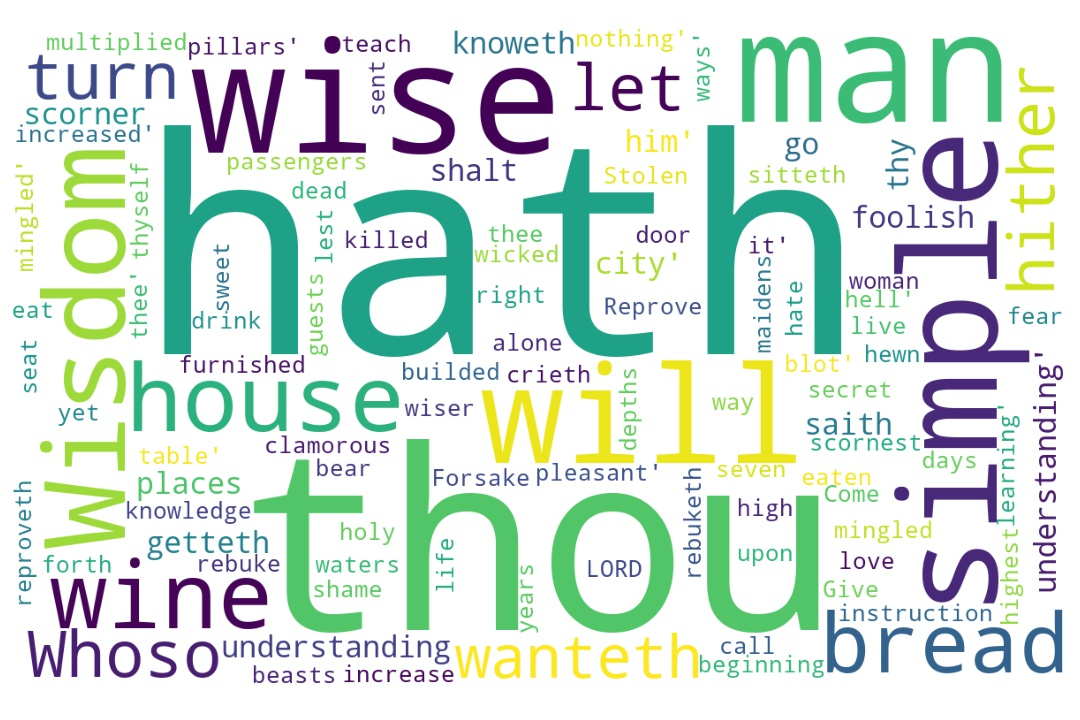
\includegraphics[width=\linewidth]{20OT-Proverbs/Proverb9-WordCloud.jpg}
  \caption{Proverb 9 Word Cloud}
  \label{fig:Proverb 9 Word Cloud}
\end{figure}


\marginpar{\scriptsize \centering \fcolorbox{bone}{lime}{\textbf{WISDOM: THE GOOD CHOICE}}\\ (Proverb 9:1-18) \begin{compactenum}[I.][8]
\item \textbf{Builds} a Life \index[scripture]{Proverbs!Pro 09:01}(Pro 9:1)
\item Has a \textbf{Banquet} \index[scripture]{Proverbs!Pro 09:02}(Pro 9:2)
\item Gives out \textbf{Bread} \index[scripture]{Proverbs!Pro 09:05}(Pro 9:5)
\item Has \textbf{Blessings} \index[scripture]{Proverbs!Pro 09:09}(Pro 9:9)
\item Was there from the \textbf{Beginning} \index[scripture]{Proverbs!Pro 09:10}(Pro 9:10)
\item Provides Lasting \textbf{Benefits} \index[scripture]{Proverbs!Pro 09:11}(Pro 9:11)
\item Is \textbf{Betrayed} \index[scripture]{Proverbs!Pro 09:13}(Pro 9:13)
\end{compactenum}}

\marginpar{\scriptsize \centering \fcolorbox{bone}{yellow}{\textbf{WISDOM AT WORK}}\\ (Proverb 9:1-18) \begin{compactenum}[I.][8]
    \item \textbf{Builds a House} \index[scripture]{Proverbs!Pro 09:01}(Pro 9:1)
    \item \textbf{Hews out Pillars} \index[scripture]{Proverbs!Pro 09:01}(Pro 9:1)
    \item \textbf{Kills her Beats} \index[scripture]{Proverbs!Pro 09:02}(Pro 9:2)
    \item \textbf{Mingles Her Wine} \index[scripture]{Proverbs!Pro 09:02}(Pro 9:2)
    \item \textbf{Furnishes her Table} \index[scripture]{Proverbs!Pro 09:02}(Pro 9:2)
    \item \textbf{Sends forthe her Maidens} \index[scripture]{Proverbs!Pro 09:03}(Pro 9:3)
    \item \textbf{Cries from the High Places} \index[scripture]{Proverbs!Pro 09:03}(Pro 9:3)
\end{compactenum}}

\marginpar{\scriptsize \centering \fcolorbox{bone}{black}{\textbf{\textcolor[cmyk]{0,0,0,0}{LOOKING FOR WISDOM}}}\\ (Proverb 9) 
\begin{compactenum}[I.][8]
    \item The \textbf{Rendering of Wisdom} \index[scripture]{Proverbs!Pro 09:01}(Pro 9:1) 
   \item The \textbf{Reaction to Wisdom} \index[scripture]{Proverbs!Pro 09:09}(Pro 9:9) 
    \item The \textbf{Reach for Wisdom} \index[scripture]{Proverbs!Pro 09:10}(Pro 9:10) 
    \item The \textbf{Road to Wisdom} \index[scripture]{Proverbs!Pro 09:11}(Pro 9:11) 
    \item The \textbf{Rejection of Wisdom} \index[scripture]{Proverbs!Pro 09:13}(Pro 9:13) 
    \item Man's \textbf{Regard \& Reverence for Foolishness} \index[scripture]{Proverbs!Pro 09:14}(Pro 9:14) 
    \item A \textbf{Reunion of Fools} \index[scripture]{Proverbs!Pro 09:15}(Pro 9:15) 
\end{compactenum}}

\footnote{\textcolor[cmyk]{0.99998,1,0,0}{\hyperlink{TOC}{Return to end of Table of Contents.}}}\footnote{\href{https://audiobible.com/bible/proverbs_9.html}{\textcolor[cmyk]{0.99998,1,0,0}{Proverbs Audio}}}\textcolor[cmyk]{0.99998,1,0,0}{Wisdom hath \fcolorbox{bone}{lime}{builded her house}, she hath hewn out her seven pillars:}\footnote{\textbf{1 Kings 8:27} - But will God indeed dwell on the earth? behold, the heaven and heaven of heavens cannot contain thee; how much less this house that I have builded?} 
[2] \textcolor[cmyk]{0.99998,1,0,0}{She hath killed her beasts; she hath mingled her wine; she hath also \fcolorbox{bone}{lime}{furnished} her table.}
[3] \textcolor[cmyk]{0.99998,1,0,0}{She hath sent forth her maidens: she crieth upon the highest places of the city,}
[4] \textcolor[cmyk]{0.99998,1,0,0}{Whoso \emph{is} simple, let him turn in hither: \emph{as} \emph{for} him that wanteth \fcolorbox{bone}{MYGOLD}{understanding}, she saith to him,}
[5] \textcolor[cmyk]{0.99998,1,0,0}{Come, \fcolorbox{bone}{lime}{eat of my} \fcolorbox{bone}{lime}{bread}, and drink of the wine \emph{which} I have mingled.}
[6] \textcolor[cmyk]{0.99998,1,0,0}{Forsake the foolish, and live; and go in the way of \fcolorbox{bone}{MYGOLD}{understanding}.}
[7] \textcolor[cmyk]{0.99998,1,0,0}{He that reproveth a scorner getteth to himself shame: and he that rebuketh a wicked \emph{man} \emph{getteth} himself a blot.}
[8] \textcolor[cmyk]{0.99998,1,0,0}{Reprove not a scorner, lest he hate thee: rebuke a wise man, and he will love thee.}
[9] \textcolor[cmyk]{0.99998,1,0,0}{Give \emph{instruction} to a wise \emph{man}, and he will \fcolorbox{bone}{lime}{be yet wiser}: teach a just \emph{man}, and he will increase in learning.}
[10] \textcolor[cmyk]{0.99998,1,0,0}{The fear of the LORD \emph{is} the \fcolorbox{bone}{lime}{beginning of wisdom}: and the knowledge of the holy \emph{is} \fcolorbox{bone}{MYGOLD}{understanding}.}
[11] \textcolor[cmyk]{0.99998,1,0,0}{For by me thy days shall be multiplied, and the years of thy life shall be \fcolorbox{bone}{lime}{increased}.}
[12] \textcolor[cmyk]{0.99998,1,0,0}{If thou be wise, thou shalt be wise for thyself: but \emph{if} thou scornest, thou alone shalt bear \emph{it}.}
[13] \textcolor[cmyk]{0.99998,1,0,0}{A foolish woman \emph{is} clamorous: \emph{she} \emph{is} simple, and \fcolorbox{bone}{lime}{knoweth nothing}.}
[14] \textcolor[cmyk]{0.99998,1,0,0}{For she sitteth at the door of her house, on a seat in the high places of the city,}
[15] \textcolor[cmyk]{0.99998,1,0,0}{To call passengers who go right on their ways:}
[16] \textcolor[cmyk]{0.99998,1,0,0}{Whoso \emph{is} simple, let him turn in hither: and \emph{as} \emph{for} him that wanteth \fcolorbox{bone}{MYGOLD}{understanding}, she saith to him,}
[17] \textcolor[cmyk]{0.99998,1,0,0}{Stolen waters are sweet, and bread \emph{eaten} in secret is pleasant.}
[18] \textcolor[cmyk]{0.99998,1,0,0}{But he knoweth not that the dead \emph{are} there; \emph{and} \emph{that} her guests \emph{are} in the depths of hell.}



\index[NWIV]{12!Proverbs!Pro 9:1}\index[AWIP]{Wisdom!Proverbs!Pro 9:1}\index[AWIP]{hath!Proverbs!Pro 9:1}\index[AWIP]{hath!Proverbs!Pro 9:1 (2)}\index[AWIP]{builded!Proverbs!Pro 9:1}\index[AWIP]{her!Proverbs!Pro 9:1}\index[AWIP]{her!Proverbs!Pro 9:1 (2)}\index[AWIP]{house!Proverbs!Pro 9:1}\index[AWIP]{she!Proverbs!Pro 9:1}\index[AWIP]{hewn!Proverbs!Pro 9:1}\index[AWIP]{out!Proverbs!Pro 9:1}\index[AWIP]{seven!Proverbs!Pro 9:1}\index[AWIP]{pillars!Proverbs!Pro 9:1}

\index[NWIV]{16!Proverbs!Pro 9:2}\index[AWIP]{She!Proverbs!Pro 9:2}\index[AWIP]{hath!Proverbs!Pro 9:2}\index[AWIP]{hath!Proverbs!Pro 9:2 (2)}\index[AWIP]{hath!Proverbs!Pro 9:2 (3)}\index[AWIP]{killed!Proverbs!Pro 9:2}\index[AWIP]{her!Proverbs!Pro 9:2}\index[AWIP]{her!Proverbs!Pro 9:2 (2)}\index[AWIP]{her!Proverbs!Pro 9:2 (3)}\index[AWIP]{beasts!Proverbs!Pro 9:2}\index[AWIP]{she!Proverbs!Pro 9:2}\index[AWIP]{she!Proverbs!Pro 9:2 (2)}\index[AWIP]{mingled!Proverbs!Pro 9:2}\index[AWIP]{wine!Proverbs!Pro 9:2}\index[AWIP]{also!Proverbs!Pro 9:2}\index[AWIP]{furnished!Proverbs!Pro 9:2}\index[AWIP]{table!Proverbs!Pro 9:2}

\index[NWIV]{15!Proverbs!Pro 9:3}\index[AWIP]{She!Proverbs!Pro 9:3}\index[AWIP]{hath!Proverbs!Pro 9:3}\index[AWIP]{sent!Proverbs!Pro 9:3}\index[AWIP]{forth!Proverbs!Pro 9:3}\index[AWIP]{her!Proverbs!Pro 9:3}\index[AWIP]{maidens!Proverbs!Pro 9:3}\index[AWIP]{she!Proverbs!Pro 9:3}\index[AWIP]{crieth!Proverbs!Pro 9:3}\index[AWIP]{upon!Proverbs!Pro 9:3}\index[AWIP]{the!Proverbs!Pro 9:3}\index[AWIP]{the!Proverbs!Pro 9:3 (2)}\index[AWIP]{highest!Proverbs!Pro 9:3}\index[AWIP]{places!Proverbs!Pro 9:3}\index[AWIP]{of!Proverbs!Pro 9:3}\index[AWIP]{city!Proverbs!Pro 9:3}

\index[NWIV]{18!Proverbs!Pro 9:4}\index[AWIP]{Whoso!Proverbs!Pro 9:4}\index[AWIP]{\emph{is}!Proverbs!Pro 9:4}\index[AWIP]{simple!Proverbs!Pro 9:4}\index[AWIP]{let!Proverbs!Pro 9:4}\index[AWIP]{him!Proverbs!Pro 9:4}\index[AWIP]{him!Proverbs!Pro 9:4 (2)}\index[AWIP]{him!Proverbs!Pro 9:4 (3)}\index[AWIP]{turn!Proverbs!Pro 9:4}\index[AWIP]{in!Proverbs!Pro 9:4}\index[AWIP]{hither!Proverbs!Pro 9:4}\index[AWIP]{\emph{as}!Proverbs!Pro 9:4}\index[AWIP]{\emph{for}!Proverbs!Pro 9:4}\index[AWIP]{that!Proverbs!Pro 9:4}\index[AWIP]{wanteth!Proverbs!Pro 9:4}\index[AWIP]{understanding!Proverbs!Pro 9:4}\index[AWIP]{she!Proverbs!Pro 9:4}\index[AWIP]{saith!Proverbs!Pro 9:4}\index[AWIP]{to!Proverbs!Pro 9:4}\index[AWIP]{\emph{is}!Proverbs!Pro 9:4}\index[AWIP]{\emph{as}!Proverbs!Pro 9:4}\index[AWIP]{\emph{for}!Proverbs!Pro 9:4}

\index[NWIV]{14!Proverbs!Pro 9:5}\index[AWIP]{Come!Proverbs!Pro 9:5}\index[AWIP]{eat!Proverbs!Pro 9:5}\index[AWIP]{of!Proverbs!Pro 9:5}\index[AWIP]{of!Proverbs!Pro 9:5 (2)}\index[AWIP]{my!Proverbs!Pro 9:5}\index[AWIP]{bread!Proverbs!Pro 9:5}\index[AWIP]{and!Proverbs!Pro 9:5}\index[AWIP]{drink!Proverbs!Pro 9:5}\index[AWIP]{the!Proverbs!Pro 9:5}\index[AWIP]{wine!Proverbs!Pro 9:5}\index[AWIP]{\emph{which}!Proverbs!Pro 9:5}\index[AWIP]{I!Proverbs!Pro 9:5}\index[AWIP]{have!Proverbs!Pro 9:5}\index[AWIP]{mingled!Proverbs!Pro 9:5}\index[AWIP]{\emph{which}!Proverbs!Pro 9:5}

\index[NWIV]{12!Proverbs!Pro 9:6}\index[AWIP]{Forsake!Proverbs!Pro 9:6}\index[AWIP]{the!Proverbs!Pro 9:6}\index[AWIP]{the!Proverbs!Pro 9:6 (2)}\index[AWIP]{foolish!Proverbs!Pro 9:6}\index[AWIP]{and!Proverbs!Pro 9:6}\index[AWIP]{and!Proverbs!Pro 9:6 (2)}\index[AWIP]{live!Proverbs!Pro 9:6}\index[AWIP]{go!Proverbs!Pro 9:6}\index[AWIP]{in!Proverbs!Pro 9:6}\index[AWIP]{way!Proverbs!Pro 9:6}\index[AWIP]{of!Proverbs!Pro 9:6}\index[AWIP]{understanding!Proverbs!Pro 9:6}

\index[NWIV]{20!Proverbs!Pro 9:7}\index[AWIP]{He!Proverbs!Pro 9:7}\index[AWIP]{that!Proverbs!Pro 9:7}\index[AWIP]{that!Proverbs!Pro 9:7 (2)}\index[AWIP]{reproveth!Proverbs!Pro 9:7}\index[AWIP]{a!Proverbs!Pro 9:7}\index[AWIP]{a!Proverbs!Pro 9:7 (2)}\index[AWIP]{a!Proverbs!Pro 9:7 (3)}\index[AWIP]{scorner!Proverbs!Pro 9:7}\index[AWIP]{getteth!Proverbs!Pro 9:7}\index[AWIP]{to!Proverbs!Pro 9:7}\index[AWIP]{himself!Proverbs!Pro 9:7}\index[AWIP]{himself!Proverbs!Pro 9:7 (2)}\index[AWIP]{shame!Proverbs!Pro 9:7}\index[AWIP]{and!Proverbs!Pro 9:7}\index[AWIP]{he!Proverbs!Pro 9:7}\index[AWIP]{rebuketh!Proverbs!Pro 9:7}\index[AWIP]{wicked!Proverbs!Pro 9:7}\index[AWIP]{\emph{man}!Proverbs!Pro 9:7}\index[AWIP]{\emph{getteth}!Proverbs!Pro 9:7}\index[AWIP]{blot!Proverbs!Pro 9:7}\index[AWIP]{\emph{man}!Proverbs!Pro 9:7}\index[AWIP]{\emph{getteth}!Proverbs!Pro 9:7}

\index[NWIV]{17!Proverbs!Pro 9:8}\index[AWIP]{Reprove!Proverbs!Pro 9:8}\index[AWIP]{not!Proverbs!Pro 9:8}\index[AWIP]{a!Proverbs!Pro 9:8}\index[AWIP]{a!Proverbs!Pro 9:8 (2)}\index[AWIP]{scorner!Proverbs!Pro 9:8}\index[AWIP]{lest!Proverbs!Pro 9:8}\index[AWIP]{he!Proverbs!Pro 9:8}\index[AWIP]{he!Proverbs!Pro 9:8 (2)}\index[AWIP]{hate!Proverbs!Pro 9:8}\index[AWIP]{thee!Proverbs!Pro 9:8}\index[AWIP]{thee!Proverbs!Pro 9:8 (2)}\index[AWIP]{rebuke!Proverbs!Pro 9:8}\index[AWIP]{wise!Proverbs!Pro 9:8}\index[AWIP]{man!Proverbs!Pro 9:8}\index[AWIP]{and!Proverbs!Pro 9:8}\index[AWIP]{will!Proverbs!Pro 9:8}\index[AWIP]{love!Proverbs!Pro 9:8}

\index[NWIV]{22!Proverbs!Pro 9:9}\index[AWIP]{Give!Proverbs!Pro 9:9}\index[AWIP]{\emph{instruction}!Proverbs!Pro 9:9}\index[AWIP]{to!Proverbs!Pro 9:9}\index[AWIP]{a!Proverbs!Pro 9:9}\index[AWIP]{a!Proverbs!Pro 9:9 (2)}\index[AWIP]{wise!Proverbs!Pro 9:9}\index[AWIP]{\emph{man}!Proverbs!Pro 9:9}\index[AWIP]{\emph{man}!Proverbs!Pro 9:9 (2)}\index[AWIP]{and!Proverbs!Pro 9:9}\index[AWIP]{and!Proverbs!Pro 9:9 (2)}\index[AWIP]{he!Proverbs!Pro 9:9}\index[AWIP]{he!Proverbs!Pro 9:9 (2)}\index[AWIP]{will!Proverbs!Pro 9:9}\index[AWIP]{will!Proverbs!Pro 9:9 (2)}\index[AWIP]{be!Proverbs!Pro 9:9}\index[AWIP]{yet!Proverbs!Pro 9:9}\index[AWIP]{wiser!Proverbs!Pro 9:9}\index[AWIP]{teach!Proverbs!Pro 9:9}\index[AWIP]{just!Proverbs!Pro 9:9}\index[AWIP]{increase!Proverbs!Pro 9:9}\index[AWIP]{in!Proverbs!Pro 9:9}\index[AWIP]{learning!Proverbs!Pro 9:9}\index[AWIP]{\emph{instruction}!Proverbs!Pro 9:9}\index[AWIP]{\emph{man}!Proverbs!Pro 9:9}\index[AWIP]{\emph{man}!Proverbs!Pro 9:9 (2)}

\index[NWIV]{18!Proverbs!Pro 9:10}\index[AWIP]{The!Proverbs!Pro 9:10}\index[AWIP]{fear!Proverbs!Pro 9:10}\index[AWIP]{of!Proverbs!Pro 9:10}\index[AWIP]{of!Proverbs!Pro 9:10 (2)}\index[AWIP]{of!Proverbs!Pro 9:10 (3)}\index[AWIP]{the!Proverbs!Pro 9:10}\index[AWIP]{the!Proverbs!Pro 9:10 (2)}\index[AWIP]{the!Proverbs!Pro 9:10 (3)}\index[AWIP]{the!Proverbs!Pro 9:10 (4)}\index[AWIP]{LORD!Proverbs!Pro 9:10}\index[AWIP]{\emph{is}!Proverbs!Pro 9:10}\index[AWIP]{\emph{is}!Proverbs!Pro 9:10 (2)}\index[AWIP]{beginning!Proverbs!Pro 9:10}\index[AWIP]{wisdom!Proverbs!Pro 9:10}\index[AWIP]{and!Proverbs!Pro 9:10}\index[AWIP]{knowledge!Proverbs!Pro 9:10}\index[AWIP]{holy!Proverbs!Pro 9:10}\index[AWIP]{understanding!Proverbs!Pro 9:10}\index[AWIP]{\emph{is}!Proverbs!Pro 9:10}\index[AWIP]{\emph{is}!Proverbs!Pro 9:10 (2)}

\index[NWIV]{17!Proverbs!Pro 9:11}\index[AWIP]{For!Proverbs!Pro 9:11}\index[AWIP]{by!Proverbs!Pro 9:11}\index[AWIP]{me!Proverbs!Pro 9:11}\index[AWIP]{thy!Proverbs!Pro 9:11}\index[AWIP]{thy!Proverbs!Pro 9:11 (2)}\index[AWIP]{days!Proverbs!Pro 9:11}\index[AWIP]{shall!Proverbs!Pro 9:11}\index[AWIP]{shall!Proverbs!Pro 9:11 (2)}\index[AWIP]{be!Proverbs!Pro 9:11}\index[AWIP]{be!Proverbs!Pro 9:11 (2)}\index[AWIP]{multiplied!Proverbs!Pro 9:11}\index[AWIP]{and!Proverbs!Pro 9:11}\index[AWIP]{the!Proverbs!Pro 9:11}\index[AWIP]{years!Proverbs!Pro 9:11}\index[AWIP]{of!Proverbs!Pro 9:11}\index[AWIP]{life!Proverbs!Pro 9:11}\index[AWIP]{increased!Proverbs!Pro 9:11}

\index[NWIV]{19!Proverbs!Pro 9:12}\index[AWIP]{If!Proverbs!Pro 9:12}\index[AWIP]{thou!Proverbs!Pro 9:12}\index[AWIP]{thou!Proverbs!Pro 9:12 (2)}\index[AWIP]{thou!Proverbs!Pro 9:12 (3)}\index[AWIP]{thou!Proverbs!Pro 9:12 (4)}\index[AWIP]{be!Proverbs!Pro 9:12}\index[AWIP]{be!Proverbs!Pro 9:12 (2)}\index[AWIP]{wise!Proverbs!Pro 9:12}\index[AWIP]{wise!Proverbs!Pro 9:12 (2)}\index[AWIP]{shalt!Proverbs!Pro 9:12}\index[AWIP]{shalt!Proverbs!Pro 9:12 (2)}\index[AWIP]{for!Proverbs!Pro 9:12}\index[AWIP]{thyself!Proverbs!Pro 9:12}\index[AWIP]{but!Proverbs!Pro 9:12}\index[AWIP]{\emph{if}!Proverbs!Pro 9:12}\index[AWIP]{scornest!Proverbs!Pro 9:12}\index[AWIP]{alone!Proverbs!Pro 9:12}\index[AWIP]{bear!Proverbs!Pro 9:12}\index[AWIP]{\emph{it}!Proverbs!Pro 9:12}\index[AWIP]{\emph{if}!Proverbs!Pro 9:12}\index[AWIP]{\emph{it}!Proverbs!Pro 9:12}

\index[NWIV]{11!Proverbs!Pro 9:13}\index[AWIP]{A!Proverbs!Pro 9:13}\index[AWIP]{foolish!Proverbs!Pro 9:13}\index[AWIP]{woman!Proverbs!Pro 9:13}\index[AWIP]{\emph{is}!Proverbs!Pro 9:13}\index[AWIP]{\emph{is}!Proverbs!Pro 9:13 (2)}\index[AWIP]{clamorous!Proverbs!Pro 9:13}\index[AWIP]{\emph{she}!Proverbs!Pro 9:13}\index[AWIP]{simple!Proverbs!Pro 9:13}\index[AWIP]{and!Proverbs!Pro 9:13}\index[AWIP]{knoweth!Proverbs!Pro 9:13}\index[AWIP]{nothing!Proverbs!Pro 9:13}\index[AWIP]{\emph{is}!Proverbs!Pro 9:13}\index[AWIP]{\emph{is}!Proverbs!Pro 9:13 (2)}\index[AWIP]{\emph{she}!Proverbs!Pro 9:13}

\index[NWIV]{19!Proverbs!Pro 9:14}\index[AWIP]{For!Proverbs!Pro 9:14}\index[AWIP]{she!Proverbs!Pro 9:14}\index[AWIP]{sitteth!Proverbs!Pro 9:14}\index[AWIP]{at!Proverbs!Pro 9:14}\index[AWIP]{the!Proverbs!Pro 9:14}\index[AWIP]{the!Proverbs!Pro 9:14 (2)}\index[AWIP]{the!Proverbs!Pro 9:14 (3)}\index[AWIP]{door!Proverbs!Pro 9:14}\index[AWIP]{of!Proverbs!Pro 9:14}\index[AWIP]{of!Proverbs!Pro 9:14 (2)}\index[AWIP]{her!Proverbs!Pro 9:14}\index[AWIP]{house!Proverbs!Pro 9:14}\index[AWIP]{on!Proverbs!Pro 9:14}\index[AWIP]{a!Proverbs!Pro 9:14}\index[AWIP]{seat!Proverbs!Pro 9:14}\index[AWIP]{in!Proverbs!Pro 9:14}\index[AWIP]{high!Proverbs!Pro 9:14}\index[AWIP]{places!Proverbs!Pro 9:14}\index[AWIP]{city!Proverbs!Pro 9:14}

\index[NWIV]{9!Proverbs!Pro 9:15}\index[AWIP]{To!Proverbs!Pro 9:15}\index[AWIP]{call!Proverbs!Pro 9:15}\index[AWIP]{passengers!Proverbs!Pro 9:15}\index[AWIP]{who!Proverbs!Pro 9:15}\index[AWIP]{go!Proverbs!Pro 9:15}\index[AWIP]{right!Proverbs!Pro 9:15}\index[AWIP]{on!Proverbs!Pro 9:15}\index[AWIP]{their!Proverbs!Pro 9:15}\index[AWIP]{ways!Proverbs!Pro 9:15}

\index[NWIV]{19!Proverbs!Pro 9:16}\index[AWIP]{Whoso!Proverbs!Pro 9:16}\index[AWIP]{\emph{is}!Proverbs!Pro 9:16}\index[AWIP]{simple!Proverbs!Pro 9:16}\index[AWIP]{let!Proverbs!Pro 9:16}\index[AWIP]{him!Proverbs!Pro 9:16}\index[AWIP]{him!Proverbs!Pro 9:16 (2)}\index[AWIP]{him!Proverbs!Pro 9:16 (3)}\index[AWIP]{turn!Proverbs!Pro 9:16}\index[AWIP]{in!Proverbs!Pro 9:16}\index[AWIP]{hither!Proverbs!Pro 9:16}\index[AWIP]{and!Proverbs!Pro 9:16}\index[AWIP]{\emph{as}!Proverbs!Pro 9:16}\index[AWIP]{\emph{for}!Proverbs!Pro 9:16}\index[AWIP]{that!Proverbs!Pro 9:16}\index[AWIP]{wanteth!Proverbs!Pro 9:16}\index[AWIP]{understanding!Proverbs!Pro 9:16}\index[AWIP]{she!Proverbs!Pro 9:16}\index[AWIP]{saith!Proverbs!Pro 9:16}\index[AWIP]{to!Proverbs!Pro 9:16}\index[AWIP]{\emph{is}!Proverbs!Pro 9:16}\index[AWIP]{\emph{as}!Proverbs!Pro 9:16}\index[AWIP]{\emph{for}!Proverbs!Pro 9:16}

\index[NWIV]{11!Proverbs!Pro 9:17}\index[AWIP]{Stolen!Proverbs!Pro 9:17}\index[AWIP]{waters!Proverbs!Pro 9:17}\index[AWIP]{are!Proverbs!Pro 9:17}\index[AWIP]{sweet!Proverbs!Pro 9:17}\index[AWIP]{and!Proverbs!Pro 9:17}\index[AWIP]{bread!Proverbs!Pro 9:17}\index[AWIP]{\emph{eaten}!Proverbs!Pro 9:17}\index[AWIP]{in!Proverbs!Pro 9:17}\index[AWIP]{secret!Proverbs!Pro 9:17}\index[AWIP]{is!Proverbs!Pro 9:17}\index[AWIP]{pleasant!Proverbs!Pro 9:17}\index[AWIP]{\emph{eaten}!Proverbs!Pro 9:17}

\index[NWIV]{19!Proverbs!Pro 9:18}\index[AWIP]{But!Proverbs!Pro 9:18}\index[AWIP]{he!Proverbs!Pro 9:18}\index[AWIP]{knoweth!Proverbs!Pro 9:18}\index[AWIP]{not!Proverbs!Pro 9:18}\index[AWIP]{that!Proverbs!Pro 9:18}\index[AWIP]{the!Proverbs!Pro 9:18}\index[AWIP]{the!Proverbs!Pro 9:18 (2)}\index[AWIP]{dead!Proverbs!Pro 9:18}\index[AWIP]{\emph{are}!Proverbs!Pro 9:18}\index[AWIP]{\emph{are}!Proverbs!Pro 9:18 (2)}\index[AWIP]{there!Proverbs!Pro 9:18}\index[AWIP]{\emph{and}!Proverbs!Pro 9:18}\index[AWIP]{\emph{that}!Proverbs!Pro 9:18}\index[AWIP]{her!Proverbs!Pro 9:18}\index[AWIP]{guests!Proverbs!Pro 9:18}\index[AWIP]{in!Proverbs!Pro 9:18}\index[AWIP]{depths!Proverbs!Pro 9:18}\index[AWIP]{of!Proverbs!Pro 9:18}\index[AWIP]{hell!Proverbs!Pro 9:18}\index[AWIP]{\emph{are}!Proverbs!Pro 9:18}\index[AWIP]{\emph{are}!Proverbs!Pro 9:18 (2)}\index[AWIP]{\emph{and}!Proverbs!Pro 9:18}\index[AWIP]{\emph{that}!Proverbs!Pro 9:18}


\section{Proverbs 9 Outlines}

\subsection{My Outlines}

\subsubsection{Wisdom: The Good Choice}
\index[speaker]{Keith Anthony!Proverb 09 (Wisdom: The Good Choice)}
\index[series]{Proverbs (Keith Anthony)!Pro 09 (Wisdom: The Good Choice)}
\index[date]{2016/05/09!Proverb 09  (Wisdom: The Good Choice)}
%\textbf{Lineage}: adpated from S. Conway\\
\textbf{Introduction}: In Proverbs 9, wisdom and folly both invite men to take part in them. Folly invites those walking a straight (right) path (verse 15) to turn unto a way that ends in the depths of hell (verse 18).  But the path of wisdom:
\begin{compactenum}[I.]
\item \textbf{Builds} a Life \index[scripture]{Proverbs!Pro 09:01}(Pro 9:1)
\item Has a \textbf{Banquet} \index[scripture]{Proverbs!Pro 09:02}(Pro 9:2)
\item Gives out \textbf{Bread} \index[scripture]{Proverbs!Pro 09:05}(Pro 9:5)
\item Has \textbf{Blessings} \index[scripture]{Proverbs!Pro 09:09}(Pro 9:9)
\item Was there from the \textbf{Beginning} \index[scripture]{Proverbs!Pro 09:10}(Pro 9:10)
\item Provides Lasting \textbf{Benefits} \index[scripture]{Proverbs!Pro 09:11}(Pro 9:11)
\item Is \textbf{Betrayed} \index[scripture]{Proverbs!Pro 09:13}(Pro 9:13)
\end{compactenum}

\subsubsection{Wisdom at Work}
\index[speaker]{Keith Anthony!Proverb 09 (Wisdom at Work)}
\index[series]{Proverbs (Keith Anthony)!Pro 09 (Wisdom at Work)}
\index[date]{2016/05/09!Proverb 09 (Wisdom is There) (Wisdom at Work)}
\textbf{Introduction}: Proverbs 9:1-3 lists the activities of wisdom:\footnote{9 June 2016, Keith Anthony}
\begin{compactenum}[I.][7]
    \item \textbf{Builds a House} \index[scripture]{Proverbs!Pro 09:01}(Pro 9:1)
    \item \textbf{Hews out Pillars} \index[scripture]{Proverbs!Pro 09:01}(Pro 9:1)
    \item \textbf{Kills her Beats} \index[scripture]{Proverbs!Pro 09:02}(Pro 9:2)
    \item \textbf{Mingles Her Wine} \index[scripture]{Proverbs!Pro 09:02}(Pro 9:2)
    \item \textbf{Furnishes her Table} \index[scripture]{Proverbs!Pro 09:02}(Pro 9:2)
    \item \textbf{Sends forthe her Maidens} \index[scripture]{Proverbs!Pro 09:03}(Pro 9:3)
    \item \textbf{Cries from the High Places} \index[scripture]{Proverbs!Pro 09:03}(Pro 9:3)
\end{compactenum}

\subsubsection{Looking for Wisdom}
%\textbf{Introduction:} Wisdom not only delivers one from evil, but promises certain rewards:
%\footnote{03 November 2014, Keith Anthony}
\index[speaker]{Keith Anthony!Proverb 09 (Looking for Wisdom)}
\index[series]{Proverbs (Keith Anthony)!Pro 09 (Looking for Wisdom)}
\index[date]{2017/01/09!Proverb 09 (Looking for Wisdom) (Keith Anthony)}
\begin{compactenum}[I.][7]
    \item The \textbf{Rendering of Wisdom} \index[scripture]{Proverbs!Pro 09:01}(Pro 9:1) 
    \item The \textbf{Reaction to Wisdom} \index[scripture]{Proverbs!Pro 09:09}(Pro 9:9) 
    \item The \textbf{Reach for Wisdom} \index[scripture]{Proverbs!Pro 09:10}(Pro 9:10) 
    \item The \textbf{Road to Wisdom} \index[scripture]{Proverbs!Pro 09:11}(Pro 9:11) 
    \item The \textbf{Rejection of Wisdom} \index[scripture]{Proverbs!Pro 09:13}(Pro 9:13) 
    \item Man's \textbf{Regard \& Reverence for Foolishness} \index[scripture]{Proverbs!Pro 09:14}(Pro 9:14) 
    \item A \textbf{Reunion of Fools} \index[scripture]{Proverbs!Pro 09:15}(Pro 9:15) 
\end{compactenum}

\subsection{Outlines from Others}


\section{Proverb 9 Comments}

\subsection{Numeric Nuggets}
\textbf{13:} The 13-letter word ``understanding'' is used in Proverb 9. Verses 5 and 12 have 13 unique words. The word ``and'' is used 13 times, one instance in italics.

\subsection{Proverb 9:1}
What about these seven pillars?
\begin{compactenum}
    \item One respected preacher identifies these seven pillars as the seven descriptions of the Word of God found in Psalm 119.
    \item William Grady maps the seven pillars of wisdom to 2 Peter 2:4-7: (1) faith, (2) virtue, (3) knowledge, (4) temperance, (5) godliness, (6) brotherly kindness, and (7) charity. These pillars would map to seven physical pillars around the temple: 3 of the south side, temperance on the west, and the remaining three heading back toward the Temple opening on the north \cite{grady2010given}. This is the interpretation which I think fits best.
    \item Henry Morris, of the Institute for Creation Research (ICR), has the seven pillars listed in James 3:17:  (1) genuine purity, (2) peaceableness, (3) gentleness, (4) reasonableness, (5) helpfulness, (6) humility, and (7) sincerity. But these words are not found in the AV1611.  Instead are adjectives describing wisdom.
    \item Some equate these 7 pillars withe seven divisions of Proverbs: identified in (1) Proverbs 1:1 "The proverbs of Solomon", (2) Proverbs 10:1 "The proverbs of Solomon", (3) Proverbs 22:17 "hear the words of the wise", (4) Proverbs 24:23 "These things also belong to the wise", (5) Proverbs 25:1 "These are also the proverbs of Solomon", (6) Proverbs 30:1 "The words of A'gur... even the prophecy...", and (7) Proverbs 31:1.
    \item But, noting the septatic (7) structure found throughout scripture, some equate the pillars to the seven main sections of the Bible: (1) Torah/Law,(2) OT History, (3) Wisdom Books, (4) Major Prophets, (5) Minor Prophets, (6) NT History, and (7) NT Epistles.
    \item William Brown, in The Seven Pillars of Creation: The Bible, Science, and the Ecology of Wonder, cites Rabbinical scholars who equated these pillars with the seven days of creation. \cite{brown2010SevenPillars}
\end{compactenum}

\subsection{Proverb 9:7, 8}
The verses say to not waste your time with a scorner.

\subsection{Proverb 9:13}
This is the only use of the word ``clamorous'' in the KJV. Webster's has three definitions of the word. First. Clamorous is one who ``engages in or is marked by loud and insistent cries especially of protest."  Clamorous is ``full of or characterized by the presence of noise.'' And clamorous is ``marked by a high volume of sound.''  A list of synonyms includes: blatant, caterwauling, clamant, obstreperous, squawking, vociferant, vociferating, vociferous, yawping (or yauping), yowling, clangorous, clattering, clattery, noisy, rackety, resounding, uproarious, blaring, blasting, booming, deafening, earsplitting, loud, piercing, plangent, resounding, ringing, roaring, slam-bang, sonorous, stentorian, thundering, and thunderous. 

\subsection{Proverb 9:15}
The word ``wanteth'' here. is understood as ``lacks.'' The foolish and clamorous woman is not speaking to the one with understanding, but the one who does not have any.


\subsection{Proverb 9 Repeated Phrases}


%%%%%%%%%%
%%%%%%%%%%
\normalsize
 
\begin{center}
\begin{longtable}{|p{3.0in}|p{0.5in}|}
\caption[Proverb 9 Repeated Phrases]{Proverb 9 Repeated Phrases}\label{table:Repeated Phrases Proverb 9} \\
\hline \multicolumn{1}{|c|}{\textbf{Phrase}} & \multicolumn{1}{c|}{\textbf{Frequency}} \\ \hline 
\endfirsthead
 
\multicolumn{2}{c}
{{\bfseries \tablename\ \thetable{} -- continued from previous page}} \\  
\hline \multicolumn{1}{|c|}{\textbf{Phrase}} & \multicolumn{1}{c|}{\textbf{Frequency}} \\ \hline 
\endhead
 
\hline \multicolumn{2}{c}{{ }} \\ \hline
\endfoot 
of the & 5\\ \hline 
and he & 4\\ \hline 
she hath & 3\\ \hline 
\emph{is} simple & 3\\ \hline 
in the & 3\\ \hline 
and he will & 3\\ \hline 
he will & 3\\ \hline 
\end{longtable}
\end{center}



%%%%%%%%%%
%%%%%%%%%%



%\newpage
\section{Proverb 9 Comments}

\subsection{Numeric Nuggets}
\textbf{13:} The 13-letter word ``understanding'' is used in Proverb 9. Verses 5 and 12 have 13 unique words. The word ``and'' is used 13 times, one instance in italics.

\subsection{Proverb 9:1}
What about these seven pillars?
\begin{compactenum}
    \item One respected preacher identifies these seven pillars as the seven descriptions of the Word of God found in Psalm 119.
    \item William Grady maps the seven pillars of wisdom to 2 Peter 2:4-7: (1) faith, (2) virtue, (3) knowledge, (4) temperance, (5) godliness, (6) brotherly kindness, and (7) charity. These pillars would map to seven physical pillars around the temple: 3 of the south side, temperance on the west, and the remaining three heading back toward the Temple opening on the north \cite{grady2010given}. This is the interpretation which I think fits best.
    \item Henry Morris, of the Institute for Creation Research (ICR), has the seven pillars listed in James 3:17:  (1) genuine purity, (2) peaceableness, (3) gentleness, (4) reasonableness, (5) helpfulness, (6) humility, and (7) sincerity. But these words are not found in the AV1611.  Instead are adjectives describing wisdom.
    \item Some equate these 7 pillars withe seven divisions of Proverbs: identified in (1) Proverbs 1:1 "The proverbs of Solomon", (2) Proverbs 10:1 "The proverbs of Solomon", (3) Proverbs 22:17 "hear the words of the wise", (4) Proverbs 24:23 "These things also belong to the wise", (5) Proverbs 25:1 "These are also the proverbs of Solomon", (6) Proverbs 30:1 "The words of A'gur... even the prophecy...", and (7) Proverbs 31:1.
    \item But, noting the septatic (7) structure found throughout scripture, some equate the pillars to the seven main sections of the Bible: (1) Torah/Law,(2) OT History, (3) Wisdom Books, (4) Major Prophets, (5) Minor Prophets, (6) NT History, and (7) NT Epistles.
    \item William Brown, in The Seven Pillars of Creation: The Bible, Science, and the Ecology of Wonder, cites Rabbinical scholars who equated these pillars with the seven days of creation. \cite{brown2010SevenPillars}
\end{compactenum}

\subsection{Proverb 9:7, 8}
The verses say to not waste your time with a scorner.

\subsection{Proverb 9:13}
This is the only use of the word ``clamorous'' in the KJV. Webster's has three definitions of the word. First. Clamorous is one who ``engages in or is marked by loud and insistent cries especially of protest."  Clamorous is ``full of or characterized by the presence of noise.'' And clamorous is ``marked by a high volume of sound.''  A list of synonyms includes: blatant, caterwauling, clamant, obstreperous, squawking, vociferant, vociferating, vociferous, yawping (or yauping), yowling, clangorous, clattering, clattery, noisy, rackety, resounding, uproarious, blaring, blasting, booming, deafening, earsplitting, loud, piercing, plangent, resounding, ringing, roaring, slam-bang, sonorous, stentorian, thundering, and thunderous. 

\subsection{Proverb 9:15}
The word ``wanteth'' here. is understood as ``lacks.'' The foolish and clamorous woman is not speaking to the one with understanding, but the one who does not have any.


%\input{20OT-Proverbs/Example-DEVOTIONAL-Psalm3-DEVOTIONAL-BryanChapel}



%%% For Indexes

%\index[DEVOTIONAL]{TGIF1!Os Hillman (Living for a Cause Greater Than Yourself) - Proverb 19:17!2021/12/21}

%\index[DEVOTIONAL]{TGIF1!Os Hillman (Living for a Cause Greater Than Yourself) - Proverb 19:17!2021/12/21}

















%%% colour: cardinal red - \textcolor[cmyk]{0,0.85,0.70,0.23}{text}


%%%% Example marginpar with a compactenum list --- green color text
%\marginpar{\scriptsize \textcolor[rgb]{0.00,0.545,0.269}{$\rightarrow$7 Abominations: 
%\begin{compactenum}
%	\item A proud look,
%	\item a lying tongue,
%	\item hands that shed innocent blood,
%	\item An heart that deviseth wicked imaginations,
%	\item feet that be swift in running to mischief,
%	\item A false witness that speaketh lies, and
%	\item he that soweth discord among brethren.
%\end{compactenum}}}



%\newpage

%\begin{mdframed}[style=MyFrame]
%\begin{center}
%\begin{longtable}{|p{.5in}|p{3.5in}|}

%\caption[Corruption Alert: Proverbs 18:1]{Corruption Alert: Proverbs 18:1} \label{table:CorruptionProv18:1} \\ 

%\hline  
%\multicolumn{1}{|c|}{\textbf{Version}} & 
%\multicolumn{1}{c|}{\textbf{Corruption}}  \\ \hline 
%\endfirsthead
 
%\multicolumn{2}{c}
%{{\bfseries \tablename\ \thetable{} -- continued from previous page}} \\  \hline  
%\multicolumn{1}{|c|}{\textbf{Version}} & 
%\multicolumn{1}{c|}{\textbf{Corruption}}  \\ \hline 
%\endhead
 
%\hline \multicolumn{2}{|r|}{{Continued on next page}} \\ \hline
%\endfoot 
%\textcolor[rgb]{0.00,0.00,1.00}{AV} & \textcolor[rgb]{0.00,0.00,1.00}{Through desire a man, having separated himself, seeketh \emph{and} intermeddleth with all wisdom.} \\ \hline
%
%ASV &  He that separateth himself seeketh his own desire, And  rageth against all sound wisdom. \\ \hline
%
%CEB &  Unfriendly people look out for themselves; they bicker with sensible people.\\ \hline
%
%ESV & Whoever isolates himself seeks his own desire;  he breaks out against all sound judgment. \\ \hline
%
%NASV &  He who separates himself seeks his own desire, He quarrels against all sound wisdom.\\ \hline
%
%MEV & He who separates himself seeks his own desire; he seeks and quarrels against all wisdom.\\ \hline
%
%NIV &  An unfriendly person pursues selfish ends and against all sound judgment starts quarrels. \\ \hline
%
%NKJV &  A man who isolates himself seeks his own desire; He rages against all wise judgment.\\ \hline
%
%RSV &  He who is estranged seeks pretexts  to break out against all sound judgment.\\ \hline

% \multicolumn{2}{p{4.3in}}{{Modern translations, such as the ASV and others, strike out the first part of the verse, concealing the intent of mankind in genewisdom clearly revealed in scripture. How wonderful is the obfuscated RSV text: ``He who is estranged seeks pretexts.'' What does THAT mean?}} \\ %\hline

%\hline

%\end{longtable}
%\end{center}

%\normalsize 
%\end{mdframed}

%\marginpar{\scriptsize \centering \fcolorbox{black}{lime}{\textbf{OUTIDE THE PLACE OF PROMISE}}\\ (Psalm 137:1--9) 
%\begin{compactenum}[I.][8]
%	\item \textbf{Plight \& Distress} \index[scripture]{Psalms!Psa 137:01} (Psalm 137:1)
%	\item The \textbf{Place Desired} \index[scripture]{Psalms!Psa 137:01} (Psalm 137:1)
%	\item \textbf{Pining \& Despiar} \index[scripture]{Psalms!Psa 137:02} (Psalm 137:2)
%	\item \textbf{Provoked \& Degraded}\index[scripture]{Psalms!Psa 137:03} (Psalm 137:3)
%	\item The \textbf{Predicament Described}\index[scripture]{Psalms!Psa 137:04} (Psalm 137:4)
%	\item A \textbf{Preference Decided}\index[scripture]{Psalms!Psa 137:06} (Psalm 137:6)
%	\item A \textbf{Prediction of Destruction}\index[scripture]{Psalms!Psa 137:08} (Psalm 137:8)
%\end{compactenum} }


%\subsection{Outlines from Others}

%\subsubsection{Words on Wisdom}
%\index[speaker]{John Battles!Proverbs 01 (Words on Wisdom)}
%\index[series]{Proverbs (John Battles)!Proverbs 01 (Words on Wisdom)}
%\index[date]{2016/01/20!Proverbs 01 (Words on Wisdom) (John Battles)}
%\textbf{Lineage}: adpated from S. Conway\\
%\textbf{Introduction}: Proverbs distinctly points out things that a fool does:
%\begin{compactenum}[I.][4]
%	\item \textbf{Welcome to Wisdom} \index[scripture]{Proverbs!Pro 01:01-09}(Proverbs 1:1-9)
%	\item \textbf{Warnings of Wisdom} \index[scripture]{Proverbs!Pro 01:10-19}(Proverbs 1:10-19).
%	\item \textbf{Woe of Wisdom} \index[scripture]{Proverbs!Pro 01:24-32}(Proverbs 1:24-32)
%	\item \textbf{Watchcare of Wisdom} \index[scripture]{Proverbs!Pro 01:33}(Proverbs 1:33).
%\end{compactenum}


%%%%% COLOR FOR MARGINPAR OUTLINES
%% 1  LIME - \marginpar{\scriptsize \centering \fcolorbox{black}{lime}{\textbf{TITLE}}\\ (Passage) 
%% 2. YELLOW - \marginpar{\scriptsize \centering \fcolorbox{black}{yellow}{\textbf{TITLE}}\\ (Passage) 
%% 3. Blue BGND, WHITE LETTERS - \marginpar{\scriptsize \centering \fcolorbox{black}{blue}{\textbf{\textcolor[cmyk]{0,0,0,0}{TITLE}}}\\ (Passage) 
%% 4. black BGND, WHITE LETTERS - \marginpar{\scriptsize \centering \fcolorbox{black}{black}{\textbf{\textcolor[cmyk]{0,0,0,0}{TITLE}}}\\ (Passage) 
%% 5. red BGND, WHITE LETTERS - \marginpar{\scriptsize \centering \fcolorbox{black}{red}{\textbf{\textcolor[cmyk]{0,0,0,0}{TITLE}}}\\ (Passage) 

%%%%%% INCLUSION OF GRAPHIC
%\newpage

%\begin{figure}
%\begin{center}
%\includegraphics[scale=0.5, angle=90]{07OT-Judges/References/b201107i1-large}
%\caption[Summary of the 13 Judges]{Summary of the 13 Judges}
%\label{fig:Summary of the 13 Judges}
%\end{center}
%\end{figure}


%%%%%%%%%%%
%%%%%%%%%%%

% SYTEMATIC THEOLOGY (10 + 2)
% Theology proper – The study of the character of God
% Angelology – The study of angels
% Biblical theology – The study of the Bible
% Christology – The study of Christ
% Ecclesiology – The study of the church
% Eschatology – The study of the end times[5]
% Hamartiology – The study of sin
% Pneumatology – The study of the Holy Spirit
% Soteriology – The study of salvation
% Theological anthropology – The study of the nature of humanity.
% ++
% Moral theology
% Bilical cosomolgy

%%%%%%%%%%%%%%
%%%%%%%%%%%%%%

% \footnote{\href{https://audiobible.com/bible/psalms_91.html}{\textcolor[cmyk]{0.99998,1,0,0}{Psalm 91 Audio}}}

% \marginpar{\scriptsize \centering \fcolorbox{black}{lime}{\textbf{JERUSALEM}}\\
% \fcolorbox{black}{lime}{\textbf{DON'T GO BACK TO EGYPT}} \\ (Isaiah 31:1--9) 

%%%%%%%%%%%%%%
%%% Extra Colors
%%% from https://latexcolor.blogspot.com/2019/10/list-of-latex-colors.html
%%%%%%%%%%%%%%
% \definecolor{champagne}{rgb}{0.97,0.91,0.81}
% \definecolor{bone}{rgb}{0.89,0.85,0.79}
%\titleJE
%

%%%%% EXAMPLE Index entry:
% \index[DOCTRINES]{Eschatology - Millennium!Psalms!Psa 069:036}

%%% for things found 13 times
%\fcolorbox{black}{bone}{TEXT}
\scriptsize

%%%%%%%%%%%%%%%%%%%%%%%%%%%%%
%Indices

\chapter{Indexes}
\printindex[DOCTRINES]
\printindex[scripture]
\printindex[speaker]
%\printindex[series]

\printindex[FACEBOOK]
\printindex[LOCATION]
\printindex[DEVOTIONAL]
\printindex[AWIP]

\printbibliography
\end{document}

